% PhD thesis template, Lund University
% Originally designed for the Faculty of Science: Astronomy and Theoretical Physics
% Reformatted to work with Overleaf

% Layout and typesetting: Daniel Michalik, with Berry Holl, Helene Jönsson, Jonas Palm, Samuel Stenberg, Vidar Aspelin
% Implementation and documentation: Daniel Michalik, Samuel Stenberg
%
% Credits to the past generations of students who contributed to the original
% versions of this latex template, in particular Berry Holl.
% 
% Compilation instructions: use "xelatex" (necessary for support of the fonts
% used by Lund University. The fonts need to be installed first, see README.txt
% for instructions).
%
% If you use (pdf)latex instead, the default latex fonts will be used. 
% That would be a pity, cause the Garamond/Frutiger suggestion by the
% University looks much nicer for your thesis!
%
% Special command to automatically make Mac's TeXshop use xelatex for this file:
% !TEX TS-program = XeLaTeX
%
\documentclass[11pt]{book} 

% Hide all the usepackage commands and definitions in a preamble file.
% Normally you should not need to edit it.

% Custom aliases
%\newcommand{\jpsi}{\rm J/$\psi$}
%\newcommand{\psip}{$\psi^\prime$}
%\newcommand{\jpsiDY}{\rm J/$\psi$\,/\,DY}
%\newcommand{\dd}{\mathrm{d}}
%\newcommand{\chic}{$\chi_{\rm c}$}
%\newcommand{\ezdc}{$E_{\rm ZDC}$}
%\newcommand{\red}{\textcolor{red}}
%\newcommand{\blue}{\textcolor{blue}}
\newcommand{\RT}{\ensuremath{R_{\rm T}}\xspace}
\newcommand{\RTmin}{\ensuremath{R_{\rm T,min}}\xspace}
\newcommand{\RTmax}{\ensuremath{R_{\rm T,max}}\xspace}
\newcommand{\NT}{\ensuremath{N_{\rm T}}\xspace}
\newcommand{\NTmin}{\ensuremath{N_{\rm T,min}}\xspace}
\newcommand{\NTmax}{\ensuremath{N_{\rm T,max}}\xspace}
\newcommand{\NTt}{\ensuremath{N_{\rm T}^{t}}\xspace}
\newcommand{\NTtt}{\ensuremath{N_{\rm T}^{t'}}\xspace}
\newcommand{\NTm}{\ensuremath{N_{\rm T}^{m}}\xspace}
\newcommand{\nevhat}{\ensuremath{\hat{n}_{\rm ev}}\xspace}
\newcommand{\nev}{\ensuremath{n_{\rm ev}}\xspace}

\newcommand{\ptlead}{\ensuremath{p_{\rm T}^{\rm leading}}\xspace}
\newcommand{\philead}{\ensuremath{\phi^{\rm leading}}\xspace}
\newcommand{\meannmpi}{\ensuremath{\langle n_{\rm MPI} \rangle}\xspace}
\newcommand{\nmpi}{\ensuremath{n_{\rm MPI}}\xspace}
\newcommand{\tracklet}{\ensuremath{N_{\text{tracklets}}^{\text{$|\eta| < 0.8$}}}\xspace}
\newcommand{\INELgtO}{\ensuremath{\text{INEL} > 0}\xspace}
\newcommand{\dndy}         {\ensuremath{\mathrm{d}N_\mathrm{ch}/\mathrm{d}y}\xspace}
\newcommand{\dndeta}       {\ensuremath{\mathrm{d}N_\mathrm{ch}/\mathrm{d}\eta}\xspace}
\newcommand{\myield}       {\ensuremath{\left<\mathrm{d}N/\mathrm{d}y\right>}\xspace}
\newcommand{\myieldpi}       {\ensuremath{\left<\mathrm{d}N_\mathrm{\pi}/\mathrm{d}y\right>}\xspace}

\newcommand{\avdndeta}     {\ensuremath{\langle\dndeta\rangle}\xspace}
\newcommand{\Npart}        {\ensuremath{N_\mathrm{part}}\xspace}
\newcommand{\Ncoll}        {\ensuremath{N_\mathrm{coll}}\xspace}

\newcommand{\Raa}{\ensuremath{\rm R_{AA}}\xspace}
\newcommand{\Rpa}{\ensuremath{\rm R_{pA}}\xspace}
\newcommand{\Rppb}{\ensuremath{R_{\rm pPb}}\xspace}

\newcommand{\cme}{\ensuremath{\sqrt{s}}\xspace}
\newcommand{\gev}{\ensuremath{{\rm GeV}/c}\xspace}
\newcommand{\auau}{\ensuremath{\rm Au\!-\!Au}\xspace}
%\newcommand{\ptopi}{\ensuremath{({\rm p+ \bar{p}}) / (\pi^{+}+\pi^{-})}\xspace}
\newcommand{\pikp}{\ensuremath{\pi/{\rm K}/{\rm p}}\xspace}
\newcommand{\ptopi}{\ensuremath{{\rm p } / \pi}\xspace}
\newcommand{\ktopi}{\ensuremath{({\rm K}^{+}+{\rm K}^{-}) / (\pi^{+}+\pi^{-})}\xspace}
\newcommand{\twotwo}{\ensuremath{2\rightarrow 2}\xspace}
\newcommand{\ltok}{\ensuremath{({\rm \Lambda}^{0}+\bar {\rm \Lambda}^{0})/(\rm 2 K^{0}_{s} )} \xspace}

\newcommand{\snng}[1]{\ensuremath{\sqrt{s_{\rm NN}} = #1 \text{\,GeV}}\xspace}
\newcommand{\snnt}[1]{\ensuremath{\sqrt{s_{\rm NN}} = #1 \text{\,TeV}}\xspace}
% \newcommand{\snnt}[1]{\ensuremath{\sqrt{s_{NN}} = #1 \text{ TeV}}\xspace}
\newcommand{\snnnotext}[1]{\ensuremath{\sqrt{s_{NN}} = #1}\xspace}
\newcommand{\sppt}[1]{\ensuremath{\sqrt{s} = #1 \text{\,TeV}}\xspace}
\newcommand{\sppg}[1]{\ensuremath{\sqrt{s} = #1 \text{\,GeV}}\xspace}
\newcommand{\gevc}[1]{\ensuremath{#1 \text{\,GeV/$c$}}\xspace}
\newcommand{\mevc}[1]{\ensuremath{#1 \text{\,MeV/$c$}}\xspace}
\newcommand{\gevcc}[1]{\ensuremath{#1 \text{\,GeV/$c^2$}}\xspace}
\newcommand{\mevcc}[1]{\ensuremath{#1 \text{\,MeV/$c^2$}}\xspace}
\newcommand{\eff}[1]{\ensuremath{\epsilon_{#1}}\xspace}
\newcommand{\bareyield}{\ensuremath{Y}\xspace}
\newcommand{\yield}[1]{\ensuremath{Y_{#1}}\xspace}
\newcommand{\ch}{\ensuremath{\text{ch}}\xspace}
\newcommand{\etalab}{\ensuremath{\eta_{lab}}\xspace}
\newcommand{\cmc}[1]{\ensuremath{#1 \text{\,cm/$c$}}\xspace}

\newcommand{\VZ}{\ensuremath{V^{0}}\xspace}
\newcommand{\VZs}{\ensuremath{V^{0}\text{s}}\xspace}
\newcommand{\RAA}{\ensuremath{R_{\text{AA}}}\xspace}
\newcommand{\MRAA}{\ensuremath{\mathbf{R_{\text{\textbf{AA}}}}}\xspace}
%\newcommand{\ppb}{\ensuremath{\rm p\!-\!Pb}\xspace}
%\newcommand{\pbpb}{\ensuremath{\rm Pb\!-\!Pb}\xspace}
\newcommand{\pp}{pp\xspace}
\newcommand{\ppb}{p--Pb\xspace}
\newcommand{\pbpb}{Pb--Pb\xspace}
\newcommand{\pim}{\ensuremath{\pi^{-}}\xspace}
\newcommand{\pip}{\ensuremath{\pi^{+}}\xspace}
\newcommand{\km}{\ensuremath{K^{-}}\xspace}
\newcommand{\kp}{\ensuremath{K^{+}}\xspace}
\newcommand{\kpm}{\ensuremath{K^{\pm}}\xspace}
\newcommand{\p}{\ensuremath{p}\xspace}
\newcommand{\pbar}{\ensuremath{\bar{p}}\xspace}
\newcommand{\mathpt}{\ensuremath{\mathbf{p_{\text{T}}}}\xspace}
\newcommand{\pt}{\ensuremath{p_{\text{T}}}\xspace}
\newcommand{\dpi}{\ensuremath{\Delta_{\pi}}\xspace}
\newcommand{\dkaon}{\ensuremath{\Delta_{K}}\xspace}
\newcommand{\dproton}{\ensuremath{\Delta_{p}}\xspace}
\newcommand{\mdpi}{\ensuremath{\mathbf{\Delta_{\pi}}}\xspace}
\newcommand{\mdkaon}{\ensuremath{\mathbf{\Delta_{K}}}\xspace}
\newcommand{\mdproton}{\ensuremath{\mathbf{\Delta_{p}}}\xspace}
\newcommand{\rpi}{\ensuremath{R_{\pi}}\xspace}
\newcommand{\mathdedx}{\ensuremath{\mathbf{\text{d}E/\text{d}x}}\xspace}
\newcommand{\dedx}{\ensuremath{\text{d}E/\text{d}x}\xspace}
\newcommand{\mdedx}{\ensuremath{\left <\text{d}E/\text{d}x \right>}\xspace}
\newcommand{\mathmdedx}{\ensuremath{\mathbf{\left <\text{d}E/\text{d}x \right>}}\xspace}
\newcommand{\mdedxpi}{\ensuremath{\left <\text{d}E/\text{d}x \right>_{\pi}}\xspace}
\newcommand{\meanp}{\ensuremath{\langle p \rangle}\xspace}
\newcommand{\meanpt}{\ensuremath{\langle \pt \rangle}\xspace}
\newcommand{\sdedx}{\ensuremath{\sigma_{\text{d}E/\text{d}x}}\xspace}
\newcommand{\relres}{\ensuremath{\sigma/\left <\text{d}E/\text{d}x \right>}\xspace}
\newcommand{\res}{\ensuremath{\sigma_{\text{d}E/\text{d}x}}\xspace}
% \newcommand{\relres}{\ensuremath{\sigma/\left <\text{d}E/\text{d}x \right>\xspace}
\newcommand{\ncl}{\ensuremath{\text{Ncl}}\xspace}
\newcommand{\mncl}{\ensuremath{\langle \text{Ncl} \rangle}\xspace}

\newcommand{\chpi}{\ensuremath{\pi^{+}+\pi^{-}}\xspace}
\newcommand{\chk}{\ensuremath{{\rm K}^{+}+{\rm K}^{-}}\xspace}
\newcommand{\chp}{\ensuremath{{\rm p}+{\rm \bar{p}}}\xspace}

\newcommand{\bg}{\ensuremath{\beta\gamma}\xspace}

\newcommand{\VOA}{\ensuremath{\rm V 0 \rm A}\xspace}
\newcommand{\VOC}{\ensuremath{\rm V 0 \rm C}\xspace}
\newcommand{\VOM}{\ensuremath{\rm V 0 \rm M}\xspace}
\newcommand{\VO}{\ensuremath{\rm V^0}\xspace}
\newcommand{\VOs}{\ensuremath{\rm V^0 s}\xspace}

\newcommand{\LA}{\ensuremath{\Lambda}\xspace}
\newcommand{\AL}{\ensuremath{\overline{\Lambda}}\xspace}
\newcommand{\KOs}{\ensuremath{\rm{K^0_S}}\xspace}
\newcommand{\dMassG}{\ensuremath{\Delta m_\gamma}\xspace}
\newcommand{\dMassL}{\ensuremath{\Delta m_\Lambda}\xspace}
\newcommand{\dMassAL}{\ensuremath{\Delta m_{\bar{\Lambda}}}\xspace}
\newcommand{\dMassKO}{\ensuremath{\Delta m_{K^0_s}}\xspace}
\newcommand{\dMassVO}{\ensuremath{\Delta m_{\rm V 0}}\xspace}

\newcommand{\Ks}{\ensuremath{\rm K^0_S}\xspace}
\newcommand{\dMassKs}{\ensuremath{\Delta m_{K^0_s}}\xspace}
\newcommand{\MVO}{\ensuremath{M_{\rm V 0}}\xspace}

\newcommand{\XI}{\ensuremath{\Xi}\xspace}
\newcommand{\PI}{\ensuremath{\pi}\xspace}
\newcommand{\XIM}{\ensuremath{\Xi^-}\xspace}
\newcommand{\XIP}{\ensuremath{\overline{\Xi}^+}\xspace}
\newcommand{\XISUM}{\ensuremath{\Xi^-+\bar{\Xi}^+}\xspace}
\newcommand{\Nch}{\ensuremath{N_{\text{ch}}}\xspace}
\newcommand{\meanNch}{\ensuremath{\langle N_{\text{ch}} \rangle}\xspace}
\newcommand{\Ntracks}{\ensuremath{N_{\text{tracks}}}\xspace}
\newcommand{\Minv}{\ensuremath{M_{\text{inv}}}\xspace}
\newcommand{\SO}{\ensuremath{S_{\text{O}}}\xspace}
\newcommand{\TrkRec}{\ensuremath{\textrm{Trk}_{\textrm{Rec}}}\xspace}
\newcommand{\TrkGen}{\ensuremath{\textrm{Trk}_{\textrm{Gen}}}\xspace}
\newcommand{\SORec}{\ensuremath{S_{\text{O}_{\textrm{Rec}}}^{(\pt = 1.0)}}\xspace}
\newcommand{\SOGen}{\ensuremath{S_{\text{O}_{\textrm{Gen}}}^{(\pt = 1.0)}}\xspace}

\newcommand{\SOPT}{\ensuremath{S_{\text{O}}^{(\pt = 1.0)}}\xspace}
\newcommand{\nsigma}{\ensuremath{n\sigma}\xspace}
\newcommand{\NSPD}{\ensuremath{N_{{\textrm{SPD}}_{\textrm{Trklts}}}}\xspace} 
\newcommand{\NSIGMAKTPC}{\ensuremath{n\sigma_{\rm K}^{\rm TPC}}\xspace}
\newcommand{\NSIGMAKTOF}{\ensuremath{n\sigma_{\rm K}^{\rm TOF}}\xspace}

\newcommand{\Gaus}{\ensuremath{\mathcal{N}}\xspace}
\newcommand{\Chisq}{\ensuremath{\chi^2}\xspace}


% Non-breakable hyphen. Use for things like "(re-)print". 
\newcommand\nobrkhyph{\mbox{-}}

% Small caps serif font, for Paper numbers, ISBN, etc
\newcommand{\I}{\textrm{\scshape i}\xspace}
\newcommand{\II}{\textrm{\scshape ii}\xspace}
\newcommand{\III}{\textrm{\scshape iii}\xspace}
\newcommand{\IV}{\textrm{\scshape iv}\xspace}
\newcommand{\V}{\textrm{\scshape v}\xspace}
\newcommand{\VI}{\textrm{\scshape vi}\xspace}
\newcommand{\VII}{\textrm{\scshape vii}\xspace}
\newcommand{\VIII}{\textrm{\scshape viii}\xspace}
\newcommand{\IX}{\textrm{\scshape ix}\xspace}
\newcommand{\X}{\textrm{\scshape x}\xspace}
\newcommand{\ISBN}{\textrm{\scshape isbn}\xspace}
\newcommand{\ISSN}{\textrm{\scshape issn}\xspace}

% Must come in the beginning. Changes the spacing in the table of contents to look more pleasing
\usepackage{tocloft}
\setlength{\cftbeforepartskip}{5.0mm}
\setlength{\cftbeforechapskip}{2.0mm}
\setlength{\cftbeforesecskip}{0.0mm}

% Must come in the beginning. To calculate the total number of pages
\usepackage{pageslts}

%%%%%%%%%%%%%%%%%%%%%%%%%% Everything font-related %%%%%%%%%%%%%%%%%%%%%%%%%%%%%%%%%%%%%%%
\usepackage{ifxetex}

% Font selections - they are only used when you compile with xelatex (strongly recommended). If you use 
% pdflatex, the default latex fonts will be used, you will break the University graphical profile, and your
% thesis will look much much uglier.
%\usepackage[adobe-garamond]{mathdesign}
\ifxetex
	\usepackage{mathspec}
	\usepackage[no-math]{fontspec}
	\usepackage{xunicode}
	\usepackage{xltxtra}
    %\usepackage[adobe-garamond]{mathdesign}
    \usepackage[Adobe Garamond]{mathdesign}
	% Adobe Garamond Pro for serif fonts and maths, Frutiger as sans, according to LU graphical profile
	% Tables get monospaced numerals, text gets proportional numerals, mathmode gets uppercase monospaced numberals
	%\setmainfont[Mapping=tex-text,Numbers={OldStyle,Proportional}]{Adobe Garamond Pro}
	\setmainfont{AGaramondPro}[Path = ./fonts/AGaramondPro/, Mapping = tex-text, Numbers = {OldStyle, Proportional}, UprightFont = *-Regular.otf, BoldFont= *-Semibold.otf, ItalicFont=*-Italic.otf]
	\AtBeginEnvironment{tabular}{\addfontfeatures{Numbers={Monospaced}}}
	%\setsansfont{Frutiger LT Std 45 Light}
	%\setsansfont{FrutigerLTStd}[Path = ./fonts/Frutiger/, RomanFont=*-Roman.otf, BoldFont=*-Bold.otf, ItalicFont=*-Italic.otf, LightFont=*-Light.otf, LightItalicFont=*-LightItalic.otf]
	\setsansfont{FrutigerLTStd-Roman.ttf}[Path = ./fonts/Frutiger/, BoldFont=FrutigerLTStd-Bold.ttf, ItalicFont=FrutigerLTStd-Italic.ttf]
	
	%\setmathfont(Greek,Digits,Latin){Adobe Garamond Pro}
	%\setmathfont(Greek,Digits,Latin){AGaramondPro-Roman.otf}
	% mathspec is broken. The next eight lines work around that.
	\usepackage{etoolbox}
	\makeatletter
	\begingroup\lccode`~=`"
	\lowercase{\endgroup
	  \everymath{\let~\eu@active@quote}
	  \everydisplay{\let~\eu@active@quote}
	}
	\makeatother
\else
	% This is what is used for pdf latex. 
	% You can try \usepackage{ebgaramond} with (pdf)latex, however that does not have bold fonts ... !
	%\usepackage{ebgaramond}
	 \usepackage[utf8]{inputenc}
\fi
%%%%%%%%%%%% end font selections

% Support for greek (non-math non-italic) text, e.g. for units like mircometer: \textmu m 
\usepackage{textgreek}

% Additional font sizes \HUGE and \ssmall, needed for figure captions
\usepackage{moresize}

% figure captions in bold (i.e. "Figure 1" in bold), sans serif, smaller font size, hanging label, always starting on the left side
\usepackage{subfig}
\DeclareCaptionFont{ssmall}{\ssmall}
\DeclareCaptionFont{tiny}{\tiny}% "scriptsize" is defined by floatrow, "tiny" not
\captionsetup{margin=0em,font={ssmall,sf},labelfont={bf},format=hang,singlelinecheck=false} 
%centering subcaptions
\captionsetup[subfloat]{justification=centering} 

% figures centred, smaller font in tables, captions on top for tables
\usepackage{floatrow}
\DeclareFloatFont{tiny}{\tiny}% "scriptsize" is defined by floatrow, "tiny" not
\DeclareFloatFont{ssmall}{\ssmall}
\floatsetup[table]{font={footnotesize},position=top}
%%%%%%%%%%%%%%%%%%%%%%%%%%%%%%%%%%%% end fonts %%%%%%%%%%%%%%%%%%%%%%%%%%%%%%%%%%%%%%%%%%%%%%%%%%%%%%%

% For tables spanning the full text width
\usepackage{tabularx}

% For fat greek letters in math mode
\usepackage{bm}

% for diagrams
\usepackage{tikz}
\usepackage[compat=1.1.0]{tikz-feynman}
\usetikzlibrary{positioning, arrows.meta, bending, fit, calc, decorations.pathmorphing}

%for cropping pictures
\usepackage{adjustbox}

% For URLs use \url{<URL>}
\usepackage{url}

% For clickable references and citations
\usepackage[hidelinks]{hyperref}


% Chapters should have numbers - a typical thesis consists of two chapters:
% One to introduce and summarize the research ("kappa"), and one for
% reproductions of the papers and manuscripts. No need to number them by default.
% If you need chapter numbers back, comment the following line.
%\renewcommand{\thesection}{\arabic{section}} 

% Sections and subsections have numbers, subsubsections etc do not.
\setcounter{secnumdepth}{3}

% Only chapters and sections appear in the table of contents, not subsections etc
\addtocontents{toc}{\protect\setcounter{tocdepth}{3}}

% Ensures that \cleardoublepage inserts empty pages without page number
\usepackage{emptypage} 

% For text macros (e.g., small caps macros)
\usepackage{xspace}

% For "Lorem Ipsum" style place holders
\usepackage{blindtext}

% For \includegraphics
\usepackage{graphicx}


% Nice looking tables with correct spacings 
\usepackage{booktabs}

% Tables spanning more than one page
\usepackage{longtable}
 
% Math symbols
\usepackage{amsfonts,mathrsfs,amsmath,amssymb}
\usepackage[ruled,vlined]{algorithm2e}
% To include the PDFs of the papers
\usepackage{pdfpages}

% Easier equations
\usepackage{derivative}

% For inline verbatim
\usepackage{spverbatim}

% For subfigures
%\usepackage{caption}
%\usepackage{subcaption}

% For slash notation
\usepackage{slashed}

% For Natural Science students who use ADS. Save to have in any case.
\usepackage{auxiliary_textfiles/aas_macros}

% Hyphenation, support for different languages, last one is default
% Make sure to install the hyphenation packages for all languages you need
\usepackage[swedish,ngerman,english]{babel} 

% Reference in style of Natural Sciences
\usepackage[square, numbers, comma, sort]{natbib}

% Command to edit the IEEE style
\makeatletter
\def\bstctlcite{\@ifnextchar[{\@bstctlcite}{\@bstctlcite[@auxout]}}
\def\@bstctlcite[#1]#2{\@bsphack
  \@for\@citeb:=#2\do{%
    \edef\@citeb{\expandafter\@firstofone\@citeb}%
    \if@filesw\immediate\write\csname #1\endcsname{\string\citation{\@citeb}}\fi}%
  \@esphack}
\makeatother 

% Non-indented paragraphs with a small vertical space in-between
\parindent 0in
\parskip 3mm

% Paper size. Typically this works also fine when printed on A4 (text size is
% as print later, just the margins become wider to accommodate the too large
% sheets).
%% G5 format
%\usepackage[paperwidth=169mm,paperheight=239mm,total={13.3cm,19.6cm}, top=1.8cm, ignorehead, centering, footskip=\footskip+4mm ]{geometry}
\usepackage[paperwidth=169mm,paperheight=239mm,total={12.5cm,19.6cm}, top=1.8cm, ignorehead, centering, footskip=\footskip+4mm ]{geometry}
% If you prefer E5 (smaller) you can use this line instead. Also go to frontmatter.tex and change the datasheet from G5 to E5.
%% E5 format
%\usepackage[paperwidth=155mm,paperheight=220mm,total={12cm,18cm}, top=1.8cm, ignorehead, centering, footskip=\footskip+4mm ]{geometry}

% not every page needs to go to the same bottom line. Allows nicer page breaks.
\raggedbottom

% avoid orphan/widow lines. Lower this number if necessary to get a good layout.
\widowpenalty500
\clubpenalty500


% These command should allow figures to be placed close to where we define them, 
% thus we can influence the figure placement to some extent.
%% min page fraction that must be filled with text
%\renewcommand{\textfraction}{0.1} 
\renewcommand{\textfraction}{0.2}
%% max page fraction that a float may take at the top of the page
%\renewcommand{\topfraction}{0.9} 
\renewcommand{\topfraction}{1.0}
%% max page fraction that a float may take at the bottom of the page
%\renewcommand{\bottomfraction}{0.9}
\renewcommand{\bottomfraction}{1.0}
%% max page fraction that may be filled with floats
%\renewcommand{\floatpagefraction}{0.5}
\renewcommand{\floatpagefraction}{1.0}
%% maximum number of floats at the top of the page
\setcounter{topnumber}{1}
%% maximum number of floats at the bottom of the page
\setcounter{bottomnumber}{1}
%% maximum total number of floats on a page
\setcounter{totalnumber}{1}

% Figures can be kept in the same directory as the thesis, or in a Figure/
% directory, without need to specifying which of the two it is
\graphicspath{{figures/}}


%%%%%%%%%%%%%%%%%%%%%%%%%%%%%%%%%%%%%%%%%%%%%%%%%%%%%%%%%%%%%%%%%%%%
% define commands for chapters, sections, and subsections that do not 
% have a number, but are entered as candidates for the table of contents.
\newcommand\chap[1]{%
  \chapter*{#1}%
  \addcontentsline{toc}{chapter}{#1}
  \markboth{#1}{#1}
}
\newcommand\sect[1]{%
  \section*{#1}%
  \addcontentsline{toc}{section}{#1}
  \markright{#1}
}
\newcommand\subsect[1]{%
  \subsection*{#1}%
  \addcontentsline{toc}{subsection}{#1}
}
\newcommand\subsubsect[1]{%
  \subsubsection*{#1}%
  \addcontentsline{toc}{subsubsection}{#1}
}


%%%%%%%%%%%%%%%%%%%%%%%%%%%%%%%%%%%%%%%%%%%%%%%%%%%%%%%%%%%%%%%%%%%%
% Define nice headers and footers
% To keep the thesis non-cluttered we only put the page number into the footer,
% and avoid headers
\usepackage{fancyhdr}
\fancyheadoffset{0cm}
\pagestyle{plain}
%page number in the foot centre 
\cfoot{\fancyplain{\thepage}{}}

% You want to use headers? Here is some things for your inspiration:
%\renewcommand{\chaptermark}[1]%
%               {\markboth{#1}{#1}}
%\renewcommand{\sectionmark}[1]%
%               {\markright{\thesection\ #1}}
%\renewcommand{\chaptermark}[1]{\markboth{\thechapter\ #1}{\thechapter\ #1}}
%\lhead[\fancyplain{}{\thepage}]%
%      {\fancyplain{}{\textsl\rightmark}}
%\rhead[\fancyplain{}{\textsl\leftmark}]%
%      {\fancyplain{}{\thepage}}
% Contents and references should not print a uppercase header on their second pages
%\usepackage{etoolbox}
%\patchcmd{\tableofcontents}{\MakeUppercase\contentsname}{\contentsname}{}{}
%\patchcmd{\tableofcontents}{\MakeUppercase\contentsname}{\contentsname}{}{}
%\patchcmd{\bibsection}{\MakeUppercase{\bibname}}{\bibname}{}{}
%\patchcmd{\bibsection}{\MakeUppercase{\bibname}}{\bibname}{}{}

% References should be a section of the summary text, with number and all ...
\renewcommand\bibsection{\chap{\bibname}\markright{\bibname}}

% If you want to use a box to summarize your papers, try \begin{thesisbox}{title}
\usepackage{tcolorbox}
\tcbuselibrary{skins}
\newtcolorbox{thesisbox}[2][]{
oversize=-2.5cm,
  enhanced,
  attach boxed title to top left={yshift=-2ex,xshift=6ex},
  before skip=1em,
  after skip=1em,
  colframe=black,
  colback=white,
  fonttitle=\bfseries, 
  colbacktitle=white,
  coltitle=black,
  boxed title style={
    boxrule=0pt,
    colframe=white,
    },
  title=#2,
  #1}
\newcounter{exa}

% ********************************************************************
% Re-usable information (title page, datasheet), please edit the file parameters.tex to include correct information
\newcommand{\myName}{Oliver Matonoha}
\newcommand{\myYear}{2023}
\newcommand{\myMainTitle}{Production of strangeness in partonic interactions at the LHC}
\newcommand{\mySubTitle}{}

% Compact combination of combining title and subtitle, used in datasheet and as
% chapter title for the main part.
\newcommand{\myTitle}{\myMainTitle\ \mySubTitle} 

\newcommand{\myFaculty}{Faculty of Natural Sciences}
\newcommand{\myDepartment}{Department of Physics}
\newcommand{\myAddress}{Box 124\\SE--221 00 LUND\\Sweden} % Three lines maximum!

% Only change once you are ready. Looks to scary otherwise.
% This might be the degree you are obtaining: Thesis for the degree of Doctor of Philosophy
\newcommand{\myDegree}{Thesis for the degree of Doctorate}
\newcommand{\myAdvisors}{Prof.~Doktor~Professorsson, Prof.~Knirk~Gnork}
\newcommand{\myOpponent}{Prof. Gammal och Grå}

\newcommand{\myDefenceAnnouncement}{%
	To be presented, with the permission of the
	\myFaculty\xspace of Lund University, for public criticism at LINXS (Delta 5, floor 5, IDEON building)
	on Friday, the 9th of June \myYear\xspace at 13:15. }
\newcommand{\myCoverFront}{%
	{\bf Cover illustration front:} 
	Cool figure by bla and bla.}
\newcommand{\myCoverBack}{%
	{\bf Cover illustration back:} Another cool image by bla.}
\newcommand{\myFundingInformation}{%
	{\bf Funding information:} 
	The thesis work was financially supported by the Swedish Research Council.}
	
\newcommand{\quotes}[2]{\begin{flushright}\textit{#1}\\--- #2\end{flushright}}
% Series number. Astronomy users:
% Series: {\scshape lunfd6/(nfas}-1048)/1-\myPages/(\myYear)}
% where you increment the number 1048 by one wrt to last thesis at the department
% 
% Your department maybe uses something else, probably an ISSN number? 
%\newcommand{\mySeries}{%
%	\ISSN: $<$ISSN number$>$}

\newcommand{\myISBNprint}{123456789}
\newcommand{\myISBNpdf}{123456789}
\newcommand{\myFormSignDate}{2020-09-18}

% total page number is computed automatically:
\newcommand{\myPages}{\lastpageref{LastPages}}

\newcommand{\myFormDefenceDate}{2020-10-30}
\newcommand{\myFormKeywords}{%
	quantum chromodynamics, quark-gluon plasma, neutral strange particles, small systems}

% Write a short english abstract of the thesis here, goes into the data sheet page 4. 
\newcommand{\myAbstract}{
\blindtext
}%

% --- Shortcut thesis commands for paper references and titles ---
% Included papers - only need to type this once
\newcommand{\PaperIauthor}{\textbf{S. Doctor}, B. Someone}
\newcommand{\PaperIIauthor}{\textbf{S. Doctor}, B. Someone, C Another}

\newcommand{\PaperIref}{\textit{The Journal of Physical Chemistry A}, 2020, 124(19), pp. 3943-3946}
\newcommand{\PaperIIref}{\textit{Physical Chemistry Chemical Physics}, 2020, 22(24), pp. 13659-13665}

\newcommand{\PaperItitle}{Title paper 1}
\newcommand{\PaperIItitle}{Title paper 2}

% Declare other commands such as useful math operators:
\DeclareMathOperator{\erfc}{erfc}
\DeclareMathOperator{\erf}{erf}

% Not included papers, in case you want to list them
%\newcommand{\PaperNotIncIauthor}{C. Coauthor, \textbf{X. Someone}}
%\newcommand{\PaperNotIncIref}{Journal for \ldots}
%\newcommand{\PaperNotIncItitle}{Boring matter}
% --- END reusable thesis commands ---

\begin{document}
\bstctlcite{IEEEexample:BSTcontrol}

%%%%%%%%%%%%% First pages with thesis title etc %%%%%%%%%%%%%%%%%%%%%%%%%%%%%%%%
% First six pages are contained in a separate file. Normally you should not
% need to edit it.
% This file contains the layout of the first six pages and the explanation text
% of a compilation thesis. 

%%%%%%%%%%%%% FIRST PAGES WITH THESIS TITLE ETC %%%%%%%%%%%%%%%%%%%%%%%%%%%%%%%%
\frontmatter % roman numbers

% Page one: Title only
\thispagestyle{empty} % no page number
\begin{center}
\vspace*{5cm}
{\Large \myMainTitle}
%\\
%{\large \mySubTitle}
\end{center}

% Page two: empty. Empty space is important

%%%%%%%%%%%%%%%%%%%%%%%%%%%%%%%%%%%%%%%%%%%%%%%%%%%%%%%%%%%%%%%%%%%%%%%
% Page three: title page with small text (spikningsblad)

\cleardoublepage
\thispagestyle{empty} % no page number
~
\vfill
\begin{center}
{\HUGE \myMainTitle}
\\[2mm]
{\huge \mySubTitle}

\vfill
{by \myName}

\vfill
% black and white (default):

\includegraphics[width=0.25\textwidth]{LundUniversity_C2line_BLACK.eps}

% Colour text in white so that the spacing is the same as on page three, but with less clutter

\vspace{10mm}
{\large \myDegree}\\
{\large Thesis advisors: \myAdvisors}\\
{\large Faculty opponent: \myOpponent}\\
\vspace{1cm}
{\footnotesize
\myDefenceAnnouncement
}
\\
\end{center}
\vfill

%%%%%%%%%%%%%%%%%%%%%%%%%%%%%%%%%%%%%%%%%%%%%%%%%%%%%%%%%%%%%%%%%%%%%%%
% Page four: data sheet
\newpage \thispagestyle{empty} % no page number
%Either include datasheet texfile (will be filled in automatically), or a pdf
%containing datasheet (text needs to be already in it, edit
%sheetPDF_editable.pdf). Use one of the next two lines: 
\newcounter{aformdx}
\newcounter{aformdy}
\newcounter{aformx}
\newcounter{aformy}
\newcounter{aformtx}
\newcounter{aformtdx}
\newcounter{aformty}
\def\aformw{358}
\def\aformwhalf{\aformw / 2}
\def\aformwquart{\aformw / 4}
\def\aformwthreeq{\aformw / 4 * 3}
\def\aformh{517}
\def\aformb{23}
\def\aformlinew{0.4pt}
\def\aformrowh{20}
\def\aformRowh{24}
\newcommand\aformhline
{\put(\value{aformx},\value{aformy}){\line(1,0){\value{aformdx}}}}
\newcommand\aformvline
{\put(\value{aformx},\value{aformy}){\line(0,-1){\value{aformdy}}}}
\newcommand\aformvlinec
{\put(\value{aformx},\value{aformy}){\line(0,-1){16.25}}}
\newcommand\aformboxbase[5]
{
  \setcounter{aformtx}{\value{aformx}}
  \setcounter{aformtdx}{\value{aformdx}}
  \setcounter{aformty}{\value{aformy}}
  \addtocounter{aformtx}{#1}
  \addtocounter{aformtdx}{-#2}
  \addtocounter{aformty}{-#3}
  \put(\value{aformtx},\value{aformty})
  {
    \parbox[t]{\value{aformtdx}pt}
    {{\sf\tiny #4}{\scriptsize #5\par}}
  }
}
\newcommand\aformbox[2]{\aformboxbase{2}{11}{8}{#1}{#2}}
\newcommand\aformBox[2]{\aformboxbase{2}{11}{8}{#1}{#2}}

\begin{center}
\begin{picture}(\aformw,542)(0,0)
\linethickness{\aformlinew}
\put(0,\aformb){\framebox(\aformw,\aformh){}}
\put(-14,200){\rotatebox{90}{\parbox{200pt}
{\sf\tiny
DOKUMENTDATABLAD
enl SIS 61 41 21\\
}}}
\setcounter{aformx}{0}
\setcounter{aformy}{\aformb}
\addtocounter{aformy}{\aformh}
\setcounter{aformdx}{\aformwhalf}
\aformbox{Organization}
{\\
{\bf LUND UNIVERSITY}\vspace{0.1cm}
\\
{\myDepartment\\
\myAddress}
}
\setcounter{aformdy}{\aformrowh}
\addtocounter{aformdy}{\aformrowh}
\addtocounter{aformdy}{\aformrowh}
\addtocounter{aformdy}{\aformRowh}
\setcounter{aformx}{\aformwhalf}
\aformvline
\setcounter{aformx}{0}
\addtocounter{aformy}{-\aformrowh}
\addtocounter{aformy}{-\aformrowh}
\addtocounter{aformy}{-\aformRowh}
\aformbox{Author(s)}{\\\myName}
\setcounter{aformdy}{\aformrowh}
\aformhline
\addtocounter{aformy}{\aformrowh}
\addtocounter{aformy}{\aformrowh}
\addtocounter{aformy}{\aformRowh}
\setcounter{aformx}{\aformwhalf}
\aformbox{Document name}{\\{\bf LICENTIATE THESIS}}
\addtocounter{aformy}{-\aformrowh}
\aformhline
\aformbox{Date of disputation}{\\\myFormDefenceDate}
\setcounter{aformx}{\aformwhalf}
\aformhline
\addtocounter{aformy}{-\aformrowh}
\addtocounter{aformdy}{\aformRowh}
\aformbox{Sponsoring organization}{}
\aformhline
\addtocounter{aformy}{-\aformRowh}
\addtocounter{aformy}{-\aformrowh}
\setcounter{aformx}{0}
\setcounter{aformdx}{\aformw}
\aformhline
\aformbox{Title and subtitle }{\\\myTitle}
\addtocounter{aformy}{-\aformRowh}
\setcounter{aformx}{0}
\aformhline
\aformBox{Abstract}
{\\
{\parskip0pt\parindent1em
\myAbstract
}
}
\setcounter{aformy}{\aformb}
% Correspond to one minus each in the bottom section
\addtocounter{aformy}{\aformRowh}
\addtocounter{aformy}{\aformRowh}
\addtocounter{aformy}{\aformRowh}
\addtocounter{aformy}{\aformRowh}
\addtocounter{aformy}{\aformrowh}
\addtocounter{aformy}{\aformrowh}
\addtocounter{aformy}{10}
\addtocounter{aformy}{10}
\aformhline
\aformbox{Key words}
{
\\\myFormKeywords
}
\addtocounter{aformy}{-\aformRowh}
\addtocounter{aformy}{-10}
\aformhline
\aformbox{Classification system and/or index terms (if any)}{}
\addtocounter{aformy}{-\aformRowh}
\aformhline
\aformbox{Supplementary bibliographical information}{}
\setcounter{aformx}{\aformwthreeq}
\setcounter{aformdx}{\aformwquart}
\setcounter{aformdy}{\aformRowh}
\aformvline
\aformbox{Language}{\\English}
\addtocounter{aformy}{-\aformRowh}
\setcounter{aformx}{0}
\setcounter{aformdx}{\aformw}
\aformhline
\aformbox{ISSN and key title}{}
\setcounter{aformx}{\aformwthreeq}
\addtocounter{aformdy}{10}
\aformvline
\addtocounter{aformdy}{-10}
\aformbox{ISBN}{\\\myISBNprint\xspace(print)\\\myISBNpdf\xspace(pdf)}
\addtocounter{aformy}{-\aformRowh}
\addtocounter{aformy}{-10}
\setcounter{aformx}{0}
\aformhline
\aformbox{Recipient's notes}{}
\setcounter{aformx}{\aformwhalf}
\setcounter{aformdy}{\aformrowh}
\addtocounter{aformdy}{\aformrowh}
\aformvline
\aformbox{Number of pages}{\\\myPages}
\setcounter{aformx}{\aformwthreeq}
\aformbox{Price}{}
\setcounter{aformdy}{\aformrowh}
\aformvline
\addtocounter{aformy}{-\aformrowh}
\setcounter{aformx}{\aformwhalf}
\setcounter{aformdx}{\aformwhalf}
\aformhline
\aformbox{Security classification}{}
\setcounter{aformx}{0}
\setcounter{aformdx}{\aformw}
\addtocounter{aformy}{-\aformrowh}
\addtocounter{aformy}{-4}
\aformbox{}
{\scriptsize I, the undersigned, being the copyright owner of the abstract of the
above-mentioned dissertation, hereby grant to all reference sources
the permission to publish and disseminate the abstract of the
above-mentioned dissertation.
}
\addtocounter{aformy}{-\aformRowh}
\addtocounter{aformy}{-20}
\aformbox{
\hspace{0pt}
%\put(44,1){\includegraphics{images/signature}} %Media-Tryck does not want this to be included as a graphic
}{}
\aformbox{\rm
\scriptsize
Signature \underline{\hskip 140pt}\hfill Date \underline{\hskip 80pt}
}{}
\addtocounter{aformy}{1}
\aformbox{}{\hskip 280pt \scriptsize \myFormSignDate}
\end{picture}
\end{center}

%\addtocounter{pages}{1} 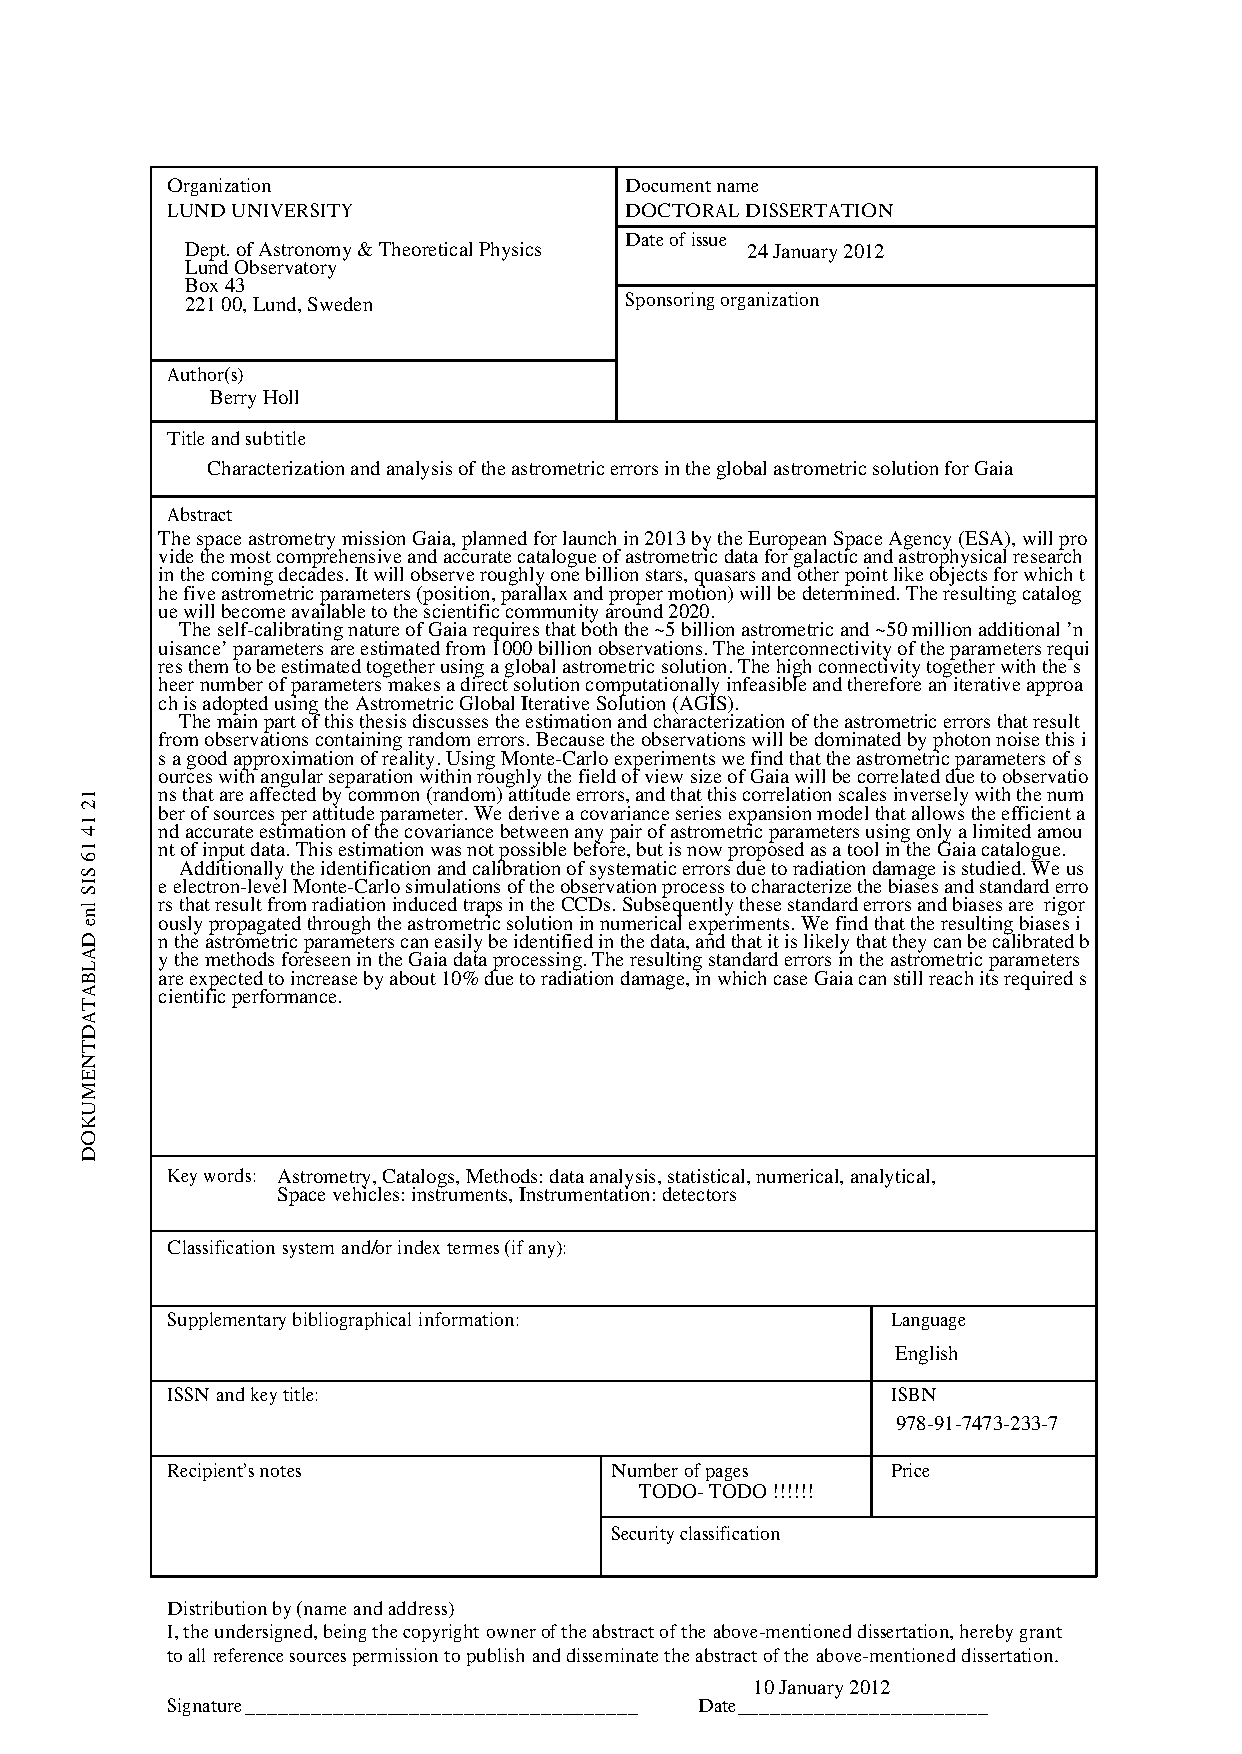
\includepdf[pages=1-1]{datasheetPDF_editable}

%%%%%%%%%%%%%%%%%%%%%%%%%%%%%%%%%%%%%%%%%%%%%%%%%%%%%%%%%%%%%%%%%%%%%%%
% Page five: title and author, without small text. Looks good!

\cleardoublepage
\thispagestyle{empty} % no page number
~
\vfill
\begin{center}
{\HUGE \myMainTitle}
\\[2mm]
{\huge \mySubTitle}

\vfill
{by \myName}

\vfill
% black and white (default):

\includegraphics[width=0.25\textwidth]{LundUniversity_C2line_BLACK.eps}

% Colour text in white so that the spacing is the same as on page three, but with less clutter
\color{white}{
\vspace{10mm}
{\large \myDegree}\\
{\large Thesis advisors: \myAdvisors}\\
{\large Faculty opponent: \myOpponent}\\
\vspace{1cm}
{\footnotesize
\myDefenceAnnouncement
}
}
\\
\end{center}
\vfill


%%%%%%%%%%%%%%%%%%%%%%%%%%%%%%%%%%%%%%%%%%%%%%%%%%%%%%%%%%%%%%%%%%%%%%%
% Page six: Cover image description, ISBN, copyright
\newpage 
\thispagestyle{empty} % no page number
%~
%\vfill
\vspace{-15mm}
A licentiate thesis at a university in Sweden takes either the form of a single,
cohesive research study (monograph) or a summary of research papers
(compilation thesis), which the licentiate student has written alone or together
with one or several other author(s). 

In the latter case the thesis consists of two parts. An introductory text puts
the research work into context and summarizes the main points of the papers.
Then, the research publications themselves are reproduced, together
with a description of the individual contributions of the authors. The
research papers may either have been already published or are manuscripts at
various stages (in press, submitted, or in draft). 

\vfill
{\small
\myCoverFront\\
\\
\myCoverBack\\
\\
\myFundingInformation


\vspace{5mm}
\copyright\, \myName~\myYear\\
\\
\myFaculty, {\myDepartment}
\\
\\
\ISBN: \myISBNprint~(print)\\ % ISBN av svenska ISBN centralen
\ISBN: \myISBNpdf~(pdf)\\ % ISBN av svenska ISBN centralen
%\mySeries\\
\\
Printed in Sweden by Media-Tryck, Lund~University, Lund~\myYear


\includegraphics[width=0.5\textwidth]{miljologotyper}
}


% ===============================================================
% ===================== INSPIRATIONAL QUOTE:  ===================
% ===============================================================
\newpage
\thispagestyle{empty} % No page number on quote page
~
\vspace{140pt}
\begin{flushright}
\textit{Dedicated to\\Humpty -- Dumpty\\bla bla blat}
\end{flushright}


\cleardoublepage


%%%%%%%%%%%%%%%%%%%%%%%%%%%%%%  Table of contents   %%%%%%%%%%%%%%%%%%%%%%%%%%%%%%%%%%%%%%%
\setcounter{page}{1} % Page Roman 1 of the frontmatter
\setcounter{tocdepth}{1}
\setcounter{secnumdepth}{2}
\tableofcontents
% no page number on toc page:
\addtocontents{toc}{\protect\thispagestyle{empty}}


%%%%%%%%%%%%%%%%%%%%%%%%%%%%%%%%% List of publications %%%%%%%%%%%%%%%%%%%%%%%%%%%%%%%%%%%%%%
% Have a long list and want to start on the left page? Here, have a special
% chapter heading for that!
%\addcontentsline{toc}{part}{Part 1: Summary}
%\renewcommand{\chapterheadstartvskip}{}
%{\let\cleardoublepage\relax \let\chapterheadstartvskip\nop 

\newpage
\sect{List of publications\label{sec:paperlist}}
This thesis is based on the following publications, referred to by their Roman numerals:
\vspace{2mm}

{
% Normal font size in this table, afterwards continue with slightly smaller table font size stated in preamble
\floatsetup[table]{font={normalsize},position=top}
\begin{tabularx}{\textwidth}{rX}
% Normal font size in this table, afterwards continue with slightly smaller table font size stated in preamble
\normalsize
\I	  & {\bf \PaperItitle}\\[2mm]
	  & \PaperIauthor\\
          & \PaperIref\\[6mm] 

\II	  & {\bf \PaperIItitle}\\[2mm]
	  & \PaperIIauthor\\
          & \PaperIIref\\[6mm]
\end{tabularx}

All papers are reproduced with permission of their respective publishers.
%Or maybe you need to be more specific? Like: Paper~I and II reproduced with permission \copyright\ ESO\\

% Publications not included in this thesis:
% \vspace{2mm}
%
% \begin{tabularx}{\textwidth}{rX}
% {\sc \phantom{vi}}   & {\bf \PaperNotIncItitle}\\[2mm]
%	  & \PaperNotIncIauthor\\
%          & \PaperNotIncIref\\[5mm] 
%
%\end{tabularx}
%
} % End large font tables, continue with font size stated in preamble


                 
% ===============================================================
% ====================== Acknowledgements:  =====================
\newpage
\sect{Acknowledgements}
\blindtext

% ===============================================================
% ===================== POPULAR SUMMARIES:  =====================

%----------------- SUMMARY IN SWEDISH --------------------
\newpage
\selectlanguage{swedish}
\sect{Populärvetenskaplig sammanfattning på svenska}
\blindtext

% ===============================================================
% ======================= SUMMARY CHAPTER   =====================
% Back to British spelling
\selectlanguage{english}
% Need to add hyphenation corrections? Do like this:
% \hyphenation{as-tro-me-try ana-lysis}

% Page numbers arabic 
\mainmatter
% Reset table counters to not count the publications table
\setcounter{table}{0} 
% Rest page counters, this is where it all starts!
\setcounter{page}{1}

\chap{\myTitle}
% Fancy a quote?
\newpage

%%%%%%%%%%%%%%%%%%%%%%%%%%%%%%%%%%%%%%%%% Actual kappa %%%%%%%%%%%%%%%%%%%%%%%%%%%%%%%%%%%%%%%%%
%\part{Research motivation}
\part{Fundamental theory}
\chapter{Introduction to quantum chromodynamics}
\def \imgpath {"./figures/intro"}

This chapter serves as an introduction to particle physics, QCD, and phenomenology of high energy QCD interactions, with the focus on multiple partonic interactions and string formations. Furthermore, it introduces the physics of QCD matter and the deconfinement of hadrons.

\section{Standard Model of elementary particles}

The Standard Model (SM) of particle physics is a set of theories describes \textit{elementary} constituents of matter and their interactions via fundamental forces of the Universe. It has been formulated in the 1970s, combining frameworks of quantum field theory (QFT), gauge symmetries, and spontaneous symmetry breaking.

Matter particles in the SM are classified into two main categories: quarks and leptons. Quarks come in six flavours (\textit{up, down, charm, strange, top, and bottom}) and form hadrons, i.e.\ \textit{baryons} ($qqq$) and \textit{mesons} ($q\bar{q}$). The lepton sector also comprises six flavours (\textit{electron, muon, tau, and their corresponding neutrinos}). Quarks and leptons are fermions with an intrinsic spin $1/2$. Furthermore, matter particles in the SM also come with associated antiparticles, which have opposite quantum numbers but the same mass.

The interactions between matter particles in the SM are mediated by an exchange of gauge bosons. There are three fundamental forces in the SM, described by four types of vector bosons (ordered by their typical strength): 
\begin{enumerate}
\item \textit{Strong force}, mediated by the gluon.
\item \textit{Electromagnetic force}, mediated by the photon.
\item \textit{Weak force}, mediated by the massive bosons $W^\pm$ and $Z^0$.
\end{enumerate} 

Moreover, the interactions are associated with local gauge symmetries, which determine their mathematical structure. The symmetry group for the SM is SU($3$)$\times$SU($2$)$\times$U($1$), corresponding to the strong and the electroweak sector. \cite{tanabashiReviewParticlePhysics2018}

In addition, the SM also includes the scalar Higgs boson, which is responsible for giving mass to other elementary particles. This is achieved via the Higgs mechanism \cite{higgsBrokenSymmetriesMasses1964, englertBrokenSymmetryMass1964}, which involves the spontaneous breaking of the electroweak symmetry in the early universe. The Higgs boson was discovered experimentally at the Large Hadron Collider (LHC) in 2012 by the ATLAS \cite{theatlascollaborationObservationNewParticle2012} and CMS \cite{thecmscollaborationObservationNewBoson2012} collaborations, confirming a key prediction of the SM.

Nevertheless, the SM has several limitations, including its inability to account for dark matter, explain why the particle masses span over several orders of magnitude, and the CP violation problem related to the observed matter-antimatter asymmetry in the Universe. These are actively investigated in Beyond Standard Model (BSM) theories.

\begin{figure}[H]
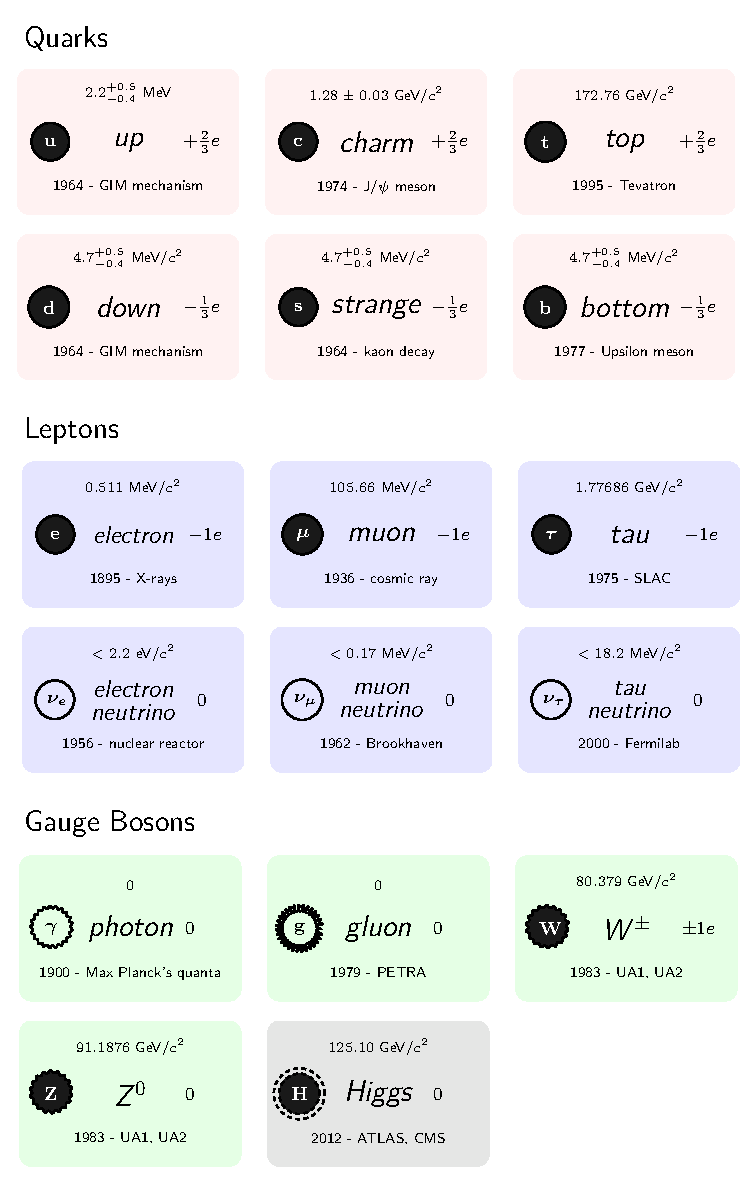
\includegraphics[width=0.90\textwidth]{\imgpath/SM.pdf}
\caption{Particle of the Standard Model, listed together with their mass, electric charge, and the  year and means of discovery (going clockwise from the top). VALUES NEED TO BE FIXED.}
\end{figure}

\section{Coordinate systems and kinematic observables}

Particles in HEP processes are described by their Lorentz-invariant four-vectors, $\bm{x} = (ct, x, y, z)$ and $\bm{p} = (E/c, p_x, p_y, p_z) = (E/c, \vec{\pt} , p_z)$, where $|\vec{\pt}| \equiv \sqrt{p_x^2+p_y^2}$. In LHC experiments, the coordinate system is defined such that the $x$-axis points in the direction of the centre of the LHC, and the $z$-axis points in the direction of the beam, as shown in Fig.~\ref{fig:intro:coordinates}. In addition to the standard Cartesian coordinates, two observables, $\varphi$ (azimuthal angle) and $\eta$ (pseudorapidity), are used to describe the position and momentum of particles relative to the interaction point, which is located at $x = y = z = 0$. Pseudorapidity is defined as a function of the polar angle $\theta$, where 
\begin{align}
\eta = -\ln(\tan(\theta/2)) \quad .
\end{align}
For high-momentum particles ($E \simeq pc$), pseudorapidity is an approximation of the rapidity relative to the beam, given by 
\begin{align}
y = \frac{1}{2} \ln \frac{E + p_z c}{E - p_z c} \quad .
\end{align}
Rapidity is a convenient quantity to use because it transforms additively under Lorentz boosts, unlike velocity. In these coordinates, the following relations hold:
\begin{align}
p_x = |\vec{\pt}| \cos \varphi \, , \quad \
p_y = |\vec{\pt}| \sin \varphi \, , \quad \
p_z = |\vec{p} \,| \sinh \eta \, .
\end{align}

\begin{figure}[H]
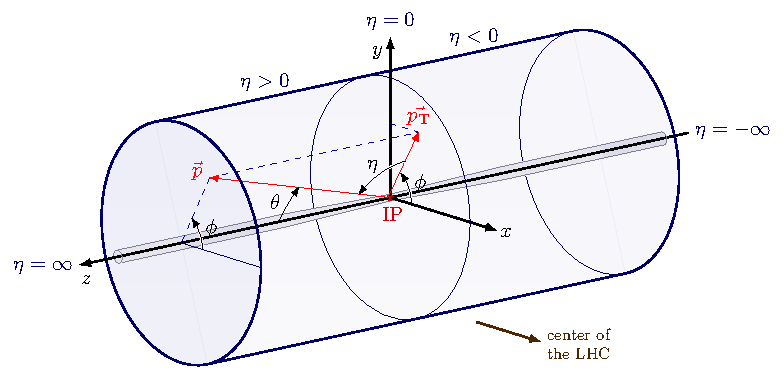
\includegraphics[width=0.85\textwidth]{\imgpath/coordinates.pdf}
\caption{Coordinate system of an LHC experiment, with the interaction point in the centre.}
\label{fig:intro:coordinates}
\end{figure}

\section{Quantum electrodynamics, electrons, and photons}

In many aspects, QCD is a very similar theory to the simpler and better explored theory QED. In QFT, dynamics of particles can be provided in terms of its Lagrangian density $\mathcal{L}$, from which equations of motions can be derived and which is also used to calculate interaction probabilites. The QED theory with a local U($1$) symmetry has its $\mathcal{L}_\mathrm{QED}$ defined as:

\begin{equation}
\mathcal{L}_\mathrm{QED} = \bar{\psi}(i \slashed \partial - m)\psi - \frac{1}{4}F_{\mu\nu}F^{\mu\nu} - e\bar{\psi}\slashed A \psi \quad ,
\end{equation}
where $\psi$ is the electron field with mass $m$ and electric charge $e$, $F_{\mu\nu}$ the electromagnetic field-strength tensor, and Feynman slash notation is employed. The first part describes the dynamics of the electron fields, the second part describes the dynamics of the electromagnetic field, and the last part describes the interaction of electrons and photons with a coupling strength $e$. Using Feynman diagrams, they can be visualised as:
\begin{figure}[H]
\adjustbox{valign=m}{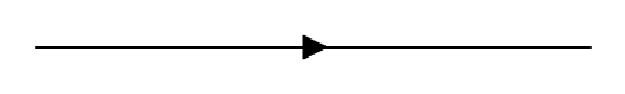
\includegraphics[width=0.19\textwidth]{\imgpath/qed1.pdf}}\hspace{1em}
\adjustbox{valign=m}{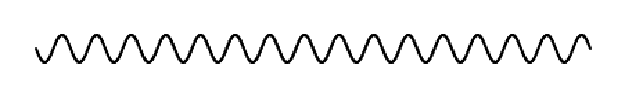
\includegraphics[width=0.19\textwidth]{\imgpath/qed2.pdf}}\hspace{1em}
\adjustbox{valign=m}{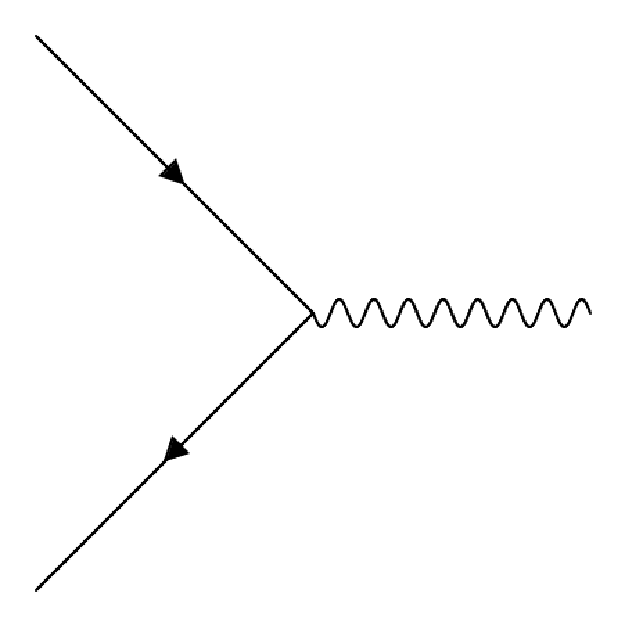
\includegraphics[width=0.19\textwidth]{\imgpath/qed3.pdf}}
\end{figure}

In QED interactions, each vertex depicted in the Feynman diagrams contributes to the probability of the process with a coefficient $\alpha$ (to the matrix elements as $\sqrt{\alpha}$, which is the coupling constant defined as $\alpha = e^2/4\pi$. This constant is generally small, which allows for interactions to be calculated using perturbation theory as an expansion series in $\alpha$. The contributions to the series correspond to different Feynman diagrams representing the possible interaction processes, and they are ordered in powers of $\alpha$ based on the complexity of the diagrams.

Contributions from higher orders, such as the electron loop depicted below, lead to ``screening" of the effective charge at large distances/small momenta, which makes the coupling constant dependent on the scale of the process $\mu$. For example, at low energies corresponding to atomic scales, $\alpha \approx 1/137$, but at scales of the $Z^0$ boson mass, $\alpha \approx 1/127$ \cite{fritzschFundamentalConstantsHigh2002}. The \textit{running} of this coupling is given by the $\beta$ function, $\beta(\alpha) \equiv \frac{\partial \alpha}{\partial \log \mu^2}$, and it can be calculated by quantifying the effective coupling strengths at various orders of perturbation theory and using renormalisation group tools \cite{delamotteHintRenormalization2004}, although renormalisation is a more general concept. In QED, the screening leads to a positive sign in $\beta$ calculated at lowest order, which means that when solving for $\alpha$ by integrating, $\alpha$ grows with energy scale\footnote{The scale at which QED eventually breaks down due to this increase is well above the Plack mass.}.

\begin{figure}[H]
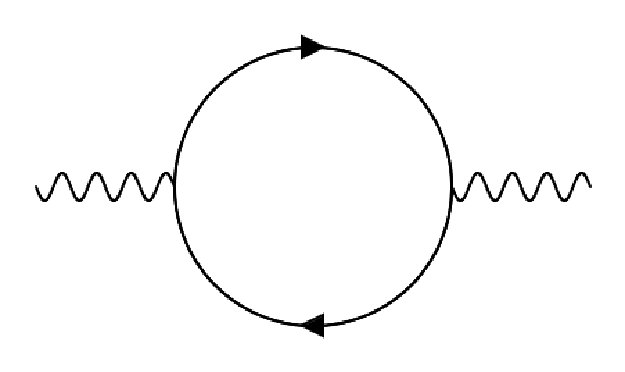
\includegraphics[width=.26\textwidth]{\imgpath/qedloop.pdf}
\end{figure}

Renormalisation is also used when calculating physical quantities where loop contributions lead to divergences, which are then absorbed into the parameters of the theory. The success of these procedures and the QED theory as a whole is validated by excellent prediction power for experimental measurements, such as the magnetic moment of an electron \cite{odomNewMeasurementElectron2006}.

\section{Quantum chromodynamics, quarks, and gluons}

In QCD, particles have an additional quantum number called colour charge: red, green, and blue. Thus, there are three quarks of each flavour and eight gluons mediating interactions between. Gluons also carry colour charges, which allows them to interact with each other, making the theory non-Abelian. The QCD Lagrangian is symmetric under local SU($3$) transformations and takes the shape of:

\begin{align}\label{eq:intro:lqcd}
\mathcal{L}_\mathrm{QCD} &= \sum_{f}^{n_f} \bar{\psi}_i^{(f)}(i \slashed D_{ij}-m_f \delta_{ij} ) \psi_j^{(f)} \, - \frac{1}{4} \sum_a^8 F^{\mu\nu}_a F_{\mu\nu}^a \quad , \\
D^\mu_{ij} &\equiv \partial^\mu \delta_{ij} + i g_s t^a_{ij}A^\mu_a \quad , \\
F^a_{\mu\nu} &\equiv \partial_\mu A^a_\nu - \partial_\nu A^a_\mu - g_s f_{abc} A^b_\mu A^c_\nu \quad ,
\end{align}
where $\psi$ are the quark fields of $n_f$ different flavours with mass $m_f$ and colour $i,j$, $D^\mu_{ij}$ the covariant derivative with the coupling strength $g_s$ and eight SU($3$) generators given by matrices $t^a_{ij}$, and $A_a^{\mu}$ are the gluon fields \cite{altarelliQCDPrimer2002}. Lastly, $F^a_{\mu\nu}$ is the field-strength tensor with $f_{abc}$ being structure constants. The Lagrangian now also contains terms with interactions between gluons. In the representation of Feynman diagrams, for the interactions, there is:
\begin{figure}[H]
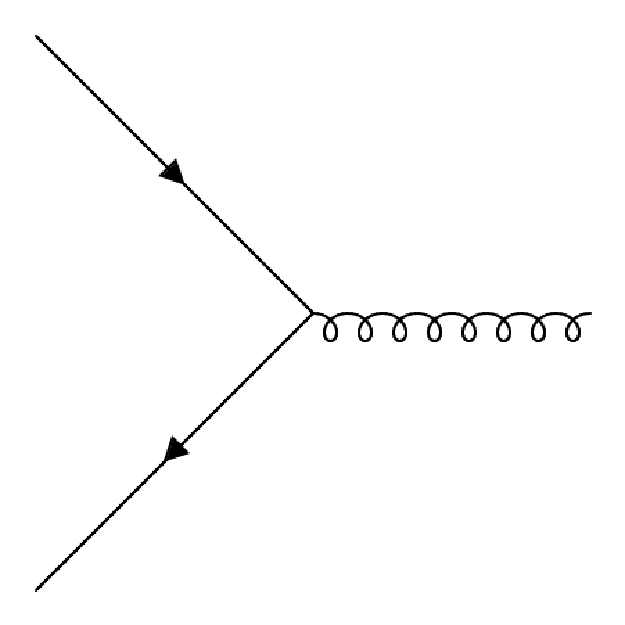
\includegraphics[width=0.19\textwidth]{\imgpath/qcd3.pdf}\hspace{1em}
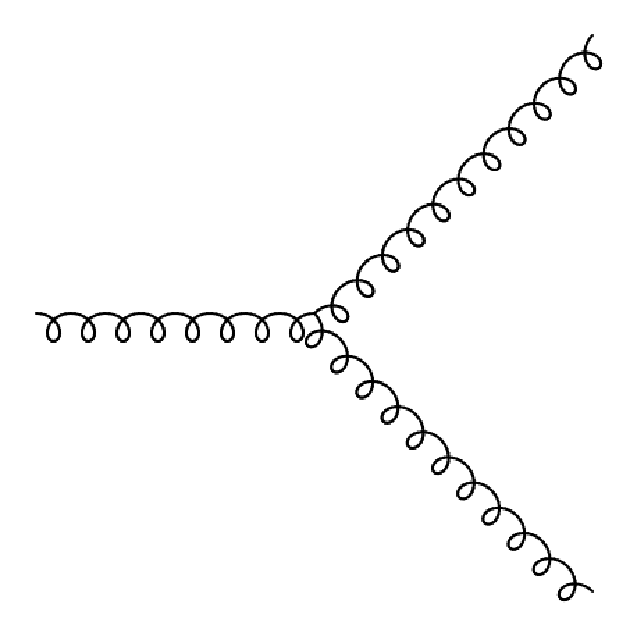
\includegraphics[width=0.19\textwidth]{\imgpath/qcd4.pdf}\hspace{1em}
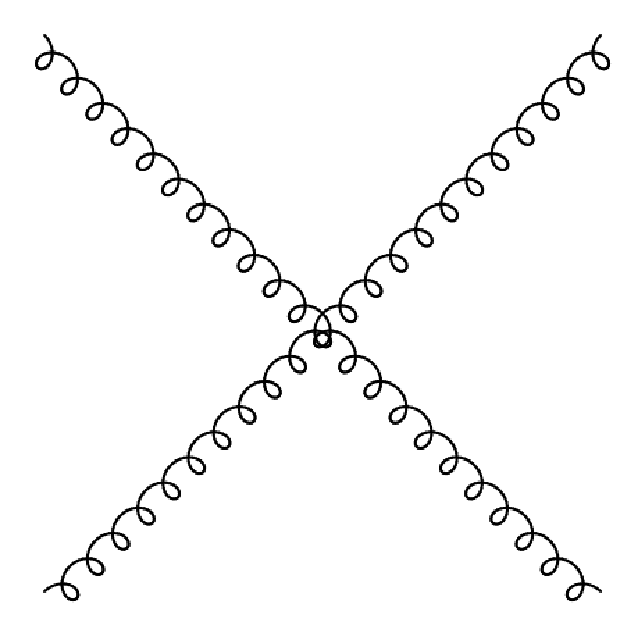
\includegraphics[width=0.19\textwidth]{\imgpath/qcd5.pdf}
\end{figure}

Similarly to the QED case, the strong coupling constant can be defined as $\alpha_s = g^2/4\pi$. However, when considering its modifications due to virtual corrections, in addition to the quark loop, there is also a gluon loop.:
\begin{figure}[H]
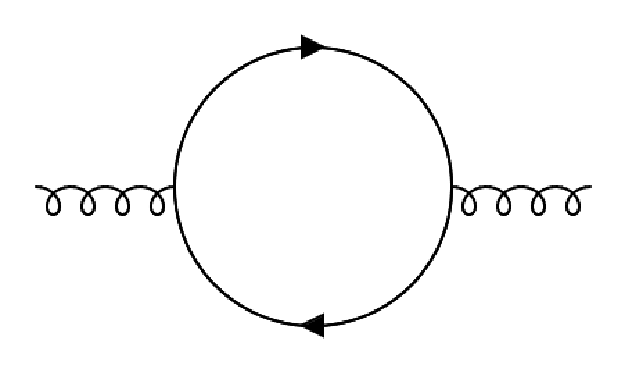
\includegraphics[width=0.26\textwidth]{\imgpath/qcdloop1.pdf}\hspace{2em}
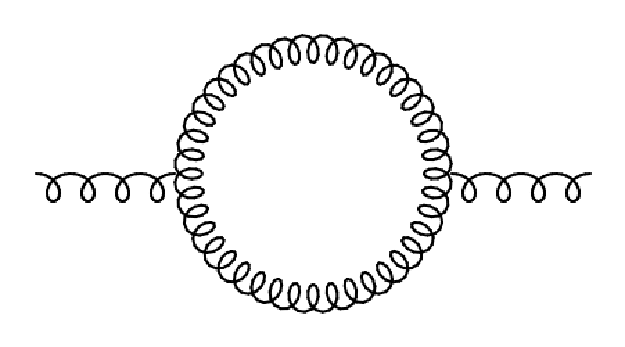
\includegraphics[width=0.26\textwidth]{\imgpath/qcdloop2.pdf}
\end{figure}

The gluon loop contributes to the $\beta$ function in an opposite and larger way than the quark loop, and so overall, there is an \textit{anti-screening} effect instead and a negative sign in the calculated one-loop $\beta$ function. The running of the coupling can be calculated as:
\begin{align}
\alpha_s (\mu) = \frac{1}{b_0 \log ( \mu^2 / \Lambda_\mathrm{QCD}^2 )} \quad ,
\end{align} 
where $b_0$ is a constant computed from the loop calculations, $b_0 = \frac{11-\frac{2}{3}n_f}{4\pi}$ \cite{politzerReliablePerturbativeResults1973}. The introduced $\Lambda_\mathrm{QCD}$ is a scale parameter of the theory corresponding to the energy where the coupling becomes infinite, and depends on the definition of $\alpha_s$ and the number of available quark flavours $n_f$ \cite{altarelliQCDPrimer2002}. It ranges between $200$ and $\mevcc{300}$ \cite{deurQCDRunningCoupling2016}.

From the running, it is evident that the coupling strength decreases with increasing energy, which is known as \textit{asymptotic freedom} \cite{politzerReliablePerturbativeResults1973,grossAsymptoticallyFreeGauge1973} and corresponds to the fact that strong interaction is short-ranged. On the other hand, at low values, $\alpha_s$ diverges, which is related to the fact that quarks are bound to hadrons -- \textit{quark confinement}. The evolution of $\alpha_s$ also limits the applicability of perturbation theory at low energy regimes; calculations from perturbative QCD (pQCD) are relevant at leading orders starting typically from $1-\gevcc{2}$. The measured $\alpha_s(\mu)$ is shown in Fig.~\ref{fig:intro:alpha}, and at scales of the $Z^0$ boson mass is approximately $0.1185 \pm 0.0006$ \cite{dissertoriDeterminationStrongCoupling2016, particledatagroupReviewParticlePhysics2022}.

\begin{figure}[H]
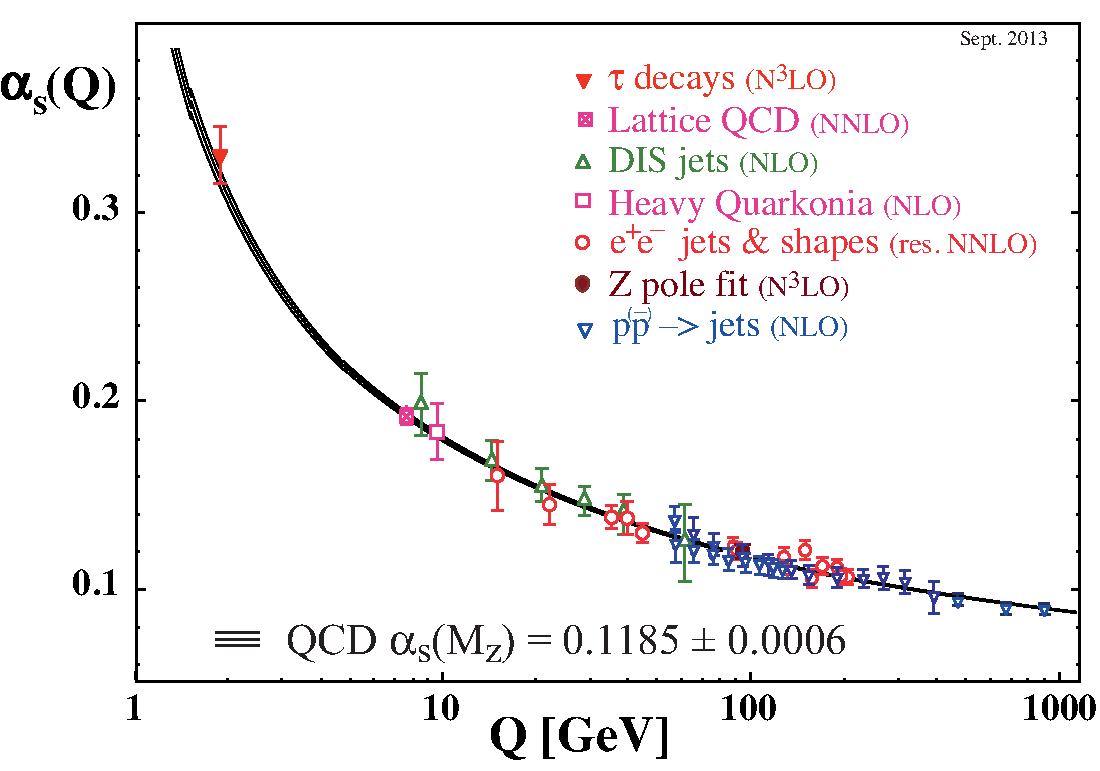
\includegraphics[width=0.55\textwidth]{\imgpath/alpha.pdf}
\caption{Strong coupling constant determined at different energy scales through various measurements and numerical calculations (data points) and compared with theoretical predictions from QCD. \cite{dissertoriDeterminationStrongCoupling2016}}
\label{fig:intro:alpha}
\end{figure}

\section{From partons to hadrons}

\subsection{Initial and Final State Radiation}

In QFT, charged particles are surrounded by a cloud of virtual particles, which can be thought of as fluctuations in the particle's field. For example, the electron state can be described as a superposition of the bare electron plus additional massless bosons:
\begin{align}
|\mathrm{e}\rangle_\mathrm{phys} = |\mathrm{e}\rangle + |\mathrm{e}\gamma\rangle + |\mathrm{e}\gamma\gamma\rangle + \ldots
\end{align}
and, at higher orders, pairs of virtual electrons. The fluctuations continuously form and recombine, with their lifetime depending on their energy and momentum. Specifically, the lifetime of a fluctuation with energy $\omega$ and transverse momentum $k_\mathrm{T}$ can be approximated as:
\begin{align}
\tau \approx \frac{\omega}{k_\mathrm{T}} \quad .
\end{align}
This implies that fluctuations with smaller-$k_\mathrm{T}$ live longer. \cite{prestelParticlePhysicsPhenomenology}

As illustrated in Fig.~\ref{fig:intro:isrfsrsketch}, the coherent mixed state of the bare charge and the field fluctuations can be disturbed by the presence of an interaction. Intuitively, this interaction can change the energy and momentum of the fluctuations, their formation and recombination, and lead to the emission of radiation in two ways:
\begin{enumerate}
\item a fluctuation is kicked on-shell by the interaction and part of the field continues in its original direction, which leads to Initial State Radiation (ISR);
\item as a result of the field of the scattered particle rearranging itself , which can be a source of Final State Radiation (FSR).
\end{enumerate}

In both of the cases, a larger momentum transfer implies more radiation. \textit{For hard, wide angle emissions, cross sections can be calculated perturbatively at fixed orders}. 

Soft and collinear emissions, however, lead to infra-red divergences ($\propto \frac{1}{\omega}$,$\propto \frac{1}{k_\mathrm{T}^2}$) and thus, need to be factorised away from the amplitudes or the cross sections and then described using resummation techniques. Without any emissions, the probabilities of finding electrons and photons of fractional momentum $x$ with respect to the whole system are:
\begin{align}
f_\mathrm{e} (x) = \delta (1-x) \, , \quad \ f_\gamma(x) = 0 \, ,
\end{align}
When considering the emissions above some scales parametrised by the resolution parameter $Q^2$, these probabilities, however, evolve according to the DGLAP equation \cite{altarelliAsymptoticFreedomParton1977} :
\begin{align}
\label{eq:intro:dglap}
\frac{\partial}{\partial\ln Q^2}
\begin{pmatrix}
f_e(x, Q^2)\\
f_{\gamma}(x, Q^2)
\end{pmatrix}
&= \frac{\alpha_\mathrm{em}}{2\pi}
\int_x^1 \frac{dz}{z}
\begin{pmatrix}
P_{ee}(z) & P_{e\gamma}(z)\\
P_{\gamma e}(z) & P_{\gamma\gamma}(z)
\end{pmatrix}
\begin{pmatrix}
f_e\left(\frac{x}{z}, Q^2\right)\\
f_{\gamma}\left(\frac{x}{z}, Q^2\right)
\end{pmatrix} \quad ,
\end{align}
where $P_{ij}(z)$ are the splitting probability functions of a particle $i$ emitting a particle $j$.

In QCD, the behaviour is analogous, with $\alpha_\mathrm{em} \rightarrow \alpha_s$, $e\rightarrow q$, and $\gamma \rightarrow g$. \cite{prestelParticlePhysicsPhenomenology}

\begin{figure}[H]
\subfloat[][]{\adjustbox{valign=m}{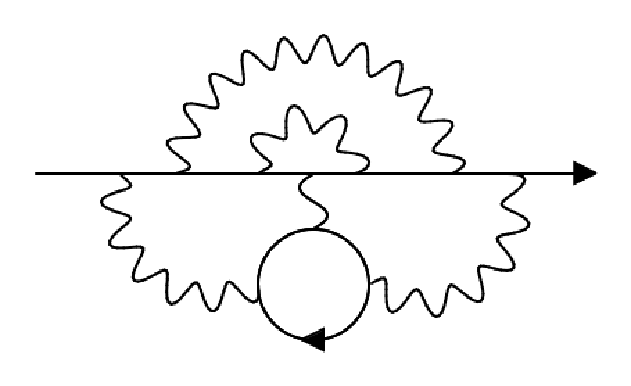
\includegraphics[width=.240\textwidth]{\imgpath/eisr1.pdf}}\adjustbox{valign=m}{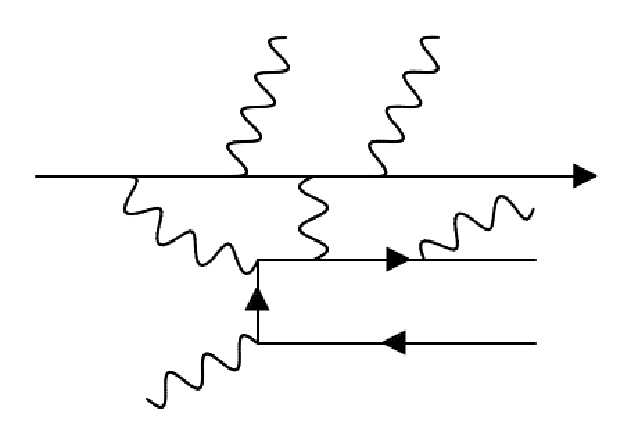
\includegraphics[width=.240\textwidth]{\imgpath/eisr22.pdf}}}
\subfloat[][]{\adjustbox{valign=m}{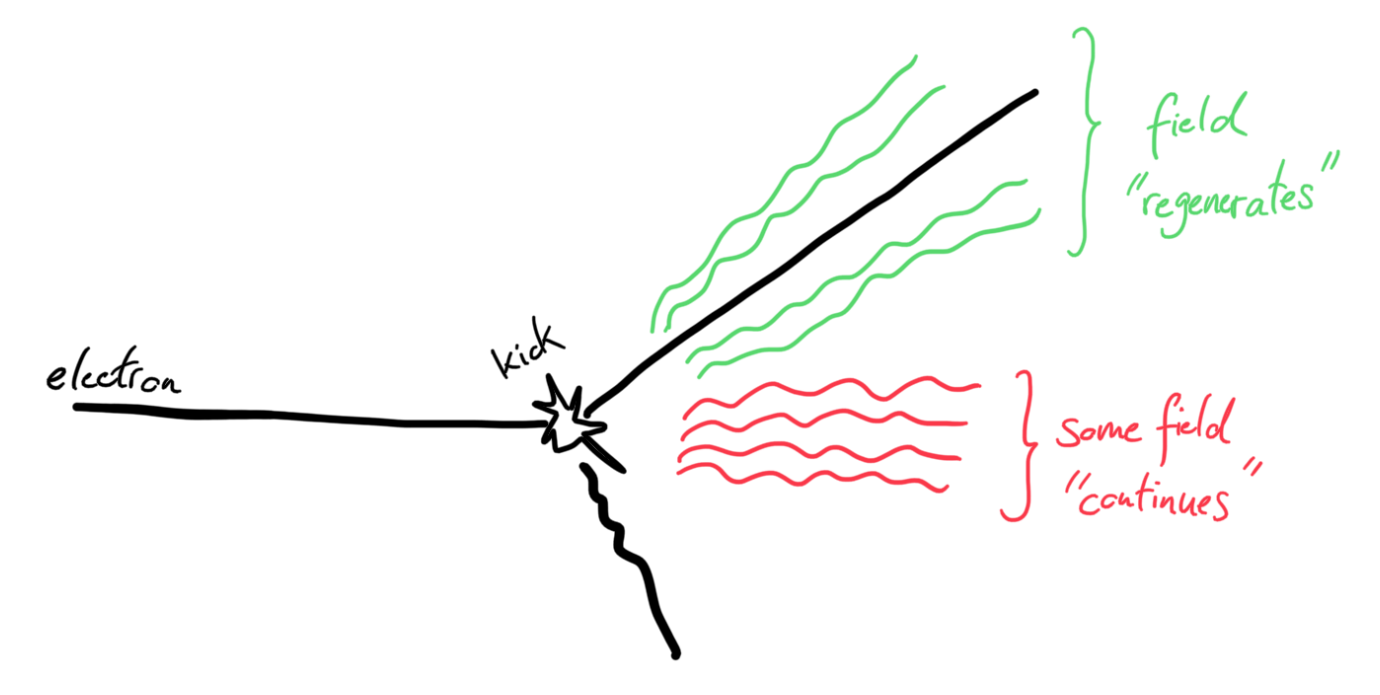
\includegraphics[width=.480\textwidth]{\imgpath/isrfsr2.png}}}
\caption{\textbf{(a)} Illustration of the field fluctuations before and after the state coherence gets disturbed by an external actor. \textbf{(b)} Illustration of emmisions of radiation in a scattering process.}
\label{fig:intro:isrfsrsketch}
\end{figure}

\subsection{Factorisation theorem}

The evolution equation (\ref{eq:intro:dglap}) implies that the probabilities of observing emissions with a fractional momentum $x$ depend on the resolution $Q^2$. In QCD, 
\begin{enumerate}
\item when applied to the initial state, they are known as parton distribution functions (PDFs) and determine the probabilities of finding partons\footnote{Partons refer to the valence quarks, sea quarks, and gluons inside hadrons.} in the composite hadronic state. 
\item When applied to the final state, they are called fragmentation functions, and determine the probabilities of measuring fragments of the outgoing particles.
\end{enumerate}

This leads to the factorisation theorem \cite{collinsFactorizationHardProcesses2004} for processes involving collisions of two hadrons, which separates the perturbatively calculable partonic cross section from the non-perturbative partonic evolution and hadronisation. The theorem can be expressed as follows:
\begin{align}\label{eq:intro:facto}
\sigma = f_i^A(x_i,\mu_F)f_j^B(x_j,\mu_F) \otimes \hat{\sigma}_{ij\to n}(\mu_F,\mu_R) \otimes D_{n \to n'} \, .
\end{align}
Here, $i$ and $j$ are the initial partons, $\hat{\sigma}_{ij\to n}$ is the partonic cross section, $D_{n \to n'}$ is the process-specific fragmentation function for evolving the partons $n$ into the particles' final state $n'$, and $\mu_F$ and $\mu_R$ are the factorisation and renormalisation scales, respectively. The factorisation scale, $\mu_F$, determines the scale below which the emissions are absorbed into the PDFs. The theorem is depicted in Fig.~\ref{fig:intro:factorisation}.

\begin{figure}[H]
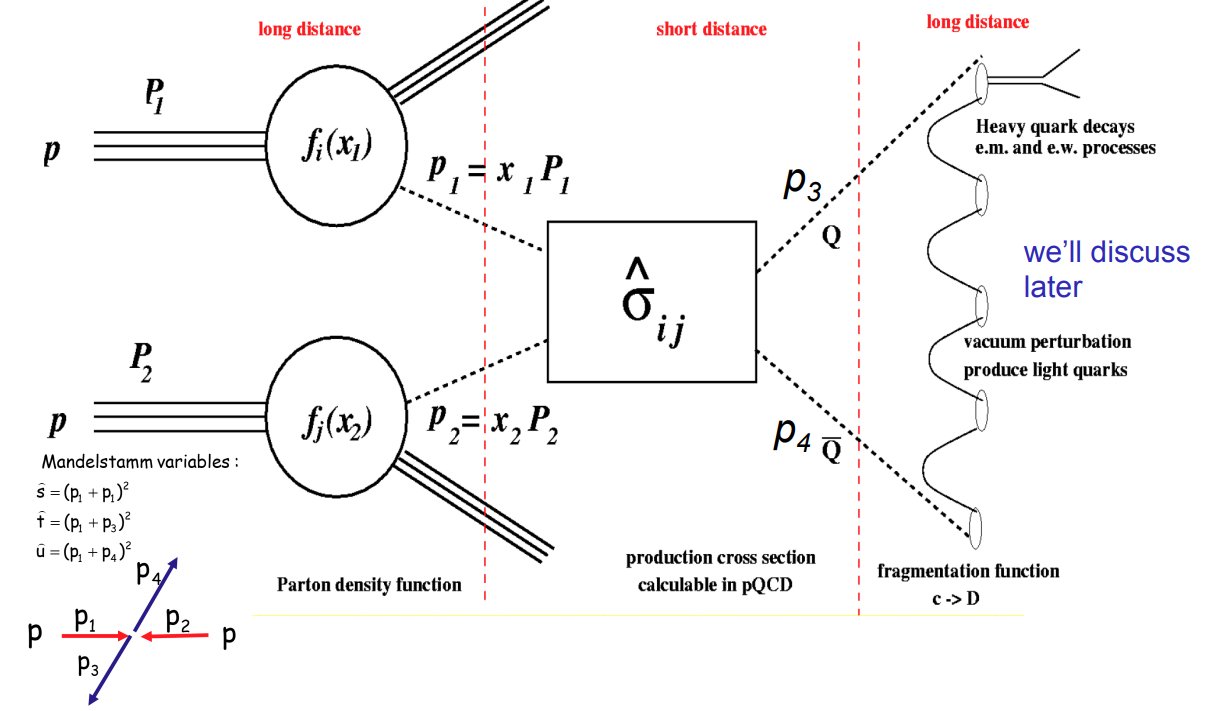
\includegraphics[width=0.65\textwidth]{\imgpath/factorisation.png}
\caption{Illustration of the factorisation theorem. (NEEDS TO BE REMADE).}
\label{fig:intro:factorisation}
\end{figure}

\subsection{Parton distribution functions}

The PDFs defining the probabilities of finding quarks and gluons in nucleons can be determined experimentally at hadron-electron colliders such as HERA \cite{cooper-sarkarExtractionProtonParton2008}. They are determined from measurements of deep inelastic scatterings in a range of energies and momentum transfers. They are displayed in Fig.~\ref{fig:intro:pdfs} as a function of the fractional momentum $x$ (also called Bj\"orken $x$). 

According to collider kinematics, $x \propto \frac{1}{\sqrt{s}e^y}$, therefore, the partonic composition of ultra-relativistic hadrons is dominated by gluons. Following unitarity principles and BK evolution equation \cite{marquetBalitskyKovchegovEquationFull2005}, it is expected that gluons start recombining and the gluonic content saturates as $x\rightarrow0$. This is actively reseached \cite{starcollaborationEvidenceNonlinearGluon2022}, however, not directly measured yet. Additionally, it should be noted that in ultra-relativistic heavy nuclei, the partons are modified in the contracted nuclear environment and the PDFs are referred to as nPDFs.

\begin{figure}[H]
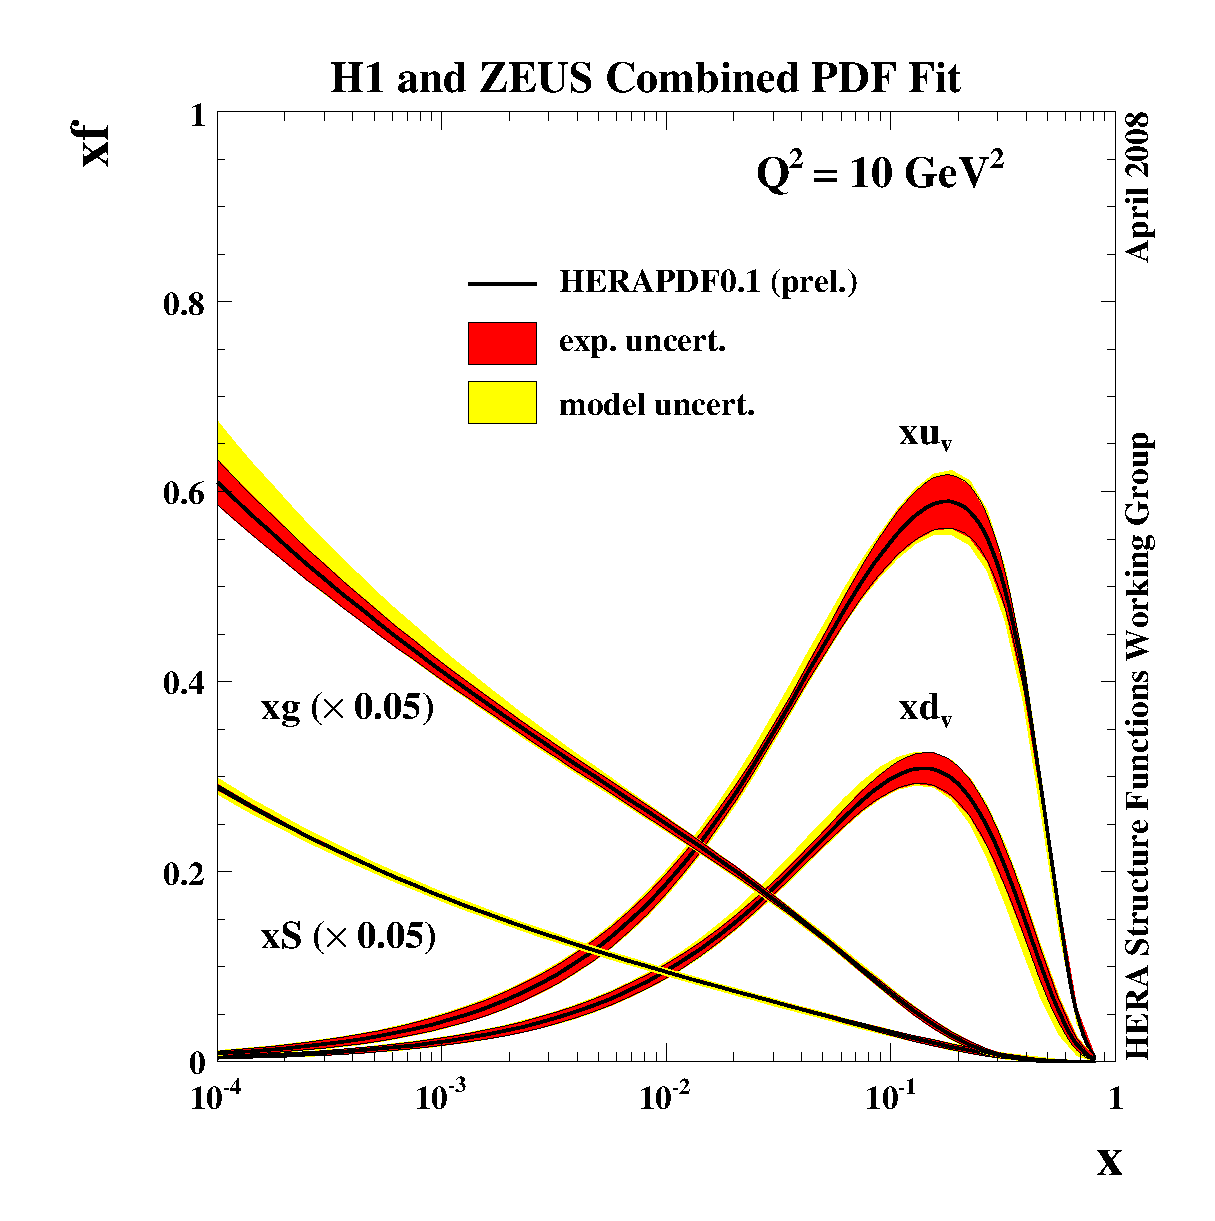
\includegraphics[width=0.4\textwidth]{\imgpath/pdf.eps}
\caption{Parton distribution functions determined in ep scatterings at HERA as a function of the fractional momentum for the up, down, sea quarks, and gluons. \cite{cooper-sarkarExtractionProtonParton2008}}
\label{fig:intro:pdfs}
\end{figure}

\subsection{Parton fragmentation and the Lund string}

After the scattering process, the produced partons continue to fragment by emitting more partons in a process called the parton shower. Since the coupling strength in QCD increases with decreasing the energy scale of the splitting, this leads to the production of many soft, collimated emissions known as jets. The partonic evolution continues until the virtuality of the partons reaches the hadronization scale ($\approx \Lambda_\mathrm{QCD}$). There are multiple frameworks within QCD to describe the evolution of partons into their final state, such as using the DGLAP equations or the so-called dipole formalism.

Once the partonic final state is reached, the partons hadronise into the observable mesons and baryons. The hadronisation process is not calculable in QCD and requires phenomenological models to describe it. One such model is the Lund string model \cite{ferreres-soleSpaceTimeStructureHadronization2018}, which describes hadronisation as the breaking of a color string between the quarks in the final state. In this model, the energy stored in the color string is converted into the mass of new hadrons.

According to confinement, hadronisation should involve at least two partons with complementary colours. In QCD, the $q\bar{q}$ potential takes the shape of
\begin{align}\label{eq:intro:qqpot}
V_{q\bar{q}} \approx - \frac{4}{3}\frac{\alpha_s \hbar c}{r} + \kappa r \quad ,
\end{align}
where $\kappa$ is a parameter with value around $1 \mathrm{GeV} /\mathrm{fm}$. In the non-perturbative regime (long distances), the potential is dominated by the linear part, which is reminiscent of a system bound by a string with tension $\kappa$. This is taken advantage of by the Lund string model -- a $q$ and $\bar{q}$ pair separated by distance $\Delta x$ is bound by a color field (string) with energy $\kappa \Delta x$. 

If the $q$ and $\bar{q}$ continue separating as a result of the scattering, the energy stored in the color field increases. At some point, it can become energetically favourable to produce a new $q\bar{q}$ pair out of vacuum, which is a quantum mechanics tunnelling phenomenon characterised by the probability:
\begin{align}
\frac{\mathrm{d}P}{\mathrm{d}m_\mathrm{T}} \propto \exp \left( -\frac{\pi m_\mathrm{T}^2}{\kappa} \right) \quad ,
\label{eq:intro:tunnel}
\end{align}
where $m_\mathrm{T}$ is the transverse mass of the produced quarks. Otherwise, the $q\bar{q}$ system starts contracting and oscillates with a period $T = 2 E_\mathrm{kin}/\kappa$, where $E_\mathrm{kin}$ is its maximum kinetic energy. The produced $q$ and $\bar{q}$ then connect by new color fields to the original pair. This process repeats itself resulting in a cascade of many $q\bar{q}$ pairs connected by many color strings. In this description, baryons can also be created by double tunnelling of a $qq\overline{qq}$ pair. The process is illustrated in Fig.~\ref{fig:intro:lundstring}.

\begin{figure}[H]
\subfloat[][]{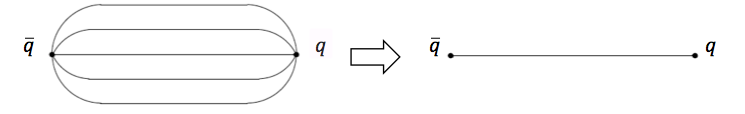
\includegraphics[width=.330\textwidth]{\imgpath/tubelike.png}}
\subfloat[][]{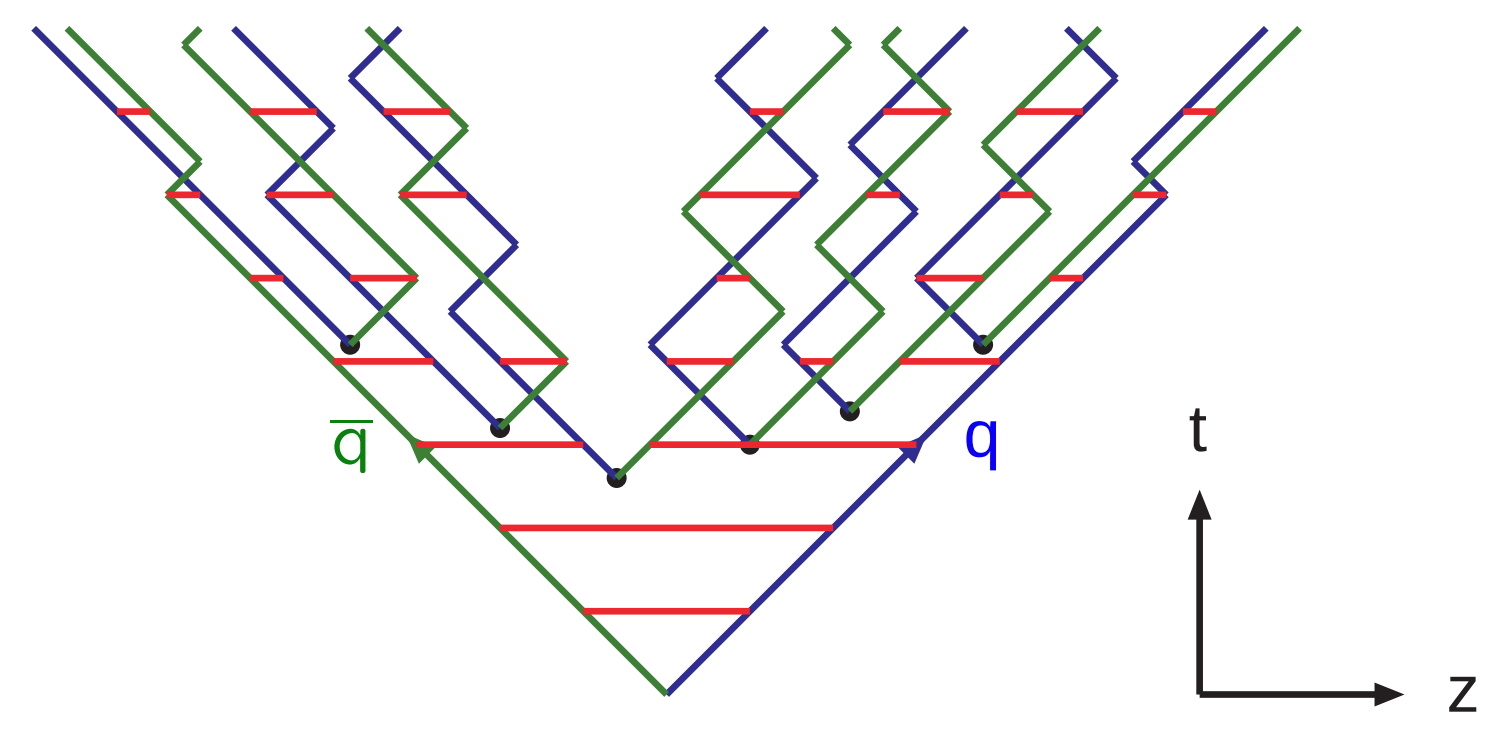
\includegraphics[width=.330\textwidth]{\imgpath/lundstring.png}}
\subfloat[][]{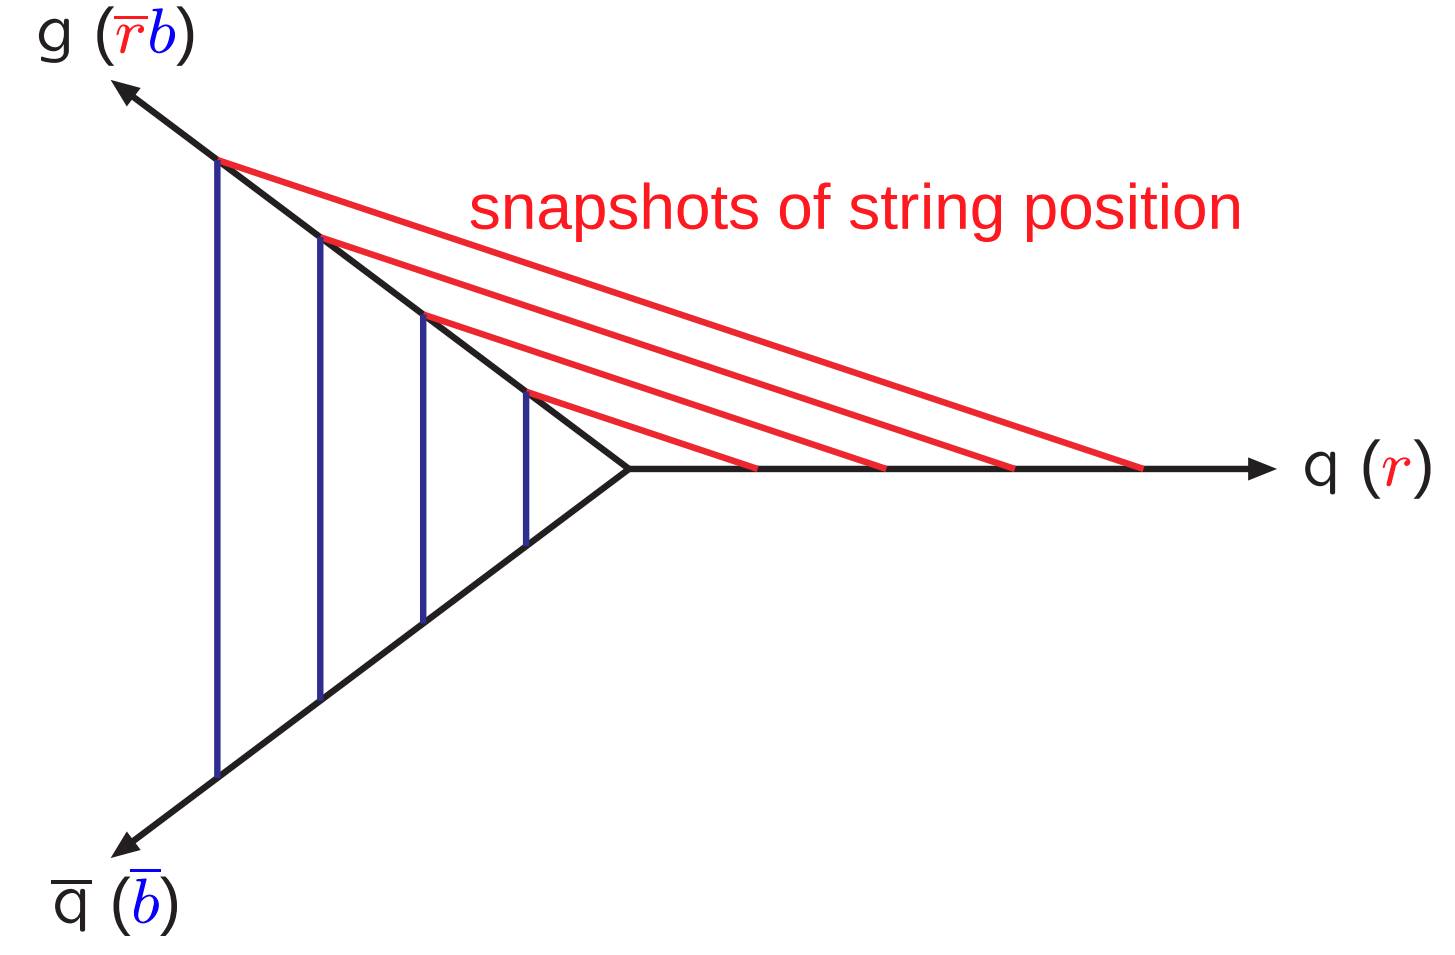
\includegraphics[width=.330\textwidth]{\imgpath/lundgluon.png}}
\caption{\textbf{(a)} Illustration of the color field between two quarks and its simplified representation with a string  \cite{ferreres-soleSpaceTimeStructureHadronization2018}. \textbf{(b)} Illustration of the string splitting by producing new $q\bar{q}$ in the $t-z$ plane \cite{ferreres-soleSpaceTimeStructureHadronization2018}. \textbf{(c)} Visualisation of the treatment of gluons in the Lund string model \cite{sjostrandQCDBSMPYTHIA2011}.}
\label{fig:intro:lundstring}
\end{figure}

Equation \ref{eq:intro:tunnel} also implies that production of strange quarks is suppressed by a factor of 
\begin{align}\label{eq:intro:rho}
\rho = \exp \left( -\frac{\pi (m^2_s - m^2_{u,d})}{\kappa} \right) \quad .
\end{align}
This parameter is typically tuned to data, as substituting constituent ($m_s \approx \gevcc{0.5}$, $m_{u,d} \approx \gevcc{0.33}$) versus current masses ($m_s \approx \gevcc{0.1}$, $m_{u,d} \approx 0$) leads to considerable differences underestimating and overestimating data, respectively.

For a $q\bar{q}g$ system, in this model, the gluon connects to the quark and antiquark and is effectively treated as a ``kink" on the color field, adding energy and momentum to the $q\bar{q}$ string (stretching it in its direction), as visualised in Fig.~\ref{fig:intro:lundstring}.

It should be noted that in the paradigm of AA collisions, hadron production can be alternatively modelled by hadronisation at the QGP's phase boundary by \textit{coalescing} free quarks.
%CooperFrye freezeout

%%!!!!TBA a sentence about the actual hadronisation.

\section{Multiple partonic interactions}

Results from $\mathrm{Sp\bar{p}S}$ in the 1980s sparked motivations for considering interactions of multiple partons between the two composite protons. For example, the AFS experiment observed an abundance of 4-jet events, displayed in Fig.~\ref{fig:intro:afs4jet}, that could not be explained by calculations considering a double gluon bremsstrahlung from a single partonic scattering\cite{akessonDoublePartonScattering1987}. Furthermore, UA5 measurements studying energy dependence of multiplicity distributions P(\Nch) saw the so-called KNO scaling\cite{kobaScalingMultiplicityDistributions1972}, where P(\Nch)/\meanNch does not depend on energy, but revealed a broadening in high-multiplicity events with increasing $\sqrt{s}$\cite{alnerScalingViolationFavouring1984,ansorgeChargedParticleMultiplicity1989}, which was not reproducible in the context of \Nch being produced from a single string \cite{sjostrandDevelopmentMPIModelling2017}. This further suggested the presence of multiple production sources.

\begin{figure}[H]
\subfloat[][]{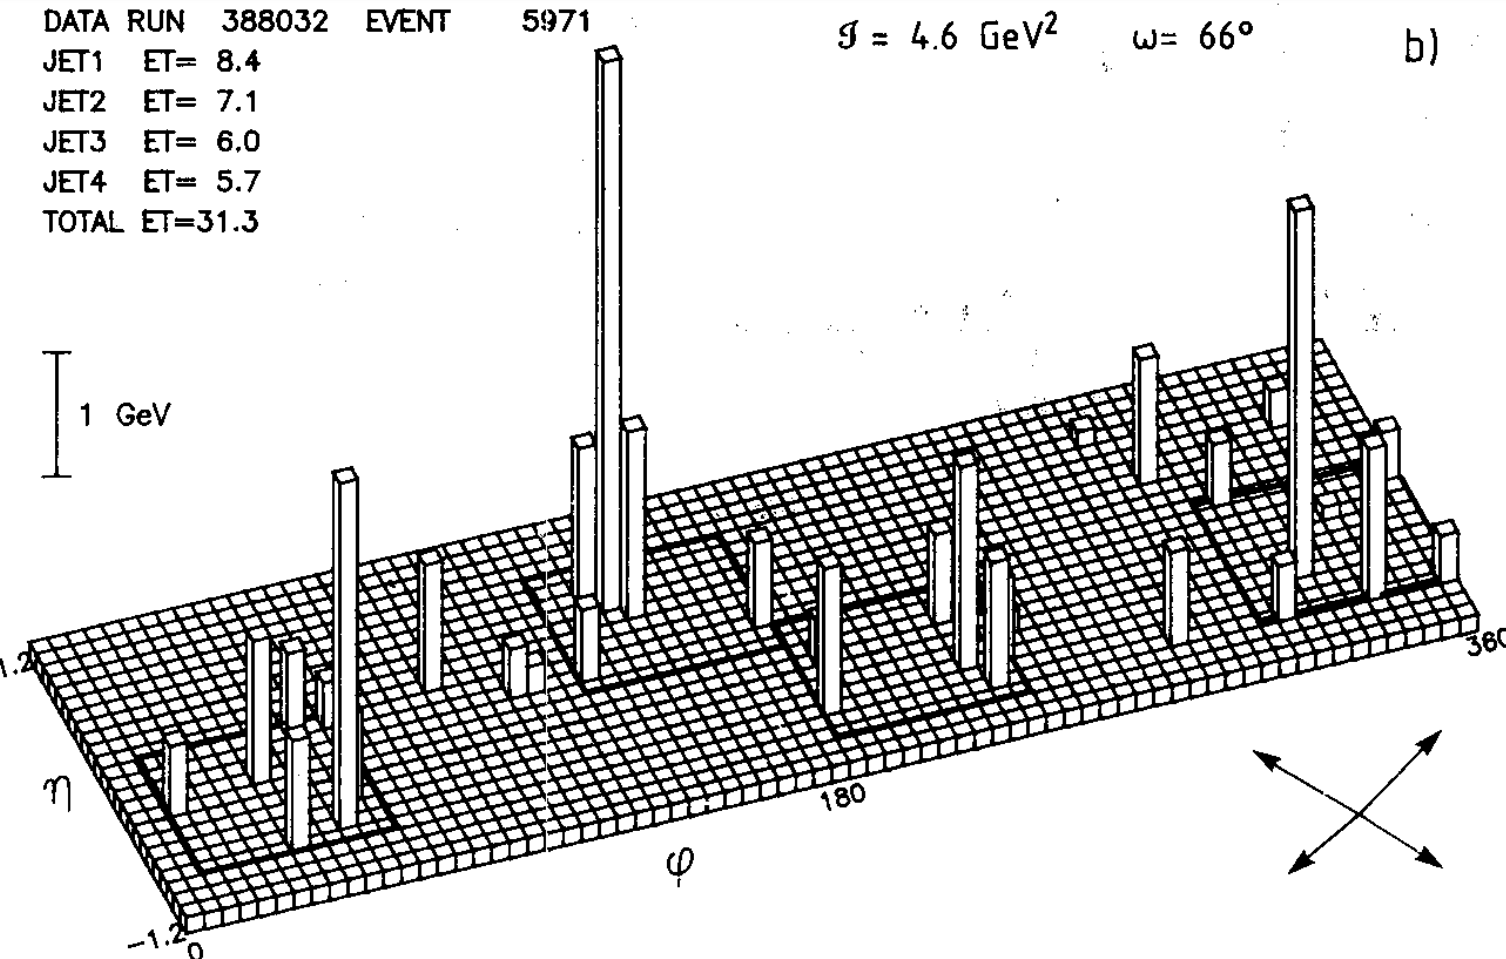
\includegraphics[width=.520\textwidth]{\imgpath/afs4jet.png}} 
\subfloat[][]{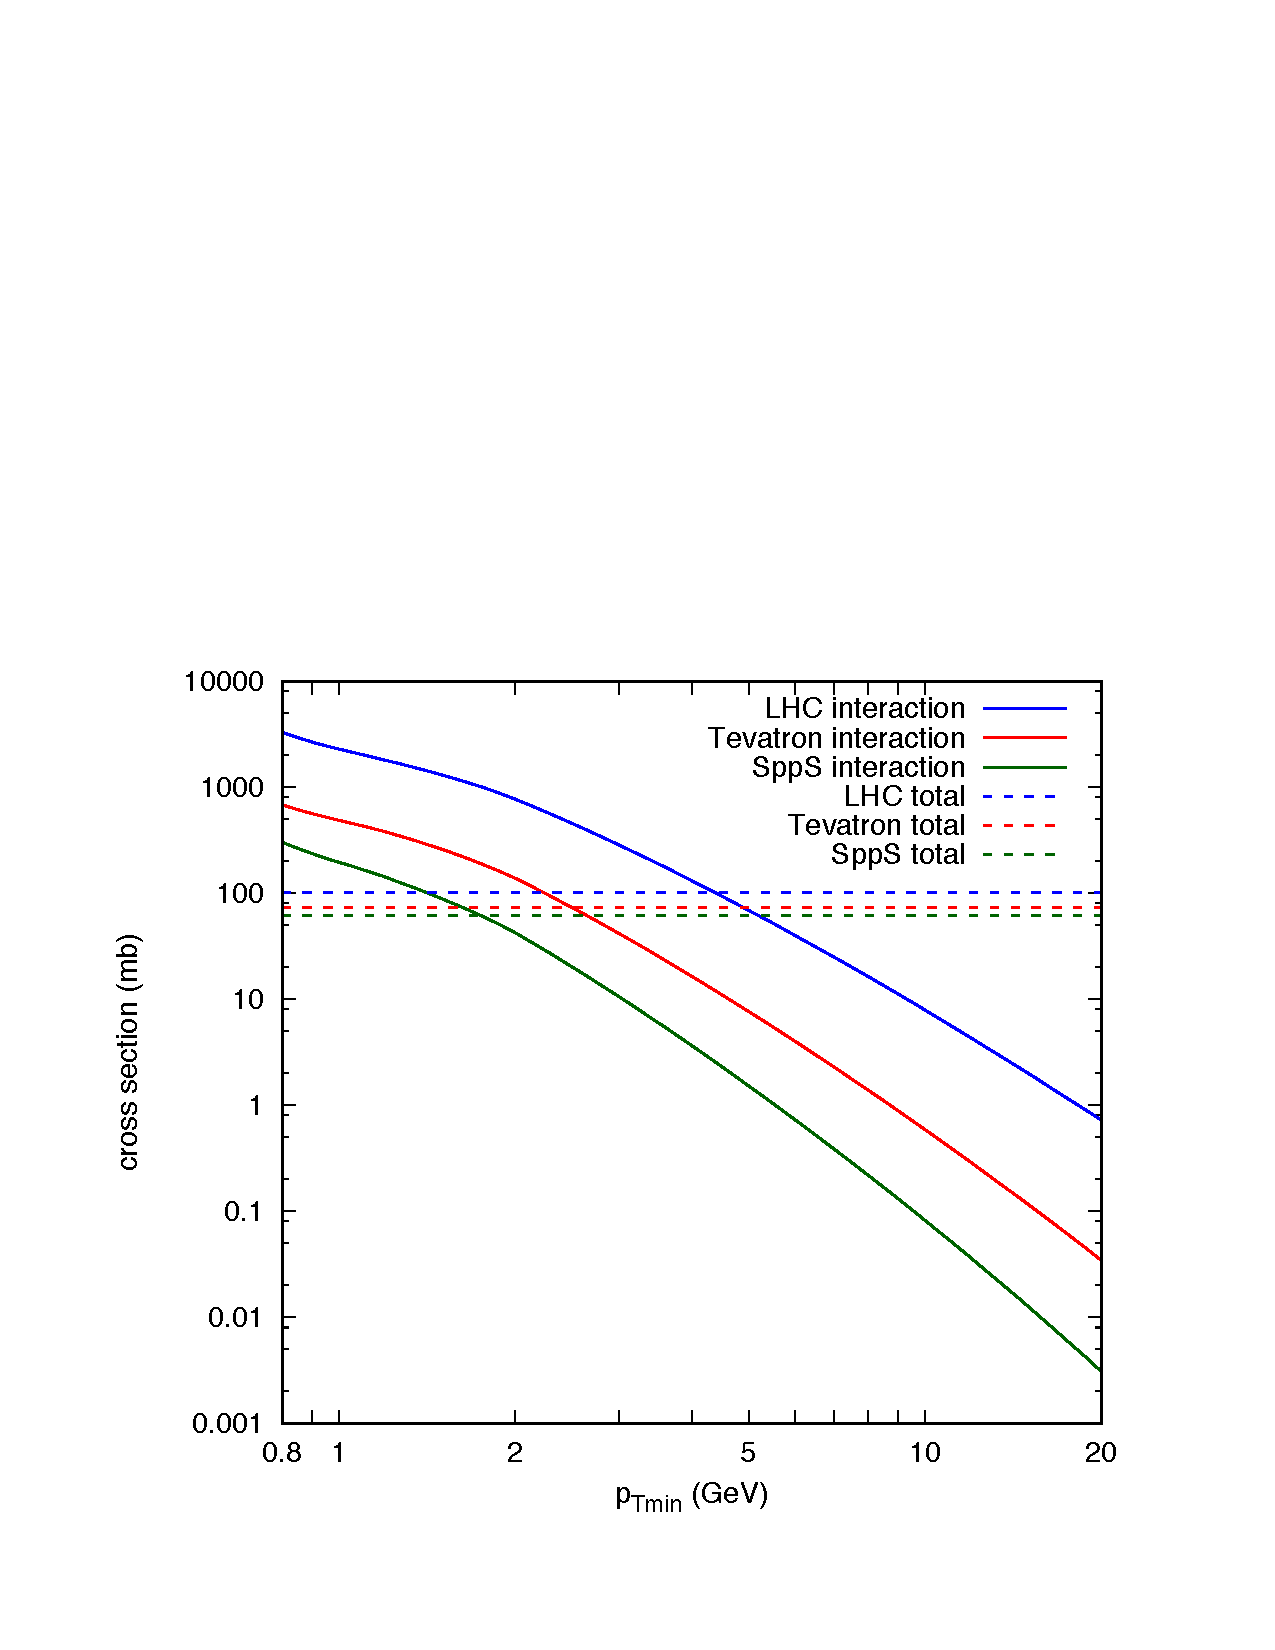
\includegraphics[width=.380\textwidth]{\imgpath/sigmampi.pdf}}
\caption{\textbf{(a)} Event display of an event with a 4-jet, where the pillars correspond to transverse energy deposits. \cite{akessonDoublePartonScattering1987} \textbf{(b)} Dependence of the integrated parton-parton cross section on the cutoff parameter $k_{\perp \mathrm{min}}$ for $\mathrm{Sp\bar{p}S}$ at \sppt{0.63}, Tevatron at \sppt{1.96}, and the LHC at \sppt{13}, modelled with Pythia. \cite{sjostrandDevelopmentMPIModelling2017}}
\label{fig:intro:afs4jet}
\end{figure}

These findings prompted further development of Regge theory and approaches that incorporated multiple pomerons, which were successful in describing the \Nch distributions. However, this approach is fully decoupled from descriptions of the perturbative primary scattering. Subsequently, much of the phenomenology related to multiple partonic interactions was developed within the framework of the Pythia MC event generator, which is discussed individually in Chapter~\ref{chap:colls} \cite{sjostrandDevelopmentMPIModelling2017}. However, nowadays, the relevance of the concept of MPIs in hadronic collisions extends beyond this generator. A scattering with double partonic interactions is illustrated in Fig.~\ref{fig:intro:dps}.

\begin{figure}[H]
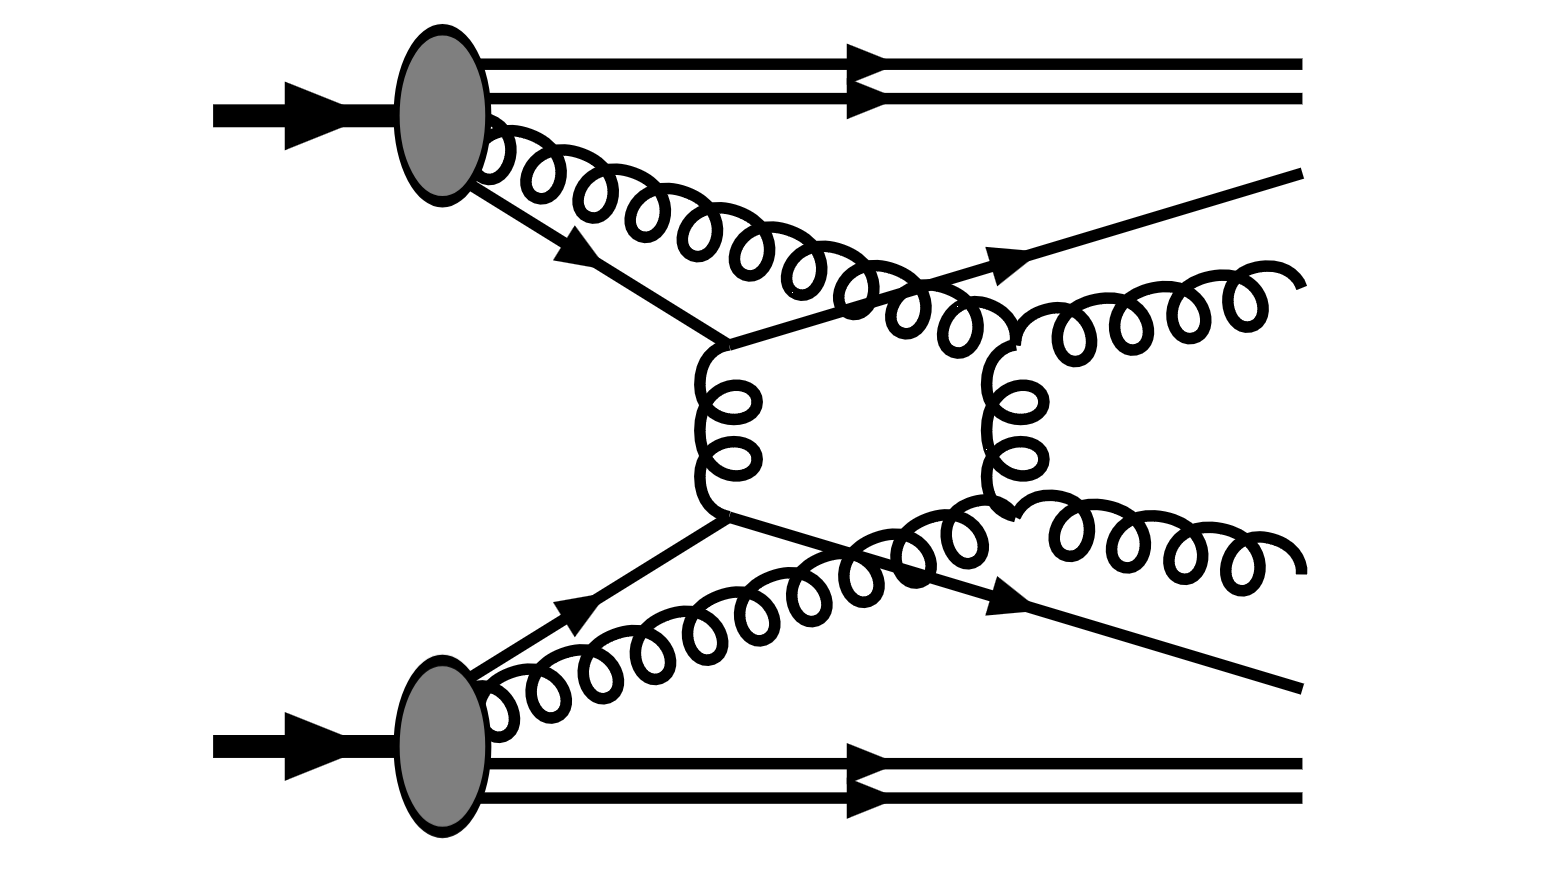
\includegraphics[height=7em]{\imgpath/dps.png}
\caption{Diagram showing a double partonic interaction, a case of $\nmpi=2$. \cite{prestelParticlePhysicsPhenomenology}}
\label{fig:intro:dps}
\end{figure}

In the Pythia approach, MPI are treated as additional perturbative scatterings. In QCD, the $2\to2$ cross section (dominated by the gluon exchange t-channel) diverges as $\propto \alpha^2_S(k_{\perp}^2)/k_{\perp}^4$, so a cutoff parameter $k_{\perp\mathrm{min}}$ must be introduced, and using (\ref{eq:intro:factorization}) leads to:
\begin{align}
\frac{d\sigma}{dk_{\perp}^2} &= \sum_{ij}\int dx_1 dx_2 f_i(x_1,\mu_F^2)f_j(x_2,\mu_F^2) \frac{d\hat{\sigma}^H_{ij}}{dk_{\perp}^2} \, , \\
\sigma_{\text{int}}(k_{\perp\text{min}}) &= \int_{k_{\perp\text{min}}^2}^{s/4} \frac{d\sigma}{dk_{\perp}^2}dk_{\perp}^2 \, .
\end{align}
The choice of cutoff can be tuned to experimental data, and for the $\mathrm{Sp\bar{p}S}$ energy of \sppg{630}, a value of around \gevc{1.6} was typical \cite{sjostrandDevelopmentMPIModelling2017}. The dependence of this parton-parton scattering cross section is shown in Fig.~\ref{fig:intro:afs4jet}.

The total pp cross-section, which is on the order of $100$~mb at \sppt{13}, is given by
\begin{align}
\sigma_{\mathrm{pp}} &= \sigma_{\mathrm{elastic}} + \sigma_{\mathrm{single \, dif.}} + \sigma_{\mathrm{double \, dif.}} + \sigma_{\mathrm{non-dif.}} \quad , 
\end{align}
where the inelastic cross sections $\sigma_\mathrm{inel} \approx \sigma_{\mathrm{double \, dif.}} + \sigma_{\mathrm{non-dif.}}$ corresponds to approximately 60\% of the total. The mean number of MPIs, \meannmpi, can be estimated using:
\begin{align}
\meannmpi (k_{\perp,\mathrm{min}}) = \frac{\sigma_{\mathrm{int}}(k_{\perp,\mathrm{min}})}{\sigma_{\mathrm{inel}}}
\end{align}

However, the actual treatment is more complex and involves considerations of other parameters such as the dampening factor $k_\perp^0$ to account for the confinement nature of partons, modifications of multiparton PDFs, energy-momentum conservation effects, $x$-dependent source geometry, and the intertwinedness of partonic evolutions.


In summary, MPIs represent several subcollisions that take place in an average pp collision with \pt scales of a few GeV. They are colour-connected to the beam remnants, which in the Lund model are represented by strings. Since a string with $\kappa = 1 \mathrm{GeV} /\mathrm{fm}$ yields, as a rule of thumb, approximately one hadron per unit rapidity, and the average pp collision at the LHC at \sppt{13} has $\langle \dndy \rangle \approx 6$, the typical number of partonic interactions is around six \cite{sjostrandDevelopmentMPIModelling2017}.

Finally, the observation of QGP-like phenomena in pp collisions at the LHC has renewed interest in MPI phenomenology, as discussed in the following chapter. Such observations do not contradict the concept of MPIs; rather, they suggest the possibility of incorporating collective behavior among the MPIs, such as interactions between strings, local modifications of string tensions, or, alternatively, the formation of a multipartonic state with QGP-like properties.

\subsection{Colour reconnection}

The incorporation of MPIs improved the description of the \Nch distributions and their dependence on $\sqrt{n}$. However, there were also observations of $\meanpt(\Nch)$ increasing as a function of \Nch, which could not be explained. More MPIs lead to more strings, which in turn leads to the production of more particles, but the \pt is mostly unaffected. This would predict a weaker dependence of \meanpt on \Nch, contrary to the data \cite{sjostrandDevelopmentMPIModelling2017}. The issue was resolved by implementing a possible color reconnection mechanism, which rearranges the color fields between partons.

\textit{TBA Insert diagrams of the processes!}

One can envision the following process:
\begin{align*}
e^+ e^- \rightarrow W^+ W^- \rightarrow q_1\bar{q}_2 q_3\bar{q}_4  .
\end{align*}
In this scenario, a color reconnection mechanism could rearrange the colour-connected $q_1\bar{q}_2$ and $q_3\bar{q}_4$ into $q_1\bar{q}_4$ and $q_3\bar{q}_2$ if it were energetically favourable, depending on the phase-space configurations. Measurements at LEP \cite{ElectroweakMeasurementsElectron2013} of this process have indeed shown that such final-state corrections must be taken into account to explain the data on $W$ masses and widths. They also reported that the reconnection probabilities for such events are on the order of $50\%$, further indicating that colour reconnection is an important factor to consider.

Pythia implements CR by minimizing the total length of strings in the system, analogous to minimising potential energy \cite{bierlichComprehensiveGuidePhysics2022}. This mechanism, illustrated in Fig.~\ref{fig:intro:cr}, explains the rising trend of $\meanpt$ as a function of \Nch: shorter strings imply fewer hadrons to split the transverse boost across, and the more MPI, the bigger this effect. Moreover, CR also helped describe the absolute value of \meanpt. With this approach, no further modifications of fragmentation parameters were necessary, in line with the concept of jet universality. However, it should be noted that there are various CR implementations and all rely on parameters obtained from tuning to data.

\begin{figure}[H]
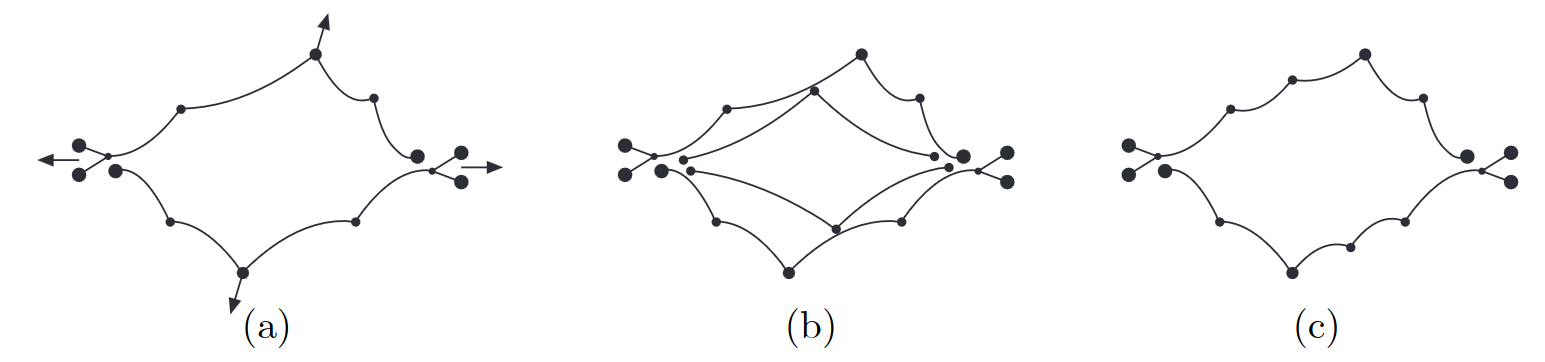
\includegraphics[height=7em]{\imgpath/cr.png}
\caption{Depiction of the CR process: \textbf{(a)} in a hard parton subcollision, the outgoing gluons are connected to the beam remnants through colour. Additional gluon kinks may occur through initial state radiation, which are ordered by rapidity. \textbf{(b)} A second hard scattering should theoretically result in two new strings connected to the remnants. \textbf{(c)} In order to minimise the total string length, gluons are colour reconnected. \cite{gustafsonMultipleInteractionsSaturation2009}}
\label{fig:intro:cr}
\end{figure}

It is also worth noting that the \pt boost acquired through color reconnection may depend on mass and whether a hadron is a baryon or meson, which somewhat mimics the hydrodynamic signatures of collective flow observed in AA collisions \cite{ortizColorReconnectionFlowlike2013}.

\section{Underlying event}\label{sec:intro:ue}

The underlying event (UE) in high-energy collisions refers to the additional hadronic activity that accompanies the primary hard scattering process, but is not directly related to it. This includes the fragmentation products of the beam remnants, ISR and FSR, as well as the effects of the previously discussed MPIs, and is visualised in Fig.~\ref{fig:intro:ue}. The UE (with its name coined at Tevatron \cite{cdfcollaborationChargedJetEvolution2002}) is typically characterized by a distribution of softer particles around and far outside of the hard process and was first observed at $\mathrm{Sp\bar{p}S}$ in the 1980s \cite{arnisonHadronicJetProduction1983}. These measurements saw a constant plateau of transverse energy $E_\mathrm{T}$ outside of the jet core, with its height independent of the jet energy.

\begin{figure}[H]
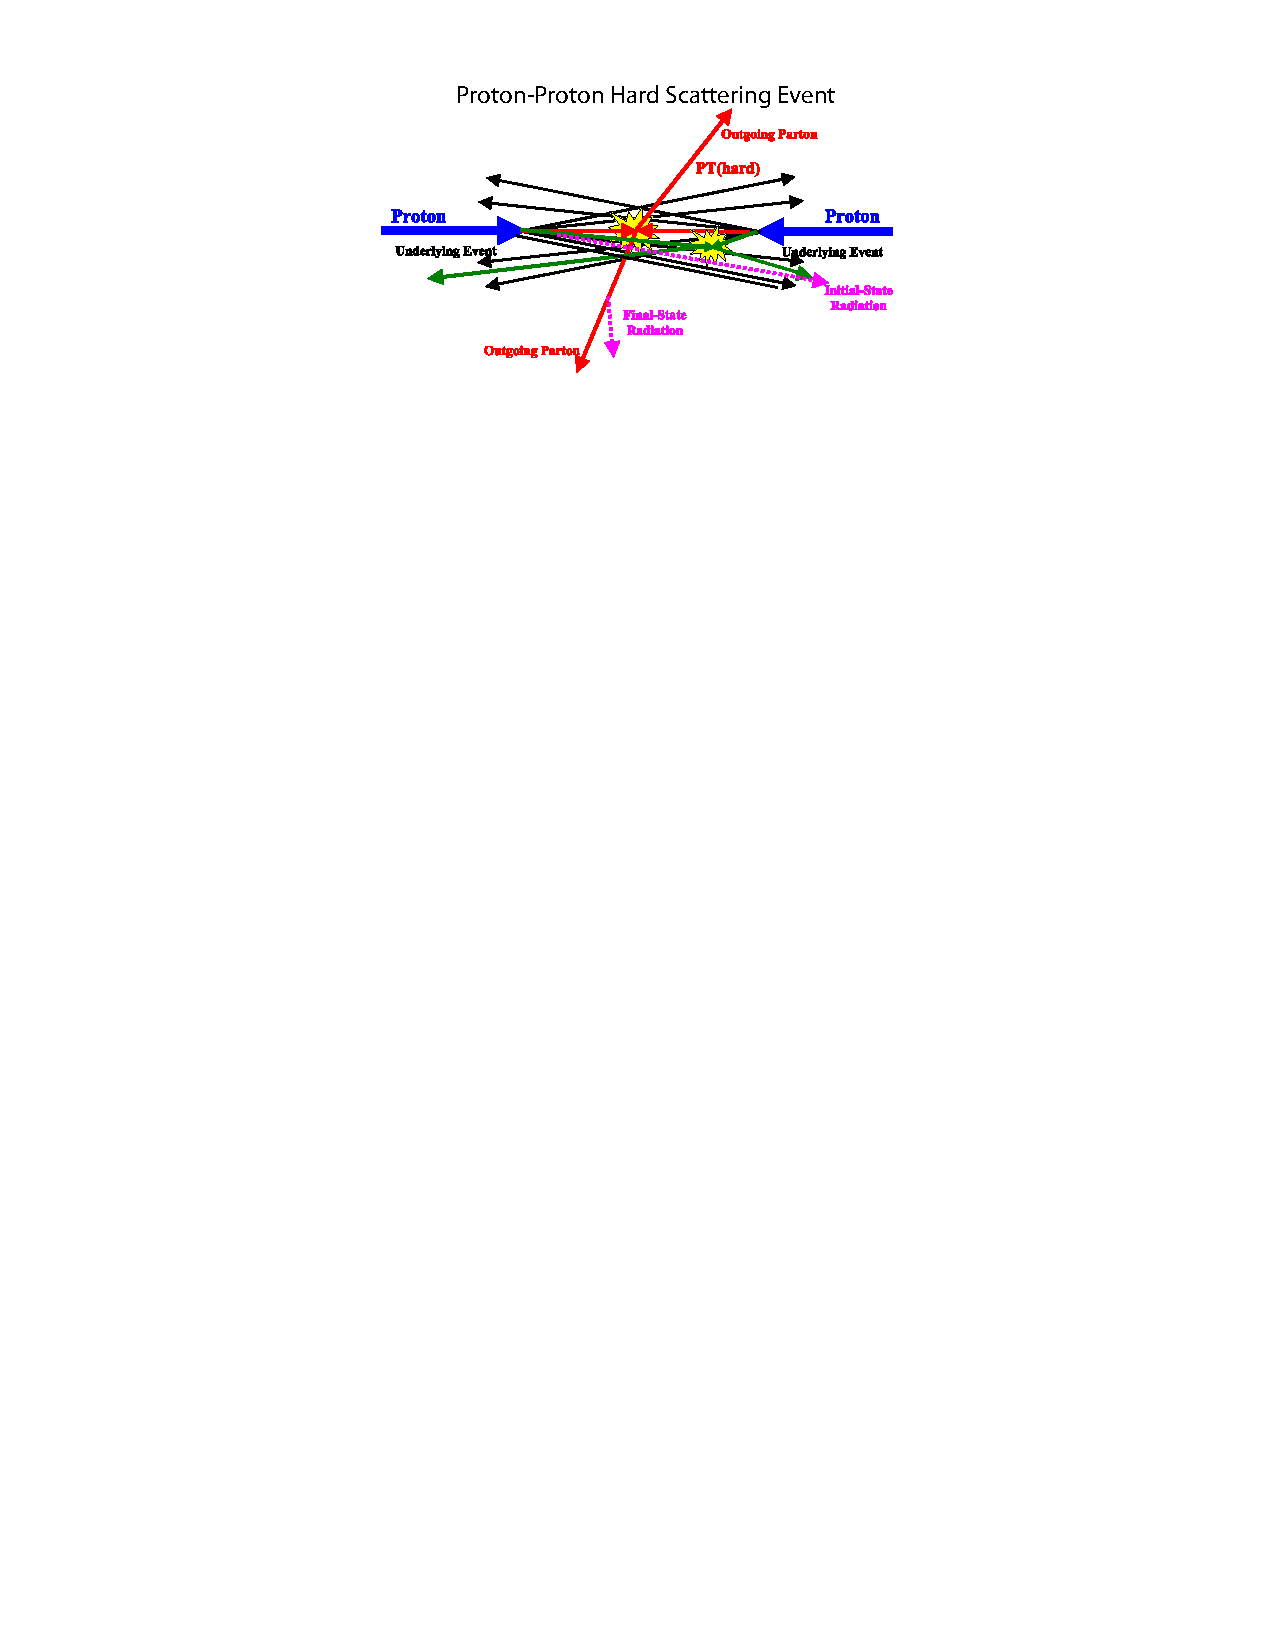
\includegraphics[width=.7\textwidth]{\imgpath/ue.pdf}
\caption{Cartoon illustrating a pp collision and its components: the hard scattering process, beam remnants, initial/final state radiation, and the MPIs. The last three contribute to the underlying event. \cite{cainesUnderlyingEventStudies2009, cdfcollaborationChargedJetEvolution2002}}
\label{fig:intro:ue}
\end{figure}

It is important to note that particle production in UE is different from the MB production, as it is biased by the presence of hard scattering. Additionally, the magnitude of the UE can fluctuate significantly from event to event.

\section{From hadrons to partons: deconfined QCD matter}

A simple argument can be made that confinement of quarks inside hadrons cannot be sustained when the density of partons is too large compared to that inside ordinary hadrons. Or alternatively, when the partonic kinetic energies are much larger than the confining part of the $q\bar{q}$ potential in (\ref{eq:intro:qqpot}). The following sections introduce some theoretical frameworks predicting the deconfinement of quarks and gluons. The calculations presented use natural units ($\hbar = c = k_B = 1$).

\subsection{Bag model of hadrons}

In this very naive approach \cite{detarBAGMODELSHADRONS1983, matonohaUpsilonMesonProduction2018}, hadrons are treated as spherical cavities (``bags") with radius $R$ of free massless quarks. These cavities exist in the non-perturbative QCD vacuum, which exerts a confining pressure $B$. The lowest-energy solution of the Dirac equation for the quarks, which in this case is $\slashed p \psi = 0$, is the $s_{1/2}$-state given by:
\begin{align}
\psi (r, t) = N \begin{pmatrix} j_0(\omega r) U \\ i \sigma \cdot \hat{r} j_1(\omega r) U \end{pmatrix} \exp (-i \omega t) \quad ,
\end{align}
where $N$ is a normalisation constant, $j_0$ and $j_1$ are spherical Bessel functions, $\omega$ is the quark energy, and $U$ the two-component spinor. The assumption that quarks are confined within the cavity volume represents the boundary conditions that the quark scalar density $\psi \bar{\psi}$ becomes zero at $r=R$, which is equivalent to $j_0(\omega R) = j_1(\omega R)$:
\begin{align}
j_0^2(\omega R) - \vec{\sigma} \cdot \hat{r} \vec{\sigma} \cdot \hat{r} j_1^2(\omega R) = 0 \\
j_0(\omega R) = j_1(\omega R) \quad ,
\end{align}
which happens when $\omega \approx \frac{2.04}{R}$. Thus, energy of the system can be given by
\begin{align}
E(R) \approx n_q \cdot \frac{2.04}{R} + \frac{4\pi}{3} B R^3 \quad .
\end{align}
Here, the first term represents the kinetic energy of $n_q$ quarks in the cavity and second term is the cavity volume energy. Gluon solutions should also be considered but are neglected in this approach. The first term acts to expand the cavity, whereas the second term acts to contract it. Finding an optimum of this energy with respect to $R$ leads to
\begin{align}\label{eq:intro:bagp}
B^{1/4} \approx \left( \frac{2.04 n_q}{4\pi} \right)^{1/4} \frac{1}{R} \quad .
\end{align}
Finally, assuming values for a proton, $R\approx 0.8$~fm, and three valence quarks $n_q=3$, the confining pressure can be approximated as $B^{1/4} \approx 206$~MeV. \cite{detarBAGMODELSHADRONS1983}

To relate the confining pressure to a critical temperature at which deconfinement occurs, $T_c$, one can assume a gas of relativistic massless fermions and bosons with energy density $\rho$ \cite{wongIntroductionHighEnergyHeavyIon1994, mcgreevyLectureNotesQuantum}. Using Stefan-Boltzmann law, the equation of state is,
\begin{equation}
P = \frac{1}{3} ( d_b + \frac{7}{8} d_f ) \rho = ( d_b + \frac{7}{8} d_f ) \frac{\pi^2}{90} T^4 \,
\end{equation}
where $d_b$ and $d_f$ are the degeneracy numbers for bosons and fermions, in this case gluons and quarks, respectively. Summing together possible colours, polarisations, and flavours for particles and antiparticles, one gets $d_b = 16$ and $d_f = 24$. Inserting the cavity pressure $B$ value calculated in (\ref{eq:intro:bagp}), $T_c$ can be estimated as approximately $145$~MeV.

\subsection{Lattice QCD}

Lattice QCD (LQCD) is a technique allowing calculation of processes involving the strong interaction in the non-perturbative regime, from first principles, without phenomenological assumptions. In this approach, the space-time continuum is discretised into a four-dimensional lattice, which allows QCD path integrals to be solved numerically. Smallest squares on the lattice are called \textit{plaquettes}, with the lattice links representing gluon fields and lattice sites representing quark fields. \cite{meyerLatticeQCDBrief2015}

Lattice calculations are computationally extremely intensive\footnote{In fact, in the past, LQCD was among important drivers of the advancement of GPU computing and it is also used as benchmark in high-performance computing \cite{bennettBSMBenchFlexibleScalable2016}.}, thus, a sufficiently coarse lattice spacing must be chosen to reduce computational costs and make the approach feasible. Often, simulations are also performed with unphysical quark masses (e.g.\ $m_q \sim m_\pi$), for the same reason. The results are then extrapolated using highly complex methods. Another limitation in LQCD is the so-called \textit{sign problem}, discussed in detail for instance in Ref.~\cite{nagataFinitedensityLatticeQCD2022}, which arises when evaluating highly oscillatory complex integrals in finite-density environment.

Despite its challenges, LQCD has been successful in various predictions, notably, the \textit{ab initio} calculation of the mass of neutron (uud) using the mass of $\Omega$ (sss) as an input \cite{durrInitioDeterminationLight2008}. Furthermore, it allows for the calculation of thermodynamics of QCD matter and predicts its equation of state, as well as a phase transition at $T_c \approx 150$~MeV \cite{petreczkyLatticeQCDNonzero2012, bazavovEquationStateFlavor2014}, which is usually identified with the formation of quark-gluon plasma QGP, discussed in Chapter~\ref{chap:colls}. The dependence of energy density and pressure on temperature can be seen in Fig.~\ref{fig:intro:eos}.

\begin{figure}[H]
\subfloat[][]{\adjustbox{valign=m}{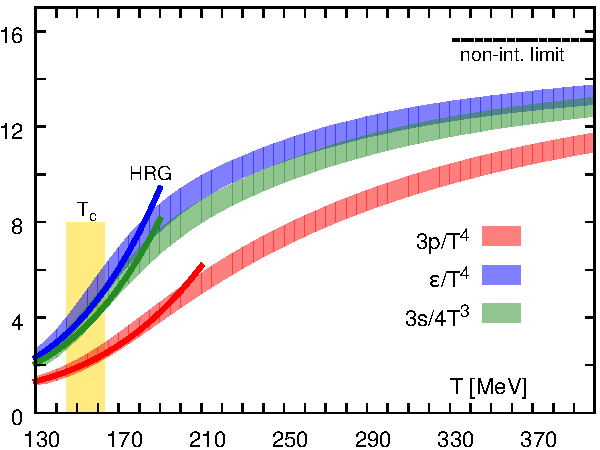
\includegraphics[width=.40\textwidth]{\imgpath/eos.pdf}}}\hspace{1.5em}%
\subfloat[][]{\adjustbox{valign=m}{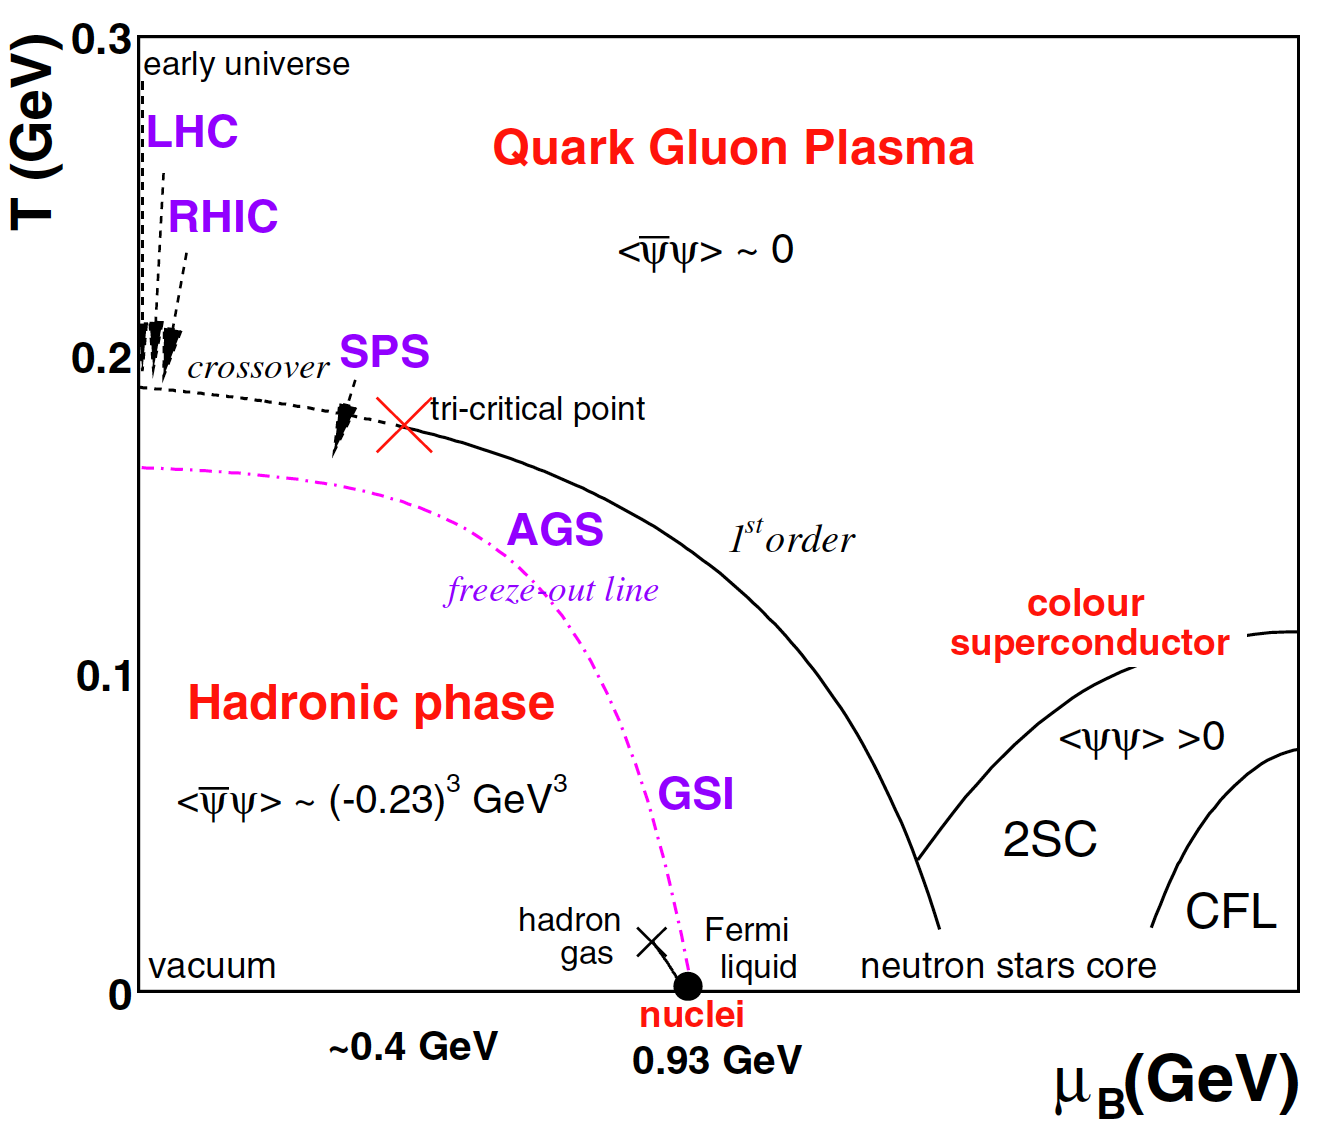
\includegraphics[width=.50\textwidth]{\imgpath/phasediagram.png}}}
\caption{\textbf{(a)} Dependence of the pressure (red), energy density (blue), and entropy density (green) on temperature, determined with LQCD. \cite{bazavovEquationStateFlavor2014} \textbf{(b)} Phase diagram of QCD matter. \cite{pasechnikPhenomenologicalReviewQuark2017}}
\label{fig:intro:eos}
\end{figure}

\subsection{QCD phase diagram, chiral symmetry restoration}

Phase transitions of QCD matter are investigated to explore the QCD phase diagram with respect to temperature $T$ and baryon chemical potential $\mu_B$, which corresponds to net baryon density. Figure~\ref{fig:intro:eos} visualizes the different areas of the QCD phase diagram probed by various experiments \cite{pasechnikPhenomenologicalReviewQuark2017}. Measurements of Pb-Pb collisions at the LHC access high $T$ and almost zero $\mu_B$, as the nucleons of ultrarelativistic Pb nuclei escape the interaction volume before the plasma develops, and the high energy subsequently leads to a sizable baryon production balanced by anti-baryons due to conservation laws. Experiments studying collisions of slower and heavier nuclei reach higher $\mu_B$ regions.

Furthermore, looking back at the QCD Lagrangian in (\ref{eq:intro:lqcd}) and neglecting quark current masses $m_{u,d}\to 0$, it can be seen that it is invariant when switching the up and the down quark, corresponding to a SU($2$) isospin symmetry. This allows the fermion fields to be rewritten in terms of their left and right chiralities and the QCD Lagrangian then exhibits a larger \textit{chiral symmetry}.

However, it is known that the vacuum expectation value of a $q\bar{q}$ state is much larger than the current masses $m_{u,d}$:
\begin{equation}
\langle 0 | q \bar{q} | 0 \rangle = \langle 0 | u\bar{u} + d \bar{d} | 0 \rangle \approx (250 \, \mathrm{MeV} )^3 \quad ,
\end{equation}
where the value is taken from average masses of light flavour mesons. This means that the QCD vacuum spontaneously breaks the chiral symmetry. \cite{sazdjianIntroductionChiralSymmetry2017}

It can be expected that in the plasma of deconfined quarks and gluons, chiral symmetry is \textit{restored} \cite{gottliebEstimatingChiralsymmetryRestoration1987, xuChiralSymmetryRestoration2023}. This is actively studied in AA collisions, for example in searches of the so-called chiral magnetic effect \cite{starcollaborationSearchChiralMagnetic2021} or degeneracy of normally chiral partners \cite{hohlerRmesonMeltingCompatible2014}, such as the $\rho$ ($J^P=1^-$) and $a_1$ ($J^P=1^+$) states.

%\section{Implications of high-activity QCD research}
%
%Understanding the early universe: The QGP is believed to have existed in the first few microseconds after the Big Bang. Studying QGP can provide insight into the behavior of matter and the formation of the universe
%Understanding of fundamental physics: QGP is a unique state of matter that is not well understood. Studying QGP can provide insight into the behavior of quarks and gluons, which are the building blocks of matter.
%Developing a deeper understanding of strong interactions: The strong nuclear force is one of the four fundamental forces of nature. Studying QGP can provide insight into the behavior of this force and its interactions with matter.
\chapter{QCD phenomena in high energy hadronic collisions}
\def \imgpath {"./figures/colls"}

The aim of this chapter is to give an introduction to the physics of heavy ions and the various phenomena related with the quark-gluon plasma QGP. Furthermore, a detailed summary of the findings of QGP phenomena in small systems, i.e.\ pp and pA collisions, is given. Lastly, some Monte Carlo event generators based on phenomenological modelling of hadronic collisions relevant to this dissertation are summarised.

\section{Collisions of heavy nuclei}

\subsection{Collision geometry, centrality, multiplicity}

Collisions of heavy nuclei, composed of many fluctuating nucleons, may occur under various initial state configurations. Some quantities used to describe them are the impact parameter $b$, defined as the distance between the two nuclei centers, number of participating (scattered) nucleons $\Npart$, and the number of binary nucleonic collisions $\Ncoll$.

Determining these quantities is important because:
\begin{enumerate}
\item Soft processes, such as light flavor particle production, are expected to scale with the interaction volume, which $\propto \Npart$.
\item Hard processes, such as jet and heavy flavor production, are expected to scale with the number of large momentum transfer interactions given by \Ncoll.
\item $b$, disregarding the fluctuations of nucleonic positions, defines the shape and anisotropy of the overlap region, which are important initial state conditions.
\end{enumerate}

Since these quantities cannot be directly measured, they need to be modelled. The charged particle \textit{multiplicity} is commonly used for this purpose, as \meanNch increases monotonically with \Npart, \Ncoll, and decreasing $b$. Multiplicity \Nch can be measured experimentally, e.g.\ with tracking detectors. The concept of \textit{centrality} is also used, which is defined as quantiles of the total nuclear cross-section. For example, a centrality of $0-5\%$ refers to low $b$ values and the top $5\%$ of \Nch values (central events), while $95-100\%$ centrality refers to high $b$ values and the bottom $5\%$ of \Nch values (peripheral events). Centrality can also be inferred from other \textit{event activity} classifiers, such as amplitudes of scintillators at forward rapidity, transverse energy in calorimeters, or energy from beam remnants in zero-degree-calorimeters.

In AA collisions, these relationships are well-defined, and thus the models perform well. The most popular model is the MC Glauber model \cite{millerGlauberModelingHigh2007}. Other models include MC-KLN \cite{kharzeevHadronProductionNuclear2001} and IP Glasma \cite{schenkeFluctuatingGlasmaInitial2012}.

\subsection{MC Glauber model}

The MC Glauber model \cite{millerGlauberModelingHigh2007} takes on a very simple albeit powerful approach. The two nuclei are simulated in three dimensions in a way that satisfies their respective nuclear density profiles, usually modelled by sampling the positions of nucleons from the Woods-Saxon distribution:

\begin{minipage}{0.4\linewidth}
    \begin{center}
        \begin{tikzpicture}
            \draw[->] (-0.25,0) -- (2.5,0) node[right] {$r$};
            \draw[->] (0,-0.2) -- (0,1.2) node[above] {$n(r)$};
            \draw[scale=1,domain=-0.15:2.2,smooth,variable=\x,blue] plot ({\x},{1/(1+exp((\x-1.5)/0.1))});
            \draw[dashed] (1.5,0) node[below] {$R$} -- (1.5,1);
        \end{tikzpicture}
    \end{center}
\end{minipage}%
\begin{minipage}{0.6\linewidth}
    \begin{equation}
        n(r) = \frac{1}{1+\exp((r-R)/a)} \quad ,
    \end{equation}
\end{minipage}

where $R$ is the nuclear radius and $a$ the nuclear skin thickness.

The nucleonic densities can be represented by uniform disks, or more accurately by Fermi-distributions or Gaussian profiles to account for fluctuations of their densities. Their parameters are left free and are tuned to the data.

A random impact parameter is then chosen or sampled. The collision is then treated as a sequence of independent binary nucleon-nucleon collisions, where
\begin{enumerate}
\item nucleons remain travelling in straight lines,
\item the inelastic nucleon-nucleon cross section $\sigma_\mathrm{NN}$ does not depend on the number of interactions,
\item two nucleons are considered to interact if their transverse relative distance $d \leq \sqrt{\sigma_\mathrm{NN}/\pi}$.
\end{enumerate}

Figure~\ref{fig:colls:centrality} illustrates an example of a Glauber Monte Carlo event for a Au+Au collision. By simulating numerous collisions, the average \Npart and \Ncoll are determined\footnote{It also shows the scaling between the numbers of participants and binary collisions, which is approximately $\Ncoll \approx 0.35 \Npart^{4/3}$ .}, and their relations to centrality and event activity observables are determined by fitting to experimental data.

Recent studies have extended the MC Glauber model to include sub-nucleonic structures. Such efforts show that the production of charged hadrons at mid-rapidity scales linearly with the number of participating partons. Comparisons with LHC data at \snnt{5.02} suggest that the number of sub-nucleonic degrees of freedom ranges from $3$ to $5$ \cite{loizidesGlauberModelingHighenergy2016}.

\begin{figure}[H]
\subfloat[][]{\adjustbox{valign=m}{\adjincludegraphics[trim={{.33\width} 0 {.33\width} 0},clip,width=.29\textwidth]{\imgpath/glauber_mc_event.pdf}}}\hspace{2em}
\subfloat[][]{\adjustbox{valign=m}{\includegraphics[width=.490\textwidth]{\imgpath/cocktail3.eps}}}
\caption{\textbf{(a)} Glauber Monte Carlo event of a Au+Au collision at \snng{200} shown in the transverse plane (top panel) and along the beam axis $z$ (bottom panel). The darker circles represent participating nuclei and their area corresponds to $\sigma_\mathrm{NN}$. \textbf{(b)} Illustrative diagram of the dependence of final-state event multiplicity on the initial-state quantities, number of participants \Npart and impact parameter $b$. \cite{millerGlauberModelingHigh2007}}
\label{fig:colls:centrality}
\end{figure}

\section{Quark-gluon plasma}

In agreement with lattice QCD predictions \cite{borsanyiThermodynamicsQCDTransition2013}, the QGP has been measured in ultra-relativistic collisions of heavy nuclei at RHIC \cite{arseneQuarkGluonPlasma2005, adamsExperimentalTheoreticalChallenges2005}, LHC \cite{niidaSignaturesQGPRHIC2021}, and even SPS \cite{heinzEvidenceNewState2000}. Although it cannot be observed directly, a wealth of evidence from three decades of research combining various observables reveals the effects of the produced QGP medium. Whilst somewhat context-dependent, the following features make QGP the most extreme phenomenon observed in terms of its:
\begin{itemize}
\item \textit{Temperature}: QGP temperatures reach values on the order of hundreds of MeV, which corresponds to approximately $2 \times 10^{12}$~K.\footnote{Contrasting some of the lowest temperatures required for the super-conducting magnets of the LHC, $T \approx 1.9$~K.} \cite{cmscollaborationMeasurementNuclearModification2019}
\item \textit{Viscosity}: the shear viscosity to entropy density ratio $\eta/s$ reaches the minimum quantum limit of $1/4\pi$ (for water at room temperature, $\eta/s \approx 8$), making it an almost perfect liquid. \cite{pasechnikPhenomenologicalReviewQuark2017}
\item \textit{Vorticity}: in semi-peripheral collisions, the rotating plasma reaches a vorticity of approximately $9\times 10^{21}$ s$^{-1}$. \cite{adamczykGlobalHyperonPolarization2017}
\item \textit{Magnetic field}: in non-central collisions, the magnetic fields in the system may peak at $\sim 10^{19}$ T. \cite{kharzeevEffectsTopologicalCharge2008}
\end{itemize}

\begin{figure}[H]
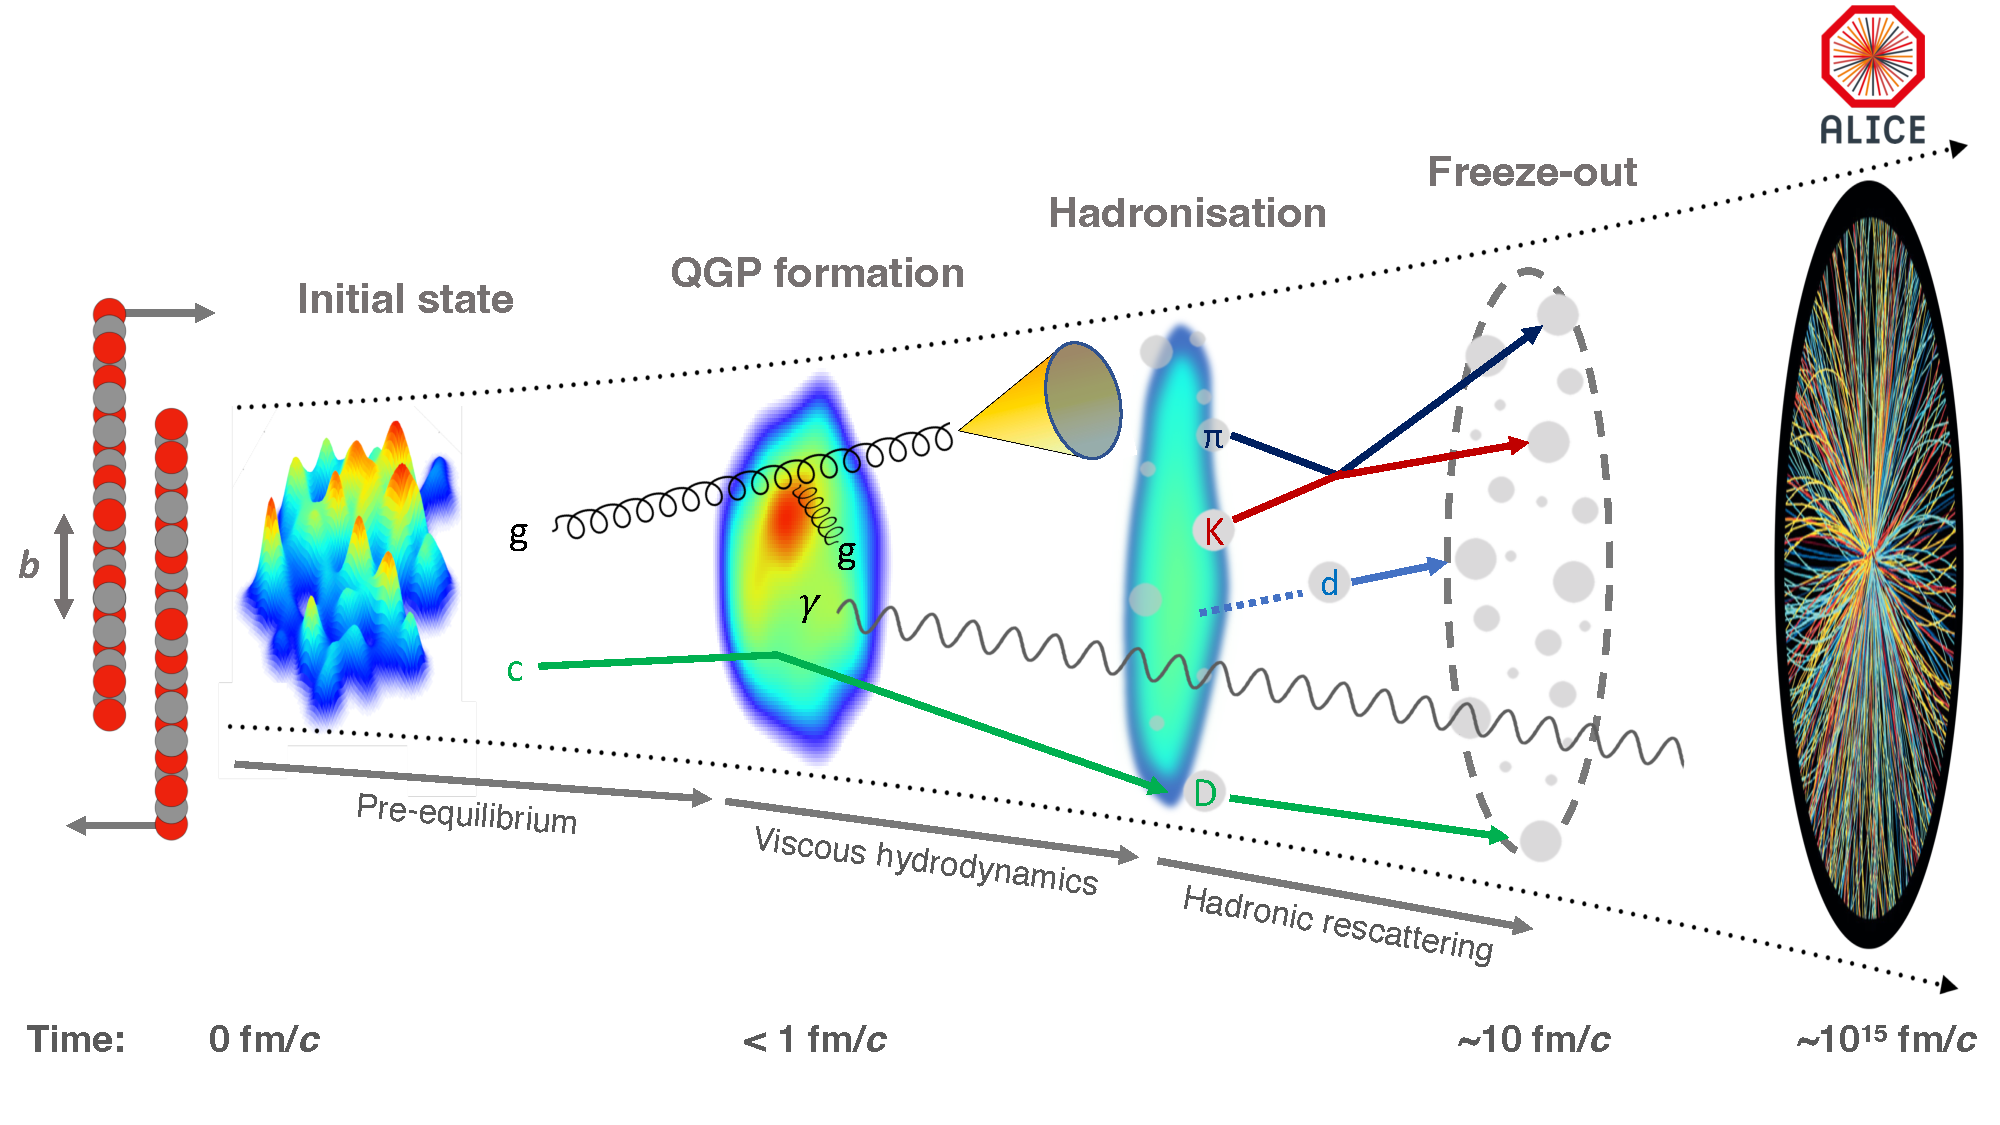
\includegraphics[width=.90\textwidth]{\imgpath/evolution.pdf}\\
\caption{Evolution of heavy nuclei collisions at LHC energies, depicting the different stages. \cite{alicecollaborationALICEExperimentJourney2022}}
\label{fig:colls:evolution}
\end{figure}

Figure~\ref{fig:colls:evolution} illustrates the common paradigm for the different stages of a collision between heavy nuclei:
\begin{enumerate}
\item The Lorentz-contracted heavy nuclei approach each other at ultra-relativistic speeds.
\item \textit{Pre-hydrodynamisation stage} ($\tau \equiv \sqrt{t^2 - z^2} \leq 1$ fm/c): ``hard" particles are produced in scatterings with the highest momentum transfer $Q^2$. Produced matter expands rapidly in the longitudinal direction and starts expanding in the radial direction.
\item \textit{Hydrodynamisation} ($1 \leq \tau \leq 10$ fm/c): abundantly produced partons create a deconfined medium, which can be described by hydrodynamic equations.
\item \textit{Chemical freeze-out} ($\tau \sim 10$ fm/c): the system cools down and hadronises. The produced hadrons then stop interacting inelastically and the system's chemical content is stabilised.
\item \textit{Kinetic freeze-out} ($\tau \lesssim 20$ fm/c): hadrons no longer interact elastically and their kinematics stabilize.
\item Long-lived particles can be measured in the detector volume. 
\end{enumerate}

The following subsections outline some of the essential phenomena related to the production of QGP.

\subsection{Quarkonium dissociation and sequential suppression}

Heavy quarkonia are vector meson states consisting of $c\bar{c}$ and $b\bar{b}$. They include $J/\psi$, $\psi(2\mathrm{S})$, $\Upsilon(1\mathrm{S})$, $\Upsilon(2\mathrm{S})$, $\Upsilon(3\mathrm{S})$, which can be relatively easily measured in LHC experiments via their di-lepton decay channels. They are created solely in the first phases of the collision and then experience the entire evolution of the QGP medium:
\begin{equation}
t^{Q\overline{Q}}_\mathrm{creation} < t^\mathrm{QGP}_\mathrm{creation} < t^\mathrm{QGP}_\mathrm{lifetime} \ll t^{Q\overline{Q}}_\mathrm{lifetime} \quad .
\end{equation}

Additionally, due to their large binding energies, their radii may remain smaller than the plasma screening radius $r_\mathrm{D}(T)$, and thus, survive the dissociation. For instance, considering their in-vacuum radii determined from the $q\bar{q}$ potential, $r_{\Upsilon(1\mathrm{S})}\sim 0.14$~fm, $r_{\Upsilon(2\mathrm{S})}\sim 0.28$~fm, $r_{\Upsilon(3\mathrm{S})}\sim 0.39$~fm, which contrast the $r_\pi \sim 0.7$~fm \cite{sarkarPhysicsQuarkGluonPlasma2010}. This implies that different temperatures result in the dissociation of different states, and measuring the production of different states can help infer the QGP temperature, as illustrated in Fig.~\ref{fig:colls:thermometer} \cite{matsuiSuppressionQuarkgluonPlasma1986, satzProbingStatesMatter2013}.

\begin{figure}[H]
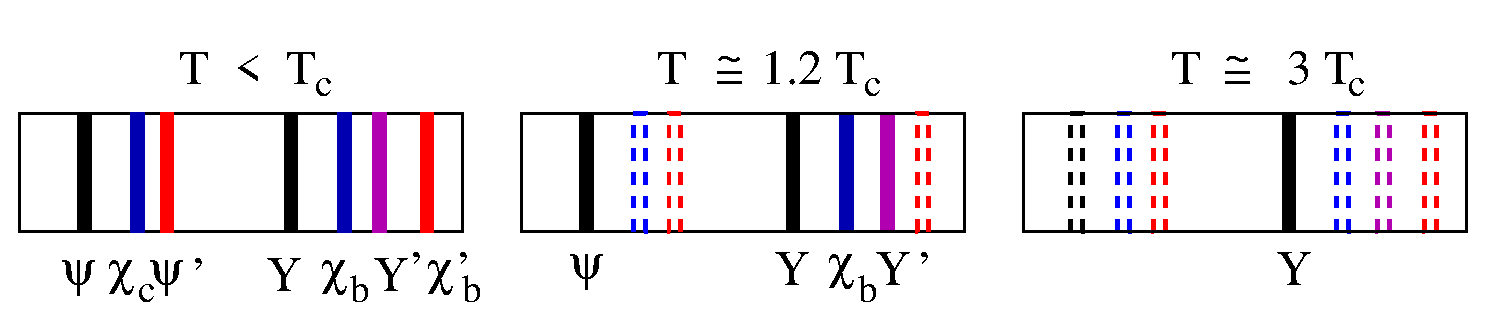
\includegraphics[width=.70\textwidth]{\imgpath/spec.eps}
\caption{Spectral lines corresponding to various charmonium and bottomonium states for different medium temperatures , relative to the QGP critical temperature. \cite{satzProbingStatesMatter2013}}
\label{fig:colls:thermometer}
\end{figure}

The production of heavy quarkonia in AA collisions is compared to that in pp collisions (scaled by the average number of binary collisions) through the nuclear modification factor, $R_{\mathrm{AA}}$. This quantity is widely used in various other measurements and is defined as:
\begin{align}
R_{\mathrm{AA}}=\frac{\mathrm{d}N_{\mathrm{AA}}/\mathrm{d}\pt}{\langle N_{\mathrm{coll}}\rangle\ \mathrm{d}N_{\mathrm{pp}}/\mathrm{d}\pt} \quad .
\end{align}
$R_{\mathrm{AA}}$ can take on the following values:
\begin{enumerate}
\item $R_\mathrm{AA} = 1$: The result one would expect if the AA collision is a mere superposition of nucleon-nucleon collisions. There is no net effect on the production, corresponding to the absence of the QGP medium and other nuclear effects, or their mutual cancellation.
\item $R_\mathrm{AA} < 1$: The production is overall suppressed, for example, due to dissociation.
\item $R_\mathrm{AA} > 1$: The plasma and nuclear effects systematically enhance the measured production.
\end{enumerate}

At LHC energies, the abundance of charm quarks in the QGP is high enough that charmonia can be formed after dissociation, which somewhat complicates the interpretation of charmonia suppression. However, the $\Upsilon(3\mathrm{S})$ bottomonium has $R_{\mathrm{AA}}$ consistent with zero at $\sqrt{s_{\mathrm{NN}}}=5.02$ TeV, as shown in Fig.~\ref{fig:colls:cmsupsilon} \cite{cmscollaborationMeasurementNuclearModification2019}. This complete suppression is a clear signature of the QGP and can be used together with models to estimate the QGP temperature at these energies as $T\approx 630$~MeV \cite{krouppaPredictionsBottomoniaSuppression2016}.

\begin{figure}[H]
\subfloat[][]{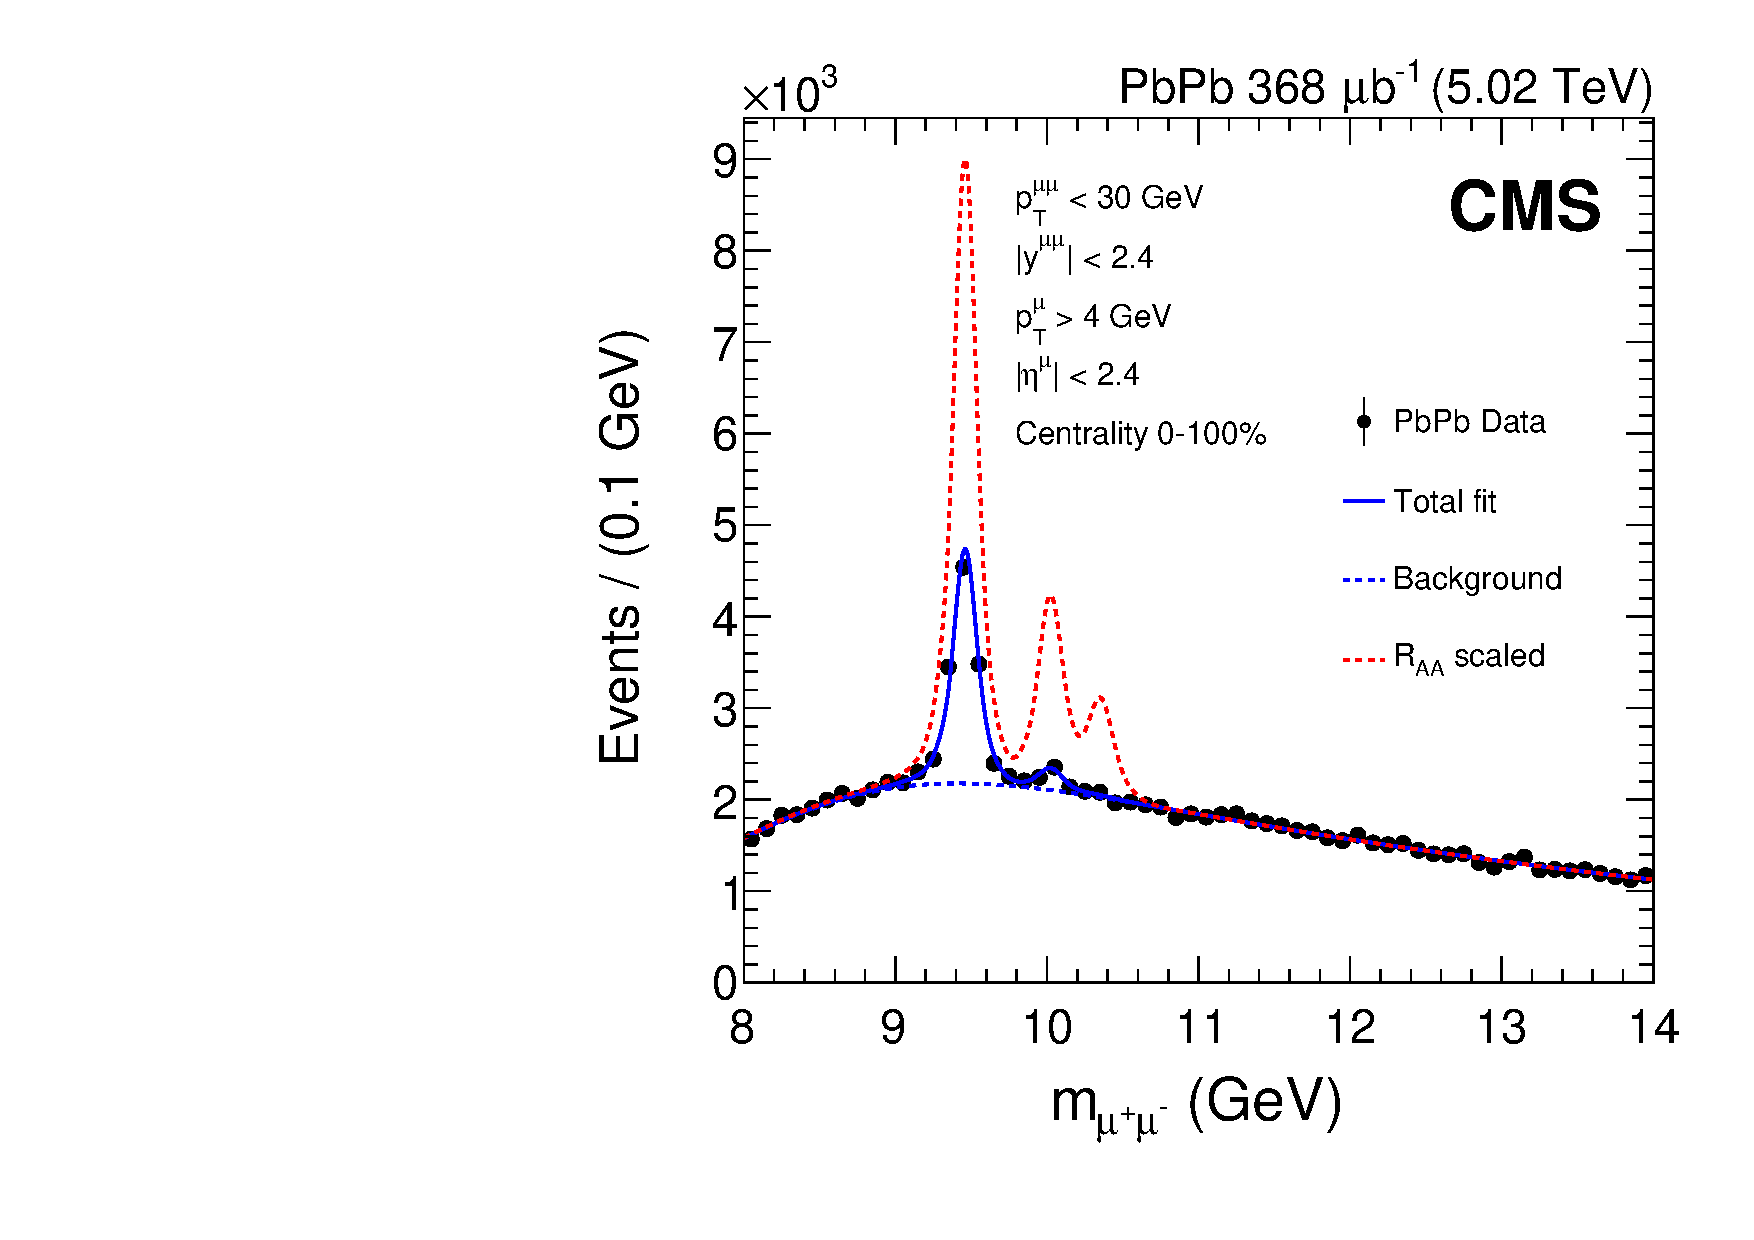
\includegraphics[width=.40\textwidth]{\imgpath/cms_ups1.pdf}}\hspace{2em} 
\subfloat[][]{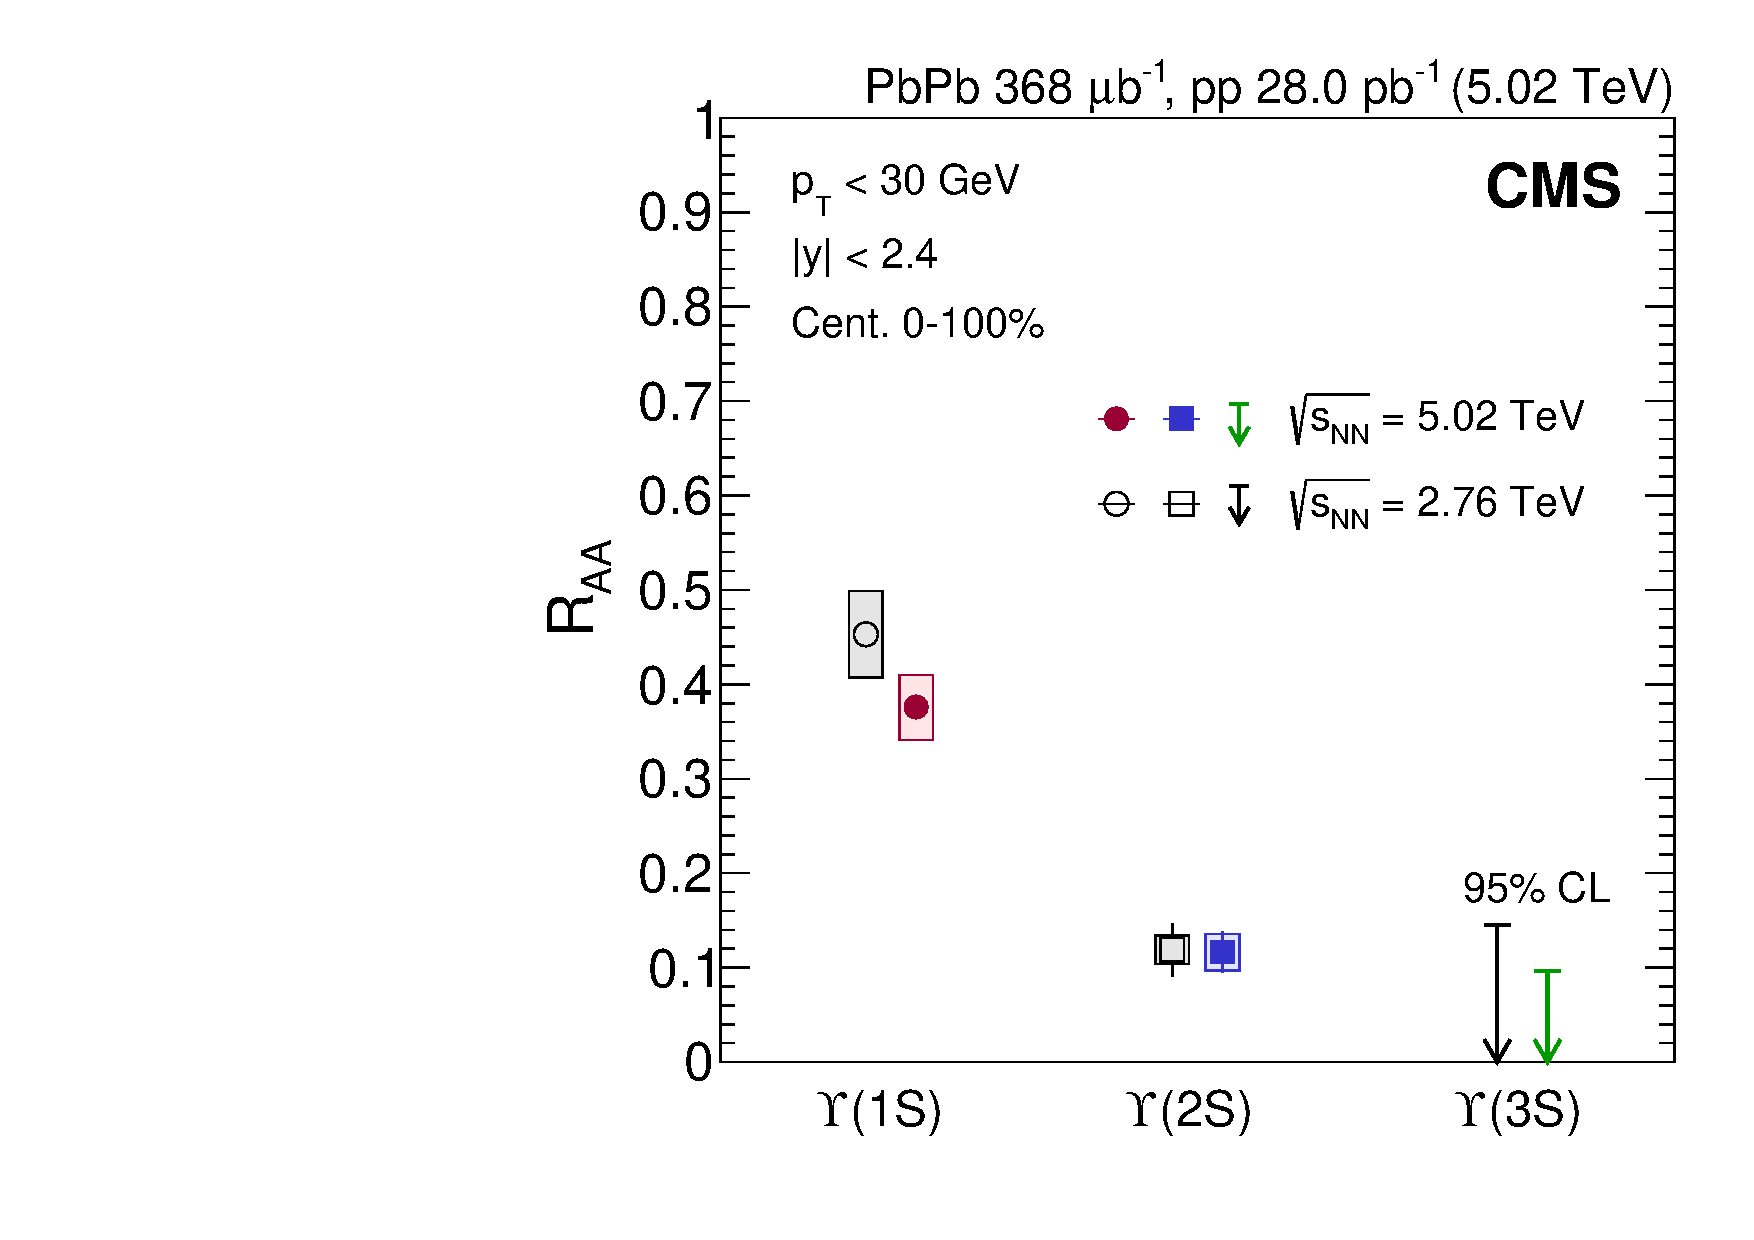
\includegraphics[width=.41\textwidth]{\imgpath/cms_ups2.pdf}}
\caption{\textbf{(a)} Muon invariant mass distributions in Pb-Pb collisions at \snnt{5.02}, also showing a scaled result from pp collisions at same energies (red dashed line). \textbf{(b)} Nuclear modification factors of the three bottomonium states. \cite{cmscollaborationMeasurementNuclearModification2019}}
\label{fig:colls:cmsupsilon}
\end{figure}

\subsection{Strangeness enhancement}

In the production of hadrons in vacuum, strangeness is suppressed relatively to light quarks not only due to the higher mass of the strange quark ($m_s \approx \gevcc{0.1}$), but also due to the much higher constituent mass ($m_K \approx \gevcc{0.5}$). However, in the QGP, due to the high gluon densities and $T\sim m_s$, strangeness production may equilibrate with $u$ and $d$ quarks through gluon fusion:
\begin{align*}
gg \to s\bar{s} \quad .
\end{align*}

This phenomenon was proposed as one of the first signatures of QGP observation in colliders \cite{rafelskiStrangenessProductionQuarkGluon1982, kochStrangenessRelativisticHeavy1986}. Indeed, an enhancement in the production of strange hadrons is observed in AA collisions, which is dependent on the event activity and increases with increasing strangeness content of the hadron \cite{alicecollaborationMultistrangeBaryonProduction2016}. Figure~\ref{fig:colls:strangeness} displays these results.

Furthermore, the yields of hadrons measured in AA collisions can be accurately described by statistical models \cite{andronicThermalHadronProduction2009, wheatonTHERMUSThermalModel2009} which, generally, assume that the dense system is in thermal and chemical equilibrium at the point of its freeze-out. In these models, strangeness is assumed to be conserved on average, which corresponds to a grand-canonical ensemble with a strange chemical potential $\mu_S$. 

In small systems, the conservation of strangeness must be taken into account for each interaction, locally. This necessitates the use of a canonical ensemble and introducing a parameter, $V_0$, to describe the volume of this locality requirement \cite{hamiehCanonicalDescriptionStrangeness2000}. With this approach, strangeness enhancement can be reproduced by increasing $V_0$ and transitioning from the canonical ensemble in small systems to the grand-canonical ensemble in AA collisions, as depicted in Fig.~\ref{fig:colls:strangeness}.

\begin{figure}[H]
\subfloat[][]{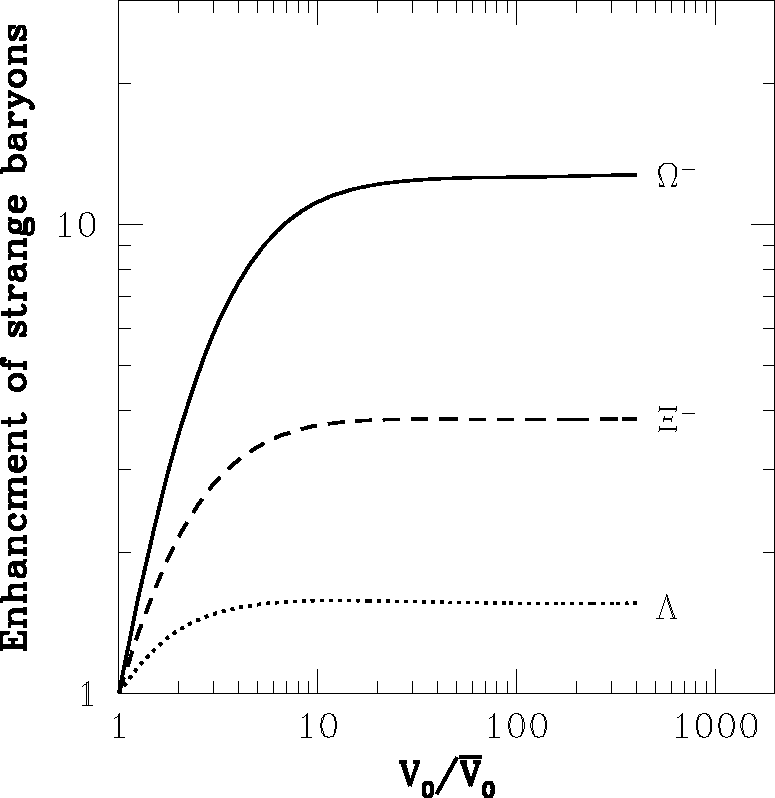
\includegraphics[height=11.85em]{\imgpath/se_v02.pdf}}\hspace{1em}
\subfloat[][]{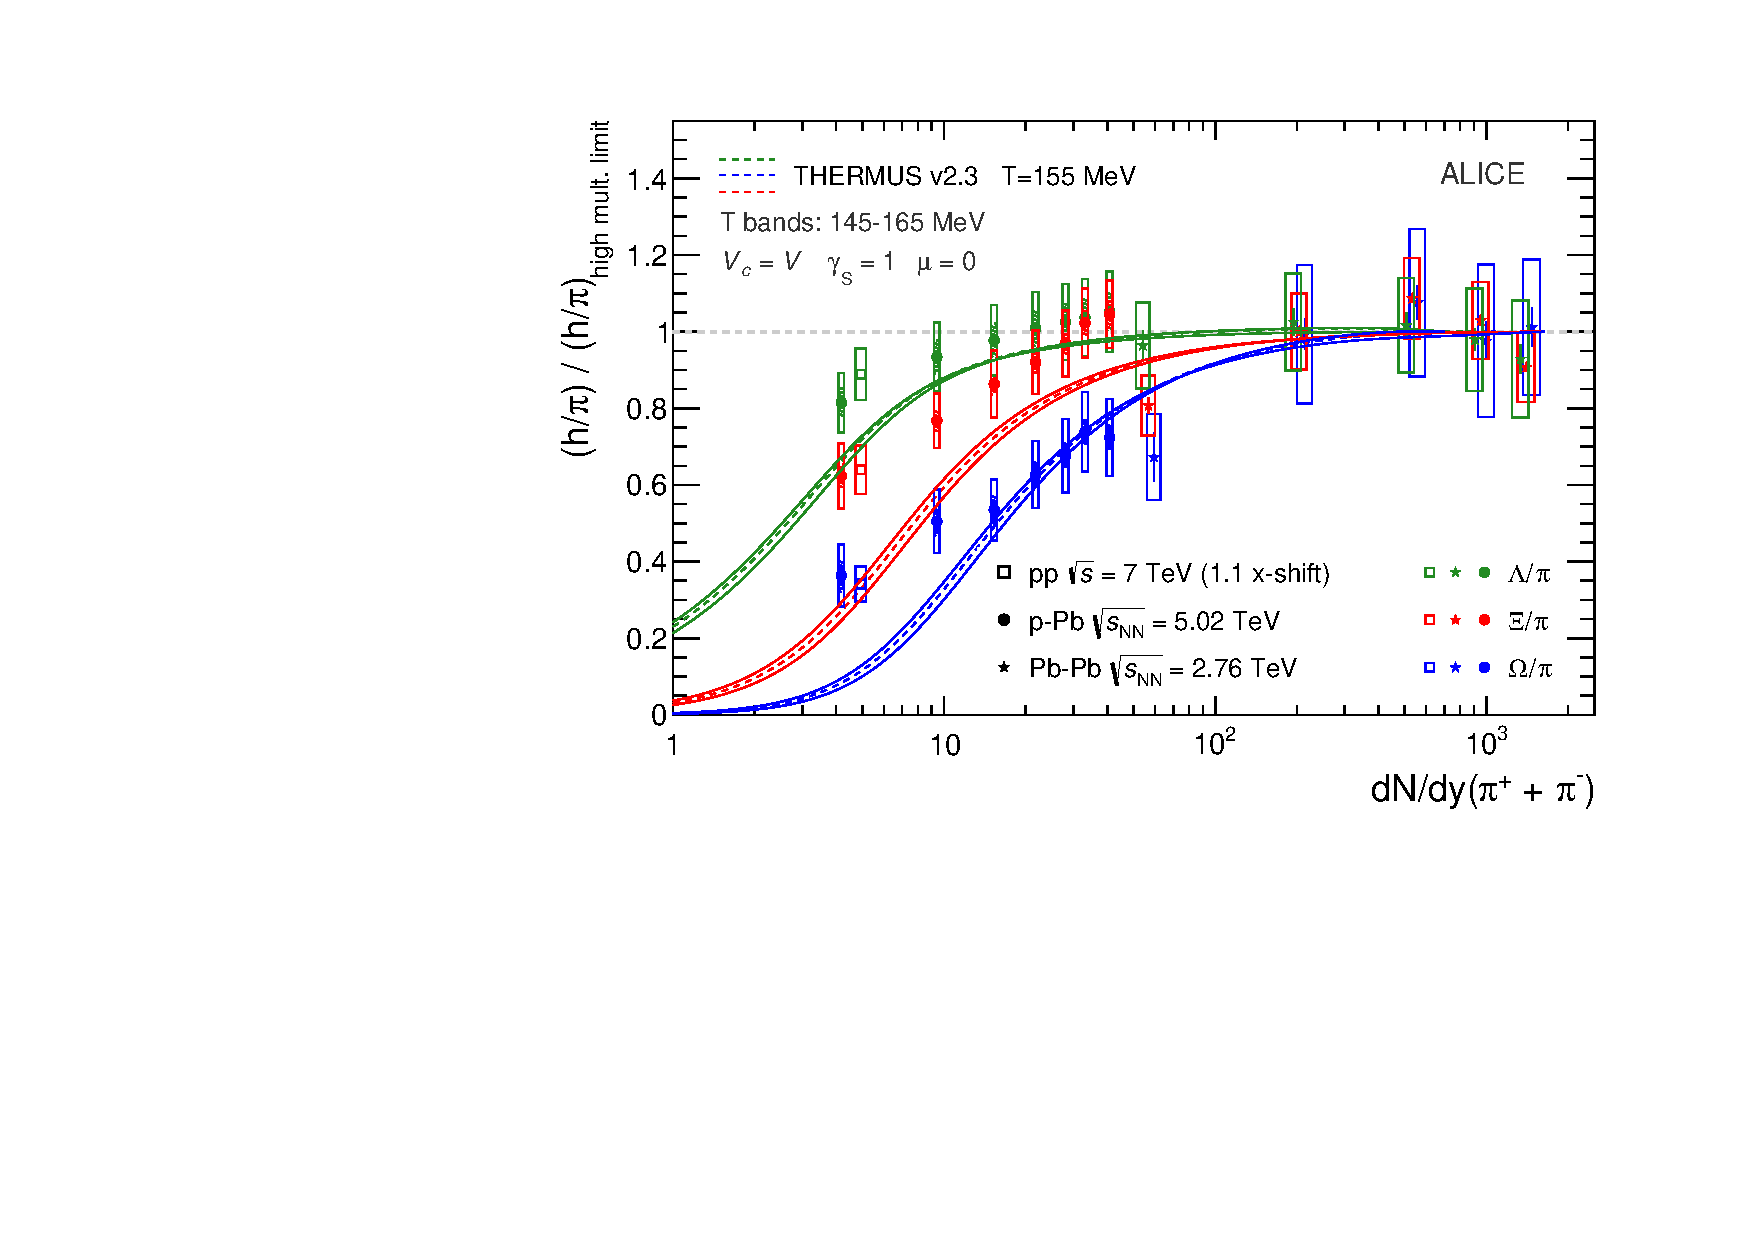
\includegraphics[height=13em]{\imgpath/se_omegaxi.pdf}}
\caption{\textbf{(a)} Dependence of strange baryon densities on the parameter $V_0$ characterising the volume where strangeness is locally conserved in models describing strangeness suppression in small systems as canonical suppression. The volume is normalised to a typical AA value of $\overline{V}_0=7.4$~fm$^{3}$. \cite{hamiehCanonicalDescriptionStrangeness2000}. \textbf{(b)} Ratios of yields of strange baryons to pions in pp, p-Pb, and Pb-Pb collisions as a function of the pion multiplicity normalised to the high-multiplicity limit in $0-60\%$ most central Pb-Pb collisions. The results are compared with a statistical model combining the canonical and grand-canonical approach. \cite{alicecollaborationMultistrangeBaryonProduction2016, wheatonTHERMUSThermalModel2009}}
\label{fig:colls:strangeness}
\end{figure}

%\begin{figure}[H]
%\subfloat[][]{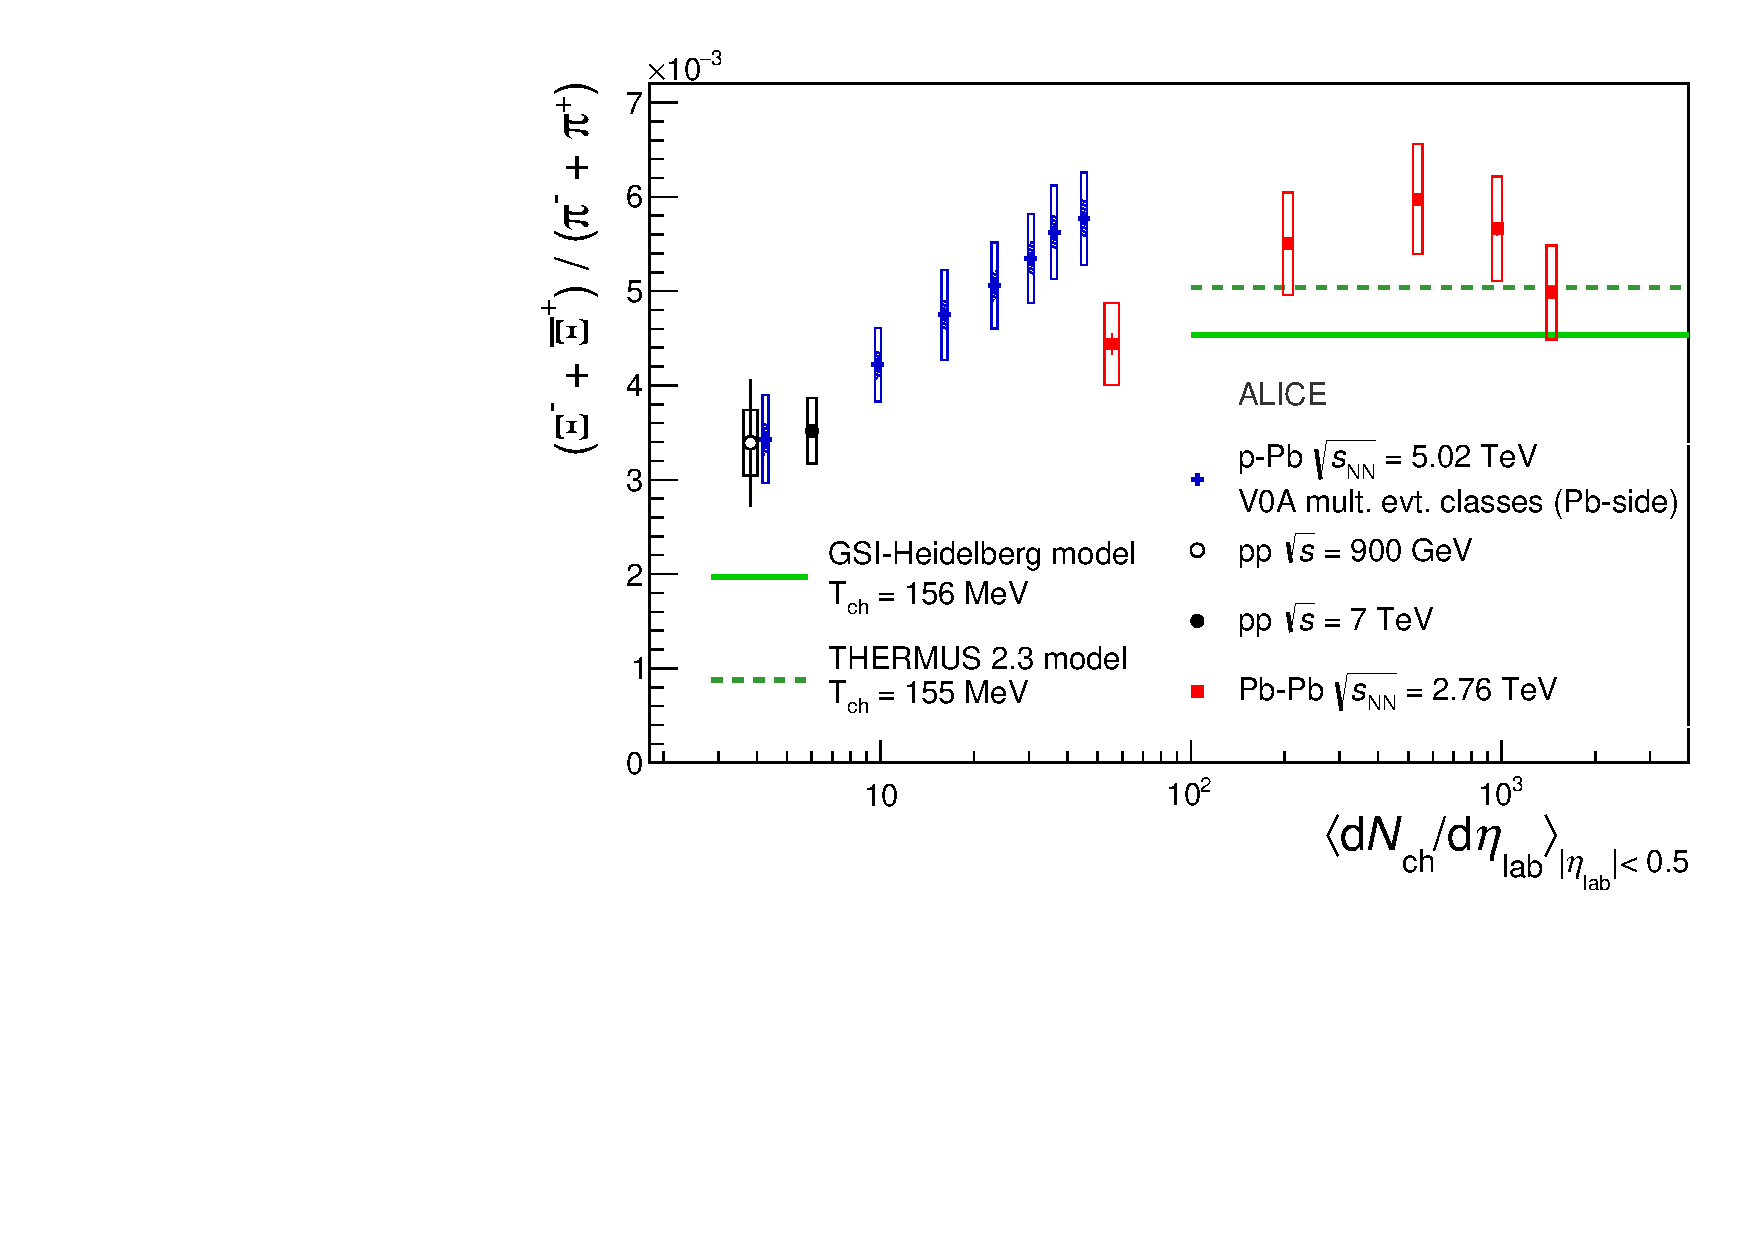
\includegraphics[width=.47\textwidth]{\imgpath/xitopi.pdf}}\hspace{1em}
%\subfloat[][]{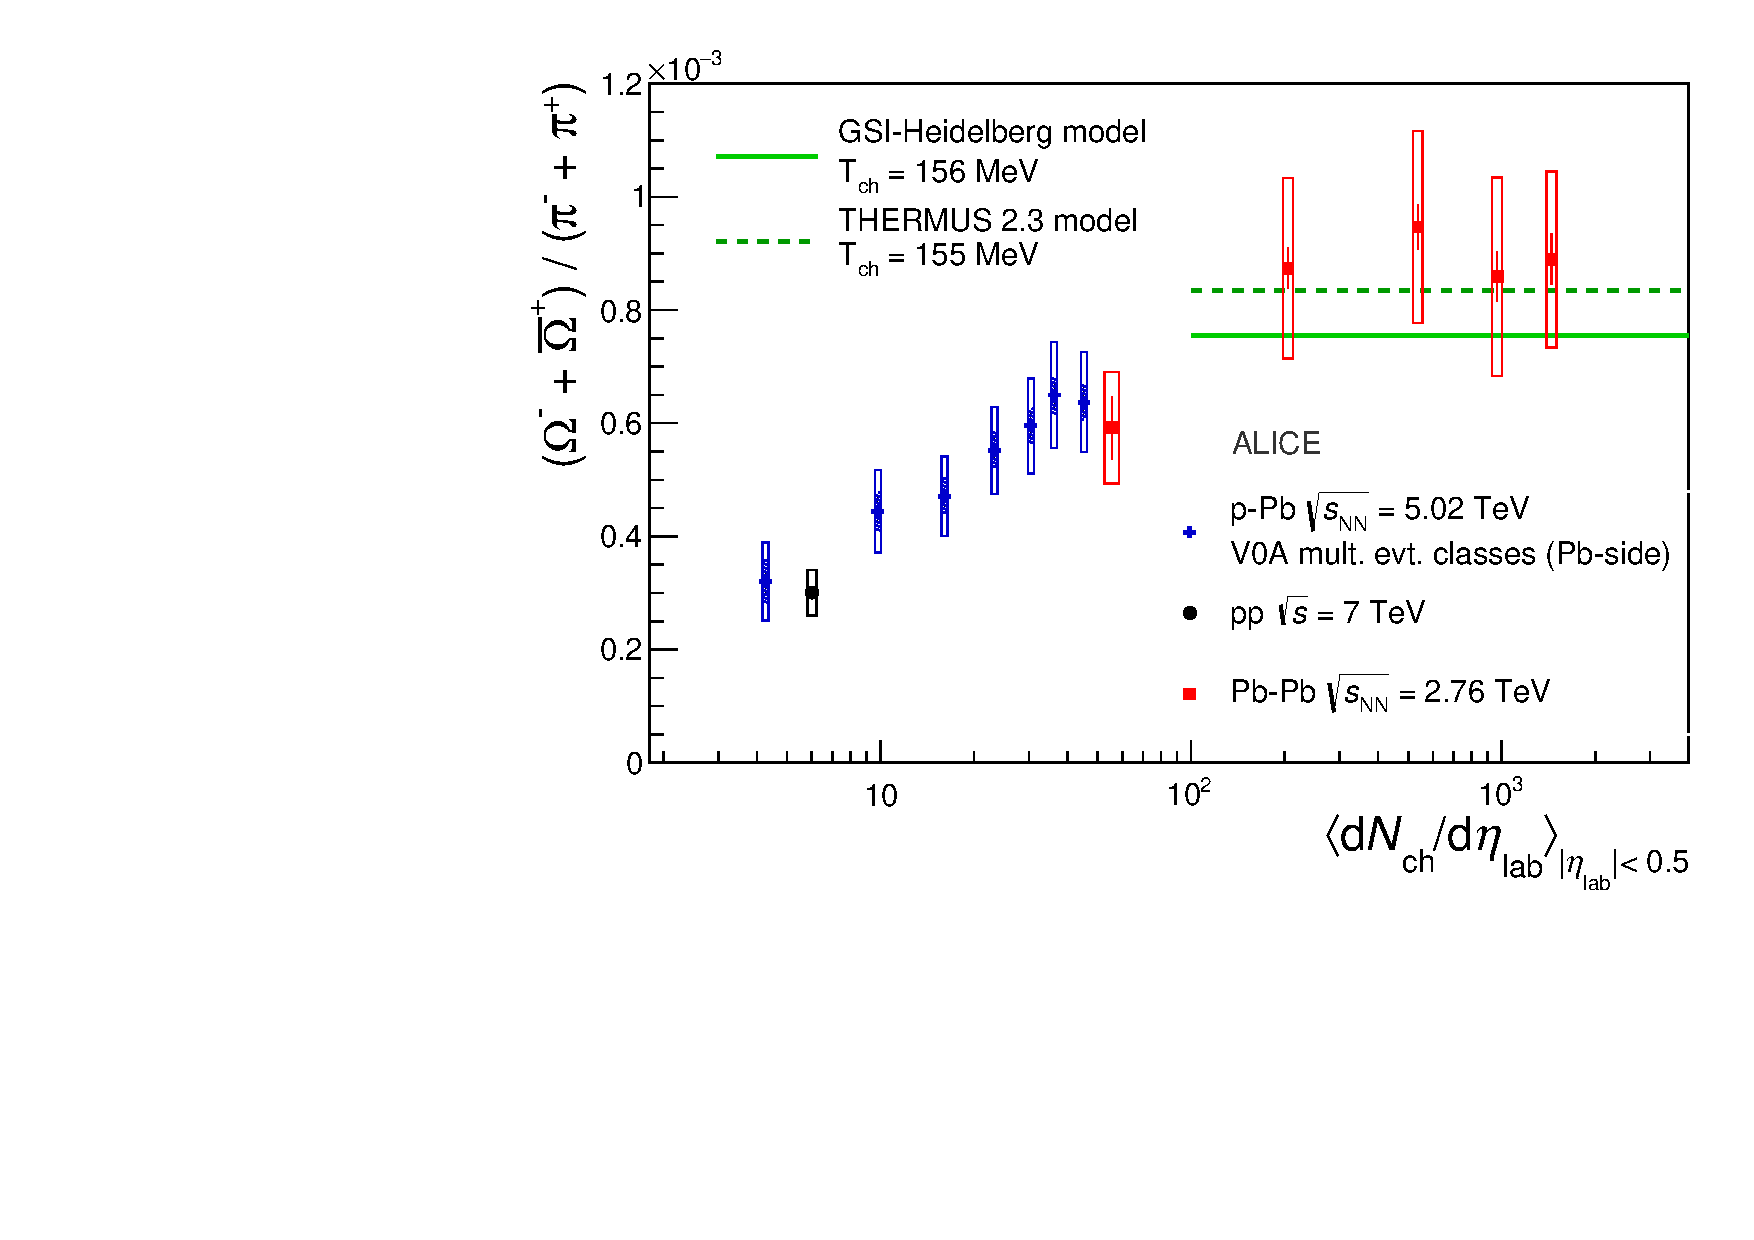
\includegraphics[width=.47\textwidth]{\imgpath/omegatopi.pdf}}
%\caption{TBA}
%\label{fig:colls:strangeness}
%\end{figure}

\subsection{Collective flow}

The strongly interacting plasma exhibits a collective expansion which can be described by hydrodynamic equations, since the mean free paths of the constituents are much smaller than the system size ($\lambda \ll L$). The non-uniform energy density in the initial state results in varying pressure gradients, which drive this expansion. Since the centre of the plasma has greater pressure than its outside regions, common expansion velocity field develops, which results in the so-called \textit{radial flow}. Similarly, the medium also translates the directionally-dependent anisotropies in the initial state, which stem from the almond-shape geometry of the collision overlap region as well as nucleonic fluctuations, to the final-state. This is the so-called \textit{anisotropic flow}.

Together with hadronic re-scattering, the flows are reflected in the kinematics of the final-state hadrons. When comparing \pt spectra in central AA collisions to those in peripheral or in pp collisions, a broadening as well as a momentum boost can be observed (see Fig.~\ref{fig:colls:rflow}), caused by the radial expansion as well as the less important thermal motion \cite{alicecollaborationCentralityDependenceRm2013, alicecollaborationRmSRm2013, alicecollaboration8920Phi2015}. The expansion effect depends on the mass of the hadrons, as the amount of additional \pt acquired is proportional to their mass and the collective expansion velocity field, $p \approx m\beta c$. A notable exception to this trend is the $\phi$ quarkonium; although comparable with the proton ($m_\phi \approx \gevcc{1.02} \sim m_p$), its scattering cross-section is much smaller \cite{hungEquationStateRadial1998}.

The \pt spectra influenced by radial flow can be described by the Blast-Wave parametrisation \cite{schnedermannThermalPhenomenologyHadrons1993}. In this approach, the radial expansion is accounted for as a common velocity field profile $\beta (r)$ affecting thermal spectra, 

\begin{minipage}{0.5\linewidth}
    \begin{center}
        \begin{tikzpicture}
            \draw[->] (-0.25,0) -- (2.5,0) node[right] {$r$};
            \draw[->] (0,-0.2) -- (0,1.2) node[above] {$\beta(r)$};
            \draw[scale=1,domain=0.0:2.2,smooth,variable=\x,blue] plot ({\x},{0.95*(\x/2.2)^0.7});
            \draw[dashed] (2.2,0) node[below] {$R$} -- (2.2,1);
        \end{tikzpicture}
    \end{center}
\end{minipage}%
\begin{minipage}{0.5\linewidth}
    \begin{equation}
		\beta (r) = \beta_s (\frac{r}{R})^n \quad ,
    \end{equation}
\end{minipage}

where $\beta_s$, $R$, and $n$ are the expansion velocity on the surface of the plasma, its radius, and an extra parameter usually ranging $0.7-1.0$ in central collisions \cite{alicecollaborationCentralityDependenceRm2013}, respectively. The effects of radial flow can also be reproduced in AA collisions with hydrodynamic models using an equation of state from LQCD and hadronic re-scattering \cite{hungEquationStateRadial1998}, and in pA collisions with the EPOS3 model, which also incorporates hydrodynamic evolution in QGP droplets \cite{wernerAnalysingRadialFlow2014}.

Ratios of baryons to mesons, such as $p/\pi$ or \ltok, as a function of event activity are often used to demonstrate the effect of radial flow, as shown in Fig.~\ref{fig:colls:rflow}. In these ratios, the modification of \pt spectra results in the following effects on the high-event-activity ratios:
\begin{enumerate}
\item The peak in the ratio is shifted to higher \pt by up to $\gevc{1.5}$,
\item there is an enhancement of baryons in the intermediate \pt $1.5 < \pt < \gevc{6}$ region,
\item and a corresponding depletion of baryons at low \pt.
\end{enumerate}

Figure~\ref{fig:colls:aflow} shows a typical shape of the initial state with its azimuthal anisotropy and the resulting pressure gradients. Anisotropic flow can be quantified by decomposing the azimuthal particle distribution into its Fourier series \cite{voloshinFlowStudyRelativistic1996}:
\begin{align}
\frac{dN}{d\varphi} \propto 1 + 2 \sum_{n=1}^{\infty} v_n e^{in(\varphi - \Psi_n)} \, , \quad \ v_n = \langle\cos[n(\phi - \Psi_n)]\rangle \, ,
\end{align}
where $\Psi_n$ is the symmetry plane of the $n$-th harmonic and $v_n$ is the Fourier coefficient corresponding to that harmonic, also known as the flow coefficient. In this context, a finite initial state ellipticity $\epsilon_2$ leads to a finite \textit{elliptic flow} $v_2$, triangularity $\epsilon_3$ to a \textit{triangular flow} $v_3$, and so on \cite{alverCollisionGeometryFluctuations2010, alicecollaborationHigherHarmonicAnisotropic2011}. 

\begin{figure}[H]
\subfloat[][]{\adjustbox{valign=m}{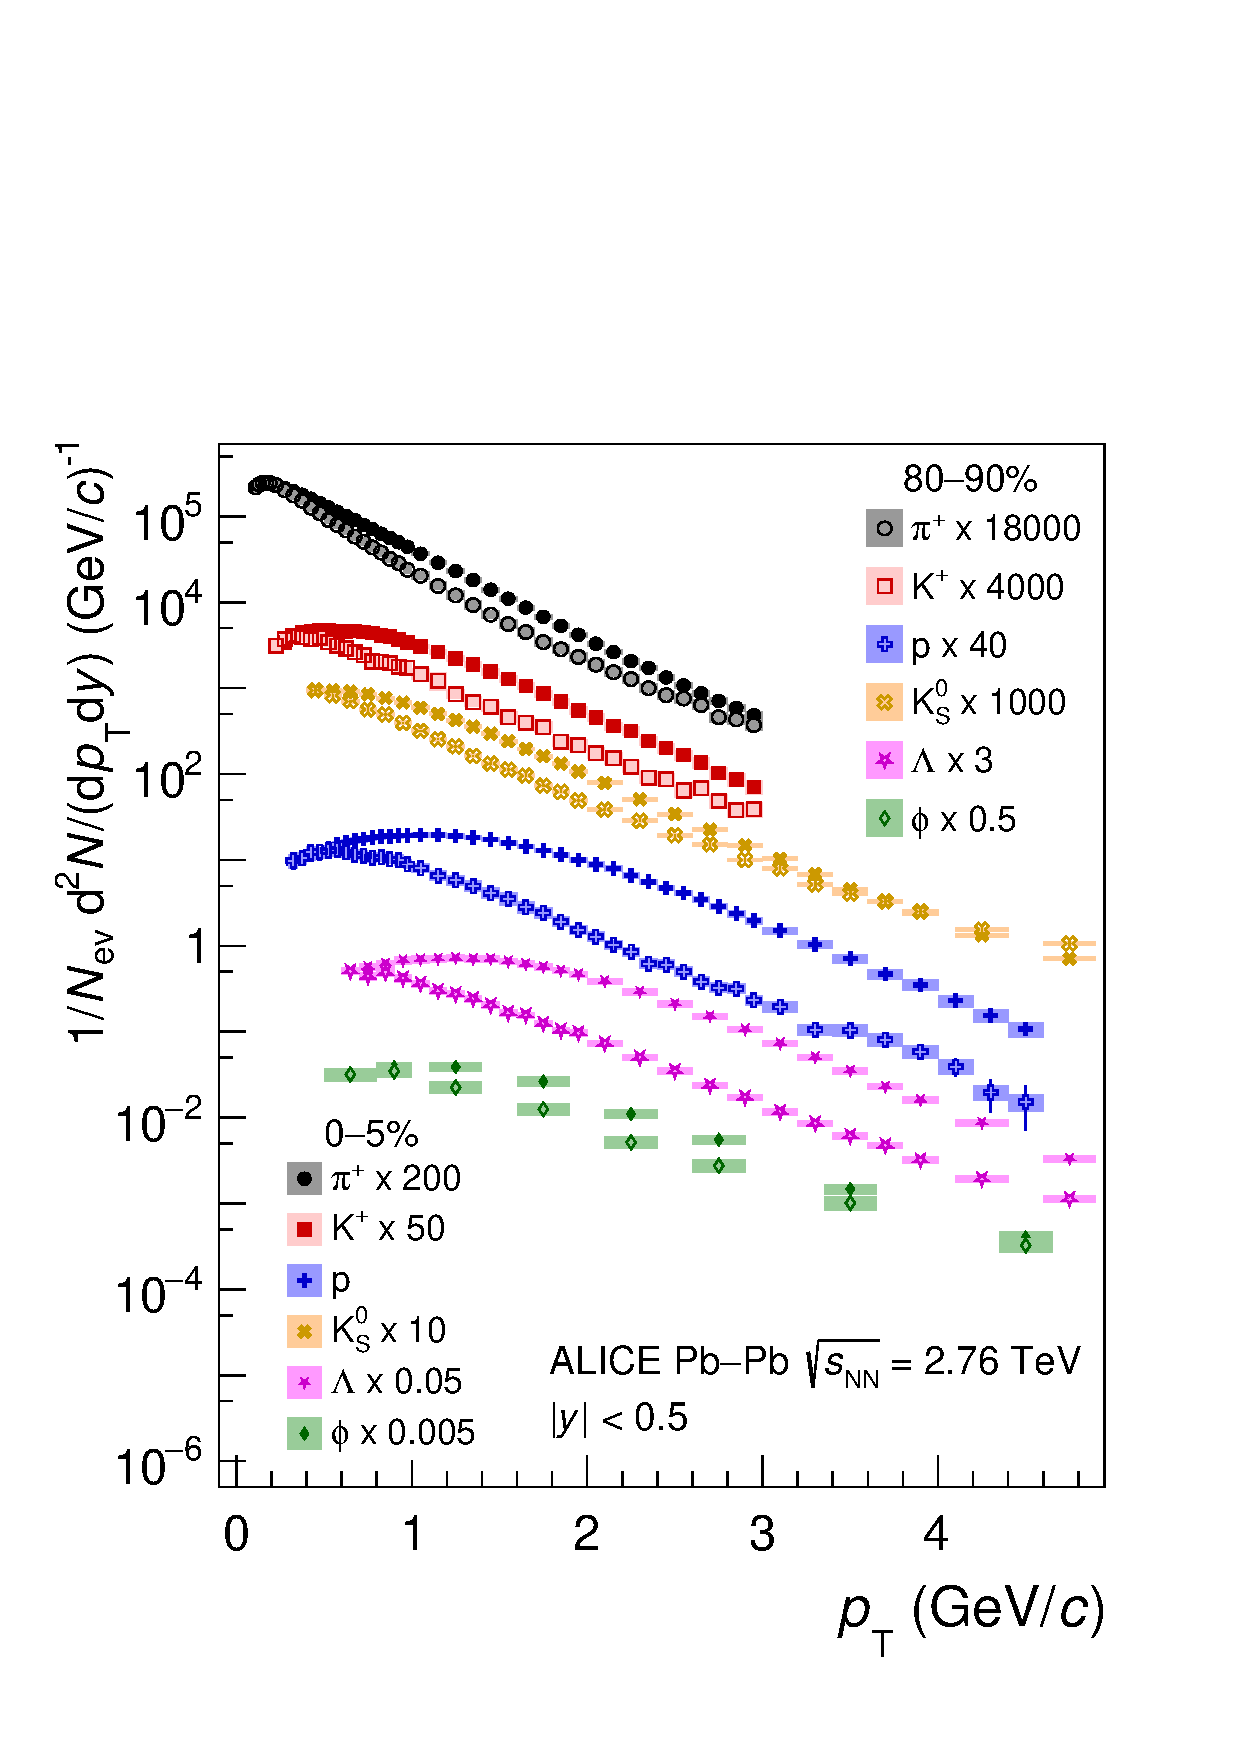
\includegraphics[width=.4\textwidth]{\imgpath/rfspectra.pdf}}}%\hspace{2em}
\subfloat[][]{\adjustbox{valign=m}{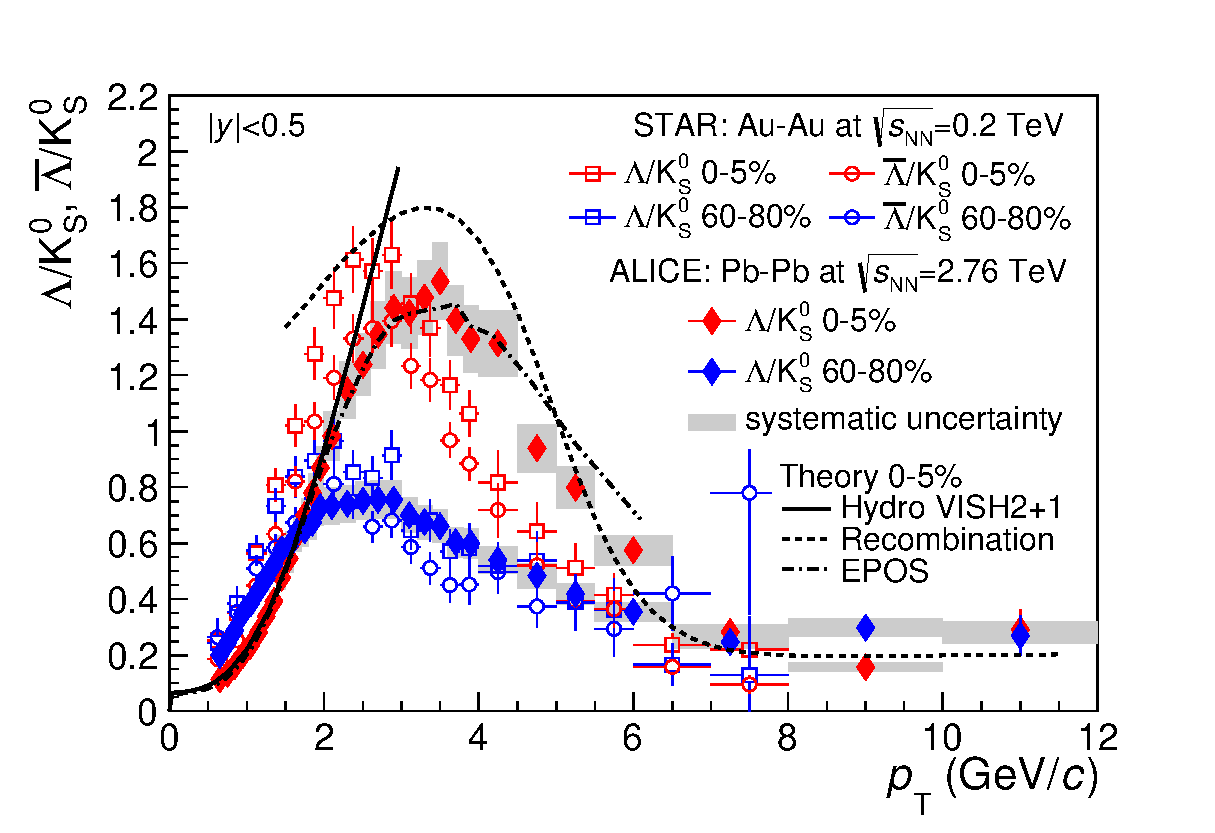
\includegraphics[width=.59\textwidth]{\imgpath/ltok.eps}}}
\caption{\textbf{(a)} Transverse momentum spectra of light-flavour hadrons in central $0-5\%$ and peripheral $80-90\%$ Pb-Pb collisions scaled by arbitrary factors to enhance the visibility. \cite{alicecollaborationALICEExperimentJourney2022, alicecollaborationCentralityDependenceRm2013, alicecollaborationRmSRm2013, alicecollaboration8920Phi2015} \textbf{(b)} \LA to \KOs ratios of transverse momentum spectra in Pb-Pb collisions at the LHC and Au-Au collisions at RHIC for central $0-5\%$ events (red) and peripheral $60-80\%$ events (blue). \cite{alicecollaborationRmSRm2013}}
\label{fig:colls:rflow}
\end{figure}

The flow coefficients can be experimentally extracted using various methods, including two-particle azimuthal correlations (as shown in Fig.~\ref{fig:colls:aflow}), and are typically studied as a function of event multiplicity. It is important to note that these azimuthal correlations between particles due to anisotropic flow are long-range, i.e.\ present consistently across the entire pseudorapidity range $\Delta \eta$ (the so-called ``ridge") \cite{luzumFlowFluctuationsLongrange2011}, which makes them distinguishable from similarly appearing ``non-flow" short-range correlations coming from jet fragmentation and resonance decays.
 
Moreover, measurements of $v_2$ in AA collisions for different particle species reveal a mass dependence in the low-\pt region, and a baryon/meson dependence in the intermediate \pt region, with baryons having approximately $1.5$ times higher values \cite{alicecollaborationEllipticFlowIdentified2015}. This suggests that the flow of hadrons is built up from its deconfined constituents.

\begin{figure}[H]
\subfloat[][]{\adjustbox{valign=m}{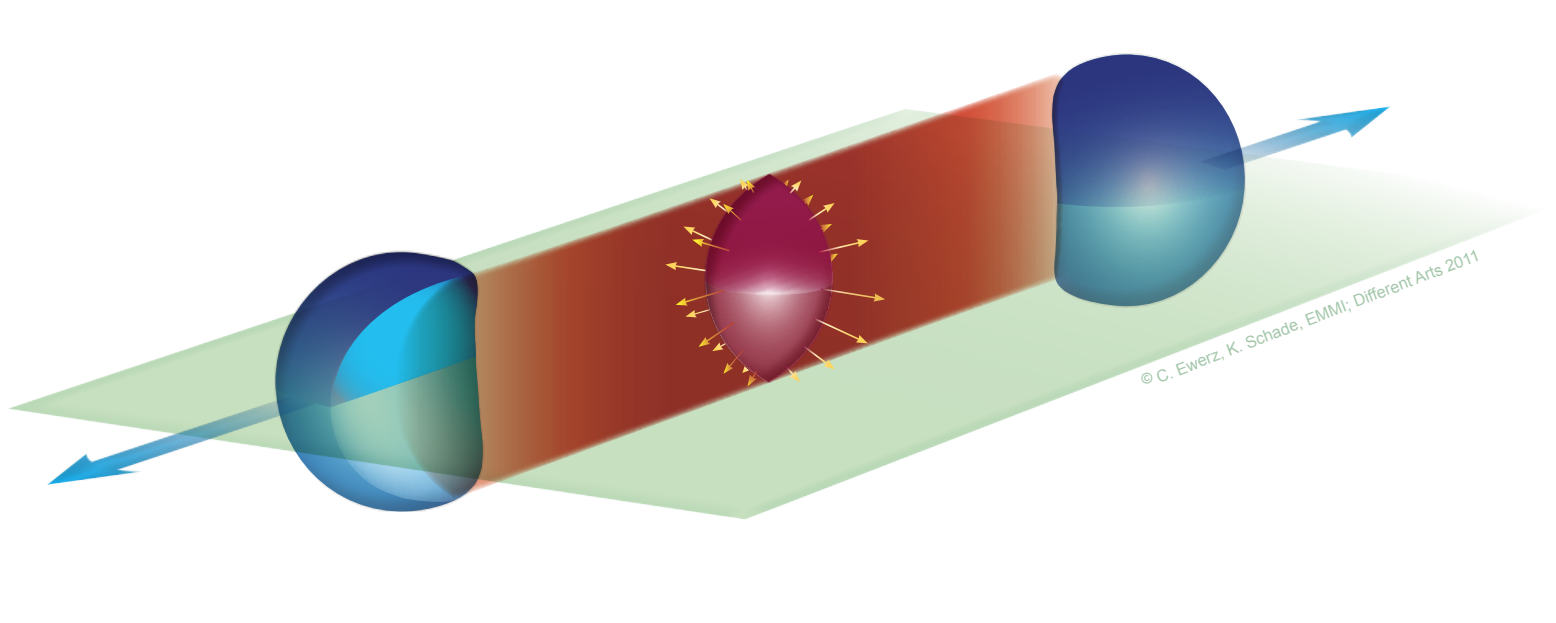
\includegraphics[width=.45\textwidth]{\imgpath/almond.png}}}\hspace{1em}
\subfloat[][]{\adjustbox{valign=m}{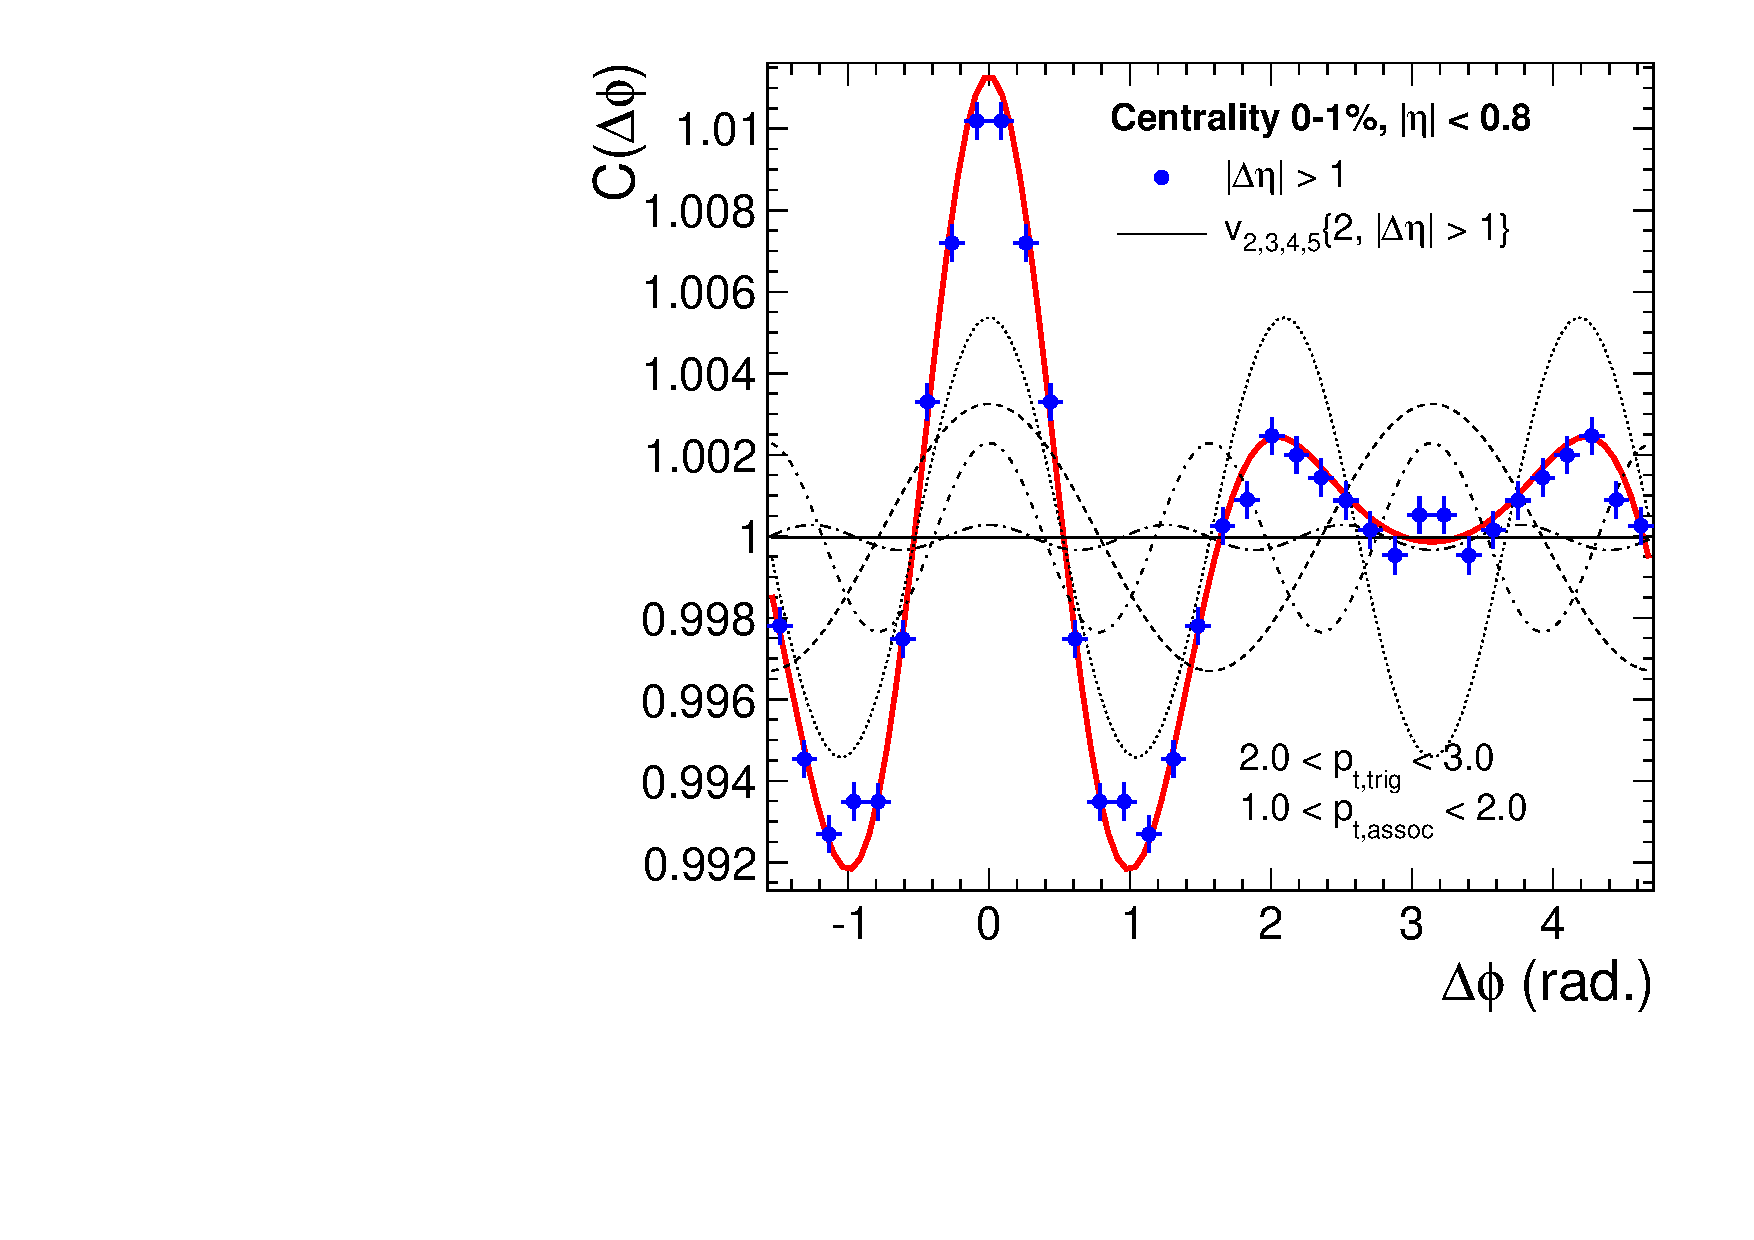
\includegraphics[width=.45\textwidth]{\imgpath/harmonics.pdf}}}
\caption{\textbf{(a)} Illustration of a collision of ultra-relativistic heavy nuclei and the overlapping region with pressure gradients (yellow). \cite{schadeApplicationsHolographyStrongly2012} \textbf{(b)} Correlation function of the relative azimuthal angle between a trigger particle and an associated particle, separated by a pseudorapidity gap, measured in central Pb-Pb collisions. The contributions from the elliptical, triangular, quadrupolar, and pentapolar harmonics are shown as different dashed lines. \cite{alicecollaborationHigherHarmonicAnisotropic2011}}
\label{fig:colls:aflow}
\end{figure}

\subsection{Jet quenching}

In AA collisions, partons produced in hard scattering processes interact with the colour charges in the quark-gluon plasma, resulting in the loss of energy through collisions and gluon bremstsstrahlung. This phenomenon is known as jet quenching and modifies or even "quenches" the parton shower \cite{gyulassyJetQuenchingDense1990, wangEffectJetQuenching1998}. In the factorisation theorem in Eq.~\ref{eq:intro:facto}, this corresponds to the medium-modification of the fragmentation functions. Studies of parton energy loss and jet quenching often use the transport coefficient $\hat{q}$, which describes the average \pt loss of a parton per a mean free path in the plasma and corresponds to the medium opacity

Jet quenching is one of the most important probes into the structure and dynamical properties of the QGP, since the hard partons experience its entire evolution, similarly to the case of heavy quarkonia discussed in Sec.~\ref{sec:colls:quarkonia}. It can also be compared with a large body of sound theoretical calculations \cite{gyulassyNonAbelianEnergyLoss2000} and MC simulations \cite{zappMonteCarloModel2009} based on QCD. Experimentally, jet quenching can manifest as suppression of the jet yield or even its complete disappearence, due to the energy loss of partons in the medium and their re-scattering. \cite{alicecollaborationALICEExperimentJourney2022}

Figure~\ref{fig:colls:jetquenching} displays such an AA event with a large jet imbalance and juxtaposes it with a pp event, where the leading and the recoil jet need to be balanced in azimuth due to conservation laws. Further effects and fields of study of jet quenching include the modification of jet substructures and shapes.

\begin{figure}[H]
\subfloat[][]{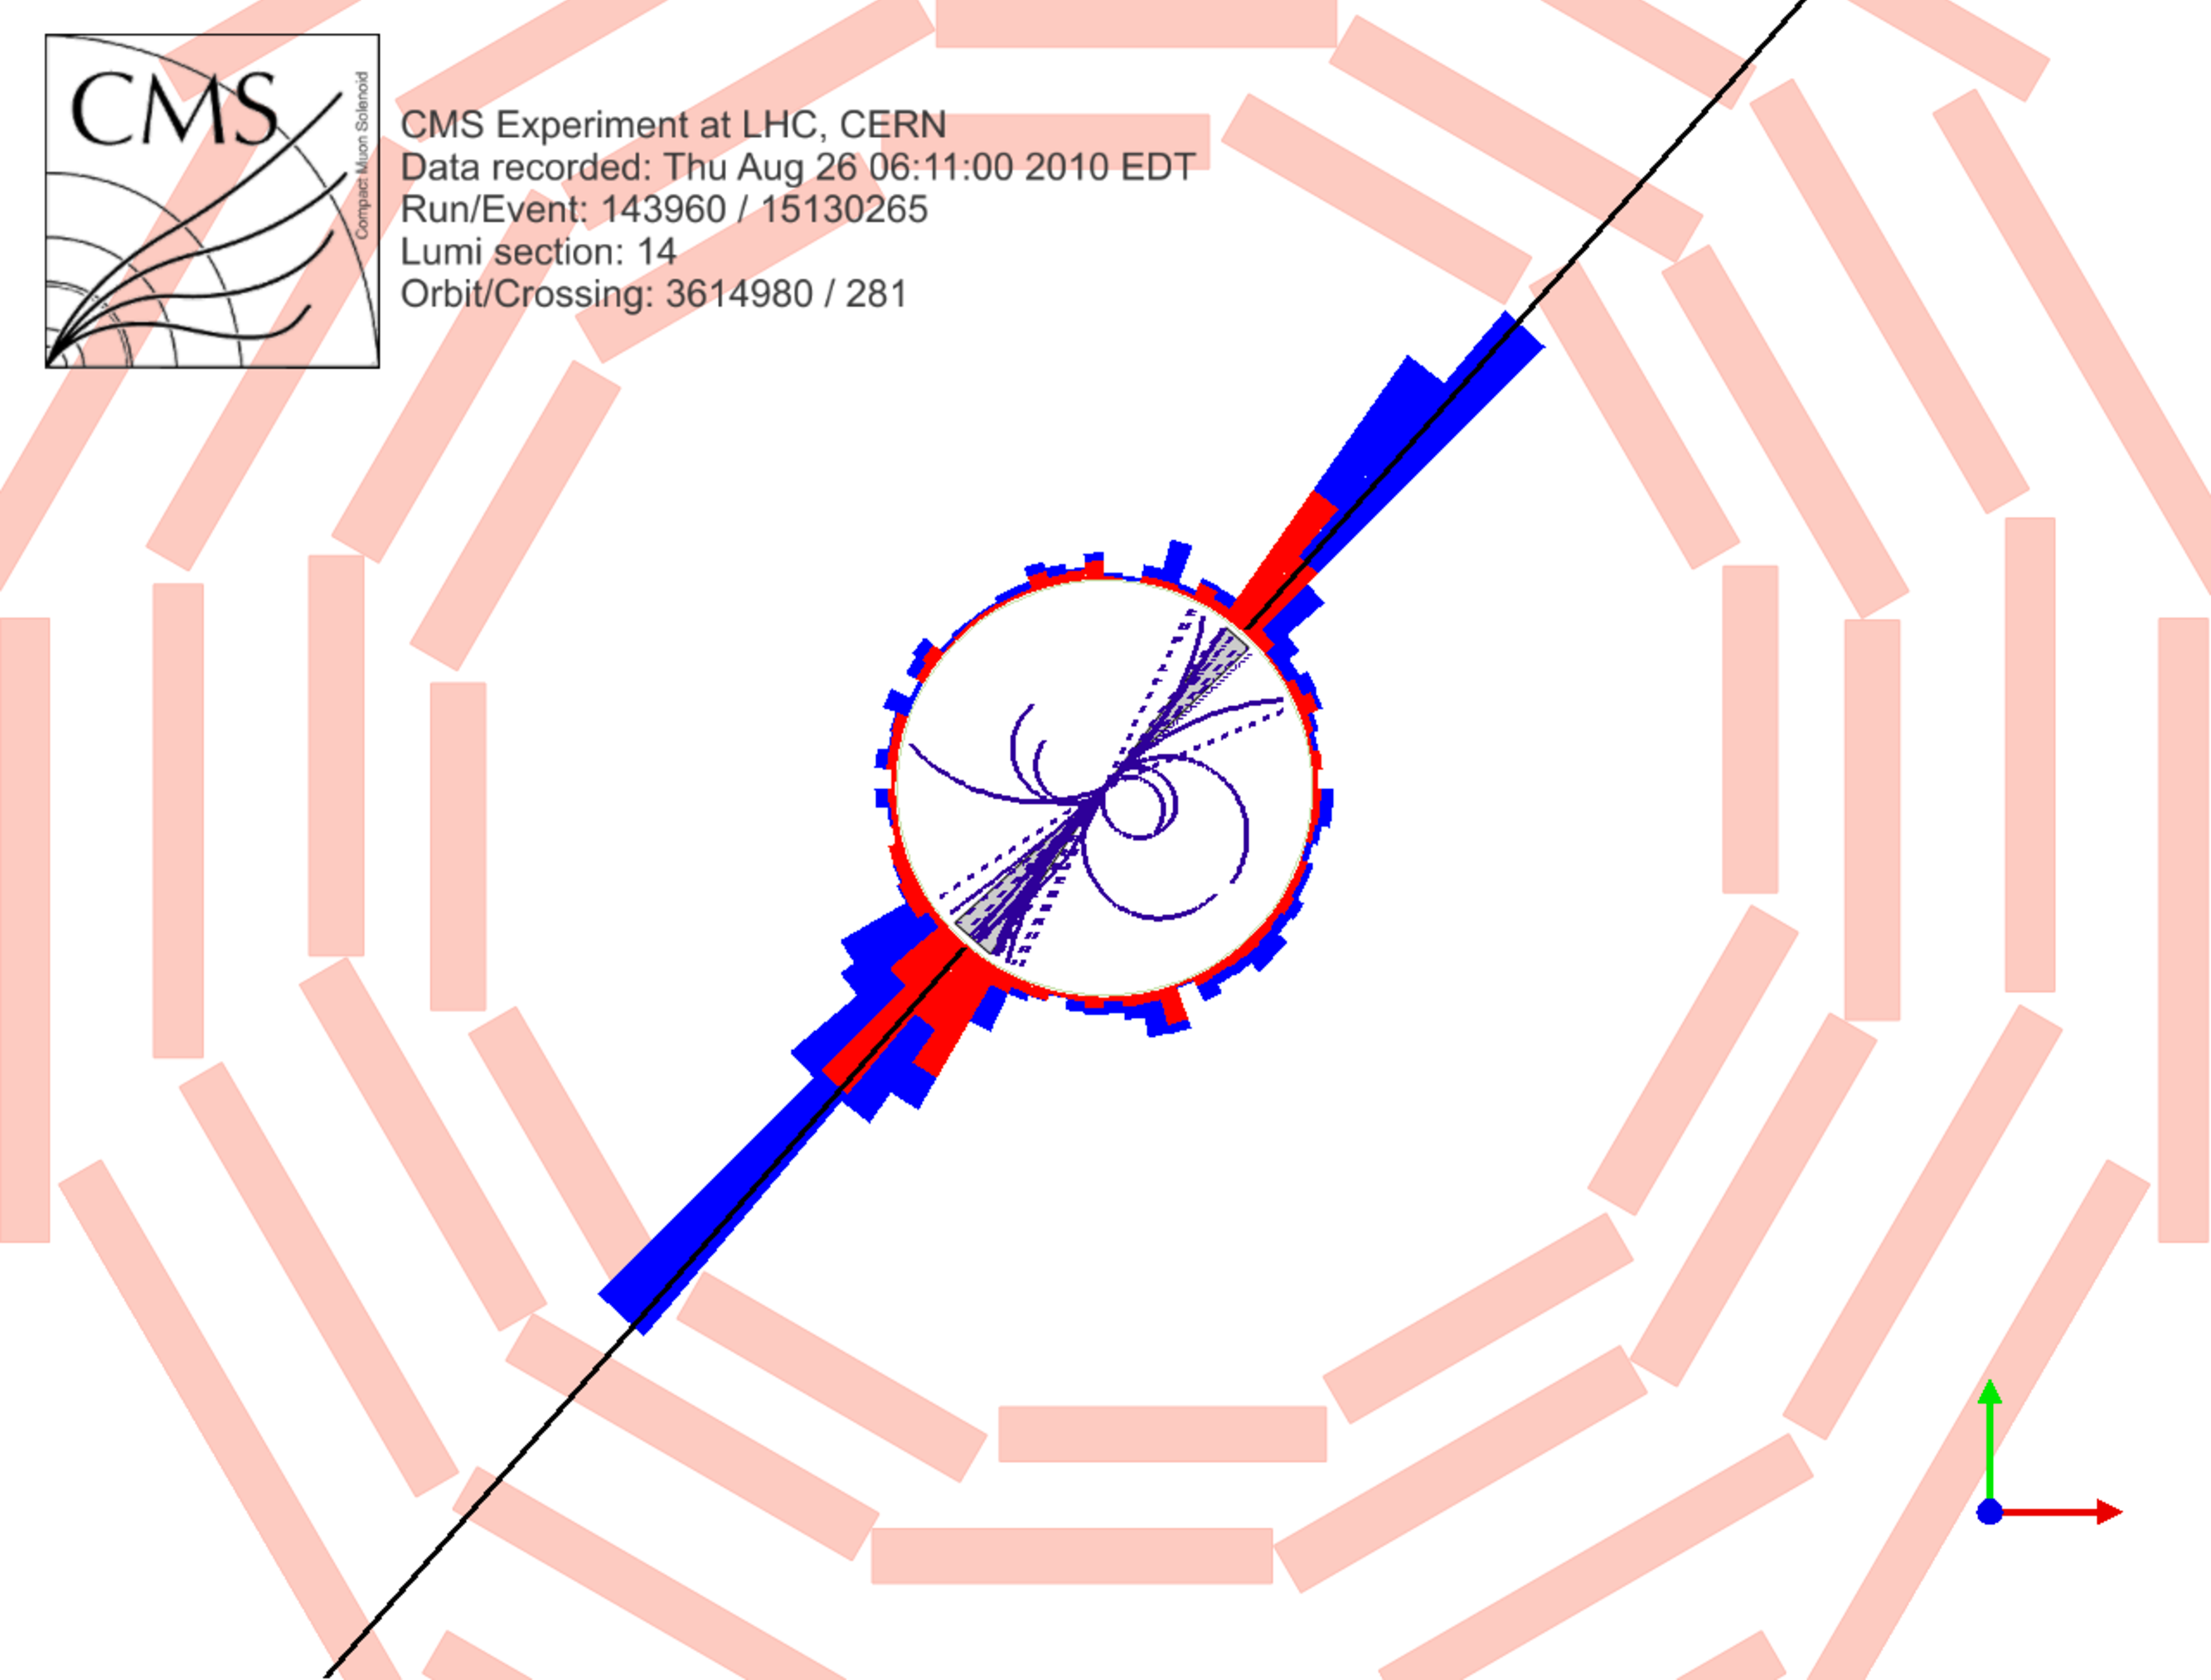
\includegraphics[height=11em]{\imgpath/DijetPP.pdf}}\hspace{2em} 
\subfloat[][]{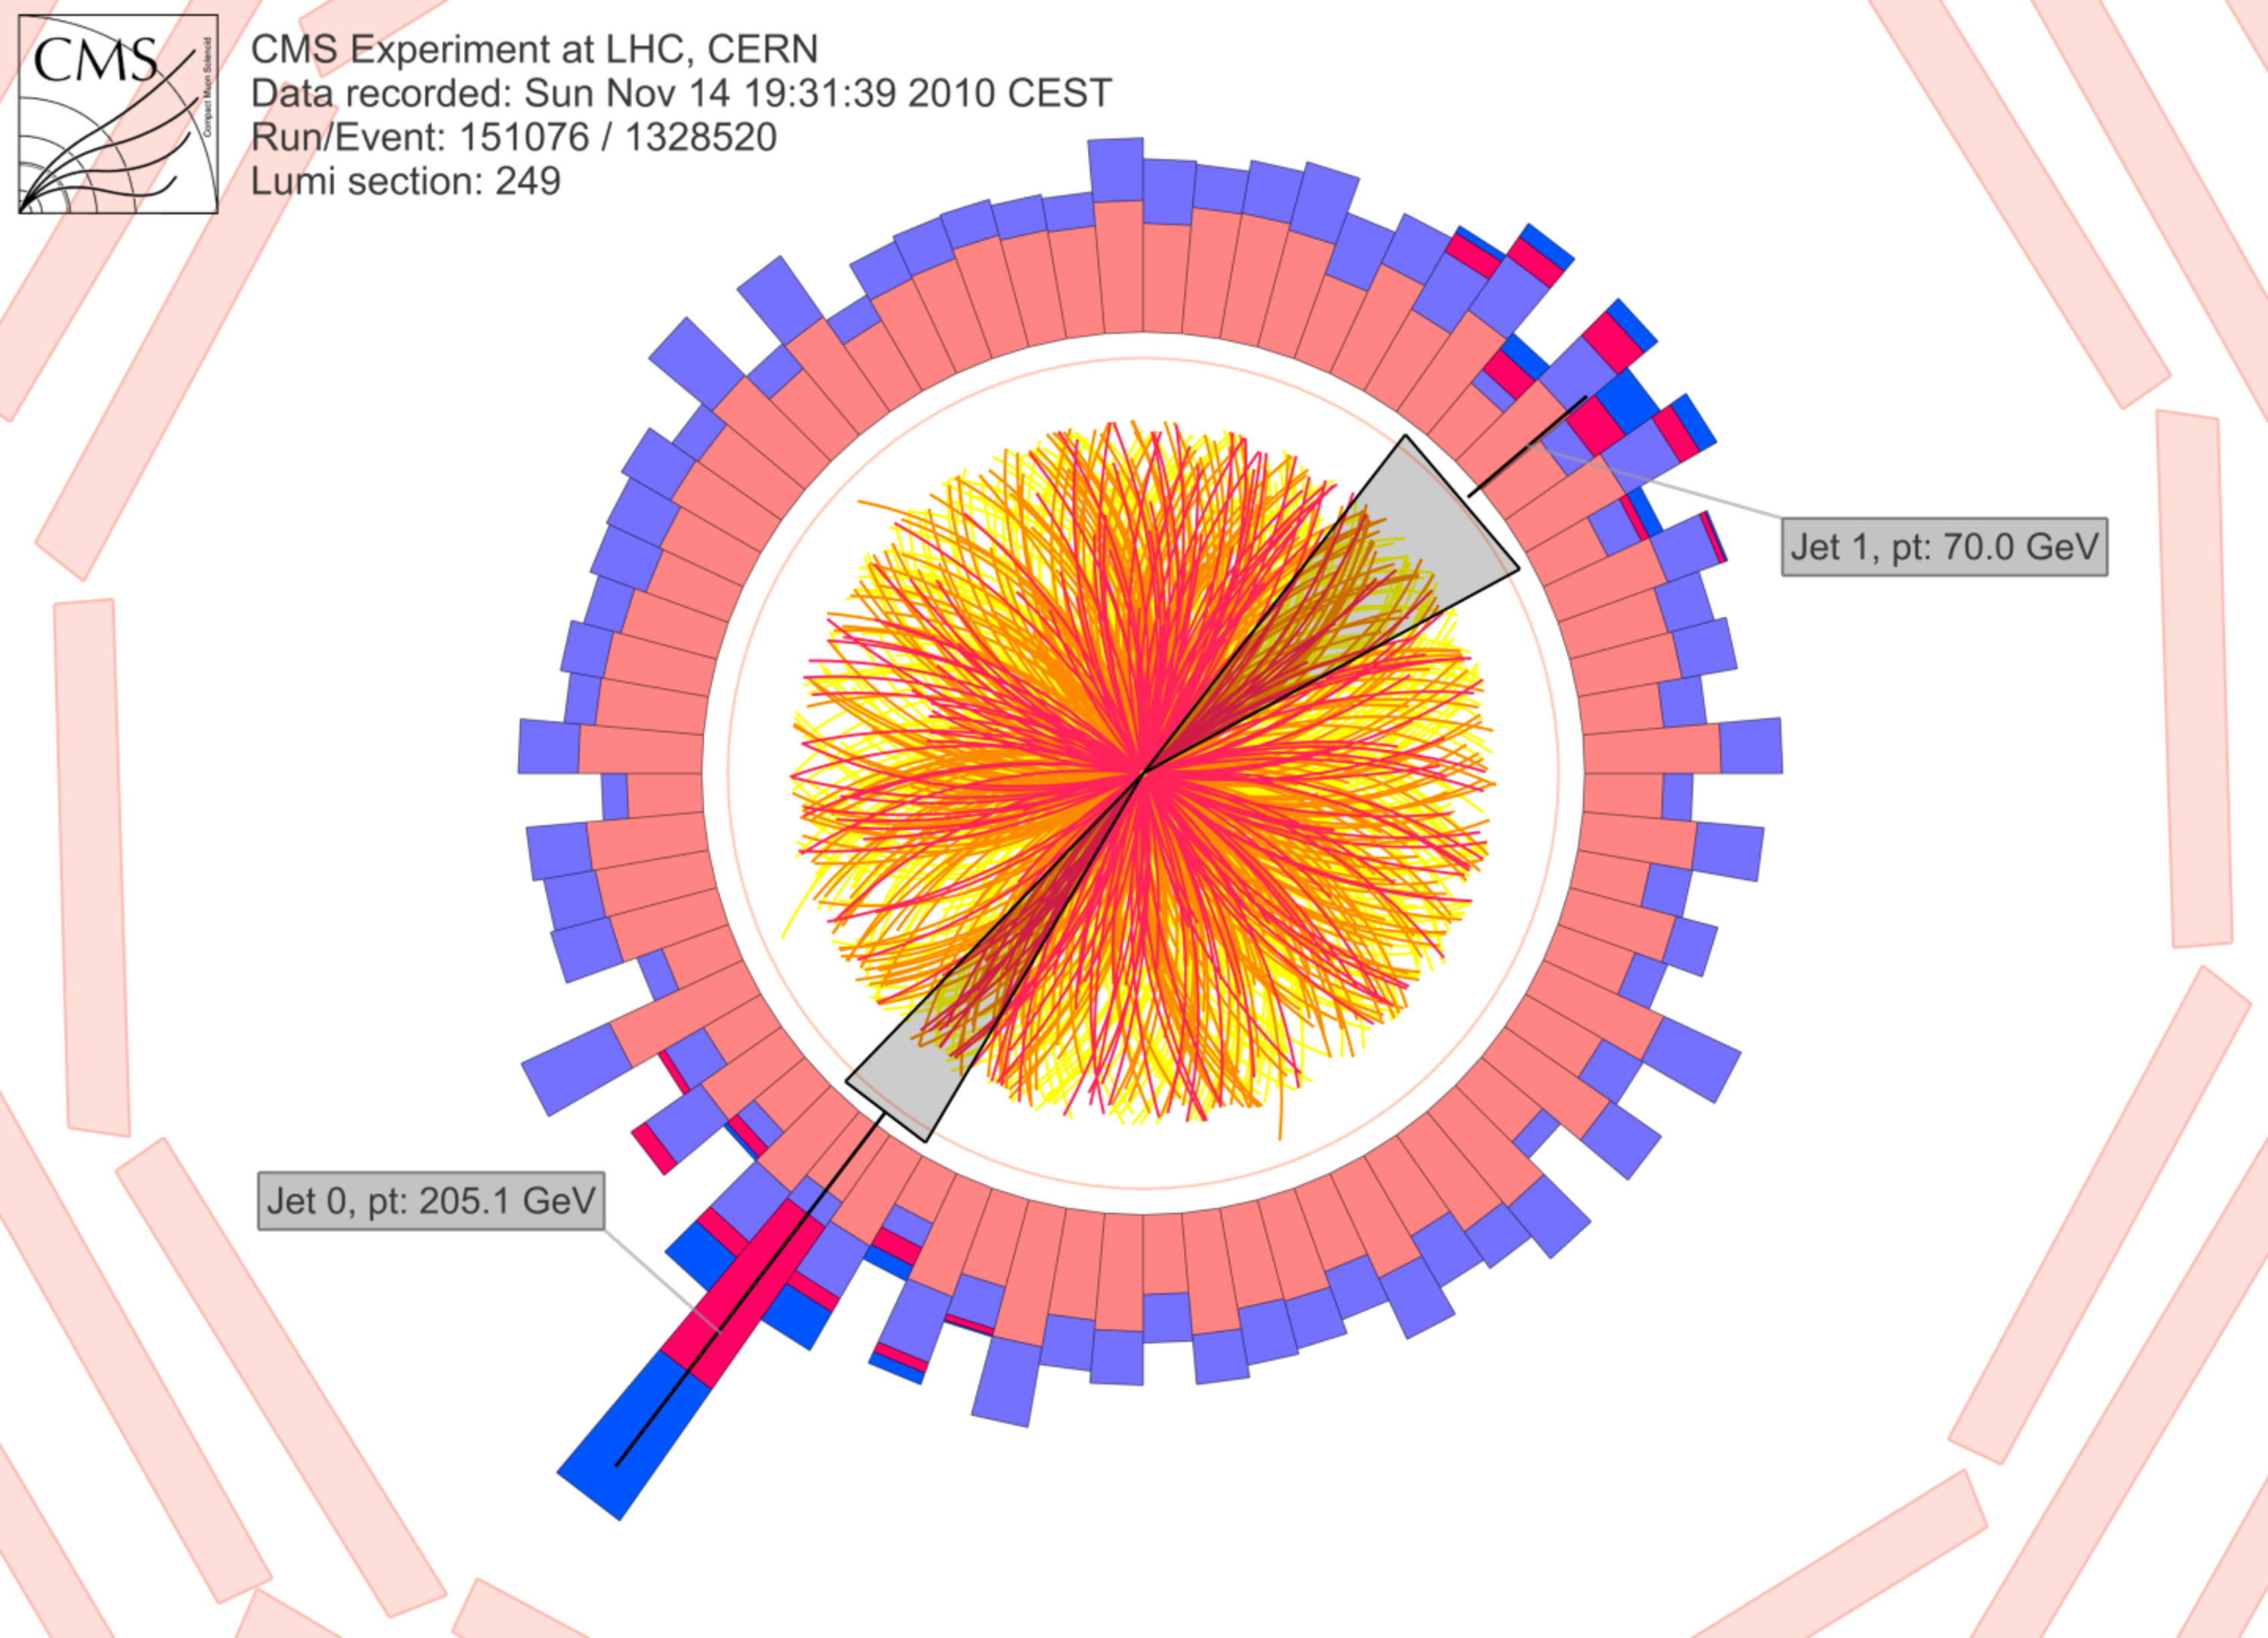
\includegraphics[height=11em]{\imgpath/DijetAA.pdf}}
\caption{Event displays from CMS in azimuthal plane showing a collision of \textbf{(a)} pp and \textbf{(b)} Pb-Pb with a dijet. The red and blue columns correspond to energy deposits in the detector calorimeters. \cite{cmsCMSCollisionEvents2010, niidaSignaturesQGPRHIC2021}}
\label{fig:colls:jetquenching}
\end{figure}

\subsection{Cold nuclear matter effects}

It should be noted that apart from the QGP, other effects come into play due to the fact that the collision involves two nuclei instead of two protons. These effects are important caveats to bear in mind and include:

\begin{enumerate}
\item Nuclear (anti-)shadowing: Reflects the modification in production due to differences in nPDFs and PDFs. \cite{vogtShadowingEffectsPsi2015}
\item Cronin effect: Describes the initial parton energy loss due to scatterings in the nuclear medium and broadens measured \pt spectra. \cite{croninProductionHadronsLarge1975}
\item Nuclear absorption: Describes the dissociation of particles due to their interactions with the passing-by nuclear remnants \cite{wongIntroductionHighenergyHeavyion1990}. It is generally negligible at LHC energies.
\item Co-mover absorption: This is the effect of inelastic interactions with the hadron gas. \cite{ferreiroExcitedCharmoniumSuppression2015}
\end{enumerate}

These effects can be isolated and quantified in pA or very peripheral AA collisions.

\section{QGP phenomena in small systems}\label{sec:colls:qgpss}

Measurements within the last decade have shown that certain QGP phenomena can also be observed in high-multiplicity events of pp collisions at LHC energies, which challenges the traditional assumption that QGP is only produced in AA collisions. This has sparked debates about the existence of QGP in pp collisions and, to a lesser degree, about the absence of QGP in AA collisions, despite the extensive experimental evidence.

Furthermore, the observed behavior of these phenomena indicates that the role of event multiplicity \Nch may be more significant than the collision system size. This has led to ongoing efforts to establish a consistent and seamless link between the paradigms of pp and AA collisions.

\subsubsection*{Strangeness and charm enhancement}

ALICE measurements on $\LA/\pi$, $\XI/\pi$, and $\Omega/\pi$ ratios demonstrate that the production rates of particles containing strange quarks increase faster with multiplicity than those containing only u and d quarks \cite{adamEnhancedProductionMultistrange2017}. This also depends on the strangeness content -- the effect is the strongest for $\Omega$ and vanishes for protons. Furthermore, the evolution to larger systems seems to be continuous with respect to \Nch. The measurements can be seen in Fig.~\ref{fig:colls:ssstrangeness} \cite{alicecollaborationALICEExperimentJourney2022}.

To contrast the strangeness measurements with charm, the $J/\psi \ /\pi$ ratio also shows a clear increase in yield with increasing \Nch in pp collisions, as is shown in Fig.~\ref{fig:colls:ssstrangeness} \cite{alicecollaborationMultiplicityDependencePsi2020, alicecollaborationObservationMultiplicityDependence2022}. However, this comes with an important caveat: high-multiplicity events are biased to have enhanced hard processes, as discussed further in Chapter~\ref{chap:rt}. Moreover, the evolution of this phenomenon is also not continuous with \Nch when going from pp collisions at \sppt{13} to \snnt{5.02}, which can also be explained by the fact that charm quarks are produced solely in hard scattering processes, the rates of which depend on the collision system and center-of-mass energy.

\begin{figure}[H]
\subfloat[][]{\adjincludegraphics[trim={0 0 {.48\width} 0},clip,height=15em]{\imgpath/ss_strangeness1.pdf}}\hspace{2em}
\subfloat[][]{\adjincludegraphics[trim={0 0 {.948\width} 0},clip,height=15em]{\imgpath/ss_strangeness2.pdf}\adjincludegraphics[trim={{.52\width} 0 0 0},clip,height=15em]{\imgpath/ss_strangeness2.pdf}} 
\caption{Ratios of integrated yields of \textbf{(a)} various light-flavour hadrons \cite{adamEnhancedProductionMultistrange2017} and \textbf{(b)} charm mesons \cite{alicecollaborationMultiplicityDependencePsi2020, alicecollaborationObservationMultiplicityDependence2022} to pions as a function of multiplicity in pp, p-Pb, and Pb-Pb collisions. \cite{alicecollaborationALICEExperimentJourney2022}}
\label{fig:colls:ssstrangeness}
\end{figure}

\subsubsection*{Anisotropic flow}

Azimuthal correlations and anisotropic flow measurements in small collision systems exhibit features similar to those observed in AA collisions, hinting at the presence of collective expansion \cite{cmscollaborationEvidenceCollectivityPp2017}. However, in small systems, these measurements are particularly challenging due to their large sensitivity to non-flow effects, such as jet fragmentation or resonance decays, which can mimic the features of collective flow. 

While models using hydrodynamic-like descriptions seem to be able to describe $v_2$ results (despite the fact that their assumption $\lambda \ll L$ is not valid) \cite{wellerOneFluidRule2017}, especially at high multiplicities, the interpretation of the results in small systems is still under investigation. The values of elliptic flow $v_2$ seem to be comparable to those in low-multiplicity Pb-Pb collisions, although the evolution of $v_2$ across different system sizes does not appear to be smooth. The measurements from CMS displaying a clear ridge in high-multiplicity events \cite{cmscollaborationEvidenceCollectivityPp2017} and the $v_2$ results from ALICE \cite{alicecollaborationInvestigationsAnisotropicFlow2019} can be seen in Fig.~\ref{fig:colls:ssv2}.

\begin{figure}[H]
\subfloat[][]{\adjincludegraphics[trim={0 {0.67\height} 0 0},clip,width=0.45\textwidth]{\imgpath/ss_ridge1.pdf}}
\subfloat[][]{\adjincludegraphics[trim={0 {0.67\height} 0 0},clip,width=0.45\textwidth]{\imgpath/ss_ridge2.pdf}}\\
\adjincludegraphics[trim={0 {0.7\height} 0 0},clip,width=0.8\textwidth]{\imgpath/ss_v2.pdf}
\subfloat[][]{\adjincludegraphics[trim={0 0 0 {0.966\height}},clip,width=0.8\textwidth]{\imgpath/ss_v2.pdf}}
\caption{\textbf{(a, b)} Two-dimensional two-particle correlation functions of charged hadrons in low (left) and high (right) multiplicity events of pp collisions at \sppt{13}. \cite{cmscollaborationEvidenceCollectivityPp2017} \textbf{(c)} Elliptic flow measured using two-particle cumulants with a pseudorapidity separation in pp, p-Pb, Xe-Xe, and Pb-Pb collisions as a function of multiplicity. \cite{alicecollaborationInvestigationsAnisotropicFlow2019}}
\label{fig:colls:ssv2}
\end{figure}

\subsubsection*{Radial flow}

Measurements of the ratio of \LA to \KOs \pt spectra ratio were also studied in pp collisions with differing \Nch, see Fig.~\ref{fig:colls:ssrflow} \cite{alicecollaborationMultiplicityDependenceMulti2020}. The boost of a collectively expanding system, as expected in the context of radial flow, should have a greater impact on heavier hadrons, leading to an enhancement of the baryon-to-meson ratio at intermediate \pt. This enhancement is observed in the \LA/\KOs ratio, its magnitude increases with increasing \Nch and the peak position shifts towards higher values collisions, consistent with the hydrodynamic picture. The increase at intermediate momenta leads to a corresponding depletion at low \pt. High-\pt (as well as integrated) \LA/\KOs ratios exhibit essentially no (or minor) multiplicity dependence. This observation also applies to proton-to-pion ratios. 

Recent studies have also investigated the charmed baryon-to-meson ratio $\LA_c/\mathrm{D^0}$, with similar findings, although measurements with smaller uncertainties are still required. Fig.~\ref{fig:colls:ssrflow} presents the corresponding results.

\begin{figure}[H]
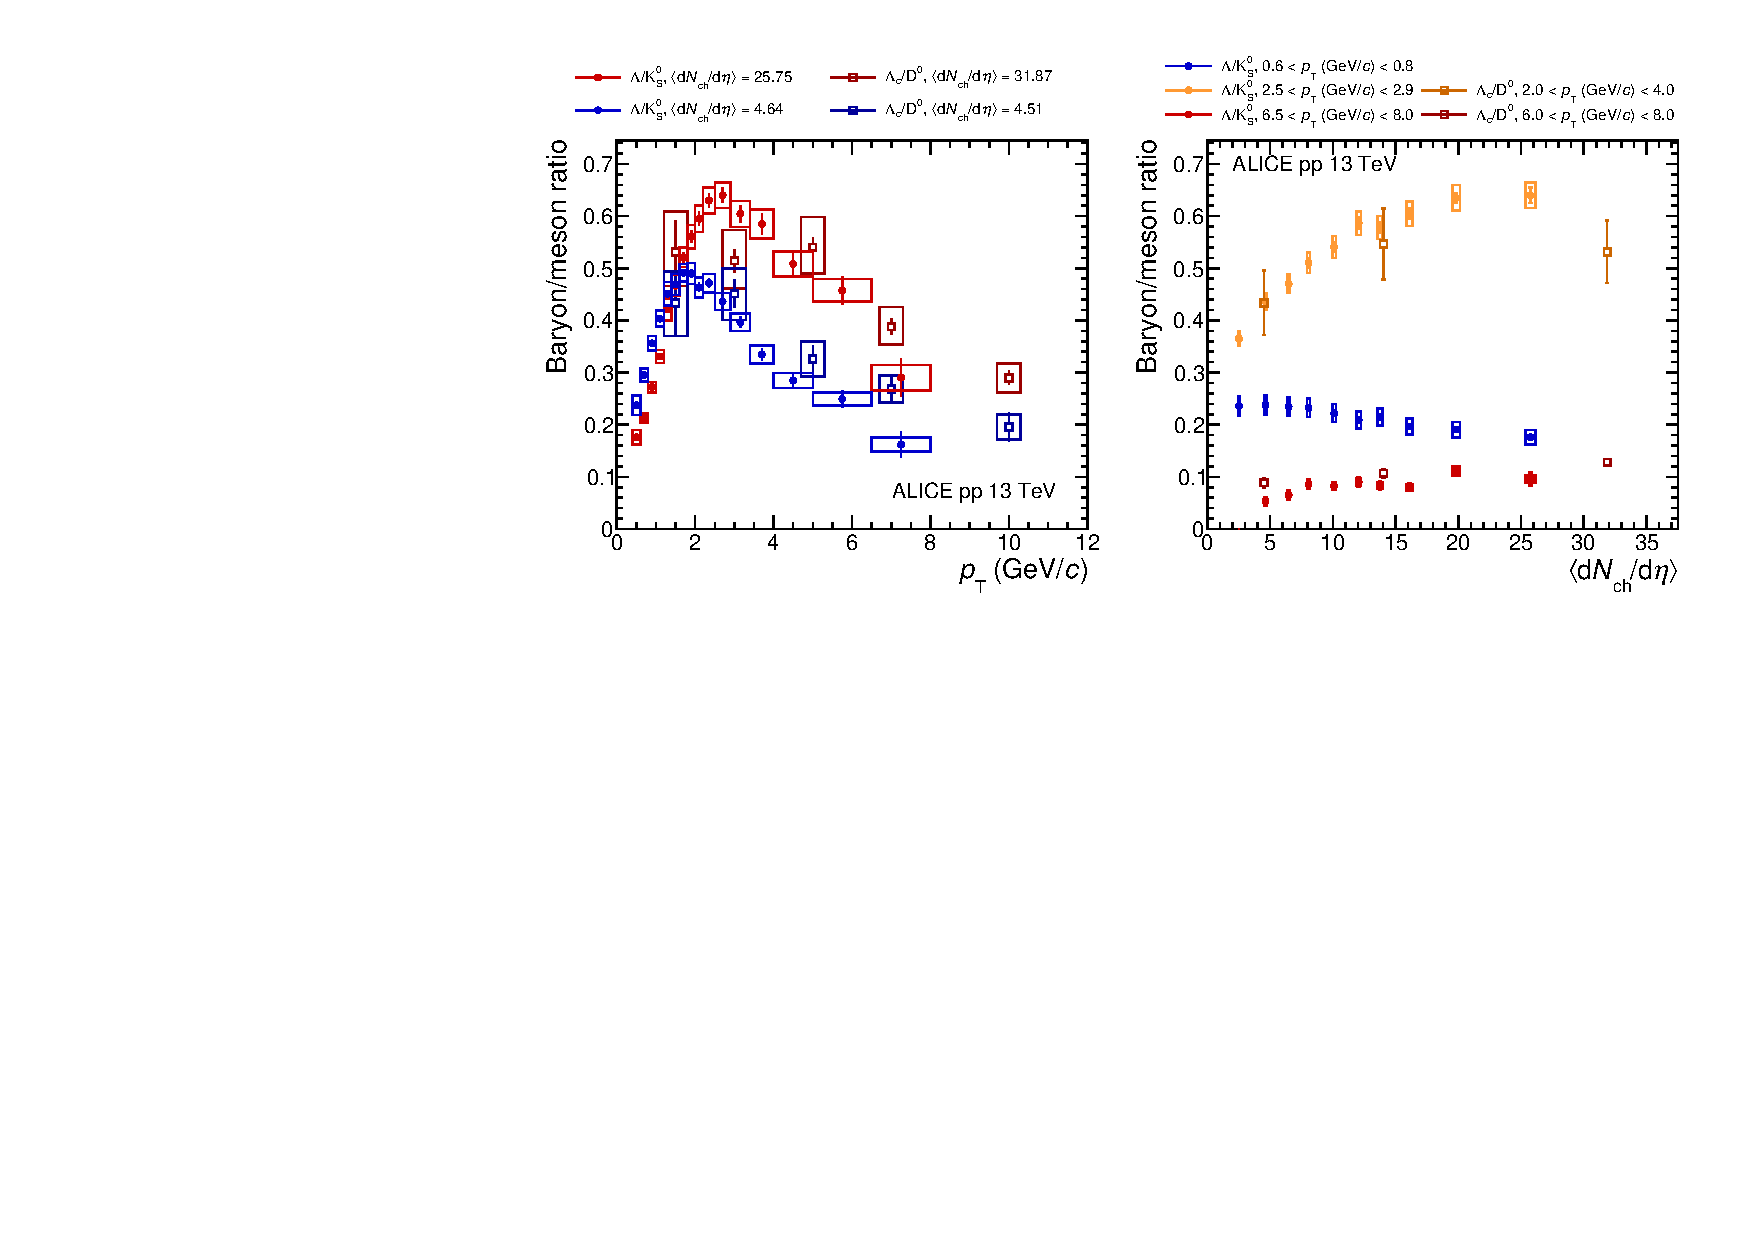
\includegraphics[width=.90\textwidth]{\imgpath/ss_rflow.pdf}
\caption{Baryon-to-meson ratios shown as the \pt differentials (left) and integrated yields in various \pt ranges as a function of multiplicity (right) for the \LA/\KOs and $\LA_c$/$\mathrm{D^0}$ in pp collisions at \sppt{13}. \cite{alicecollaborationMultiplicityDependenceMulti2020, alicecollaborationObservationMultiplicityDependence2022, alicecollaborationALICEExperimentJourney2022}}
\label{fig:colls:ssrflow}
\end{figure}

\subsubsection*{Sequential suppression of $\Upsilon$ states}

While defining $R_\mathrm{AA}$ to compare high-multiplicity and low-multiplicity events is unclear, and measuring yields as a function of \Nch is complicated by its biases related to the hardness of primary scatterings, it is worthwhile to investigate the ratio of excited-to-ground states of quarkonia as a function of \Nch.

Interestingly, these results \cite{cmscollaborationInvestigationEventactivityDependence2020} exhibit a decrease with increasing \Nch, resembling the pattern of sequential suppression due to QGP deconfinement. Even more remarkable, this dependence disappears in low-sphericity, jet-dominated, events (event shape observables such as sphericity are discussed in more detail in Chapter~\ref{chap:sphero}). These findings, reported in Fig.~\ref{fig:colls:ssupsilon}, suggest that the dependence on \Nch is solely influenced by the UE, rather than jets. As event multiplicity grows larger, excited $\Upsilon$ states become relatively less likely to be measured compared to the ground state.

These results indicate the need for a better understanding of $\Upsilon$ hadronization and the role UE may play in it. They also raise the question of whether the ground state is enhanced rather than the excited states being suppressed. Additionally, the effects of the mass differences must also be considered. However, the fact that low-sphericity, jet-dominated events have the same ratios as high-sphericity, UE-dominated events at low \Nch argues against these ideas.

An important caveat to note is that hadronic decays (which are dominant) of the heavy $\Upsilon$ states may result in tens of produced particles \cite{behrendsInclusiveHadronProduction1985}. Therefore, even minor discrimination against the excited states could hypothetically be correlated with a substantial but trivial increase in the accompanying \Nch. To the author's knowledge, there are currently no available phenomenological descriptions of the observed behavior, which further limits potentially groundbreaking interpretations.

\begin{figure}[H]
\subfloat[][]{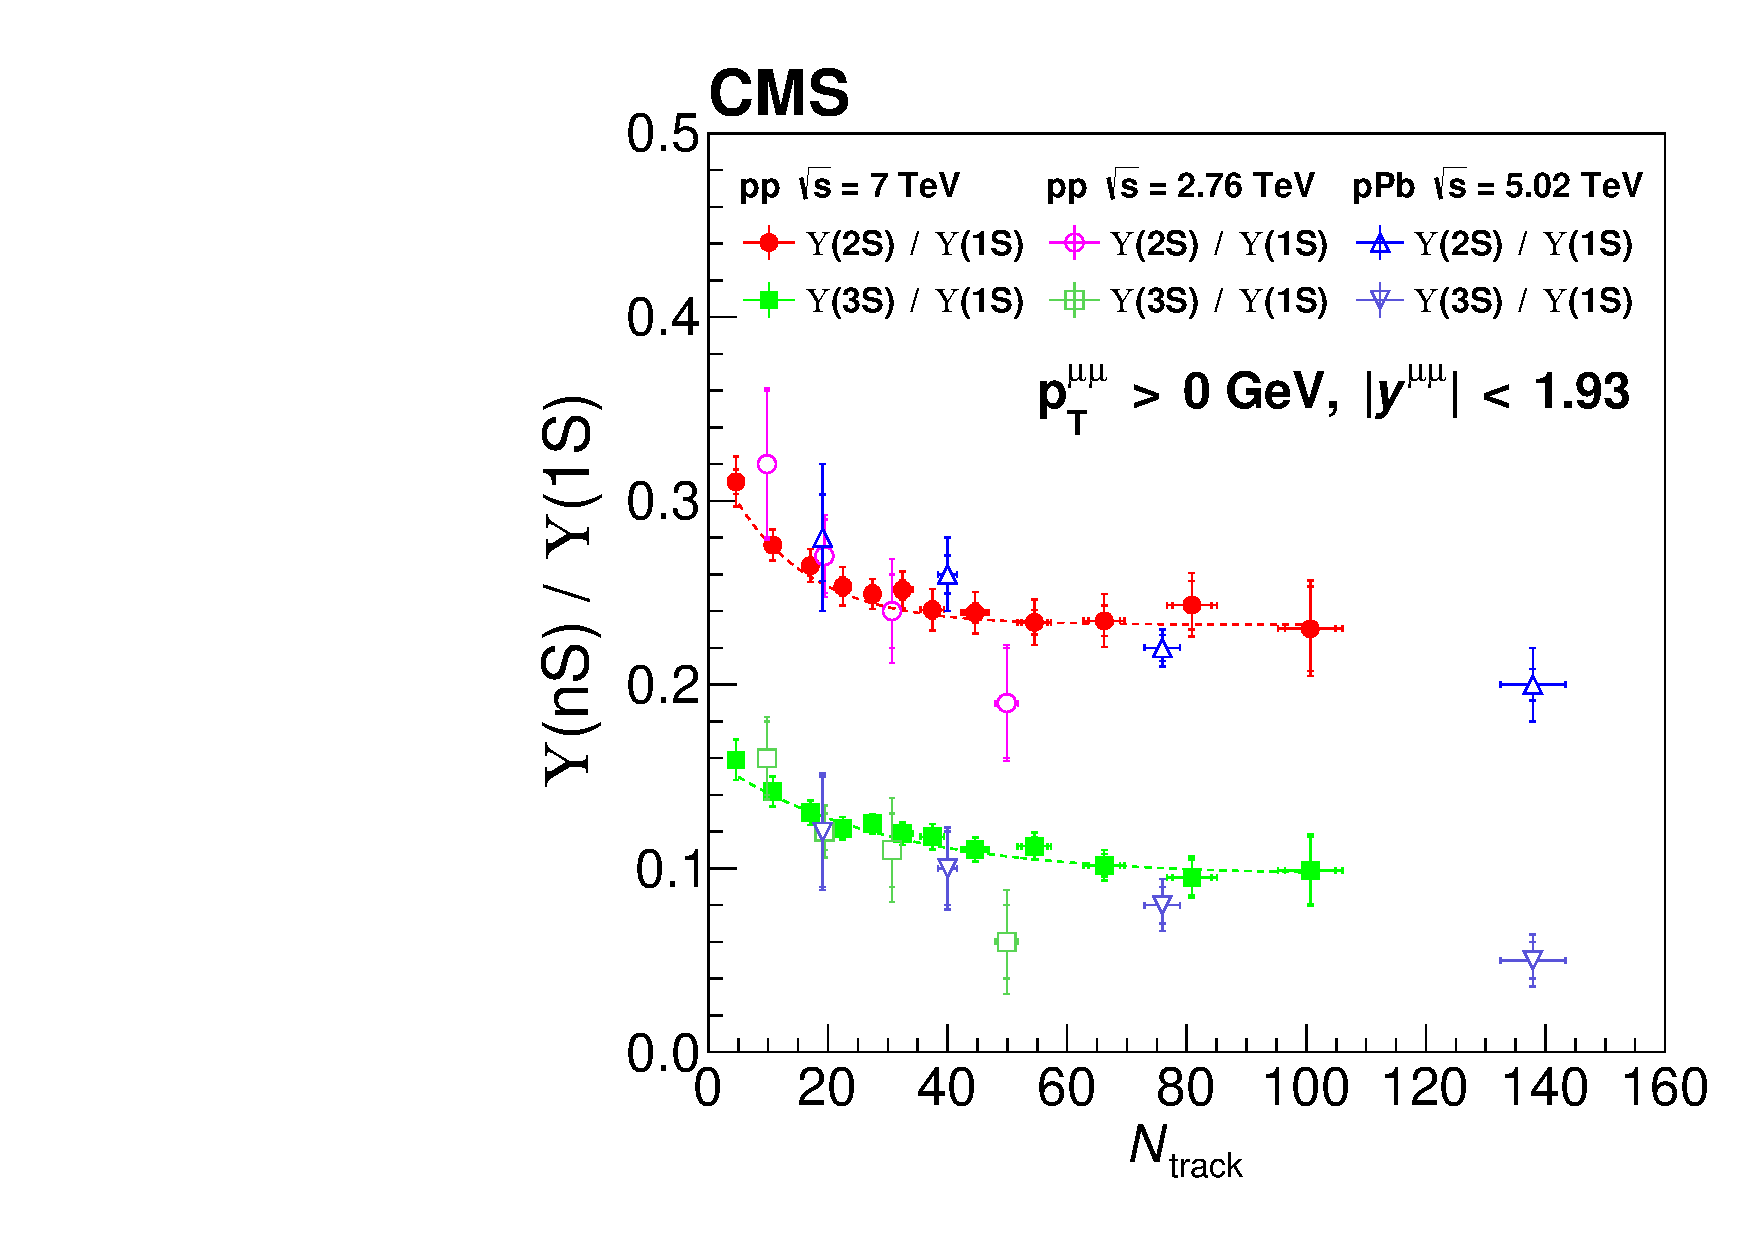
\includegraphics[width=.40\textwidth]{\imgpath/ss_ups1.pdf}}\hspace{1em} 
\subfloat[][]{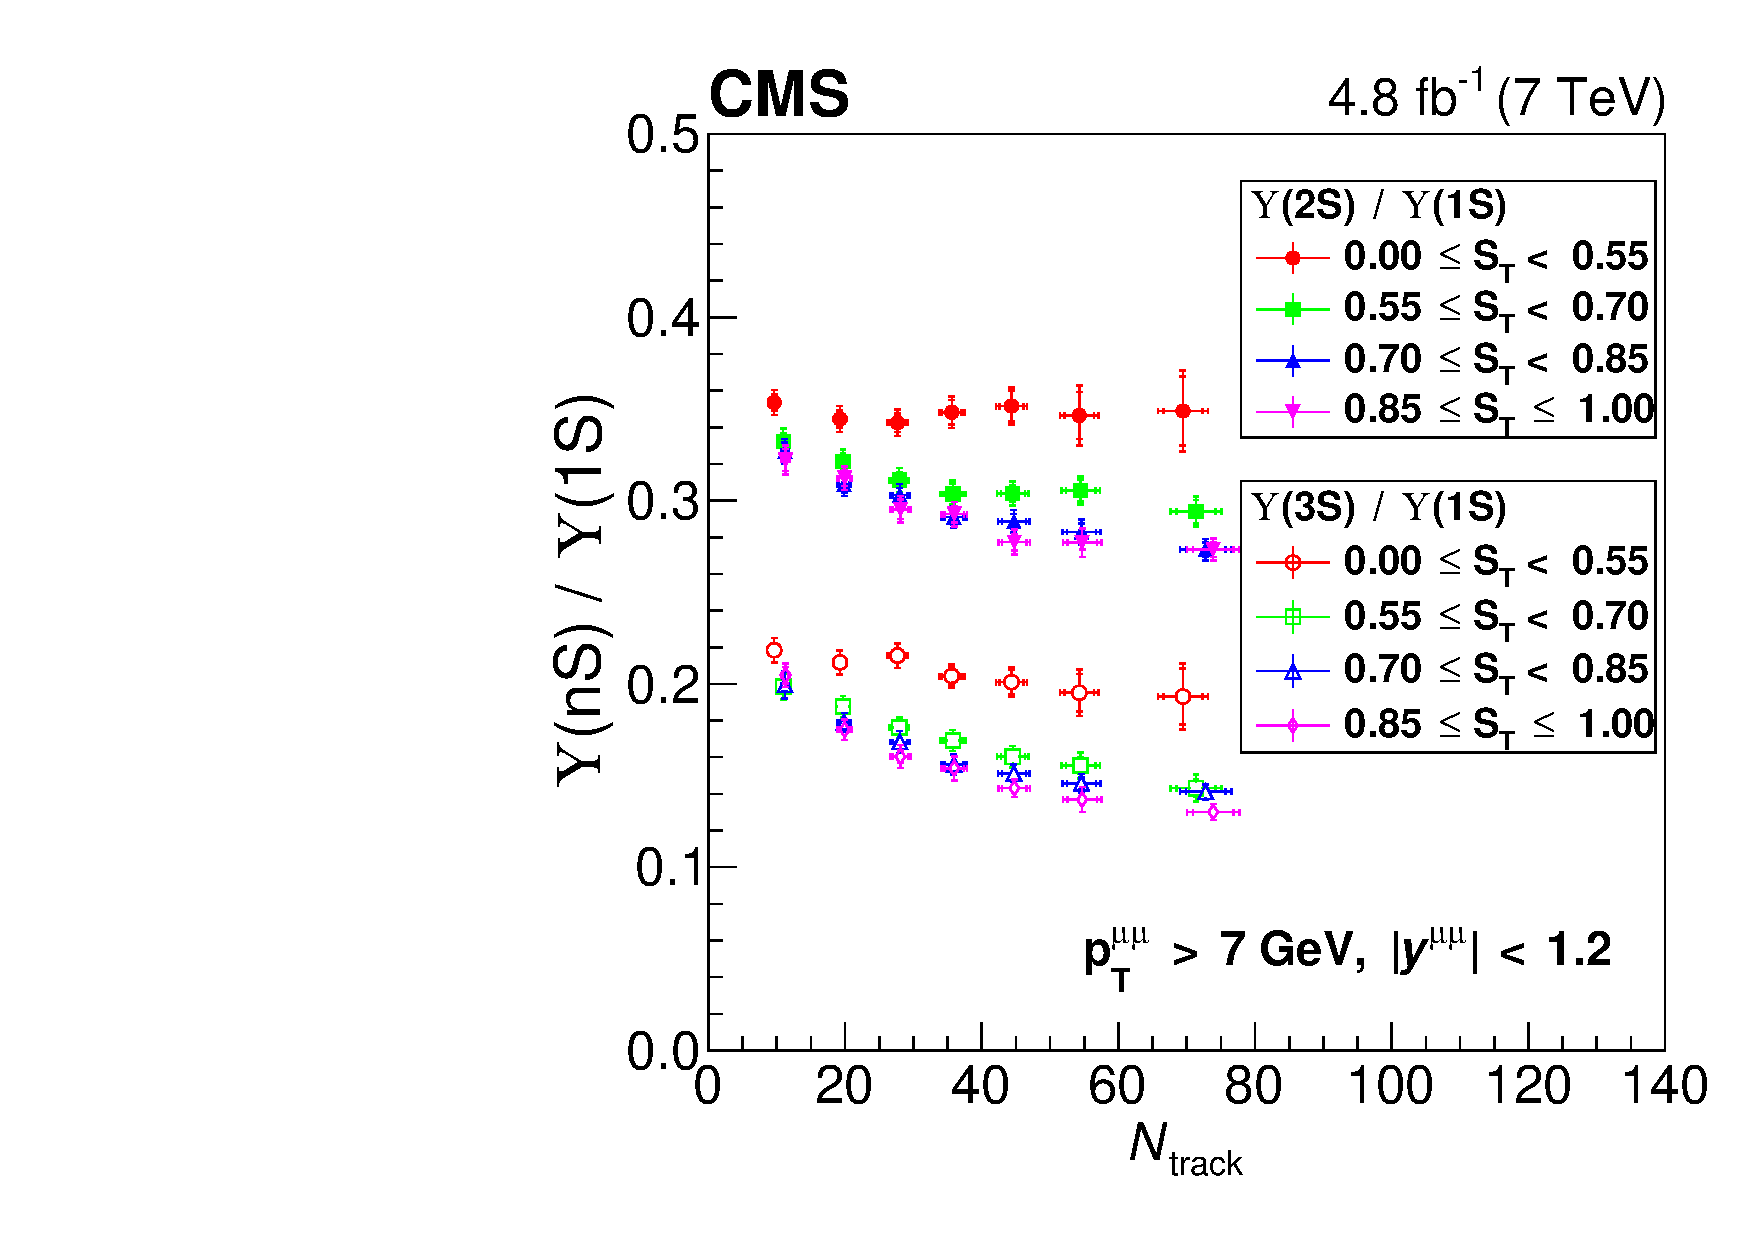
\includegraphics[width=.40\textwidth]{\imgpath/ss_ups2.pdf}}
\caption{The $\Upsilon$(2S)/$\Upsilon$(1S) and $\Upsilon$(3S)/$\Upsilon$(1S) ratios of measured yields in pp collisions as a function of \textbf{(a)} multiplicity, compared with p-Pb results, and \textbf{(b)} multiplicity and transverse sphericity, with the di-muon transverse momentum $\pt^{\mu\mu}>\gevc{7}$. \cite{cmscollaborationInvestigationEventactivityDependence2020}}
\label{fig:colls:ssupsilon}
\end{figure}

\subsubsection*{Other QGP signatures}

If a QGP is formed in small systems with sufficient volumes, the effect of jet quenching should be observed. One can also expect to observe it, due to the fact that in small systems, high-\pt hadrons have been measured to have finite flow $v_2$ \cite{cmscollaborationEllipticFlowCharm2018}, which could indicate that hard partons interact with an expanding medium. Whilst theoretical approaches do not provide unambiguous answers on whether this phenomenon can be observed \cite{zakharovPartonEnergyLoss2014} or not \cite{chenCentralityDependenceProductions2015}, experimental results on jet quenching in both pp and p-Pb collisions are consistent with no observable effect, within uncertainties \cite{alicecollaborationConstraintsJetQuenching2018}. These results are mostly based on measuring jet yields as a function of event activity, although such measurements are challenging due to fluctuations and interplays between jet characteristics and event activity.

\subsection{Role of multiplicity}

The observations made above highlight the significance of studying the role of multiplicity \Nch. In contrast to AA collisions, high-multiplicity events in pp collisions do not arise from a mere increase in the amount of colliding matter, as the values of \Npart and \Ncoll are fixed:
\begin{align}
\Npart = 2 \, ,\quad \ \Ncoll = 1 \, .
\end{align} 

Additionally, due to the relatively constant initial system volume, high-\Nch pp events may exhibit energy densities that exceed the threshold for QGP formation, given that the highest \Nch values are similar to those observed in peripheral AA collisions, where QGP formation is observed.

Clearly, the picture is more complex and despite its simplicity as an event activity classifier, \Nch poses challenges when it comes to relating data to theory since it cannot be directly linked to the initial state, and multiplicities in different events may originate from entirely different processes.

To address these issues and gain a better understanding of the evolution between low and high multiplicities and the potential for QGP formation, this dissertation focuses on transverse spherocity \SOPT and underlying event activity \RT measurements. The goal of these studies is to provide a deeper insight into the relevant degrees of freedom involved.

%One expects a trivial difference as the pT spectra are being measured at midrapidity in the same kinematic region where the midrapidity multiplicity selection is done. However, the slope of the pT spectra at high-pT indicates that the midrapidity estimator selects harder and harder subnucleonic interactions as the multiplicity increases. The ratios obtained with the forward estimator do not show a change in slope at high-pT. Still, the hard high-pT production is more enhanced than soft low-pT production in highmultiplicity collisions and vice versa in low-multiplicity collisions. This implies that the scaling with multiplicity of soft and hard processes is fundamentally different in pp compared to nucleus–nucleus collisions.

%a study with PYTHIA 8 (Monash 2013 tune) shows that the forward multiplicity estimator has the strongest correlation between the number of MPIs and the multiplicity. For this reason, the forward multiplicity slicing is used for multiplicity selection in the rest of this section unless specifically noted otherwise. As the multiplicity selection is done on charged particles, a second advantage of the forward selection is that it does not create an imbalance between charged and neutral particles at midrapidity

\section{Phenomenological models}

The next parts of this thesis give an overview to phenomenological models and event generators pertinent to the measurements in Chapters~\ref{chap:sphero} and \ref{chap:rt}. Other generators, such as Herwig 7 \cite{bellmHerwigReleaseNote2020} or Sherpa \cite{bothmannEventGenerationSherpa2019}, are not discussed here.

\subsection{Pythia}

Pythia is a Monte Carlo event generator used to simulate full events of high-energy particle collisions, based mostly on approximately perturbative QCD, with some important non-perturbative aspects. With more than four decades of development, only a brief overview is given in this thesis, whilst detailed description can be found in Ref.~\cite{bierlichComprehensiveGuidePhysics2022, sjostrandPYTHIAEventGenerator2020}. It has a modular structure to simulate different aspects of the collision process and includes the simulation of the initial kinematics, hard scattering, multiple parton interactions, parton showering, and hadronization, which were all discussed in Chapter~\ref{chap:intro}. The various components of the event simulation, such as the matrix element for the primary scattering, or even the parton evolution, can also be replaced with external alternatives. 

Its current and in ALICE most widely used version is Pythia 8, specifically its Monash tune \cite{skandsTuningPYTHIAMonash2014}, incorporating colour reconnections. Pythia has also included the implementation of Angantyr \cite{bierlichAngantyrModelHeavyIon2018}, a new model for the simulation of collisions of nuclei.

A pp collision event, as simulated by Pythia, can be seen in the illustration in Fig.~\ref{fig:colls:pythia} and crudely structured as:
\begin{enumerate}
\item Relevant parton kinematics are determined based on the PDFs of the beam particles and nature of the event is decided (e.g.\ $Z^0$ production). Produced resonances decay.
\item All subsequent partonic activity is simulated. This includes the initial- and final-state parton radiation, MPIs, and handling of the beam particle remnants. Eventually, after the full parton shower evolutions, a full partonic structure and string configuration is given.
\item Hadronisation occurs by the Lund string model fragmentation. This part is completely non-perturbative and fully phenomenological. Unstable particles decay and a full final-state particle collection is obtained. \cite{sjostrandBriefIntroductionPYTHIA2008}
\end{enumerate}

\begin{figure}[H]
\includegraphics[width=.90\textwidth]{\imgpath/pythia.pdf}
\caption{Diagram depicting a full simulation of pp collision event with its various components. For full description, see Ref.~\cite{bierlichComprehensiveGuidePhysics2022}.}
\label{fig:colls:pythia}
\end{figure}

\subsection{String interactions and Ropes}

While some effects typically associated with QGP formation, such as radial flow, can be somewhat mimicked in Pythia by colour reconnection \cite{bierlichEffectsColourReconnection2015, ortizColorReconnectionFlowlike2013}, as touched upon in Sec.~\ref{sec:intro:cr}, it is not sufficient to describe the strangeness enhancement patterns observed in small systems.

Ideas that overlapping QCD strings in high-density environments interact and form higher-tension ropes date back to modelling AA collisions in 1984 \cite{biroColourRopeModel1984} and have been explored further \cite{sorgeColourRopeFormation1992}, specifically in the framework of the DIPSY model \cite{bierlichEffectsOverlappingStrings2015}. This ``rope hadronisation" approach is also incorporated similarly in Pythia 8 and can be included in its simulations, which in the context of this dissertation will be referred to as the Pythia 8 Ropes tune.

In Pythia, strings are considered overlapping on purely geometrical considerations and utilise a parameter $\alpha$ to quantify the size of strings relatively to the proton radius. Combining two strings follows an algebra based on the SU($3$) group, described below, following a more detailed discussion in Ref.~\cite{bierlichEffectsOverlappingStrings2015}.

A $q\bar{q}$ string can be viewed as a SU($3$) triplet $\mathbf{3}$. Stacking another string suggests adding another triplet and forming a multiplet with quantum numbers $p$, corresponding to the number of coherent triplets $\mathbf{3}$ (e.g.\ all red), and $q$, corresponding to the number of coherent antitriplets $\mathbf{\bar{3}}$ (e.g.\ all anti-blue). Using a $\{p,q\}$ notation, the algebra for multiplets is as follows:
\begin{align}
\{1,0\} \otimes \{1,0\} = \{2,0\} \oplus \{0,1\} \quad ,\\
\{1,0\} \otimes \{0,1\} = \{1,1\} \oplus \{0,0\} \quad .
\end{align}

The first equation, physically, corresponds to merging of two colour strings with colour flows going in the same direction (same $q\bar{q}$ orientation), merging into a rope. When the colours are the same (e.g.\ both red), the result is a sextet rope $\mathbf{6}$, $\{2,0\}$. In other cases (e.g.\ red and blue), the result is an anti-triplet rope $\mathbf{\bar{3}}$, $\{0,1\}$ (corresponding to anti-green---green string). This algebra is illustrated in Fig.~\ref{fig:colls:ropes}.

The second equation describes stacking a triplet $\mathbf{3}$ with an anti-triplet $\mathbf{\bar{3}}$ (opposite colour flows and $q\bar{q}$ orientation). This results either in a gluon octet $\mathbf{8}$, $\{1,1\}$, or a singlet $\mathbf{1}$, $\{0,0\}$, with destructive interference and no colour flow.

The tension of the produced rope $\tilde{\kappa}$ is proportional to the quadratic Casimir operator $C_2$. When normalising to the tension of a single string $\kappa$, e.g.\ a $\{1,0\}$ triplet, the relative increase is given by
\begin{align}\label{eq:colls:string}
\frac{\tilde{\kappa}}{\kappa} = \frac{C_2( \{p,q\})}{C_2 ( \{1,0\})} = \frac{p^2+q^2+pq+3p+3q}{4} \quad ,
\end{align}
so in the example of adding two red triplets, the resulting $\{2,0\}$ rope tension is $\tilde{\kappa}=5/2$.

During hadronisation, the rope is assumed to break not entirely at once, but rather one string at a time. For the purpose of considering the probability of creating new quarks in (\ref{eq:intro:tunnel}), the effective tension from the $\{p,q\}\to \{p-1,q\}$ transition is given by (\ref{eq:colls:string}) and corresponds to
\begin{align}
\tilde{\kappa}_\mathrm{eff} = \frac{2p+q+2}{4}\kappa \quad.
\end{align}

This means that in the example of the $\{2,0\}$ rope breaking, the first quark creation comes with relative effective tension $\tilde{\kappa}_\mathrm{eff} = 3\kappa/2$, and the second one with the normal value of $\tilde{\kappa}_\mathrm{eff}=\kappa$.

The strangeness production suppression factor in (\ref{eq:intro:rho}) then becomes modified as
\begin{align}
\tilde{\rho} = \rho^{\frac{\kappa}{\tilde{\kappa}_\mathrm{eff}}} \quad ,
\end{align}
which makes it evident that overlapping many strings ($\tilde{\kappa}_\mathrm{eff} \to \infty$) results in $\tilde{\rho} \to 1$ and strange quarks are produced at the same rate as up and down. 

Furthermore, ideas for further interactions between strings, such as ``string shoving", wherein overlapping strings may repel each other due to transverse pressure from their excess energy, have also been developed. Such mechanisms produce effects similar to a hydrodynamically expanding medium, e.g.\ long-range anisotropic flow. \cite{bierlichShovingModelCollectivity2016}

\begin{figure}[H]
\subfloat[][]{\adjustbox{valign=m}{\includegraphics[width=.3\textwidth]{\imgpath/ropes1.png}}}\hspace{1em}
\subfloat[][]{\adjustbox{valign=m}{\includegraphics[width=.3\textwidth]{\imgpath/ropes2.png}}}\hspace{1em}
\subfloat[][]{\adjustbox{valign=m}{\includegraphics[width=.3\textwidth]{\imgpath/ropes3.png}}}
\caption{\textbf{(a)} Illustration of stacking two colour flow strings, triplets with colours $c_1$ and $c_2$.  \textbf{(b)} Rope sextet resulting from adding two coherent triplets, $c_1 = c_2$, $\{2,0\}$. \textbf{(c)} Resulting rope anti-triplet coming from adding two incoherent triplets, $c_1 \neq c2$, $\{0,1\}$. Illustrations are by C.\ Bierlich.}
\label{fig:colls:ropes}
\end{figure}


\subsection{EPOS LHC}

EPOS is an event generator built on the Gribov-Regge theory \cite{drescherPartonBasedGribovReggeTheory2001}, wherein several partons undergo multiple scatterings, each consisting of the hard scattering component as well as initial and final state linear parton emission. Together, they form a so-called parton ladder and correspond to a ``cut" pomeron exchange \cite{wernerPartonLadderSplitting2006}. The parton ladder represents a (mostly) longitudinally flowing colour field, a ``flux tube", which may hadronise via pair production.

To model the full collision process, EPOS combines a two-component core-corona approach. When the density of flux tubes in a given volume exceeds a parameter $\rho_0$, the core is formed. Conversely, flux tubes escaping the volume (usually with higher \pt) make up the corona. The core is assumed to evolve hydrodynamically, corresponding to a QGP droplet, and then hadronises collectively, where smaller core segments form hadrons following a statistical ensemble. Since the relative amount of core- and corona-related particle production can vary continuously, EPOS models can be used to describe pp, pA, and AA collisions using a single paradigm. \cite{pierogEPOSLHCTest2015}

EPOS models have been successful particularly at modelling soft-QCD physics and, apart from collider physics, are also widely used in studies of cosmic rays \cite{pierogEPOSModelUltra2009}. Throughout this dissertation, an adaptation of EPOS called EPOS LHC \cite{pierogEPOSLHCTest2015} is mostly used and shown, which only parametrises the flow dynamics of the core instead of implementing a full hydrodynamic simulation. Diagrams illustrating the partonic structure and core-corona mixing can be seen in Fig.~\ref{fig:colls:epos}.

\begin{figure}[H]
\subfloat[][]{\adjustbox{valign=m}{\includegraphics[width=.49\textwidth]{\imgpath/flux.eps}}}
\subfloat[][]{\adjustbox{valign=m}{\includegraphics[width=.39\textwidth]{\imgpath/core1.pdf}}}\\
\subfloat[][]{\adjustbox{valign=m}{\includegraphics[width=.39\textwidth]{\imgpath/coco_ratio.pdf}}}
\caption{\textbf{(a)} Illustration of the partonic structure in the form of a parton ladder. \cite{pierogEPOSLHCTest2015} \textbf{(b)} Visualisation of the core (red) and corona (green) components in a peripheral $20-40\%$ collision of Pb-Pb with 345 initial multiple scatterings, modelled by EPOS3 \cite{knospeHadronicResonanceProduction2016} \textbf{(c)} Fractions of particle production associated with the core (red) and corona (blue) regions in p-Pb and Pb-Pb collisions, modelled by EPOS3. \cite{knospeHadronicResonanceProduction2021}}
\label{fig:colls:epos}
\end{figure}

\part{Experimental Setup and Methodology}
\chapter{ALICE's adventures at the LHC}
%\def \imgpath {"./figures/alice"}


\begin{figure}%[!h]
\centering%
\includegraphics[width=.7\textwidth]{\imgpath/alicephoto.jpg}
\caption{TBA.}
\label{fig:experiment:cern}
\end{figure}

The ALICE (A Large Ion Collider Experiment) is one of four major detectors located at the Large Hadron Collider (LHC) at CERN. The ALICE detector is designed to study the properties of the quark-gluon plasma (QGP), a state of matter that existed a few microseconds after the Big Bang.

The ALICE detector consists of several sub-detectors that work together to capture and analyze the particles produced by the collisions at the LHC. The central component of the ALICE detector is the Time Projection Chamber (TPC), a large cylinder filled with a gas mixture that is used to detect the charged particles produced by the collisions. The TPC measures the position, momentum, and energy of the particles, allowing scientists to reconstruct their trajectories and identify the different particle species.

In addition to the TPC, the ALICE detector also includes several other sub-detectors, such as the Inner Tracking System (ITS), the Transition Radiation Detector (TRD), and the Time-Of-Flight (TOF) detector. The ITS is a high-precision tracking detector that is used to measure the trajectories of charged particles produced in the collisions. The TRD is used to identify electrons and measure their energy. The TOF detector measures the time-of-flight of particles and is used to determine their momentum.

\begin{figure}%[!h]
\centering%
\includegraphics[width=.7\textwidth]{\imgpath/alicescheme2.png}
\caption{TBA.}
\label{fig:experiment:cern}
\end{figure}


\begin{figure}%[!h]
\centering%
\includegraphics[width=.7\textwidth]{\imgpath/aliceevent.png}
\caption{TBA.}
\label{fig:experiment:cern}
\end{figure}

\section{Time Projection Chamber}

The TPC works by filling the cylinder with a gas, typically a mixture of helium and carbon dioxide, and applying an electric field to create a uniform drift velocity for the charged particles. As the particles move through the gas, they ionize the atoms, creating free electrons and ions. The electrons are then attracted to a central anode, where they are detected and used to reconstruct the particle tracks.

The TPC has a number of advantages over other types of detectors. For one, it is able to provide precise measurements of the position and momentum of the charged particles, which allows scientists to study the behavior of quark-gluon plasma and other forms of matter at extremely high temperatures and densities. The TPC is also able to reconstruct the tracks of thousands of particles produced in a single collision, which provides a comprehensive view of the event.

The TPC in the ALICE experiment is particularly advanced, with over 500,000 readout channels and a sensitive volume of over 90 cubic meters. It is able to operate at high collision rates, with a maximum readout rate of 50 kHz. The TPC also has a number of innovative features, such as a gating system that allows the detector to operate in the presence of large magnetic fields, and a continuous calibration system that ensures high data quality.


\begin{figure}%[!h]
\centering%
\includegraphics[width=.7\textwidth]{\imgpath/alicetpc.png}
\caption{TBA.}
\label{fig:experiment:cern}
\end{figure}


\section{Inner Tracking Systems}

The ITS is another tracking detector in the ALICE experiment, located closer to the collision point than the TPC. It is designed to provide precise measurements of the position of charged particles as they are produced in the collisions. The ITS consists of six layers of silicon detectors, which provide high-resolution measurements of the position and momentum of the particles. The ITS is particularly useful for studying the very early stages of the collision, where the particles are produced in a very small volume and with high energies.


\begin{figure}%[!h]
\centering%
\includegraphics[width=.7\textwidth]{\imgpath/aliceits.jpg}
\caption{TBA.}
\label{fig:experiment:cern}
\end{figure}

\chapter{Events, Tracks, and Vertices}
%\def \imgpath {"./figures/tracks"}

This Chapter provides an overview of the triggering and data preparation procedures at the ALICE experiment. The aim is to give the reader an understanding of the process of obtaining final objects representing the particles produced in hadronic inelastic collisions at the interaction point of the LHC, utilizing the experimental apparatus that was described in the previous chapter.

\section{Events and triggers}

The ALICE experiment uses a trigger system \cite{krivdaALICETriggerSystem2012, alicecollaborationPerformanceALICEExperiment2014} to accommodate the different detector read-out times, limited data storage, and to select interesting physics events from collisions with rates of roughly $8$~kHz for Pb-Pb collisions and up to $300$~kHz for pp collisions. The Central Trigger Processor (CTP) collects input data from the trigger detectors and makes a decision about whether to take or reject the event, with the trigger decision split into three levels: L0, L1, and L2. 

The L0 trigger level makes its decision based on the fastest detectors (e.g.\ the SPD and V$0$) and sends the decision back to detectors in $\sim 1.2$~$\mathrm{\mu s}$. The L1 trigger decision is based on all remaining fast detector inputs (also including e.g.\ the Zero Degree Calorimeters located $113$~m far from the IP) and arrives back into detectors in $6.5$~$\mathrm{\mu s}$. The final L2 trigger level waits for all the detector readouts, including the slowest TPC detector, happening in about $105$~$\mathrm{\mu s}$ time. Several trigger classes can be collected simultaneously during the data taking. Once an event passes the trigger decisions of the CTP, it is sent to the Data Acquisition System (DAQ) for more detailed processing and compression of the final data.

In ALICE measurements, the following names are commonly used for some of the triggered events:
\begin{itemize}
\item \spverb|kINT7| :  the usual minimum bias (MB) class in pp collisions, based on a coincidence of the \VOA and \VOC detectors,
\item \spverb|kINT1| : also a MB class, requiring at least two signals among \VOA, \VOC, and the SPD,
\item $|$\spverb|INEL>0|$|$ : requires a MB class and at least one SPD ``tracklet" within $|\eta|<1$, which is reconstructed in the two SPD layers.
\end{itemize} 

\section{Event and track reconstruction}

Reconstruction of the event information in the central barrel follows a procedure discussed in Ref.~\cite{} and summarised in Fig.~\ref{fig:tracks:flow}. It begins with clusterisation, where the detector data is transformed into clusters, or \textit{reconstruction points}, that include the spatial information, signal amplitude, signal time, and associated errors. The clusterisation is carried out locally for each detector, for instance, for the TPC, a cluster corresponds to a crossed row in the ROCs.  The next steps are discussed in this section.


--
Next, preliminary primary vertex (PV) is determined by utilising clusters in the first two ITS layers (SPD). The Kalman filter technique is employed to perform track finding and fitting in TPC and ITS. The discovered tracks are then matched to other detectors in the central barrel and fitted. The reconstructed tracks are used to determine the final interaction vertex. The central-barrel tracking procedure concludes with a search for photon conversions, strange hadron decays (K0
S/Λ, Ξ±, and Ω±), and V0 particles. The steps are discussed in greater detail in this section.

\begin{figure}%[!h]
\adjincludegraphics[trim={0 {.68\height} 0 {.07\height}},clip,width=.99\textwidth]{\imgpath/flow.pdf}
\caption{Work flow diagram of the event information reconstruction in the central barrel. \cite{LHCReportMake2023}}
\label{fig:tracks:flow}
\end{figure}

\subsection{First primary vertex determination}

A preliminary primary vertex (PV) is determined using tracklets formed in the two SPD layers of the ITS. A three-dimensional reconstruction is performed in pp and pA collisions, iteratively, so that events with in-bunch pile-up can be treated. With each iteration, clusters with tracklets already pointing to a vertex are removed. By construction, the first found vertex has the highest number of corresponding tracklets and is defined as primary. The If this method fails, the PV is determined only in the $z$-dimension. This is also the default in AA collisions. These methods are visualised in Fig.~\ref{fig:tracks:pvfirst}.

\begin{figure}%[!h]
\subfloat[][]{\includegraphics[width=.35\textwidth]{\imgpath/pv1.png}}\hspace{3em}
\subfloat[][]{\includegraphics[width=.35\textwidth]{\imgpath/pv2.png}}
\caption{\textbf{(a)} Preliminary three-dimensional reconstruction of the primary vertices, also depicting tracklets rejected by the algorithm. \textbf{(b)} Preliminary one-dimensional reconstruction of the PVs. \cite{alicedatapreparationgroupALICEDataFlow2018}}
\label{fig:tracks:pvfirst}
\end{figure}

\subsection{Tracking}

Track finding (recognition) and track fitting (reconstruction) is carried out simultaneously using the Kalman filter technique in three steps: inwards, outwards, inwards \cite{arslandokTrackReconstructionHighDensity2022}. The entire process is illustrated in Fig.~\ref{fig:tracks:tracking}. 

First, for \textit{primary} tracks, i.e.\ tracks hypothesised to originate from the PV, seeds are found from the preliminary SPD PV and pairs of TPC clusters at the highest radii, where track densities are the lowest. For \textit{secondary} tracks, coming for instance from weak decays with displaced secondary vertices, three TPC clusters are used instead of considering the PV. The track seeds are then projected inwards, adding clusters fulfilling given proximity cuts, and updating the track parameters at each step, until the inner TPC radius is reached. Preliminary $\mathrm{d}E/\mathrm{d}x$ is also stored. Moreover, tracks sharing multiple clusters (approx.\ more than $25\%$) are discarded in favour of their higher-quality doubles. 

The TPC tracks are then extrapolated to the ITS, where they continue to get updated. This tracking efficiency in the TPC, displayed in Fig.~\ref{fig:alice:pres}, drops significantly below $\approx \mevc{200}$, where energy loss and multiple scatterings start playing a role. For this reason, the ITS also runs a standalone Kalman filter algorithm, using clusters that are not associated with the TPC track. There, similarly to the TPC, candidates are considered both with and without a PV constraint.

In the second step, tracks are extrapolated to the point of closest approach (PCA) with respect to the PV and back-propagated to the TPC outer radius, using the previously added clusters. Now, track lengths are also considered and an expected time-of-flight (TOF) information is calculated based on the stored $\mathrm{d}E/\mathrm{d}x$. The tracks are then extrapolated to the Transition Radiation Detector (TRD), TOF, and possibly other detectors with clusters, where they can be matched with them. The ITS standalone tracks are propagated only to the ITS outer radius.

Finally, the tracks udpated with the TRD and TOF (and possible other) information are re-fitted in each detector inwards again, starting at the TPC outer radii and propagating to the PV PCA. As a result of using the Kalmar filter, the track parameters are then finalised and given unambiguously, at the point of the primary vertex. More than $90\%$ of the reconstructed tracks are primary tracks. This ratio can be significally enhanced by imposing transverse and longitudinal cuts on the distance of closest approach (DCA) to the PV.

\begin{figure}[!h]
\subfloat[][]{\adjustbox{valign=m}{\includegraphics[width=.38\textwidth]{\imgpath/first.png}}}\hspace{1em}
\subfloat[][]{\adjustbox{valign=m}{\includegraphics[width=.38\textwidth]{\imgpath/second.png}}}\\
\subfloat[][]{\adjustbox{valign=m}{\includegraphics[width=.38\textwidth]{\imgpath/third.png}}}
\caption{Diagrams illustrating the inward-outward-inward approach in central barrel tracking. \textbf{(a)} First: track seeding and propagation to ITS and PV. \textbf{(b)} Second: back-propagation through ITS and TPC and extrapolation to TRD and TOF. \textbf{(c)} Third: final re-fit. \cite{maireProductionBaryonsMultietranges2011}}
\label{fig:tracks:tracking}
\end{figure}

The ITS- and TPC-combined tracks enjoy the highest momentum resolution, which is plotted as a function of the track \pt in Fig.~\ref{fig:tracks:pres}. It corresponds to values of about $1\%$ at \gevc{1} and then continues increasing as higher-\pt tracks are less curved, thus less constrained, and more likely to have a larger part in the detector's inactive regions. The disadvantage of the ITS-TPC tracks is their azimuthal non-uniformity due to gaps in the ITS acceptance, particularly the SPD.

\subsubsection*{Final PV determination}

Subsequently, the ITS-TPC \textit{global} tracks are used to determine the PV with a higher precision than when using the SPD tracklets alone. Tracks are also weighted to minimise the effect of outliers and the nominal beam position can also be used as a space point. In high pile-up runs, an iterative vertex process is performed. Standard deviation of the vertex position in the transverse region ranges from $\sim 1$~mm in events with one track to $\sim 0.1$~mm in events with five tracks and more.

\begin{figure}[!h]
\subfloat[][]{\adjustbox{valign=m}{\includegraphics[width=.46\textwidth]{\imgpath/tpceff.eps}}}\hspace{1em}
\subfloat[][]{\adjustbox{valign=m}{\includegraphics[width=.40\textwidth]{\imgpath/reso.pdf}}}\\
\caption{\textbf{(a)} Efficiency of track finding in the TPC for primary particles in pp collisions (green) and Pb-Pb collisions at different centralities (blue and red), determined from simulations. \cite{alicecollaborationPerformanceALICEExperiment2014} \textbf{(b)} Transverse momentum resolution of the combined ITS-TPC tracking in Pb-Pb collisions. \cite{continPerformancePresentALICE2012}}
\label{fig:tracks:pres}
\end{figure}

\subsection{Finding secondary vertices}

After the track and primary vertex reconstruction, an algorithm is ran to find secondary vertices corresponding to photon pair conversions, the so-called \VOs (weak decays of e.g.\ the \KOs and \LA) and the so-called \textit{cascades} (\XI and $\Omega$),  based on the topology shown in Fig.~\ref{fig:tracks:topo}. First, pairs of unlike-signed tracks with a given DCA with respect to the PV are formed (more than $0.5$~mm in pp or $1.0$~mm in Pb-Pb). Furthermore, loose cuts on the topology of the decay (discussed in more detail in Chapter~\ref{chap:analysis}) are imposed. Specifically, 
\begin{enumerate}
\item the PCA of the two tracks with respect to each other needs to be closer to the PV than the inner-most cluster of either of them, which corresponds to the fact that the daughters are produced in the vertex,
\item the DCA of the two tracks needs to be smaller than $1.5$~cm,
\item if the two-track momentum exceeds $\pt>\gevc{1.5}$, cosine of the \textit{pointing angle} (CPA) between the formed momentum vector and the straight line connecting the two-track PCA and the PV needs to be larger than $0.9$.
\end{enumerate}

The \VOs search can occur ``online" during the tracking, using a full information of the clusters, or ``offline", at a later stage, where it is based on the reconstructed tracks and can be re-configured. Subsequently, a search for cascades is performed: the found secondary vertices are matched with other secondary \textit{bachelor} tracks if
\begin{enumerate}
\item the invariant mass of the found pair is consistent with that of a \LA, assuming a p and $\pi$ mass hypothesis for the two tracks,
\item the bachelor DCA to the PV exceeds $0.2$~cm.
\end{enumerate}

%Improved finder

\begin{figure}%
\includegraphics[width=.590\textwidth]{\imgpath/v0.eps}\\
\caption{Diagram showing topology of a \VO decay (in this case \KOs) and a cascade decay (in this case \XI) in the central barrel. Here, the decays occured within the ITS volume, but this is not a requirement for the reconstruction. The radii are not to scale. \cite{alicecollaborationPerformanceALICEExperiment2014}}
\label{fig:tracks:topo}
\end{figure}

\section{Centrality and multiplicity measurements and their caveats}

In Pb-Pb collisions, the experimentally measured multiplicity can be related to the centrality using the Glauber picture, as discussed in Chapter~\ref{chap:colls}, which maps the final state to the percentage of the total hadronic cross section based on the collision geometry. This picture assumes that the multiplicity due to the different \Npart dominates over contributions from specific event sub-structures (e.g.\ a hard jet), and that the effect of fluctuations is small enough to play a role. In ALICE, this procedure is performed typically using the \VOM estimator (as it has the highest centrality resolution \cite{alicecollaborationPerformanceALICEExperiment2014}). The \VOM is a summed amplitude in the two \VOA and \VOC forward-rapidity scintillators, and the mapping procedure is discussed in detail in e.g.\ Ref.~\cite{alicecollaborationCentralityDeterminationPbPb2013}.

Apart from the \VOM, multiplicity can also be estimated at mid-rapidity, using the SPD, which allows for taking into account particles with even very low momenta. This can be defined as either
\begin{itemize}
\item the number of clusters in the first layer of the SPD, also known as \spverb|CL1|,
\item or the number of formed tracklets in the SPD at $|\eta < 0.8$. This is also used in the studies done in this thesis and is referred to as \NSPD.
\end{itemize}

In pp collisions, the choice of mid-rapidity estimators comes with an important caveat when measuring particle spectra. Since event classification and tracking are performed in the same region, and fluctuations are not negligible compared to the multiplicities, an auto-correlation bias occurs. This can be seen in Fig.~\ref{fig:tracks:ktok}, which compares the integrated yields of charged kaons to neutral \KOs, scaled by a factor of two. As the multiplicity increases, the two yields become different, because requiring a large number of charged particles to classify the event as high multiplicity biases the charged kaon yields to higher values.

Furthermore, it should be noted that apart from this auto-correlation bias, spectra measured as a function of mid-rapidity and forward-rapidity multiplicity may still exhibit differences, as the choice of rapidity also plays a role when accessing and classifying the underlying dynamics of particle production in the event. This is illustrated in Fig.~\ref{fig:tracks:nmpi}, which shows a different dependence of the mean number of MPIs \meannmpi in Pythia 8 on the multiplicity selected by the two classifiers.

\begin{figure}[!h]
\subfloat[][]{\adjustbox{valign=m}{\includegraphics[width=.40\textwidth]{\imgpath/ktok_nch.pdf}}}\hspace{1em}
\subfloat[][]{\adjustbox{valign=m}{\includegraphics[width=.40\textwidth]{\imgpath/ktok_vom.pdf}}}\\
\caption{Dependence of charged and neutral kaon yields in pp collisions on the multiplicity determined \textbf{(a)} at mid-rapidity using the \NSPD estimator and \textbf{(b)} at forward rapidity using the \VOM estimator, as simulated by Pythia 8. \cite{alicecollaborationMultiplicityDependenceLightflavor2019}}
\label{fig:tracks:ktok}
\end{figure}

\begin{figure}[!h]
\subfloat[][]{\adjustbox{valign=m}{\includegraphics[width=.40\textwidth]{\imgpath/nmpi.pdf}}}
\caption{Mean number of MPIs as a function of multiplicity determined at mid-rapidity (black) and forward rapidity (red) in pp collisions at \sppt{13}, as simulated by Pythia 8. \cite{alicecollaborationALICEExperimentJourney2022}}
\label{fig:tracks:nmpi}
\end{figure}

\section{Used tracks}

The following tracks are often used in ALICE analyses and in the measurements within this dissertation:
\begin{itemize}
\item \spverb|ITSTPC2011|: The highest-quality ITS-TPC tracks, also referred to as ``global" tracks. They require TPC and ITS re-fit, TPC goodness-of-fit $\chi^2/n_\mathrm{cluster}^\mathrm{TPC} < 4$, ITS goodness-of-fit $\chi^2/n_\mathrm{cluster}^\mathrm{ITS} < 36$, $70$ crossed TPC rows, minimum $80\%$ of findable clusters based on geometrical considerations, clusters in the SPD, longitudinal DCA to the PV within $2$~cm, and no associated kink topology\footnote{In ALICE, decays of charged particles into one charged and one neutral daughter, e.g.\ $\pi^- \to \mu^- \bar{\nu_\mu}$, can be identified in the TPC from a characteristic ``kink" topology.}.
\item \spverb|TPCOnly|: Tracks with better azimuthal uniformity, which require TPC goodness-of-fit $\chi^2/n_\mathrm{cluster}^\mathrm{TPC} < 4$, $50$ crossed TPC rows, longitudinal DCA to the PV within $3.2$~cm, transverse DCA to the PV within $2.4$~cm, and no associated kink topology.
\item \spverb|V0daughter|: Secondary tracks used to find candidates for weakly-decaying \KOs and \LA (discussed further in Chapter~\ref{chap:analysis}), representing their charged daughters. They require a TPC re-fit, $70$ crossed TPC rows, and no kink topology.
\item Hybrid tracks: discussed below.
\end{itemize}

\subsection{Hybrid tracks}

For measurements requiring high track quality and momentum precision, such as for particle \pt spectra, the ITS-TPC tracks are usually used. As mentioned, these suffer from azimuthal non-uniformity due to the SPD acceptance. In situations where this is unacceptable, such as when using event shape observables or azimuthal topology classifications, ``hybrid tracks" can be used instead. These correspond to a union of ITS-TPC tracks and \textit{complementary tracks}, which are subjected to identical requirements save for the SPD cluster information. Furthermore, they must be constrained to the PV. A track can be classified as complementary only if it does not pass the ITS-TPC cuts first.

This union significantly improves the azimuthal uniformity, as displayed in Fig.~\ref{fig:tracks:hybrid}.

\begin{figure}%
\includegraphics[width=.790\textwidth]{\imgpath/InfoRT_tracks.pdf}\\
\caption{Azimuthal distributions of the standard ITS-TPC tracks (red), complementary tracks (blue), and their union: hybrid tracks (black), in events used for measurements presented in this thesis. }
\label{fig:tracks:hybrid}
\end{figure}

\subsection{Geometrical cuts on tracks}

In measurements using a high-momentum trigger particle, additional geometrical constraints can be utilised to ensure the low-curvature particle trajectory does not significantly cover an inactive sector of the TPC.

In order to have just one set of requirements independent of the magnetic polarity and the particle charge, the azimuthal $\phi' = \phi$ is modified:
\begin{enumerate}
\item if $B<0$, then $\phi' = 2\pi - \phi'$,
\item then if $q<0$, then $\phi' = 2\pi - \phi'$,
\item and finally, $\phi' = \phi' + \frac{\pi}{18}$.
\end{enumerate}

Subsequently, the following cut is applied to reject tracks:
\begin{enumerate}
\item if $(\phi' \bmod \frac{\pi}{9}) < 0.12 / \pt + \frac{\pi}{18} + 0.035$,
\item AND if $(\phi' \bmod \frac{\pi}{9}) > 0.1 / \pt^2 + \frac{\pi}{18} - 0.025$ .
\end{enumerate}


\begin{tikzpicture}[node distance=1.25cm,>=Latex,rounded corners=5pt,thick, text width = 1.5cm]
\node[draw, rectangle] (clusterisation) {\small Clusterisation};
\node[draw, rectangle, right=of clusterisation] (first_pv) {\small First PV  (SPD)};
\node[draw, rectangle, right=of first_pv] (tpc_track) {\small TPC track  finding};
\node[draw, rectangle, right=of tpc_track] (tpc_its) {\small TPC track  matching in ITS};
\node[draw, rectangle, below=of clusterisation] (standalone_its) {\small Standalone ITS  track finding};
\node[draw, rectangle, right=of standalone_its] (track_propagation) {\small Track outwards  propagation};
\node[draw, rectangle, right=of track_propagation] (inwards_propagation) {\small Inwards propagation, final refit};
\node[draw, rectangle, below=of standalone_its] (final_pv) {\small Final PV finding};
\node[draw, rectangle, right=of final_pv] (secondary_vertices) {\small Secondary vertices (\VOs)};
\node[draw, rectangle, right=of secondary_vertices] (cascades) {\small Cascades};

 
        \draw[->] (clusterisation) -- (first_pv);
        \draw[->] (first_pv) -- (tpc_track);
        \draw[->] (tpc_track) -- (tpc_its);
        \draw[->] (tpc_its) -- (standalone_its);
        \draw[->] (standalone_its) -- (track_propagation);
        \draw[->] (track_propagation) -- (inwards_propagation);
        \draw[->] (inwards_propagation) -- (final_pv);
        \draw[->] (final_pv) -- (secondary_vertices);
        \draw[->] (secondary_vertices) -- (cascades);
\end{tikzpicture}

\part{Author's measurements}
\chapter{Reconstruction of neutral strange particles with ALICE}
\def \imgpath {"./figures/analysis"}
Hadrons \KOs and \LA (\AL) are unstable neutral primary particles that usually decay within the volume of the detector through the weak interaction. Their mean lifetimes are $\sim \cmc{2.7}$ and $\sim \cmc{7.9}$, respectively.\cite{alicecollaborationALICEDefinitionPrimary2017} Their dominant decay channels, which are also used for their measurement, are:
\begin{align}
\KOs &\rightarrow \pip \, \pim \\
\LA &\rightarrow \p \, \pim \\
\AL &\rightarrow \pbar \, \pip \, \, .
\end{align}
Because of how these hadrons' decay topologies appear in the detector (an undetectable neutral particle decaying into a V-shaped pair of detectable tracks), they are commonly nicknamed \VOs \footnote{Not to be confused with \VOA and \VOC---the forward calorimeters in ALICE, or \VOM---the related multiplicity estimator using the calorimeters' signal.}. 

\section{Analysed datasets}
TBA
Description of data, collection years, some QA
Monte Carlo
The Monte Carlo data are simulated using a physics event generator (in this measurement, Pythia 8\cite{bierlichComprehensiveGuidePhysics2022}) and a model describing the propagation of particles through the detector environment (GEANT\cite{brunGEANTDetectorDescription1993,agostinelliGEANT4aSimulationToolkit2003}). 

\section{Identification of \VOs using ALICE}\label{sec:ana:cuts}
A centrally developed ALICE algorithm, the ALICE \VO finder, is used to collect suitable \VO candidates from pairs of oppositely charged tracks  with the relevant topology. This typical topology is illustrated in Fig.~\ref{fig:analysis:v0decay.} %More details here and cite
Additional selection criteria (``cuts") are further applied to suppress the background among those candidates. These include:
\begin{itemize}
\item cuts on kinematics of the mother and the daughters,
\item constraints on the topology of the decay,
\item constraints on the reconstruction quality of the daughter tracks,
\item cuts on the specific ionisation energy loss of the daughters, 
\item rejection of contributions from pile-up using ``fast detector" information,
\item rejection of other competing \VO candidates based on their invariant mass.
\end{itemize}
The full list of used cuts is listed in Tab.~\ref{tab:analysis:v0cuts}.

\begin{figure}
\includegraphics[width=.75\textwidth]{\imgpath/analysis_v0decay.png}
\caption{Typical topology of \VO decay. PV stands for primary vertex, SV for secondary vertex. \citep[p.~102]{tuvathesis}}
\label{fig:analysis:peakfit}
\end{figure}

\begin{table}[h!]
\begin{center}
\caption{Cuts used in the identification of the \Ks , \LA , and \AL particles.}
\label{tab:analysis:v0cuts}
\begin{tabular}{|l|c|}
\hline
 \parbox[b][1.1em]{1em}{}Cut Variable & Cut Value for \Ks (\LA , \AL ) \\ \hline
 
 \multicolumn{2}{l}{\parbox[b][1.2em]{1em}{}Topology} \\ \hline
\parbox[b][1.1em]{1em}{}\VZ pseudorapidity & $-0.8 < \eta < 0.8$ \\
Transverse momentum & $1.0 < \pt < 25.0$ \gev \\
\VZ DCA  & $\mathrm{DCA}^\mathrm{d-d} < 1.0$ \\
Pointing angle & $\cos \mathrm{PA} > 0.97 (0.995)$ \\
Decay radius & $0.5~\mathrm{cm} < R_{xy}$ \\ \hline

\multicolumn{2}{l}{\parbox[b][1.2em]{1em}{}Daughter Tracks Selection} \\ \hline
\parbox[b][1.1em]{1em}{}DCA of daughters to PV &  $\mathrm{DCA}^\mathrm{d-PV}_{xy} > 0.06$ cm \\
TPC PID of daughters & $< 5 \, \sigma$\\
Track pseudorapidity & $-0.8 < \eta < 0.8$ \\
TPC crossed rows & $N_\mathrm{cr} > 70$ \\
TPC crossed rows to findable ratio & $N_\mathrm{cr}/N_\mathrm{f} > 0.8$ \\ \hline

\multicolumn{2}{l}{\parbox[b][1.2em]{1em}{}Candidate Selection} \\ \hline
\parbox[b][1.1em]{1em}{}Proper lifetime (transverse) & $( \, R_{xy} \times m_{(\LA , \AL) } / p_\mathrm{T} < 30$~cm$ \,)$  \\
Competing mass & $ > 4\, \sigma$ \\ \hline


\end{tabular}
\end{center}
\end{table}
% Cuts need more description

\section{Signal extraction}
The \VO signal is separated from the background in distributions of \Minv in several \pt intervals using the so-called sideband method. Assuming the signal peaks around $\dMassVO=\Minv-\MVO=0$ and approximating the background in this region as linear, the subsequent procedure is followed:
\begin{enumerate}
\item the sideband regions are defined. The \Minv spectra are fitted in the $-0.03<\Minv<\gevcc{-0.03}$ interval using a \Chisq-fit with the distribution
\begin{align}
f = [0] + [1]\cdot\Minv + [2] \cdot \Gaus (\mu,\sigma_1^2) + [3] \cdot \Gaus (\mu,\sigma_2^2) \, \, ,
\end{align}
where \Gaus is a Gaussian distribution. This is done in all \pt bins and illustrated in Fig.~\ref{fig:analysis:peakfit}.
\item In each \pt bin, parameter $\sigma$ is obtained as the RMS of $[2] \cdot \Gaus (\mu,\sigma_1^2) + [3]\cdot \Gaus (\mu,\sigma_2^2)$. To calculate the RMS, the distribution is sampled $10^5$ times.
\item Variables $\mu_{\VO}$ and $\sigma_{\VO}$ as functions of \pt are interpolated using \Chisq fit and the parametrisations:
\begin{align}
\mu_{\KOs} (\pt) &= \begin{cases}
              [0]+[1]\cdot \pt + [2]\cdot \pt^2 & \text{if } \pt < \gevc{1.6} ,\\
              [3] & \text{if } \pt \geq \gevc{1.6} ,
          \end{cases} \\
\mu_{\LA,\AL} (\pt) &= \begin{cases}
              [0]+[1]\cdot \pt + [2]\cdot \pt^2 & \text{if } \pt < \gevc{1.9} ,\\
              [3] + [4]\cdot \pt & \text{if } \pt \geq \gevc{1.9} ,
          \end{cases} \\
\sigma_{\VO} (\pt) &= [0] + [1] \cdot \pt + \dfrac{[2]}{\pt} \, \, .
\end{align}
The fitted parametrisations can be seen in Fig.~\ref{fig:analysis:sigex}.
\item In each \pt bin, we define the signal region \textbf{N} as $(\mu_{\VO} - 6\sigma_{\VO};\mu_{\VO} + 6\sigma_{\VO})$ and the sidebands \textbf{A} and \textbf{B} as $(\mu_{\VO} - 12\sigma_{\VO}; \mu_{\VO} - 6\sigma_{\VO})$ and $(\mu_{\VO} + 6\sigma_{\VO};\mu_{\VO} + 12\sigma_{\VO})$. In these regions, we sum together the entries and acquire $N, A, B$. The choice of $6\sigma_{\VO}$ is rather liberal to avoid biases from incorrect determination of the $\mu_{\VO}$ or the imperfect description of the signal peak width $\sigma_{\VO}$
\item Since the background is assumed to be linear, the sum of the two sideband integrals is an accurate estimation of the background in the signal region. Particle yields $Y$ and the corresponding statistical uncertainties $\sigma_Y$ are calculated as
\begin{align}
Y &= N - A - B \\
\sigma_Y &= \sqrt{N+A+B} \, \, ,
\end{align}
due to the fact that the statistical uncertainties in the signal and sideband regions are fully uncorrelated. Illustrations of this step can be seen in Fig.~\ref{fig:analysis:sideband}.
\end{enumerate}

\begin{figure}
\includegraphics[width=.3\textwidth]{\imgpath/fitK0s.png}
\includegraphics[width=.3\textwidth]{\imgpath/fitL.png}
\includegraphics[width=.3\textwidth]{\imgpath/fitL.png}
\caption{Determination of the signal peak mean and width using a fit of the Gaussian distribution for \KOs, \LA, and \AL particles.}
\label{fig:analysis:peakfit}
\end{figure}

\begin{figure}
\includegraphics[width=.6\textwidth]{\imgpath/sidebands.png}
\caption{Parametrisation of the signal peak mean and width as a function of \pt.}
\label{fig:analysis:sigex}
\end{figure}


\begin{figure}
\includegraphics[width=.3\textwidth]{\imgpath/regionK0s.png}
\includegraphics[width=.3\textwidth]{\imgpath/regionL.png}
\includegraphics[width=.3\textwidth]{\imgpath/regionL.png}
\caption{Visualisation of the sideband regions, from which the background is estimated, for \KOs, \LA, and \AL particles.}
\label{fig:analysis:peakfit}
\end{figure}


\subsection{Validation using simulations}

The accuracy of the sideband method is tested with ``MC closure"---in MC simulated data, the \pt-spectra acquired blindly from the \VO candidates are compared with \pt-spectra of identified \VO. The ratios can be seen in Fig.~\ref{fig:analysis:sigexclosure} and show a $\sim5 \%$ effect at high-\pt. This is caused by the fact that in ALICE MC simulations, the \VO mass peaks have somewhat longer tails than in data and thus the signal can enter the background regions. This has to be taken into account when defining reconstruction efficiency using MC data.

\subsubsection*{Alternative approach}
Originally, methods involving a likelihood fit and an unbinned likelihood fit of two Gaussian distributions as well as other background descriptions were tested. However, although more sophisticated, these methods proved considerably less precise. This is due to the fact that the signal peaks cannot be accurately described by the two Gaussian distributions, particularly in highly populated \pt bins. That said, they are sufficient to determine the $\sigma_{\VO}$ for above-stated purposes.

\subsubsection*{Mass resolution of secondary \LA and \AL particles}
Approximately 20\% of the \LA yields measured are produced as secondary particles coming from decays of the \XI baryon in most cases -- also called feeddown. Investigations of the simulated data revealed that the invariant mass of these secondaries suffers from a worse resolution (ca.\ 3 times higher $\sigma$). Subsequently, this gives our signal extraction a ca. $75\%$ efficiency for secondaries, and ca. $95\%$ efficiency for inclusive \LA yields at intermediate \pt. This has to be taken into consideration when calculating corrections for the feeddown yields. This effect can be seen in Fig.~\ref{fig:analysis:masssecond}.

\begin{figure}%
\subfloat[][]{\includegraphics[width=.48\textwidth]{\imgpath/im_primaryPDG.png}}%
\subfloat[][]{\includegraphics[width=.48\textwidth]{\imgpath/im_secondaryPDG.png}}%
\caption{TBA.}%
\label{fig:analysis:masssecond}%
\end{figure}

\section{Normalisation}

The reconstructed \KOs, \LA, and \AL yields $Y(\eta,\pt)$ are normalised according to

\begin{align}
\frac{\mathrm{d}^2 N^\mathrm{raw}}{\mathrm{d}y \mathrm{d}\pt} = \frac{1}{N_\mathrm{ev}} \frac{1}{J} \frac{1}{\Delta \eta} \frac{1}{\Delta \pt} Y(\eta,\pt) \quad ,
\end{align}
where $N_\mathrm{ev}$ is the number of selected events, $J$ the Jacobian of the $\eta \rightarrow y$ transformation, and $\Delta \eta$ and $\Delta \pt$ the widths of the pseudorapidity and transverse momentum intervals, respectively.

TBA Jacobian

TBA Event loss correction

\section{Corrections to the reconstructed production}

To acquire results with scientific relevance, the raw yields of \VOs observed with ALICE need to be corrected for geometrical acceptance, detector effects, and, in the case of \LA(\AL), also for secondary contribution.

\subsection{Secondary contribution correction}

Only ca.\ $80\%$ of the measured inclusive \LA and \AL yields are produced directly in the pp collision or near-instantanously in non-weak decays of resonances, as primary particles. The remainder is produced secondarily, as products of weak decays of heavier baryons. The dominant, and the only relevant, reactions are:
\begin{align}
\XI^- &\rightarrow \LA \, \pim \, \, , \\
\XI^0 &\rightarrow \LA \, \pi^0 \, \, ,\\
\XI^+ &\rightarrow \AL \, \pip \, \, ,\\
\overline{\XI}^0 &\rightarrow \AL \, \pi^0 \, \, .
\end{align}

For the \KOs, the secondary production (such as from $\phi$ mesons) is negligible.

The primary \LA yields can be estimated using the following equation,
\begin{align}
\LA^\mathrm{raw}_\mathrm{
} (\pt^i ) &= \LA^\mathrm{raw}_\mathrm{measured} - \LA^\mathrm{raw}_\mathrm{secondary}  \, \, \\
&= \LA^\mathrm{raw}_\mathrm{measured} - \sum_j F_{ij}^\LA \int_{\pt^j} \odv{N}{\pt} (\XI^-) \quad ,
\end{align}
where $F_{ij}$ is the so-called feeddown matrix giving the probabilities of a produced $\XI^-$ or $\XI^0$ particle in a \pt interval $j$ decaying into reconstructed \LA in a \pt interval $i$, and $\odv{N}{\pt} (\XI^-)$ the measured $\XI^-$ spectra.  This approach assumes that the $\XI^0$ decay contribution is identical to $\XI^-$ and is used because $\XI^0$ baryons are challenging to measure. For the \AL , the equation is analogous but uses $\XI^+$ .

The feeddown matrix is calculated in ALICE MC simulations of MB events,
\begin{align}
F_{ij}^\LA &= 2 \, \cdot \, \frac{N_\mathrm{rec.} (\LA) |_{\pt^\LA = i}^{\pt^{\XI} = j}}{N_\mathrm{gen.} (\XI) |_{\pt^{\XI} = j}} \quad ,
\end{align}
where \XI represent both $\XI^-$ and $\XI^0$. There is an assumption that the probabilities, and thus, the matrix, do not depend on multiplicity of the event. It is taken into account in systematic uncertainties.

An alternative approach is constructing $F_{ij}^\LA$ from charged \XI solely, and then multiplying $\LA^\mathrm{raw}_\mathrm{secondary}$ by two and was used to determine the systematic uncertainty.

As discussed previously, due to the worse mass resolution of secondary \LA, a \Minv cut of $5\sigma_{\VO}$ (determined in the sideband definition procedure). Since a large amount of the secondaries enter the background regions, a negative weight $-1$ has to be applied to achieve the best MC closure validation. Other configurations ($6\sigma_{\VO}$ and $-1$ weight, $4\sigma_{\VO}$ and $0$ weight) were also tested.

The feeddown matrices $F_{ij}^{\LA}$, $F_{ij}^{\AL}$ are displayed in Fig.~\ref{fig:analysis:fdmatrix}.

\begin{figure}%
\subfloat[][]{\includegraphics[width=.48\textwidth]{\imgpath/lbar_fdm.png}}%
\subfloat[][]{\includegraphics[width=.48\textwidth]{\imgpath/lbar_fdm.png}}%
\caption{Feeddown matrices \textbf{(a)} $F_{ij}^{\LA}$ and \textbf{(b)} $F_{ij}^{\AL}$ from \XI baryons.}%
\label{fig:analysis:fdmatrix}%
\end{figure}

\begin{figure}%
\includegraphics[width=.48\textwidth]{\imgpath/l_fd_hm.png}%
\caption{TBA.}%
\label{fig:analysis:fdfraction}%
\end{figure}

\subsubsection*{\XI spectra}

Fitting. TBA

\subsection{Reconstruction efficiency}

The total reconstruction efficiency, including the acceptance, for \VOs in our events with ALICE can be determined using the Monte Carlo simulated data. It is calculated as
\begin{align}
\epsilon ( \pt ) &= \mathrm{acceptance} \times \epsilon_\mathrm{rec}  \\
&=  \frac{\mathrm{\# \, associated \, reconstructed \, \VOs  }}{\mathrm{\# \, generated \, \VOs \, within \, |\eta|<0.8}}\, \, ,
\end{align}
in events that passed the selection criteria. The association is done by comparing the mother's and daughters' PDG ID as well as the MC generator label. Particles in the numerator have to satisfy all selection cuts. The reconstruction efficiency for \KOs, \LA, and \AL is plotted in Fig.~\ref{fig:analysis:effi}.

As mentioned before, in ALICE simulations, the \Minv resolution worsens with increasing \pt; in high-\pt bins, the simulated \VOs are sometimes reconstructed with higher \Minv than what is considered realistic. This would lead to a lower efficiency as those \VOs can fall out of the signal region, and an overestimation of the total measured spectra. For this reason, a $4\sigma_{\VO}$ cut is required for the \VOs \Minv in the numerator. Alternatively, one could use a cut of $6 \sigma_{\VO}$  and applying a negative weight $-1$ in cases where it is not satisfied. 

The reconstruction efficiency is defined in MB events, assuming the reconstruction in pp collisions does not largely depend on multiplicity, geometrical event classification, or event sub-structure. This assumption is taken into account in systematic uncertainties.

\begin{figure}%
\includegraphics[width=.95\textwidth]{\imgpath/cEffi.pdf}%
\caption{TBA.}%
\label{fig:analysis:effi}%
\end{figure}

\section{Transverse momentum spectra}

Using the corrections on the normalised yields, one acquires the measured transverse momentum spectra, which are comparable with production cross sections and thus theoretical predictions.

\begin{align}
\frac{\mathrm{d}^2 N}{\mathrm{d}y \mathrm{d}\pt} &= \epsilon (\pt) \times \frac{\mathrm{d}^2 N^\mathrm{raw}_\mathrm{primary}}{\mathrm{d}y \mathrm{d}\pt}
\end{align}

\subsection{Comparisons with previously published results}

The acquired results were tested against previously published measurements of \KOs, \LA, and \AL transverse momentum spectra at the ALICE experiment in MB as well as high-multiplicity (\VOM I and \VOM III) events in pp collisions at $\sqrt{s} = 13$~TeV.

\begin{figure}%
%\centering
\subfloat[][]{\includegraphics[width=.48\textwidth]{\imgpath/K0toK0_MBandV0M_offi}}%
\subfloat[][]{\includegraphics[width=.48\textwidth]{\imgpath/LtoL_MBandV0M_offi.png}}
\caption{Cross-checks of this analysis' \pt spectra of \textbf{(a)} \KOs and \textbf{(b)} \LA + \AL in MB, \VOM I, and \VOM I-III events in pp collisions at against $\sqrt{s} = 13$~TeV results previously published by ALICE.}%
\label{fig:analysis:xcheck}%
\end{figure}

\subsubsection*{\KOs}

The published \KOs results were measured in \spverb|kINT7| events. \cite{} Thus, in order to compare on an equal footing, a trigger efficiency scaling factor $\epsilon_\mathrm{trig} = 0.7448$, taken over from \cite{}, was applied to this analysis.

The comparison of this analysis to the published results can be seen in Fig.~\ref{fig:analysis:xcheck}a. In high-multiplicity events, the spectra are in a good agreement across the entire \pt range (most points lie within $\sim 5\%$ difference). In MB events, there is a difference ($\sim 10 \%$) at the lowest \pt values. This is understood as a loss of signal in events with no reconstructed charged tracks and is usually corrected for. Since the correction plays a role only in MB -- events which are of little interest to this thesis' work -- it is not taken into account.

\subsubsection*{\LA + \AL}

The published \LA + \AL results were measured in same events as this analysis, (\spverb|INEL>0|), therefore, $\epsilon_\mathrm{trig}$ was not applied. \cite{} They are compared to this analysis in Fig.~\ref{fig:analysis:xcheck}b and show a satisfactory agreement (most points lie within $\sim 5\%$ difference).

\section{Systematic uncertainties}

Experimentally measured values always come with uncertainties -- statistical and systematic. Whereas statistical uncertainties are caused by the limited number of measurements and can be decreased by increasing the statistical sample analyzed, systematic uncertainties represent the imprecision or the bias of the experimental methodology itself. Calculation of statistical uncertainties is given directly from frequentist statistics. Definition of systematic uncertanties, however, is not always straightforward -- one cannot simply re-do the measurement with several completely different experimental setups and data analysis techniques. Therefore, a lot of effort needs to go into identifying all possible sources of systematic uncertainties.

In this measurement, the following sources of systematic uncertainty were identified as relevant:
\begin{itemize}
\item \textbf{Variation of selection criteria}\\
In determining the reconstruction efficiency, it is assumed that in ALICE MC simulations, all observables used for the identification of \VOs and for assuring the quality of daughter tracks represent reality. Their inaccurate description, however, results in a bias. This bias is estimated by testing the sensitivity of the final results to varying the selection criteria on these observables.
\item \textbf{Signal extraction method}\\
The biases of the sideband background estimation procedure are tested against increasing and reducing the signal and background regions, by varying the number of $\sigma_{\VO}$. Variations of $5$ and $7 \, \sigma_{\VO}$ were used.
\item \textbf{Multiplicity dependence of $\epsilon ( \pt )$}\\
Studies of the reconstruction efficiency in pp collisions reveal a small, albeit significant dependence on the collision final state. A constant uncertainty of $\sim 2 \%$ is applied on the spectra to account for this.
\item \textbf{Feeddown correction}\\ 
Three sources of uncertainty on the contribution of secondary particles were identified -- variation of the \XI yields, multiplicity dependence of the feeddown matrix, and an alternative method.% First, the \XI yields, from which the feeddown is calculated, are varied within their reported uncertainties. Second, similarily to $\epsilon ( \pt )$, the assumption of no multiplicity dependence of the feeddown matrix is accompanied by a constant uncertainty of $2 \%$ on the secondary yields. Lastly, an alternative method of estimating the feeddown just from charged \XI baryons, and multiplying by a factor of two revealed a systematic uncertainty
\item \textbf{Material budget}\\
This uncertainty reflects that implementing ALICE's material composition in simulations comes with limitations. Previous studies in ALICE \cite{} which varied parameters of the description of the apparatus showed that this effect corresponds to a constant $4\%$ uncertainty on the measured spectra.
\end{itemize}

When testing the default method $A$ against an alternative method $B$, one can implement the deviation of the ratio of their measured values $\Delta = B / A$ from unity as an uncertainty. To ensure that this difference is statistically significant and not just an effect of a limited data sample, the deviation is considered only if it exceeds its own uncertainty, defined as
\begin{align}
\sigma_\Delta = \frac{\sqrt{|\sigma_B^2 - \sigma_A^2|}}{A} \quad ,
\end{align}
where $\sigma_A$ and $\sigma_B$ are the uncertainties of the results from methods $A$ and $B$, respectively.

\subsection{Variation of selection criteria}

To investigate the differences between description of variables in measured data and ALICE simulations, and determine sensible cut variations $\lambda_i$, raw yield loss $F$ was studied. It was measured in MB events and defined as
\begin{align}
F(\lambda) = 1 - \frac{Y(\lambda)}{Y(\lambda_0)} \quad ,
\end{align}
where $Y(\lambda)$ is the raw yield as a function of the cut value $\lambda$ and $\lambda_\mathrm{LOOSEST}$ the loosest variation (corresponding to the highest yield). 

For most observables, the systematic effect can be estimated from alternative methods using $\lambda_\mathrm{LOOSEST}$ and $\lambda_\mathrm{TIGHTEST}$. To ensure the stability and possible non-linearity, less strict $\lambda_\mathrm{LOOSE}$ and $\lambda_\mathrm{TIGHT}$ are also tested. If applicable t is reasonable to choose $\lambda_i$ such that $F(\lambda_i)$ does not exceed approximately $10\%$.

The $F(\lambda)$ for the different selection critera, and with the chosen $\lambda_i$ are shown in Fig.~\ref{fig:analysis:rylK0s}, Fig.~\ref{fig:analysis:rylL}, and Fig.~\ref{fig:analysis:rylAL} for \KOs, \LA, and \AL, respectively. The pile-up rejection cut, which requires ``fast detector" information for at least one daughter is of a binary nature. So, its variation was tested by requiring a different amount of ``fast detector" hits between the two daughters. The selected values of $\lambda_i$ are summarised in Tab.~\ref{tab:analysis:cutvariations}.

\begin{figure}
\includegraphics[width=.95\textwidth]{\imgpath/cRYL_K0s.png}
\caption{TBA}
\label{fig:analysis:rylK0s}
\end{figure}

\begin{figure}
\includegraphics[width=.95\textwidth]{\imgpath/cRYL_L.png}
\caption{TBA}
\label{fig:analysis:rylL}
\end{figure}

\begin{figure}
\includegraphics[width=.95\textwidth]{\imgpath/cRYL_Lbar.png}
\caption{TBA}
\label{fig:analysis:rylAL}
\end{figure}

\begin{table}[h!]
\begin{center}
\begin{tabular}{|c|c|c|c|c|c|}
\hline
 \bf Quality & \bf loosest & \bf loose & \bf default & \bf tight & \bf tightest \\ \hline
radius & 0.3 & 0.4 & 0.5 & 0.6 & 0.7 \\ \hline
DCA between daughters & 1.5 & 1.25 & 1.0 & 0.75 & 0.5 \\ \hline
cos PA & 0.95 (0.993) & 0.96 (0.994) & 0.97 (0.995) & 0.98 (0.996) & 0.99 (0.997) \\ \hline
pile-up removal cut & - & - & 1 & 2 & - \\ \hline
comp.\ mass number of $\sigma$ & 2.5 & 3.0 & 4.0 & 5.0 & 5.5 \\ \hline
lifetime & - & (35.0) & (30.0) & (25.0) & - \\ \hline
TPC PID number of $\sigma$ & 6.5 & 6.0 & 5.0 & 4.0 & 3.5 \\ \hline
DCA to PV of pos.\ track & 0.05 & 0.055 & 0.06 & 0.07 & 0.08 \\ \hline
DCA to PV of neg.\ track & 0.05 & 0.055 & 0.06 & 0.07 & 0.08 \\ \hline
TPC crossed rows & - & - & 70 & 75 & 80 \\ \hline
TPC find.\ ratio & - & - & 0.8 & 0.95 & - \\ \hline
\end{tabular}
\end{center}
\caption{Cut variation parameters for the \KOs (\LA and \AL).}
\label{tab:analysis:cutvariations}
\end{table}

\subsection{Feeddown correction}

As mention before, first, the \XI spectra, from which the feeddown is calculated, are varied within their reported uncertainties. In both variations, the yields are then extracted using a fit.  Second, similarily to $\epsilon ( \pt )$, the assumption of no multiplicity dependence of the feeddown matrix is accompanied by a constant uncertainty of $2 \%$ on the secondary yields (corresponding to ca.\ $0.6\%$ uncertainty on the primary yields). %WRONG ACTUALLY

Lastly, an alternative method of estimating the feeddown just from charged \XI baryons, and multiplying by a factor of two, was also tested and contributes a systematic uncertainty. It is considered significant and applied when $|\Delta - 1| > \sigma_\Delta$. The difference between the two methods can be seen in Fig.~\ref{fig:analysis:fdmethod}. It should be noted that whilst the secondary yields suffer from a rather large systematic uncertainty, the effect on the primary spectra is significantly smaller, as the uncertainties enter as $\frac{1-B}{1-A}$ and the secondary yields do not exceed $\sim 30\%$.

\begin{figure}
\includegraphics[width=.65\textwidth]{\imgpath/L_fd_mb.png}
\caption{TBA}
\label{fig:analysis:fdmethod}
\end{figure}



\chapter{Transverse Spherocity}
%\def \imgpath {"./figures/sphero"}
In this chapter, measurements of \KOs, \LA, and \AL are reported as a function of transverse spherocity \SOPT, a measure of the event's topology in the transverse $xy-$plane. 
\section{Transverse spherocity}

\subsection{Motivation for studying event topology}

As explained in Chapter X, there is overwhelming evidence that some phenomena associated with QGP, such as collective flow and strangeness enhancement, also arise in pp and p--A collisions at LHC energies and high event multiplicities. This challenges the conventional assumption that the hadron densities and densities of colour fields between partons are too low to interact with each other. Consequently, high-multiplicity pp (and p--A) collisions cannot be treated as a superposition of mostly independent parton-parton (or parton-hadron) scatterings and a more in-depth approach  is required to fully understand these phenomena.

Event shape observables have been used historically in lepton experiments to study fundamental QCD properties such as the gluon spin \cite{petra-tasso-gluonspin}, and also at Tevatron and the LHC in events with very high \pt ($\gtrsim 100~\gevc$) jets to further test pQCD predictions \cite{antonio-sphero-motivation}. There are various observables, including sphericity, spherocity, thrust, F-parameter, and Ellis-Karliner angle, most of which are collinear- and infrared-safe and therefore moderately easily calculable\cite{banfi-eventshape-pheno}. An illustration of two events with different topologies and calculated values of selected observables can be seen in Fig.~\ref{fig:sphero:topologies}.

\begin{figure}%
\includegraphics[width=.90\textwidth]{\imgpath/event-observables.png}
\caption{TBA.}
\label{fig:sphero:topologies}
\end{figure}

With the discoveries of QGP phenomena in high-multiplicity collisions of small systems, event shape observables become attractive for different reasons. This is because pQCD (``hard") processes are responsible for a significant fraction of particle production and are likely to impact the character of QGP phenomena in non-trivial ways. The role of non-perturbative (``soft") processes is particularly interesting to study as their mechanisms are not fully understood and their interpretation relies on phenomenological models that require clear experimental measurements with high discriminatory power. 

Event shape observables allow us to quantify events according to the dominant contributing processes. For instance, collisions with single large \pt transfer scatterings are likely to lead into events with two back-to-back, highly collimated showers, which create a pencil-like shape in the transverse plane. Conversely, collisions with multiple lower \pt transfer partonic interactions will exhibit a high degree of azimuthal isotropy. Therefore, event shape measurements help us gain a deeper understanding of high-multiplicity events and a better control over the magnitudes of the hard and soft contributions. Ultimately, these measurements may help determine whether QGP formation is necessary in small systems or uncover new physical behaviours.

\subsection{\SO and \SOPT as experimental observables}

Traditionally, spherocity \SO is defined as:

\begin{align}
\SO = \frac{\pi^2}{4} \min_{\hat{n}} \left(\frac{\sum_i
      |p_{\textrm{T},i} \times \hat{n}|}{\sum_i
      |p_{\textrm{T},i}|}  \right)^2 \quad ,
\end{align}
where $p_{\textrm{T},i}$ represents the vector of transverse momentum of a particle $i$ and $\hat{n}$ is the event-dependent unit vector that minimises the sum. The sum runs over all charged particles in the event within the detector acceptance.

Previous ALICE measurements \cite{alice-spherocity} studied characteristics of charged particles in pp collisions and discovered their strong dependence of \meanpt on spherocity \SO, which validates the previously discussed motivation. This relationship is shown in Fig.~\ref{fig:sphero:nchpt}. Additionally, phenomenological studies of \SO in Pythia 8 further demonstrate its classifying power by finding strong dependence of \meannmpi as well as the mean number of reconstructed jets $\langle n_\mathrm{j} \rangle$ on \SO\cite{antonio-sphero-mpi}\cite{antonio-sphero-njets}. These results can be seen in Fig.~\ref{fig:sphero:nmpinjets}.

\begin{figure}%
\includegraphics[width=.60\textwidth]{\imgpath/alice_sphero_meanpt.pdf}
\caption{TBA.}
\label{fig:sphero:nchpt}
\end{figure}

\begin{figure}%
\subfloat[][]{\includegraphics[width=.48\textwidth]{\imgpath/sphero_nmpi.png}}
\subfloat[][]{\includegraphics[width=.48\textwidth]{\imgpath/sphero_njets.png}}\\
\caption{TBA.}
\label{fig:sphero:nmpinjets}
\end{figure}

This work uses a modified definition of this observable, \textit{unweighted} transverse spherocity \SOPT, defined as follows:

\begin{align}
\SOPT = \frac{\pi^2}{4} \min_{\hat{n}} \left(\frac{\sum_i
      |\hat{p}_{\textrm{T},i} \times \hat{n}|}{N_{\textrm{trks}}}  \right)^2 \quad ,
\label{eq:sOpt}      
\end{align}
where $\hat{p_{\textrm{T},i}}$ represents the \textit{unit} vector of transverse momentum of a particle $i$ and $N_{\textrm{trks}}$ the number of charged particles entering the sum. 

In this thesis, unless stated otherwise, the terms transverse spherocity and spherocity are both used to refer to this unweighted transverse spherocity \SOPT.

Applying the spherocity \SOPT, events in two geometrical limits can be studied:
\begin{itemize}
\item $\SOPT \rightarrow 0$ : the \textbf{``jetty"} limit. Pencil-like topology is selected. These events are dominated by hard pQCD processes. In this limit, with perfectly collimated back-to-back particles, $\hat{n}$ coincides with them. Thus, the sum of vector products in Eq.~\ref{eq:sOpt} contains only zero values as $\sin 0 = \sin \pi = 0$.
\item $\SOPT \rightarrow 1$ : the \textbf{``isotropic"} limit. Circular topology is selected. Such events are dominated by multiple softer non-perturbative processes\footnote{However, it is important to mention that  anisotropic collective flow such as $v_2$, a non-perturbative phenomenon, reduces the event isotropy.}. In this limit of $N\rightarrow\infty$ uniformly distributed unit vectors within $(0,2\pi)$, the choice of $\hat{n}$ becomes arbitrary and calculation of the sum in Eq.~\ref{eq:sOpt} leads to:
 \begin{align}
\frac{1}{N} \sum_{n=1}^N | \sin\frac{2\pi n}{N}| &\approx \frac{1}{N} \int_0^N |\sin\frac{2\pi x}{N}| \mathrm{d}x \\ 
&= \frac{2}{N} \int_0^{N/2} \sin\frac{2\pi x}{N} \mathrm{d}x = \frac{1}{\pi} \int_0^{\pi} \sin u \mathrm{d}u \\
&= \frac{1}{\pi} \left[-\cos x\right]_0^{\pi} = \frac{2}{\pi} \quad \,
\end{align}
and therefore $\SOPT=1$. 
\end{itemize}

Figure~\ref{fig:sphero:shapelimits} illustrates how spherocity slowly approaches the circular limit value with increasing $N$ compared to other event shape observables. This property makes spherocity favoured by experimentalists in these measurements, as it provides the highest discrimination power of isotropic events \cite{antonio-sphero-motivation}.

\begin{figure}%
\includegraphics[width=.90\textwidth]{\imgpath/sphero-shapelimits.png}
\caption{TBA.}
\label{fig:sphero:shapelimits}
\end{figure}


\subsection{Relationship between \SOPT and \SO}

In ALICE, only charged particles are considered when calculating spherocities. This introduces biases when measuring charged and neutral species of hadrons. For instance, even topologically identical events with dominant high-\pt leading $\pi^+$ and $\pi^0$ can yield significantly different values of the traditional \pt-weighted spherocity \SO, despite being comparable in all relevant aspects. In contrast, unweighted spherocity \SOPT offers a more similar quantification of the two events, as shown in Fig.~\ref{fig:sphero:sOvssOpt}. However, it should be noted that this modified definition is only applicable to events with many tracks (i.e., $N_{\textrm{trks}}>10$).

\begin{figure}%
\includegraphics[width=.70\textwidth]{\imgpath/SOvsSOPT2_up.png}
\caption{TBA.}
\label{fig:sphero:sOvssOpt}
\end{figure}

In addition, while not a large concern in high-multiplicity collisions\cite{alice-sphero-nch}, \SOPT also offers improved resolution compared to \SO, as the failure to reconstruct a high-\pt track has a smaller impact. Overall, \SO and \SOPT exhibit similar values and interpretations, with a strong correlation between the two, as illustrated in Fig.~\ref{fig:sphero:sOvssOptcorr}.

\begin{figure}%
%\includegraphics[width=.70\textwidth]{\imgpath/SOvsSOPT2_up.png}
\includegraphics[width=.70\textwidth]{example-image-a}
\caption{TBA.}
\label{fig:sphero:sOvssOptcorr}
\end{figure}

\subsection{Track and event selection}\label{sec:sphero:eventtracks}

The measurements are carried out on MB events with \INELgtO, requiring at least one hit in the \VOA or \VOC scintillators and one charged particle reconstructed within $|\eta|<1$. The primary vertex is reconstructed using hits in the SPD and is required to be within $10$~cm of the interaction point. The fast read-out time of the SPD allows rejection of out-of-bunch pile-up. In-bunch pile-up is further removed by excluding events with multiple reconstructed vertices. The presented results are based on high-multiplicity events, selected by the classifiers \VOM (forward rapidity) and \tracklet (mid-rapidity), and require a minimum of 10 reconstructed tracks within $|\eta|<0.8$ and with $\pt>\gevc{0.15}$.

To ensure a high level of azimuthal acceptance uniformity, which is important for event shape measurements, the following, rather loose, selection criteria are employed:
\begin{enumerate}
\item The SPD is not used due to its holes, at the expense of a lower momentum resolution.
\item A track is required to have at least 50 clusters in the TPC and be matched to hits in the ITS to improve tracking precision and further reject  pile-up.
\item DCA cuts are applied in both the longitudinal ($|\mathrm{DCA}_z|<3.2$~cm) and transverse ($|\mathrm{DCA}_{xy}|<2.4$~cm) planes to ensure that the reconstructed TPC track points to the primary vertex.
\end{enumerate}
It should be noted that charged decay products of \VOs with low \pt ($\lesssim \gevc{1}$) and small decay radius may enter and influence \SOPT determination.

\subsection{Multiplicity selection and its interplay with \SOPT}

Spherocity exhibits a twofold correlation with multiplicity that is not particularly informative. First, the definition of \SOPT results in higher values for events with more uniformly distributed particles, as shown in Fig.~\ref{fig:sphero:shapelimits}. Second, in models such as Pythia, high multiplicity is often associated with more MPI, which tend to lead to higher isotropy due to the increased number of emission sources. To gain a more nuanced understanding of the relationship between spherocity and multiplicity, we analyze the effect of \SOPT on measured particles in high-multiplicity events determined in two distinct rapidity regions, as described above. Specifically, the top $1\%$ ($10\%$) quantiles are used, denoted as \VOM I and \NSPD I (\VOM I-III and \NSPD I-III).

Figure~\ref{fig:sphero:v0mvscl1} shows the effect of \SOPT on the pion yields and \meanpt. Pions are measured in the high-multiplicity events and in top and bottom $10\%$ and $1\%$ quantiles of \SOPT. The result reveals that when measuring multiplicity in forward rapidity (\VOM I), the effect of \SOPT causes a change of approximately $100\%$ in the yields when going from jetty to isotropic limits, whereas the difference in \meanpt is only ca.\ $10\%$. Conversely, when determining the multiplicity in mid-rapidity (\NSPD I), the same region where the pion spectra are reconstructed, the change in the yields is only approximately $10\%$ while the change in \meanpt is ca.\ $25\%$.

For this reason, the following combinations of multiplicity and \SOPT selections are presented:
\begin{enumerate}
\item \NSPD I and \SOPT top and bottom $10\%$ quantiles: This selection emphasises the impact of extreme event topologies on the QCD processes whilst minimising the effect of multiplicity dependence.
\item \NSPD I-III and \SOPT top and bottom $1\%$ quantiles: This selection shows the effect of even more extreme event topologies but with overall less and somewhat varying multiplicity. 
\item \VOM I and \SOPT top and bottom $10\%$ quantiles: This selection highlights the effect of extreme event topologies with highly varying mid-rapidity multiplicity. It also allows for a comparison with \NSPD I-III and \SOPT $1\%$ selection, as the mid-rapidity multiplicity and the \meanpt variations are more similar.
\end{enumerate}

\begin{figure}%
\includegraphics[width=.70\textwidth]{\imgpath/mgPion_0.pdf}
\caption{TBA.}
\label{fig:sphero:v0mvscl1}
\end{figure}

The mid-rapidity multiplicities in the different high-multiplicity classes are reported in Tab.~\ref{tab:sphero:hm}. The measured \SOPT distributions in \NSPD I, \NSPD I-III, and \VOM I-III are shown in Fig.~\ref{fig:sphero:sopt}. They are treated with Bayesian unfolding to account for reconstruction effects. They are also compared with theoretical predictions from Pythia 8 (Monash and Ropes tunes), EPOS LHC, and Herwig. Table~\ref{tab:sphero:sOpt} provides the \SOPT cut values associated with the quantile selections in data.

\begin{figure}[!htb]%
\subfloat[][]{\includegraphics[width=.60\textwidth]{\imgpath/SO_Unfolded_CL1_Perc_1.pdf}}\\
\subfloat[][]{\includegraphics[width=.60\textwidth]{\imgpath/SO_Unfolded_CL1_Perc_10.pdf}}\\
\subfloat[][]{\includegraphics[width=.60\textwidth]{\imgpath/SO_Unfolded_V0M_Perc_1.pdf}}\\
\caption{The measured and fully corrected \SOPT distributions for both \textbf{(a)} \NSPD 0--1\%, \textbf{(b)} 0--10\% and \textbf{(c)} \VOM 0--1\% . The curves represent different model prediction, where the shaded area represents the statistical uncertainty of the models.}
\label{fig:sphero:sopt}
\end{figure}

%ˇ\begin{table}[h]
%\centering
%\caption{TBA}
%\label{tab:sphero:hm}
%\begin{tabular}{|c|c|c|c|c|}
%\hline
%\textbf{Event class} & \textbf{\NSPD I} & \textbf{\NSPD I-III} & %\textbf{\VOM I} & \textbf{\VOM I-III} \ \hline
%$\avdndeta$ & $18.7 \pm 0.25$ & $21.57 \pm 0.32$ & $26.02 \pm 0.35$ & %$33.01 \pm 0.55$ \ \hline
%\end{tabular}
%\end{table}

\begin{table}[h!]
\centering
\caption{TBA.}
\label{tab:sphero:hm}

\begin{tabular}{|cc|ccc|}
\hline
\multicolumn{2}{|r|}{\parbox[b][1.2em]{2em}{} Event class} & \NSPD I & \NSPD I-III & \VOM I \\ \hline
%\multicolumn{2}{l|}{} & \multicolumn{3}{l}{} \\
%\multicolumn{5}{l}{\parbox[b][1.4em]{1em}{Jetty}} \\ \hline
\multicolumn{2}{|l|}{\parbox[b][1.1em]{1em}{}\avdndeta} & $33.01 \pm 0.55$ & $21.57\pm 0.32$ & $26.02 \pm 0.35$ \\ \hline
\end{tabular}
\end{table}

\begin{table}[h!]
\centering
\caption{Values of the different quantiles of the uncorrected \SOPT distribution used for the event selections in this analysis.}\label{tab:sphero:sopt}

\begin{tabular}{|cc|ccc|}
\hline
\multicolumn{2}{|r|}{\parbox[b][1.2em]{2em}{} Event class} & \NSPD I & \NSPD I-III & \VOM I \\ \hline
%\multicolumn{2}{l|}{} & \multicolumn{3}{l}{} \\
\multicolumn{5}{l}{\parbox[b][1.4em]{1em}{Jetty}} \\ \hline
\multicolumn{2}{|l|}{\parbox[b][1.1em]{1em}{}\SOPT 0--1\%} & $<0.487$ & $<0.408$ & $<0.433$ \\
\multicolumn{2}{|l|}{\SOPT 0--10\%} & $<0.624$ & $<0.561$ & $<0.589$ \\
\hline
\multicolumn{5}{l}{\parbox[b][1.2em]{1em}{Isotropic}} \\ \hline
\multicolumn{2}{|l|}{\SOPT 90--100\%} & $>0.892$ & $>0.871$ & $>0.882$ \\
\multicolumn{2}{|l|}{\SOPT 99--100\%} & $>0.942$ & $>0.930$ & $>0.936$ \\ \hline
\end{tabular}
\end{table}

\subsection{Comparison of \VO production with MC generators}

Further on in this chapter, the results of \KOs, \LA, and \AL as a function of \SOPT are presented and compared with predictions from phenomenological models Pythia 8, EPOS LHC, and Herwig obtained from MC simulations. To mitigate the effect of reconstruction on the experimental results and make the comparison with these predictions as comparable as possible, the following strategies were employed based on findings using the ALICE MC simulations:
\begin{itemize}
\item The results were compared using the same quantiles of the \SOPT distributions in both the MC and the data, instead of relying on the experimental \SOPT ranges determined by specific cut values. This approach reduced the effects of \SOPT resolution.
\item In the MC simulations, the \SOPT calculations included neutral particles \KOs, \LA, and \AL, despite their neutral charge. This helped minimize differences between the true and reconstructed/corrected MC results, possible due to the potential contribution of charged \VO daughters to the \SOPT calculation. 
\end{itemize}
Any discrepancies that still persisted between the true and reconstructed/corrected transverse momentum spectra were accounted for as systematic uncertainties.

\section{Systematic uncertainties}

The systematic uncertainties associated with the \pt spectra of \KOs, \LA, and \AL were evaluated separately for \NSPD I and \VOM I events with no \SOPT selection, as well as for the top and bottom $10\%$ isotropic and jetty quantiles, using the methodology described in Section~\ref{sec:ana:systematics}. The relative systematic uncertainties obtained from these configurations were also applied to the \NSPD I-III and \VOM I-III event classes with different jetty/isotropic quantiles.

\subsection{Variations in alternative methods}

Figures~\ref{fig:sphero:systK0s}, \ref{fig:sphero:systLA}, and \ref{fig:sphero:systAL} illustrate the variations resulting from alternative cut values, extraction parameters, or feeddown methods in \VOM I, \SOPT-unbiased events for \KOs, \LA, and \AL, respectively. The maximal deviations, contributing to the final systematic uncertainties, are also shown.

\begin{figure}[!h]
  \centering
\includegraphics[width=.98\textwidth]{\imgpath/cDev_K0s_V0M01_MB.png}
  \caption{Deviations of the corrected spectra w.r.t.\ the different cut variations used for the \Ks . The maximum deviation is added in quadrature to the total, if it's larger than $\sigma_\mathrm{RB}$ (depicted as errorbars) from unity.}
  \label{fig:sphero:systK0s}
\end{figure}

\begin{figure}[!h]
  \centering
\includegraphics[width=.98\textwidth]{\imgpath/cDev_L_V0M01_MB.png}
  \caption{Deviations of the corrected spectra w.r.t.\ the different cut variations used for the \Ks . The maximum deviation is added in quadrature to the total, if it's larger than $\sigma_\mathrm{RB}$ (depicted as errorbars) from unity.}
  \label{fig:sphero:systLA}
\end{figure}

\begin{figure}[!h]
  \centering
\includegraphics[width=.98\textwidth]{\imgpath/cDev_Lbar_V0M01_MB.png}
  \caption{Deviations of the corrected spectra w.r.t.\ the different cut variations used for the \Ks . The maximum deviation is added in quadrature to the total, if it's larger than $\sigma_\mathrm{RB}$ (depicted as errorbars) from unity.}
  \label{fig:sphero:systAL}
\end{figure}

\subsection{Experimental bias}

TBA

\subsection{Correlation of uncertainties with \SOPT}

Correlations of several systematic uncertainties with respect to the \SOPT selection are expected. Since the ratios of jetty/isotropic results to \SOPT-unbiased ones provide important insights, it is necessary to study and account for these correlations.

TBA add methodology.

The systematic uncertainty associated with the material budget is fully correlated, while assuming the reconstruction efficiency is independent of multiplicity leads to an uncorrelated uncertainty. This assumption would lead to a factor of $\sqrt{2}$ in the ratios of jetty/isotropic to \SOPT-unbiased for this uncertainty. However, in ALICE, this assumption is generally considered too conservative by ALICE, and thus this factor is dropped. The same approach is used for the uncertainty associated with the multiplicity independence of the feeddown matrix. Detailed results can be found in Appendix~\ref{app:spherosyst}.


\subsection{Summary}

The total systematic uncertainties are reported in Tab.~\ref{tab:sphero:syst} and visualised in Fig.~\ref{fig:sphero:systtot}.

\begin{figure}[!h]
\centering
\subfloat[][]{\includegraphics[height=.3\textheight]{\imgpath/k0s_sys.pdf}}\\
\subfloat[][]{\includegraphics[height=.3\textheight]{\imgpath/l_sys.pdf}}\\
\subfloat[][]{\includegraphics[height=.3\textheight]{\imgpath/lbar_sys.pdf}}\\
\caption{Total relative systematic uncertainty and individual contributions for the \KOs, \LA, and \AL .}
\label{fig:sphero:systtot}
\end{figure}

\begin{table}[h!]
\centering
\caption{The most relevant systematic uncertainties for the long-lived particles \KOs and \LA(\AL) as a function of \SOPT. ``HM'' in this table represents the \SOPT-unbiased spectra. Uncertainties are pt-dependent, and the ranges listed represents the minimum-maximum values presented in the final spectra (see text for details). }
\label{tab:sphero:syst}
\begin{tabular}{|l|lllll|}
\hline
\multicolumn{1}{|r|}{Topology:}              & Jetty     & Iso       & HM        & Jetty/HM       & Iso/HM      \\ \hline

\multicolumn{6}{l}{\parbox[b][1.2em]{1em}{K$^0_\mathrm{S}$}} \\
\hline
Selection cuts        & 3\%    & 3--4\%     & 3--4\%     & Negl.          & 1\%          \\
Track pile--up        & 1\% & 1--3\% & 1\% & 0--2\% & 0--2\%   \\
Signal extraction     & 1--3\%     & 1--3\%     & 1--3\%     & Negl. & Negl. \\
Efficiency            & 2\%    & 2\%    & 2\%    & 2\%         & 2\%         \\
Material budget       & 4\%    & 4\%    & 4\%    & --              & --              \\
Experimental bias     & 4\%    & 1\%    & --         & 4\%         & 1\%         \\ \hline
Total uncertainty     & 7\%    & 6--7\%\%   & 5--6\%     & 5\%         & 2--3\%          \\ \hline
\multicolumn{6}{l}{\parbox[b][1.2em]{1em}{$\Lambda$($\overline{\Lambda})$}} \\
\hline
Selection cuts & 1--5\%     & 2--6\%     & 4--5\%     & 0--1\%          & 0--3\%          \\
Track pile--up        & 4--5\% & 5\% & 3--5\% & 0--1.5\% & 0--1\%   \\
Signal extraction     & 2--6\%     & 2--6\%     & 2--6\%     & 0--2\%          & 0--1\%          \\
Feed-down correction   & 1.0--1.5\% & 1.0--1.5\% & 1.0--1.5\% & Negl. & Negl. \\
Efficiency            & 2\%    & 2\%    & 2\%    & 2\%         & 2\%         \\
Material budget       & 4\%    & 4\%    & 4\%    & --              & --              \\
Experimental bias     & 4\%    & 1\%    & --         & 4\%         & 1\%         \\ \hline
Total uncertainty     & 8--10\%    & 8--9\%     & 7--9\%     & 5\%         & 3--4\%          \\ \hline
\end{tabular}
\end{table}

\section{Transverse momentum spectra vs. \SOPT}

The corrected spectra in \VOM and \NSPD high-multiplicity events and the dependence on spherocity for the \KOs and \LA + \AL can be seen in Fig.~\ref{fig:sphero:k0spt} and Fig.~\ref{fig:sphero:lpt}, respectively.

\begin{figure}[!htb]%[!h]
\centering%
\includegraphics[height=.3\textheight]{\imgpath/sp_K0s_V0M01_spher10.pdf}
\includegraphics[height=.3\textheight]{\imgpath/sp_K0s_NCharged01_spher10.pdf}
\includegraphics[height=.3\textheight]{\imgpath/sp_K0s_NCharged_spher1.pdf}
%\includegraphics[height=.3\textheight]{\imgpath/sp_K0s_V0M01_spher1.pdf}
%\includegraphics[height=.3\textheight]{\imgpath/sp_K0s_NCharged01_spher1.pdf}
  \caption{Corrected and normalised \pt -spectra of the \KOs particle in high-multiplicity \VOM 0-1\%(\textit{top left, bottom left}), CL1 0-1\% (\textit{top middle, bottom right}), and CL1 0-10\% (\textit{top right}) events, shown as black points. The bottom (jetty) and top (isotropic) 1\% or 10\% of spherocity events are also shown as red and blue points. The ratios of isotropic/jetty spectra to the high-multiplicity spectra are shown in the bottom panels.}
\label{fig:sphero:k0spt}
\end{figure}

\begin{figure}[!htb]%[!h]
\centering%
\subfloat[][]{\includegraphics[height=.3\textheight]{\imgpath/sp_LLbar_V0M01_spher10.pdf}}
\subfloat[][]{\includegraphics[height=.3\textheight]{\imgpath/sp_LLbar_NCharged01_spher10.pdf}}\\
\subfloat[][]{\includegraphics[height=.3\textheight]{\imgpath/sp_LLbar_NCharged_spher1.pdf}}
%\includegraphics[height=.3\textheight]{\imgpath/sp_LLbar_V0M01_spher1.pdf}
%\includegraphics[height=.3\textheight]{\imgpath/sp_LLbar_NCharged01_spher1.pdf}
  \caption{Corrected and normalised \pt -spectra of the \LA + \AL particles in high-multiplicity V0M 0-1\%(\textit{top left, bottom left}), CL1 0-1\% (\textit{top middle, bottom right}), and CL1 0-10\% (\textit{top right}) events, shown as black points. The bottom (jetty) and top (isotropic) 1\% or 10\% of spherocity events are also shown as red and blue points. The ratios of isotropic/jetty spectra to the high-multiplicity spectra are shown in the bottom panels.}
\label{fig:sphero:lpt}
\end{figure}

\section{Ratios to pions}

TBA plots and discussion

\section{Baryon-to-meson ratio}

TBA plots and discussion

\section{Ratio of integrated yields}

TBA discussion

\begin{figure}[!htb]
\centering%
\subfloat[][]{\includegraphics[width=.45\textwidth]{\imgpath/xi_over_pi_vs_So_CL1_01_PY.pdf}}
\subfloat[][]{\includegraphics[width=.45\textwidth]{\imgpath/xi_over_pi_vs_So_CL1_01_HW.pdf}}\\
\subfloat[][]{\includegraphics[width=.45\textwidth]{\imgpath/xi_over_pi_vs_So_V0M_01_PY.pdf}}
\subfloat[][]{\includegraphics[width=.45\textwidth]{\imgpath/xi_over_pi_vs_So_V0M_01_HW.pdf}}\\
\caption{TBA.}
\label{fig:sphero:lvssOpt}
\end{figure}

\chapter{Underlying Event Activity}
%\label{chap:rt}
\def \imgpath {"./figures/rt"}

In this chapter, measurements of \KOs, \LA, and \AL are reported as a function of the underlying event activity classifiers \RT, \RTmin, and \RTmax. These observables quantify the magnitude of the underlying event and are an experimental proxy of the number of Multiple Partonic Interactions, \nmpi.

\section{Motivation for studying event sub-structure}

\subsection{Underlying event}

As discussed in Section~\ref{sec:intro:ue}, the underlying event is composed of particles that are not directly related to the primary hard scattering and its related fragmentation. It can be studied to extract accurate information about the hard scattering process by subtracting it in precision measurements of jet properties. Moreover, since it is a manifestation of the proton substructure and the parton interactions, it can give us insight into the parton dynamics in the nonperturbative QCD region.

%In theory chapter, discuss UE history:
%J. R. Cudell et al., "Experimental study of the underlying event in high transverse momentum jet production at the CERN ISR", Nuclear Physics B, Volume 336, Issue 1, Pages 1-21 (1990). DOI: 10.1016/0550-3213(90)90568-V
%CDF Collaboration, "Observation of the Underlying Event in Dijet Events with a Leading Transverse Energy Jet at the Collider Detector at Fermilab", Physical Review Letters, Volume 83, Issue 7, Pages 1183-1188 (1999). DOI: 10.1103/PhysRevLett.83.1183
%DELPHI Collaboration, "Measurement of the underlying event in hadronic Z0 decays", Physics Letters B, Volume 382, Issues 3–4, Pages 323-332 (1996). DOI: 10.1016/0370-2693(96)00620-1

\subsection{Hard process--multiplicity bias}

Studying QGP phenomena in small systems as a function of event activity is challenging due to selection biases that arise when analyzing the data. It is known that selecting events with large momentum transfer leads to a bias towards higher multiplicities (and underlying event) \cite{alicecollaborationConstraintsJetQuenching2018}, and conversely, selecting events with higher multiplicities (and UE) enhances the hard processes \cite{alicecollaborationMultiplicityDependenceChargedparticle2022}. This bias can be understood in several ways. Firstly, a hard process tends to occur with lower impact parameters, which in turn leads to higher particle multiplicities. Secondly, an event with $n$ partonic interactions has $n$ chances of containing a hard process. Lastly, harder processes fragment into more particles, further contributing to higher event activity. As an example, Figure~\ref{fig:rt:hardbias} shows how the requirement of a high \pt track can skew the forward-rapidity centrality distribution to lower values (higher event activity), as observed in a result from ALICE \cite{alicecollaborationConstraintsJetQuenching2018}.

\begin{figure}%
\subfloat[][]{\includegraphics[width=.480\textwidth]{\imgpath/alice_hard_multi_bias.pdf}}\\
\caption{Distribution of event activity measured at forward rapidity (\VOA percentile) for minimum bias events (blue points) and for events requiring a high-\pt trigger in the intervals $6<\pt<\gevc{7}$ (black points) and $12<\pt<\gevc{50}$ (red points). Lower \VOA percentile represent higher event activity. The MB distribution is trivally uniform by construction. \cite{alicecollaborationConstraintsJetQuenching2018}}
\label{fig:rt:hardbias}
\end{figure}

\subsection{Azimuthal regions and transverse activity}

The selection bias of hard processes on UE becomes saturated at high \pt, where the impact parameter bias is fixed and stochastic effects become comparable \cite{acharyaUnderlyingEventProperties2020}. This saturation effect can be observed when studying particle production in three topological regions defined with respect to the highest momentum track, which serves as a proxy for the axis of the primary scattering process. The three regions are defined as follows:
\begin{enumerate}
\item Towards (also known as "Near"), where $|\phi - \philead| < \frac{\pi}{3}$,
\item Away, where $|\phi - \philead| > \frac{2\pi}{3}$, and 
\item Transverse, where $\frac{\pi}{3} < |\phi - \philead| < \frac{2\pi}{3}$. 
\end{enumerate}
Here, \philead is the azimuthal angle of the leading track. This definition is illustrated in Figure~\ref{fig:rt:rtdefi}. 

\begin{figure}%
\subfloat[][]{\includegraphics[width=.490\textwidth]{\imgpath/rt_defi.png}}
\subfloat[][]{\includegraphics[width=.490\textwidth]{\imgpath/alice_uevpt.pdf}}\\
\caption{\textbf{(a)} Illustration of the three azimuthal regions: Toward, Away, Transverse; defined with respect to the highest-\pt track. \cite{acharyaUnderlyingEventProperties2020} \textbf{(b)} Charged particle density distributions as a function of \pt of the leading track in the three azimuthal regions. Error bars indicate statistical uncertainties and shaded areas represent systematic uncertainties. \cite{acharyaUnderlyingEventProperties2020} }
\label{fig:rt:rtdefi}
\end{figure}

Studying particle multiplicity (or sum of their \pt) in these regions as a function of the transverse momentum of the leading track \ptlead reveals that in the regions Towards and Away, the multiplicity continues to increase with the hardness of the primary process \cite{acharyaUnderlyingEventProperties2020, atlascollaborationMeasurementChargedparticleDistributions2017}. These regions contain the leading and the recoil jet, respectively. In contrast, in the Transverse region, the multiplicity (further denoted as $N_T$ in this thesis but $N_\mathrm{ch}^\mathrm{trans}$ is also used in cited literature) reaches a plateau at around $\gevc{5}$. In this region, the underlying event becomes independent of the strength of the primary process, and the selection bias is minimized. Notably, this phenomenon is universal regardless of the system size or collision energy \cite{atlascollaborationMeasurementChargedparticleDistributions2017, acharyaUnderlyingEventProperties2020, alicecollaborationUnderlyingEventMeasurements2012, alicecollaborationUnderlyingeventPropertiesPp2022}. As an example, measurements from ALICE are shown in Fig.~\ref{fig:rt:rtdefi}.

\section{\RT as an experimental observable}

The magnitude of the underlying event can be measured using the self-normalized ratio:
\begin{align}
\RT = \frac{\NT}{\langle \NT \rangle},
\end{align}
which is often referred to as the underlying event activity, transverse activity, or relative transverse activity in various literature \cite{martinProbingCollectiveEffects2016, alicecollaborationUnderlyingEventProperties2020, alicecollaborationProductionPionsKaons2023}, and also in this thesis. This observable and its uses were suggested in Ref.~\cite{martinProbingCollectiveEffects2016}.

By applying $\RT$, two limits of events can be studied:
\begin{itemize}
\item $\RT \rightarrow 0$: the \textbf{``ee"} limit, where events with minimal UE are selected. These events are dominated by a single hard scattering and can be compared to LEP fragmentation models.
\item $\RT \rightarrow \infty$: the \textbf{``AA"} limit, where events with very high transverse activity are selected, which can come from many MPIs and/or from transverse jets. These events may exhibit features similar to pA and AA collisions.
\end{itemize}

\subsection{Proxy to \nmpi}

As could be intuitively expected, \RT serves as an experimental proxy for \meannmpi. Phenomenological models that incorporate MPIs provide an illustration of this relationship. As shown in Fig.~\ref{fig:rt:nmpi}, Pythia 8 predicts a strong dependence of \meannmpi on \RT until $\RT \lesssim 5$. Similarly, Herwig 7 predicts a dependence until $\RT \lesssim 3$, albeit weaker. Pythia's prediction for the relationship between \RT and the event multiplicity, which is affine, is also shown in Fig.~\ref{fig:rt:nmpi}.

\begin{figure}%
\subfloat[][]{\includegraphics[width=.480\textwidth]{\imgpath/rt_minmax_nmpi.png}}
\subfloat[][]{\includegraphics[width=.465\textwidth]{\imgpath/rt_nch.png}}\\
\caption{\textbf{(a)} Dependence of the mean number of MPIs on the underlying event activity classifiers \RT, \RTmin, and \RTmax in pp collisions at \sppt{5.02}, as predicted by Pythia 8 (black) and Herwig 7 (red). \cite{bencediDisentanglingHardGluon2021} \textbf{(b)} Pythia 8 prediction for the correlation of the self-normalised charged particle multiplicity measured at mid-rapidity in events with a high-\pt trigger and the underlying event activity classifiers \RT, \RTmin, \RTmax. \cite{bencediDisentanglingHardGluon2021}}
\label{fig:rt:nmpi}
\end{figure}


\subsection{Extension to \RTmin, \RTmax}

Upon closer inspection of Fig.~\ref{fig:rt:rtdefi}, it can be observed that the charged particle multiplicity does not completely plateau in the Transverse region either, which was an important factor in motivating \RT measurements. Instead, there is a slight increase with \ptlead, although the effect is small. This rise can be attributed to harder, wide-angle ISR and FSR \cite{fieldUnderlyingEventHadronic2012}.

To separate the soft and hard components of the underlying event -- namely, the MPIs from wide-angle ISR/FSR -- the definition of \RT can be extended. The two transverse sub-regions can be further classified as Transverse-min or Transverse-max, based on which sub-region has fewer or more particles. Softer contributions from MPIs will enter both sub-regions, whereas harder radiation should affect mainly the Transverse-max sub-region. This makes Transverse-min more sensitive to particle production from MPIs. Figure~\ref{fig:rt:ue} illustrates how the Transverse-max region captures most of the rise of \meanNch and \meanpt, whereas the Transverse-min region is much closer to plateauing.

\begin{figure}%
\subfloat[][]{\includegraphics[width=.490\textwidth]{\imgpath/InfoRT_UE0.pdf}}
\subfloat[][]{\includegraphics[width=.490\textwidth]{\imgpath/InfoRT_UE1.pdf}}
\caption{TBA}
\label{fig:rt:ue}
\end{figure}

Analogously, the following underlying event activity classifiers can be defined:
\begin{align}
\RTmin &= \frac{\NTmin}{\langle \NTmin \rangle} \quad, \\
\RTmax &= \frac{\NTmax}{\langle \NTmax \rangle} \quad,
\end{align}
where \NTmin and \NTmax are the particle multiplicities in the Transverse-min and Transverse-max sub-regions, respectively. This approach follows measurements developed at UE studies at Tevatron \cite{fieldUnderlyingEventHadronic2012} and has been suggested to use in searches for QGP phenomena in small systems based on investigations in phenomenological models \cite{bencediDisentanglingHardGluon2021}. In the rather rare situations with $\NTmin = \NTmax$, the classification is based on the sum of \pt instead.

According to Pythia 8, as shown in Fig.~\ref{fig:rt:nmpi}, \RTmin and \RTmax follow different relationships with \meannmpi. Whereas \meannmpi starts falling as a function of \RTmax (due to the inclusion of mini-jets) at $\RTmax \approx 5$, it continues rising as a function of \RTmin across the entire range. Furthermore, compared to \RT, \RTmin also shows some degree of decorrelation with event multiplicity.


\subsubsection{Charged particle \pt spectra}

Phenomenological models also reveal a different evolution of transverse momentum spectra of inclusive charged particles based on \RTmin and \RTmax, as shown in Fig.~\ref{fig:rt:nchpt}. For the highest reported ranges of \RTmax and \RT, a significant hardening of the spectrum is observed in both Pythia 8 and Herwig 7, similarly to multiplicity studies \cite{alicecollaborationMultiplicityDependenceLightflavor2019}, indicating a strong auto-correlation. In contrast, \RTmin exhibits a Cronin-like enhancement\footnote{Cronin effect refers to the modification of \pt spectra in nuclear collisions as a result of partonic scattering in the nuclear medium and can be observed as a characteristic peak in nuclear modification factors at intermediate \pt \cite{kopeliovichCroninEffectHadron2002}.} at intermediate \pt and a plateau at $\pt \gtrsim \gevc{6}$, even in the highest \RTmin bin \cite{bencediDisentanglingHardGluon2021}. So far, this behaviour has not been observed in data.

\begin{figure}%
\includegraphics[width=.980\textwidth]{\imgpath/rt_nchpt.png}
\caption{Transverse momentum spectra of charged particles produced in three azimuthal regions: \textbf{(left)} Transverse, \textbf{(middle)} Transverse-max, \textbf{(right)} Transverse-min, as a function of the underlying event activity \RT/\RTmax/\RTmin in pp collisions at \sppt{5.02}. The bottom row displays the ratios to the UE-activity integrated cases. The predictions are based on Pythia 8 and Herwig 7 simulations. \cite{bencediDisentanglingHardGluon2021}}
\label{fig:rt:nchpt}
\end{figure}

\subsection{Track and event selection}

The event selection follows the same criteria as the \SOPT measurement discussed in Section~\ref{sec:sphero:eventtracks}, which conform to the standard analysis of light flavour hadrons versus multiplicity in pp collisions conducted in ALICE. The \INELgtO events, which require at least one hit in either \VOA or \VOC scintillators and a track reconstructed within $|\eta|<1$, are used. The SPD is used for the reconstruction of the primary vertex, which is further required to be close to the nominal vertex ($|\Delta z|<10$~cm) to reject out-of-bunch pile-up. To remove in-bunch pile-up, events with multiple reconstructed vertices are excluded.

Events are required to have a leading track with reconstructed momentum $5 < \ptlead$ $< \gevc{40}$\footnote{Note that \pt spectrum is falling very steeply, at an approximately exponential rate, making the upper bound negligibly restrictive compared to the lower bound.}. These values were chosen to access the plateau in transverse activity and isolate the UE while retaining a large data sample. Maintaining a high momentum and spatial resolution of the leading track is crucial in this measurement. However, this can be compromised at high \pt when a significant portion of the track curvature can fall between two sectors of the TPC. To address this issue, geometrical cuts are used, as discussed in Section~\ref{TBA}.

For both the leading particle as well as the particles entering \NT and \RT calculations, tracks are required to be within $|\eta|<0.8$ and have $\pt > \gevc{0.15}$, and must satisfy the following:
\begin{enumerate}
\item ``Hybrid tracks", described in more detail in Section~\ref{chap:tracks}, are used for both leading and \NT tracks to ensure a high level of azimuthal acceptance uniformity. These tracks consist of high-quality ``global track" requirements, including the SPD information, which leads to azimuthal non-uniformity, and ``complementary track" cuts, a looser set requiring only ITS and TPC in cases where the first are not satisfied.
\item  For the leading track, strict \pt-dependent DCA cuts are applied in the transverse direction ($|\mathrm{DCA}_{xy}| < 0.0182 + \frac{0.0350}{\pt^{1.01}}$~cm, $\pt \in [ \mathrm{\gevc} ]$), to ensure good momentum resolution and that the track is a primary one.
\item For the \NT tracks, a DCA cut ($|\mathrm{DCA}_{xy}| < 0.06$~cm) is required to avoid biases in \VO measurements, as explained in the text below.
\end{enumerate}

\subsection{\RT measurements of neutral particles vs. charged particles}

The \VOs are neutral particles and thus, they cannot be leading tracks nor enter \NT (\NTmin, \NTmax) and \RT (\RTmin, \RTmax) calculations. This has several implications:
\begin{enumerate}
\item \VOs suffer much less from auto-correlation biases than \pikp, which can be seen in azimuthal distributions and in $\KOs / \mathrm{K}^\pm$ ratios. Requiring high/low \NT/\RT can lead to an increase/decrease of charged particles in the Transverse region due to selecting fluctuations in addition to the UE scaling. However, this effect is significantly smaller for neutral \VOs. This behaviour is shown in Fig.~\ref{fig:rt:autocorr}. It is important to bear this caveat in mind when comparing \pt spectra and yields of \pikp and \VOs.
\item While \NT is always at least $1$ for \pikp in the Transverse region, for \VOs it can be equal to $0$. Similar logic applies to the Transverse-min/max sub-regions and \NTmin/\NTmax .
\item The maximum \pt measurable for \pikp in the Toward region is limited to $\pt < \gevc{5}$, at which point the trigger requirement would lead to a trivial increase. For \VOs, however, this limitation does not apply and their measured \pt range does not need to be restricted.
\item The charged daughters of \VOs could sometimes enter \NT, leading to significant biases at low \pt in the Toward and Away regions of $\KOs/\mathrm{K}^\pm$ ratios. 
\end{enumerate} 

In this thesis, the behaviour described in the last point was rectified by making \NT track candidates and \VO daughter tracks two disjunct sets. This was achieved by applying the $|\mathrm{DCA}_{xy}|>0.06$~cm cut, used in the \VO reconstruction as discussed in Section~\ref{sec:ana:cuts}, in opposite ways. This reduces the \NT track candidates by less than $5\%$. The effect of this solution can be seen in Fig.~\ref{fig:rt:KtoK}.

\begin{figure}%
\includegraphics[width=.990\textwidth]{\imgpath/InfoRT_autocorr.pdf}\\
\caption{Probability distributions of the azimuthal angle of \textbf{(left)} charged tracks and \textbf{(right)} the neutral \KOs. Events with low \NT (red) and high \NT (blue) are compared. The results are uncorrected for reconstruction  effects and acceptance and show only statistical uncertainties.}
\label{fig:rt:autocorr}
\end{figure}


\begin{figure}%
\subfloat[][]{\includegraphics[width=.990\textwidth]{\imgpath/KtoK_old.pdf}}\\
\subfloat[][]{\includegraphics[width=.990\textwidth]{\imgpath/KtoK_new.pdf}}\\
\caption{Transverse momentum spectra ratios of the neutral \KOs to the charged \kpm without enforcing the DCA cute (top) and after its inclusion (bottom) in the three azimuthal regions. Events with low \NT (red) and high \NT (blue) are compared. The results come from ALICE detector simulations, are uncorrected for reconstruction effects and acceptance, and show only statistical uncertainties.}
\label{fig:rt:KtoK}
\end{figure}



\section{Bayesian unfolding procedure}

The measurements of \VOs are conducted as a function of the number of measured tracks \NTm within the detector acceptance. The measured multiplicity \NTm includes a fraction of the true primary charged-particle multiplicity \NTt not lost due to acceptance, efficiency, or track selection, as well as contributions from secondary particles or particles smeared into the measurement's kinematic acceptance due to detector resolution (i.e., from $\pt < \gevc{0.15}$). These effects fluctuate on an event-by-event basis and thus there is no unique correlation between \NTm and \NTt. This means that events with true multiplicity \NTt can be measured with different \NTm, contributing to \VO measurements in multiple \NTm bins. Therefore, each spectrum contains particles from events with many true multiplicities \NTt.

This thesis uses a Bayesian unfolding procedure, as discussed in Ref.~\cite{dagostiniMultidimensionalUnfoldingMethod1995}, to convert \VOs measurements as a function of \NTm into measurements as a function of \NTt and thus correct for the mentioned effects.

\subsection{One-dimensional unfolding}

The measured multiplicity distribution $\nev(\NTm)$ can be mathematically represented as the result of convolving (or ``folding") the true multiplicity distribution produced by the collisions, $\nev(\NTt)$, with the detector's response function. The response matrix $\mathrm{S}_{mt}$, which represents the conditional probability $P(\NTm | \NTt)$ of an event with multiplicity \NTt being measured with multiplicity \NTm, can be obtained from MC simulations of the apparatus. Using this matrix, also shown in Fig.~\ref{fig:rt:matrix}, $\nev(\NTm)$ can be expressed in terms of $\nev(\NTt)$ as follows:
\begin{align}
\nev(\NTm) = \sum_t \mathrm{S}_{mt} \cdot \nev(\NTt) \quad ,
\end{align}
To obtain the true multiplicity distribution from the measured distribution, the inverse of $S_{mt}$ could be used, hypothetically, as shown below:
\begin{align}
\nev ( \NTt ) = \sum_m \mathrm{S}_{mt}^{-1} \cdot \nev ( \NTm ) \quad .
\end{align}
However, the inverse $\mathrm{S}_{mt}^{-1}$ may have multiple or zero solutions, making this approach unfeasible. Alternatively, $\mathrm{S}_{mt}^{-1}$ could be obtained directly from MC simulations, just like the detector response. However, this matrix would then strongly depend on the generated \NTt distribution and be significantly model-dependent, as physics generators vary in their \NTt predictions. In contrast, the detector response is mostly affected by the accuracy of the particle propagation simulations, which is a lot better understood. Therefore, an iterative numerical procedure based on Bayes' theorem is used to obtain the unfolding matrix $\mathrm{M}_{mt}$, which represents the conditional probabilities $P(\NTt | \NTm)$ \cite{dagostiniMultidimensionalUnfoldingMethod1995}.

In this application, Bayes' theorem can be expressed in terms of \NTm and \NTt as follows,
\begin{align}
\label{eq:rt:bayes}
P(\NTt | \NTm) = \dfrac{P(\NTm | \NTt)P(\NTt)}{P(\NTm)} \quad ,
\end{align}
where $P(\NTt)$ and $P(\NTm)$ are probability distributions for an event occurrence with \NTt and \NTm, respectively. Assuming that $P(\NTt)$ is known, $P(\NTm)$ can be calculated as follows:
\begin{align}
P(\NTm) = \sum_t P(\NTm | \NTt) P(\NTt) \quad .
\end{align}
Therefore, using Eq.~\ref{eq:rt:bayes}, the conditional probability in the unfolding matrix can be written as follows:
\begin{align}
P(\NTt | \NTm) = \dfrac{P(\NTm | \NTt)P(\NTt)}{\sum_{t'} P(\NTm | \NTtt) P(\NTtt)} \quad .
\end{align}

However, $P(\NTt)$ (the ``prior") is initially unknown and must be arbitrarily chosen. The unfolding matrix can be calculated using this prior, and the unfolded distribution can be obtained as follows:
\begin{align}
\nevhat(\NTt) = \sum_m P(\NTt | \NTm) \nev(\NTm) \quad .
\end{align}
This unfolded multiplicity can subsequently be used to update the prior as follows:
\begin{align}
\hat{P}(\NTt) = \dfrac{\nevhat(\NTt)}{\sum_{t'} \nevhat(\NTtt)} \quad ,
\end{align}
starting a new iteration. The updated $\hat{P}(\NTt)$ is closer to the true $P(\NTt)$ than the initial guess because the arbitrarily chosen prior is constrained by the $\nev(\NTm)$ observable, which contains information about $P(\NTt)$. The statistical uncertainties are propagated according to the discussion in Ref.~\cite{dagostiniMultidimensionalUnfoldingMethod1995}.

Multiple approaches can be taken to choose the prior: a uniform distribution, the $\NTt$ distribution generated by a model, or the $\NTm$ distribution acquired from data. In this thesis, the prior choice was found to not play a role and the $\NTm$ distribution was used.

The $\chi^2/\mathrm{ndf}$ is calculated to determine the validity of the correction and the stopping point for the iterative process. It is calculated by comparing the $\NTt$ distribution -- known a priori in the simulations -- and the unfolded $\nevhat(\NTt)$ distribution, where $\mathrm{ndf}$ refers to the number of degrees of freedom, in this case the number of data points in the distribution. The process is stopped when $\chi^2/\mathrm{ndf}$ reaches a minimum value or the iterations take a maximum number of steps $n_\mathrm{iter}$. This is imposed to avoid overfitting and overestimation of statistical uncertainties. 

In this dissertation, the $\NTmin$ and $\NTmax$ distributions are unfolded analogously to the $\NT$ case. The selected $n_\mathrm{iter}$ values are reported in Tab.~\ref{tab:rt:niter}. The entire iterative process is summarised in a diagram shown in Fig.~\ref{fig:rt:bayes}. 

\begin{figure}%
\includegraphics[width=.990\textwidth]{\imgpath/InfoRT_matrix.pdf}\\
\caption{\textbf{(left)} Response matrix $\mathrm{S}_{mt}$ showing the correlation between measured and true track multiplicity in the Transverse region determined from ALICE MC simulations based on Pythia 8. The matrix is row-wise normalised. \textbf{(right)} Unfolding matrix $P(\NTt | \NTm)$ calculated from the iterative Bayesian unfolding procedure.}
\label{fig:rt:matrix}
\end{figure}

The used response matrix, as well as the resulting unfolding matrix, can be seen in Fig.~\ref{fig:rt:matrix}. The method still exhibits some degree of model dependence due to the generation of the response matrix. Previous studies in ALICE have compared the response matrix for \NT acquired from Pythia 8 and from EPOS LHC MC simulations, which revealed that the effect is less than $1\%$ \cite{vazquezruedaStudyProductionPp2022}. This effect is taken into consideration as a source of systematic uncertainty.

\begin{table}[h!]
\centering
\caption{The number of iterations in the Bayesian unfolding process for \NT (capped at maximum $n_\mathrm{iter}$), \NTmin, and \NTmax.}
\label{tab:rt:niter}
\begin{tabular}{|cc|ccc|}
\hline
\multicolumn{2}{|r|}{\parbox[b][1.2em]{2em}{} Unfolding observable} & \NT & \NTmin & \NTmax \\ \hline
\multicolumn{2}{|c|}{\parbox[b][1.1em]{1em}{}$n_\mathrm{iter}$} & $20$ (max.) & $10$ & $18$ \\ \hline
\end{tabular}
\end{table}


\begin{figure}[h]
		\centering
		\begin{tikzpicture}[node distance=0.8cm,box/.style={draw, rounded corners=.2cm}]
			%\node[box, text width=0.9\textwidth, align=center] (eqn) {\NTt ...\ true multiplicity};
			%below=of eqn
			\node[box, fill=black!10, text width=0.9\textwidth, align=center] (thm) {Bayes' Theorem\\\vspace{1em}$P(\NTt | \NTm) = \dfrac{P(\NTm | \NTt)P(\NTt)}{P(\NTm)}$};
			\node[box, below=of thm, align=center] (f1) {Unfolding matrix\\
			\\$P(\NTt | \NTm) = \dfrac{P(\NTm | \NTt)P(\NTt)}{\sum_{t'}P(\NTm | \NTtt)P(\NTtt)}$};
			\node[draw=none, below=of f1, align=center] (f2) {\begin{Large}$\times \, n_\mathrm{iter}$\end{Large}};
			\node[draw=none, below=of f2, align=center] (f0) {};
			\node[box, left=of f0, text width=.47\textwidth,text height=1em, align=center] (f3) {Unfolded distribution\\\vspace{1em}$\nevhat(\NTt) = \sum_m P(\NTt | \NTm) \nev(\NTm)$};
			\node[box, right=of f0, text width=.40\textwidth, text height=1em, align=center] (f4) {Updated prior\\\vspace{0.5em}$\hat{P}(\NTt) = \dfrac{\nevhat(\NTt)}{\sum_{t'} \nevhat(\NTtt)}$};
			\draw[-{Latex[bend]}, ultra thick, blue] (f1) to[bend right=50] (f3);
			\draw[-{Latex[bend]},ultra thick, blue] (f3) to[bend right] (f4);
			\draw[-{Latex[bend]},ultra thick, blue] (f4) to[bend right=50] (f1);
		\end{tikzpicture}
		\caption{Diagram showing the iterative process of Bayesian unfolding.}
		\label{fig:rt:bayes}
\end{figure}


\subsection{Unfolding of \KOs, \LA, and \AL \pt spectra}

In the unfolding treatment of the \LA and \AL, the particle and the anti-particle \pt spectra were combined to reduce statistical uncertainties and increase the method's robustness. For the Toward and Away regions, the spectra can be unfolded in a similar fashion to the \NT activity, assuming that they are completely decoupled from the production in the Transverse region. This implies mere reshuffling of \VOs in individual \pt bins $n^{\VO}_{\pt=i}$ between different events, based on the unfolding recipe established above:
\begin{align}
\hat{n}^{\VO}_{\pt=i}(\NTt) = \sum_m P(\NTt | \NTm) n^{\VO}_{\pt=i}(\NTm) \quad .
\end{align} 

Closure tests using MC simulations were conducted to compare the unfolded \pt spectra as a function of unfolded-reconstructed \NT to the generated \pt spectra as a function of generated \NT -- and showed the plausibility of this approach. The closure tests are presented in Fig.~\ref{fig:rt:closures}, indicating mostly consistent results within $5\%$, with the deviations observed more in the \RT extremes.

For the treatment of the Transverse regions, two approaches were considered:
\begin{enumerate}
\item Similarly to how this unfolding method was applied in other multiplicity and \NT measurements in ALICE for charged particles \cite{vazquezruedaStudyProductionPp2022}, one assumes correlations between the \pt spectra and the event activity. This approach requires multiplying the response matrix with number of tracks in each column, modifying the unfolding matrix to make it \pt-dependent, and applying different unfolding recipes to \VOs based on their \pt, which approximates reshuffling on a particle-by-particle basis.
\item Given the fact that the \NT tracks and the \VO daughters were made two disjunct sets in this measurement by separating them with a $|\mathrm{DCA}_{xy}|$ boundary, one may assume complete de-correlation between the \VO \pt spectra and the measured \NT. Subsequently, the Transverse region would be treated like the Toward and Away.
\end{enumerate}

In this study, both approaches were tested and the second method was chosen for the measurement. Although the first method generally produced somewhat smaller non-closure discrepancies, the second method is more logically sound. Additionally, modifying the response matrix in the first method resulted in an empty zeroth bin by construction. As a consequence, events with $\NT = 0$ but the number of \VOs $n^{\VO}>0$ could not be treated since the unfolding matrix cannot recover this scenario. While this is not a limitation in charged particle analyses since such cases cannot occur, it posed a problem here.

The closure tests for the Transverse region are shown in Fig.~\ref{fig:rt:closures}, but it should be noted that they exhibit somewhat larger deviations (up to $10\%$) in the most extreme bins of \RT compared to the Toward/Away regions. One possible explanation for this is the simplicity of the unfolding method used here, as well as the fact that the closure tests were conducted on Pythia simulations, which due to the local string breakings may exhibit strongly correlated particle production in phase space, leading to somewhat of a coupling between \NT and \VOs.

Unfolding of the \VOs spectra in the Transverse-min and Transverse-max regions as a function of \NTmin and \NTmax, respectively, was performed in an identical manner. Although the results close well in MC tests in the central \RTmin/\RTmax intervals, deviations of up to around $20\%$ are observed in the most extreme bins, as depicted in Fig.~\ref{fig:rt:closures}. This is likely due to low statistics samples, the simplicity of the method, and the fact that the individual \RTmin/\RTmax intervals cover even smaller ranges of \NTmin/\NTmax, making the process highly sensitive to fluctuations.

\begin{figure}[H]%
\def \PID {K0s}
\subfloat[][]{\includegraphics[width=.24\textwidth]{\imgpath/Toward_PID_\PID_RT_1.pdf}\includegraphics[width=.24\textwidth]{\imgpath/Trans1D_PID_\PID_RT_1.pdf}\includegraphics[width=.24\textwidth]{\imgpath/TransMin1D_PID_\PID_RT_1.pdf}\includegraphics[width=.24\textwidth]{\imgpath/TransMax1D_PID_\PID_RT_1.pdf}}\\
\subfloat[][]{\includegraphics[width=.24\textwidth]{\imgpath/Toward_PID_\PID_RT_3.pdf}\includegraphics[width=.24\textwidth]{\imgpath/Trans1D_PID_\PID_RT_3.pdf}\includegraphics[width=.24\textwidth]{\imgpath/TransMin1D_PID_\PID_RT_3.pdf}\includegraphics[width=.24\textwidth]{\imgpath/TransMax1D_PID_\PID_RT_3.pdf}}\\
\def \PID {L}%
\subfloat[][]{\includegraphics[width=.24\textwidth]{\imgpath/Toward_PID_\PID_RT_1.pdf}\includegraphics[width=.24\textwidth]{\imgpath/Trans1D_PID_\PID_RT_1.pdf}\includegraphics[width=.24\textwidth]{\imgpath/TransMin1D_PID_\PID_RT_1.pdf}\includegraphics[width=.24\textwidth]{\imgpath/TransMax1D_PID_\PID_RT_1.pdf}}\\
\subfloat[][]{\includegraphics[width=.24\textwidth]{\imgpath/Toward_PID_\PID_RT_3.pdf}\includegraphics[width=.24\textwidth]{\imgpath/Trans1D_PID_\PID_RT_3.pdf}\includegraphics[width=.24\textwidth]{\imgpath/TransMin1D_PID_\PID_RT_3.pdf}\includegraphics[width=.24\textwidth]{\imgpath/TransMax1D_PID_\PID_RT_3.pdf}}
\caption{Transverse momentum Monte Carlo closure tests between true spectra and reconstructed, corrected, and unfolded spectra for \textbf{(a)} \KOs low-\RT/\RTmin/\RTmax events, \textbf{(b)} \KOs high-\RT/\RTmin/\RTmax events, \textbf{(c)} \LA+\AL low-\RT/\RTmin/\RTmax events, and \textbf{(d)} \LA+\AL high-\RT/\RTmin/\RTmax events. The columns show the regions in this order: Toward, Transverse, Transverse-min, and Transverse-max. A $10\%$-effect band is indicated.}
\label{fig:rt:closures}
\end{figure}


\section{\RT, \RTmin, \RTmax distributions}

The unfolded \NT, \NTmin, and \NTmax distributions were self-normalised to obtain the \RT, \RTmin, and \RTmax distributions, respectively. The mean values used for self-normalisation are reported in Tab.~\ref{tab:rt:meannt}. They are shown in Fig.~\ref{fig:rt:rtdistr} and compared with predictions from Pythia 8 (Monash tune \cite{skandsTuningPYTHIAMonash2014} and Ropes tune \cite{bierlichEffectsOverlappingStrings2015}) as well as EPOS LHC \cite{pierogEPOSLHCTest2015}. 

\begin{table}[h!]
\centering
\caption{Mean number of transverse multiplicities used in the definition of \RT, \RTmin, and \RTmax.}
\label{tab:rt:meannt}
\begin{tabular}{|cc|ccc|}
\hline
\multicolumn{2}{|r|}{\parbox[b][1.2em]{2em}{} Event classifier} & \RT & \RTmin & \RTmax \\ \hline
\multicolumn{2}{|c|}{\parbox[b][1.1em]{1em}{} Average \NT/\NTmin/\NTmax} & $7.345$ & $2.470$ & $4.869$ \\ \hline
\end{tabular}
\end{table}

The results can be described by the predictions quite accurately, favouring EPOS LHC, but show deviations in high-UE-activity events. The different quantiles corresponding to the $\RT/\RTmin/\RTmax$ ranges used in this measurement are highlighted. They are also summarised in Tab.~\ref{tab:rt:rtbins}. It should be noted that since the transverse multiplicities are non-negative integers, $\NT, \NTmin, \NTmax \in \mathbb{N}_0$, the $\RT/\RTmin/\RTmax$ distributions are not continuous observables.

\begin{figure}[H]%
\subfloat[][]{\includegraphics[width=.990\textwidth]{\imgpath/Rt_distr.pdf}}\\
\caption{Probability distribution function of the underlying event activity classifiers \RT (top), \RTmin (middle), and \RTmax (bottom) in pp collisions at \sppt{13} in events with a high-\pt track $5 < \pt < \gevc{40}$. The results are treated with Bayesian unfolding and compared with predictions from Pythia 8 Monash, Pythia 8 Ropes, and EPOS LHC. The \RT/\RTmin/\RTmax intervals used in this dissertation are shown along with the corresponding quantile values. Only statistical uncertainties are shown.}
\label{fig:rt:rtdistr}
\end{figure}

\begin{table}
\centering
\caption{The intervals for UE activity classifier selected in this measurement and the corresponding average values.}
\label{tab:rt:rtbins}
\begin{tabular}{|cc|ccc|}
\hline
\multicolumn{2}{|r|}{\parbox[b][1.2em]{2em}{} Average values} & $\langle \RT \rangle$ & $\langle \RTmin \rangle$ & $\langle \RTmax \rangle$ \\ \hline
%\multicolumn{2}{l|}{} & \multicolumn{3}{l}{} \\
\multicolumn{5}{l}{\parbox[b][1.4em]{1em}{Intervals}} \\ \hline
\multicolumn{2}{|l|}{\parbox[b][1.1em]{1em}{}0--0.85} & $0.49$ & $0.42$ & $0.53$ \\
\multicolumn{2}{|l|}{\parbox[b][1.1em]{1em}{}0.85--1.5} & $1.19$ & $1.21$ & $1.20$ \\
\multicolumn{2}{|l|}{\parbox[b][1.1em]{1em}{}1.5--2.5} & $1.92$ & $1.90$ & $1.91$ \\
\multicolumn{2}{|l|}{\parbox[b][1.1em]{1em}{}2.5--5.0} & $2.97$ & $3.27$ & $3.01$ \\ \hline
\end{tabular}
\end{table}

\section{Systematic uncertainties}

The systematic uncertainties on the \pt spectra were determined individually for each \RT interval and azimuthal region, following the procedures described in Section~\ref{sec:ana:syst}. They are reported in Fig.~\ref{fig:rt:systK0s}, Fig.~\ref{fig:rt:systLA}, and Fig.~\ref{fig:rt:systAL} for the \KOs, \LA, and \AL, respectively. Furthermore, they are summarised in Tab.~\ref{tab:rt:syst}. The dominant contributions to systematic uncertainties, in no specific order, come from signal extraction, selection cuts related to TPC tracking and topological reconstruction, and the requirement of signals from fast detectors to reject track pile-up.

As there are no reasons to believe the systematic uncertainties should differ when using the more specific UE activity classifiersin the two Transverse sub-regions, they are subsequently also applied in the \RTmin and \RTmax measurements.

\textit{Make the style consistent with the spherocity chapter.}

\begin{figure}[H]%
\includegraphics[width=.990\textwidth]{\imgpath/InfoRT_syst_K0s.pdf}\\
\caption{Summary of the relative systematic uncertainties on transverse momentum spectra and the individual contributions for \KOs in the \textbf{(left)} Transverse, \textbf{(middle)} Toward, and \textbf{(right)} Away in the different \RT intervals.}
\label{fig:rt:systK0s}
\end{figure}

\begin{figure}[H]%
\includegraphics[width=.990\textwidth]{\imgpath/InfoRT_syst_L.pdf}\\
\caption{Summary of the relative systematic uncertainties on transverse momentum spectra and the individual contributions for \LA in the \textbf{(left)} Transverse, \textbf{(middle)} Toward, and \textbf{(right)} Away in the different \RT intervals.}
\label{fig:rt:systLA}
\end{figure}

\begin{figure}[H]%
\includegraphics[width=.990\textwidth]{\imgpath/InfoRT_syst_Lbar.pdf}\\
\caption{Summary of the relative systematic uncertainties on transverse momentum spectra and the individual contributions for \AL in the \textbf{(left)} Transverse, \textbf{(middle)} Toward, and \textbf{(right)} Away in the different \RT intervals.}
\label{fig:rt:systAL}
\end{figure}

\subsection{Uncertainties from the unfolding procedure}

The deviations between the generated \pt spectra and the reconstructed, corrected, and unfolded \pt spectra displayed in Fig.~\ref{fig:rt:closures} were used to determine the systematic uncertainties associated with the unfolding procedure. To isolate the effect of unfolding from other reconstruction effects, the ``non-closures" in each $\RT/\RTmin/\RTmax$ interval were divided by the non-closure in the $\RT/\RTmin/\RTmax$-integrated bin.

The unfolding systematic uncertainties exhibited a large amount of correlation between \KOs and \LA. This correlation was expected, as the \VO species should unfold in similar patterns. Therefore, the systematic uncertainty on the baryon-to-meson ratio was also calculated independently to avoid these correlations and reduce the systematic uncertainty on those results.

Moreover, in the most extreme bins, the non-closures sometimes exhibited unrealistic deviations from unity due to limited statistics and fluctuations. To address this issue, a smoothing procedure was applied by fitting the resulting uncertainties with first- and second-order polynomials. The results are shown in Fig.~\ref{fig:rt:systUnf}.

\begin{figure}[H]%
\subfloat[][]{\includegraphics[width=.320\textwidth]{\imgpath/InfoRT_systUnf_K0s.pdf}}
\subfloat[][]{\includegraphics[width=.320\textwidth]{\imgpath/InfoRT_systUnf_L.pdf}}
\subfloat[][]{\includegraphics[width=.320\textwidth]{\imgpath/InfoRT_systUnf_LtoK0s.pdf}}
\caption{Relative systematic uncertainties on transverse momentum spectra resulting from the Bayesian unfolding treatment for the \textbf{(a)} \KOs, \textbf{(b)} \LA+\AL, \textbf{(c)} and the \ltok ratio. The smoothened results obtained from first- and second-order polynomial fits are shown as dotted lines.}
\label{fig:rt:systUnf}
\end{figure}

\subsection{Uncorrelated uncertainties}

Systematic uncertainties may be largely correlated between the different \RT intervals and thus cancel to some degree when reporting ratios of \pt spectra in given \RT bins to the \RT-integrated case. To determine the uncorrelated part, the procedure outlied in Sec.~\ref{sec:ana:systunc} is followed, in the same fashion as in the \SOPT measurement. They are reported in Appendix~\ref{app:rtsystunc} and summarised in Tab.~\ref{tab:rt:syst}.

\section{Description of regions and mean transverse momentum}

After unfolding, the average transverse momenta \meanpt of \KOs and \LA were studied in the Toward, Away, Transverse, Transverse-min, and Transverse-max regions as a function of \NT, \NTmin, and \NTmax. To guide the focus of the analysis, according to MC paradigms as well as previous UE measurements \cite{fieldUnderlyingEventHadronic2012, ortizEnergyDependenceUnderlyingevent2021}, the following expectations were considered on the origin of the particles:
\begin{enumerate}
\item \textit{Toward and Away regions}: particles from jet fragmentation and underlying event.
\item \textit{Transverse region}: particles from UE, which includes contributions from softer MPIs and harder wide-angle initial- and final-state radiation.
\item \textit{Transverse-min region}: particles from UE, where the softer MPI contribution dominates.
\item \textit{Transverse-max region}: particles from UE biased towards higher amounts of harder ISR/FSR.
\end{enumerate}

The choice of the independent observable is then expected to focus on the effects of:
\begin{enumerate}
\item \textit{Toward and Away regions}: for all \NT, \NTmin, and \NTmax, mixing the relative contributions of UE and jet fragmentation.
\item \textit{Transverse(-min,max) regions}: for \NT, the magnitude of the inclusive UE, for \NTmin, the magnitude of the softer-MPIs-enhanced MPI, and for \NTmax, the magnitude of the harder-ISR/FSR-biased UE.
\end{enumerate}

Fig.~\ref{fig:rt:meanptK0s} shows the \KOs \meanpt results for different configurations. In the Toward and Away regions, the dependence on \NT, \NTmin, and \NTmax appears comparable, exhibiting a "jet peak" at low \NT and a flow-like boost from the underlying event at high \NT values. In the Transverse, Transverse-min, and Transverse-max regions, \meanpt steeply increases with \NT, with an ordering in terms of absolute values, although the slopes are similar. These results suggest that the choice of particle region does not have a significant impact on its dynamical properties.

Additionally, the increase in \meanpt with \NTmax is much steeper in the Transverse-max region compared to the Transverse-min region's increase with \NTmin, indicating that the choice of independent variable plays the more important role. Together with the choice of particle region, it has the potential to isolate distinct behaviors between the two activity extremes.

Given these findings, this dissertation focuses on the following measurements: Toward/Away/Transverse versus \RT (\NT), Transverse-min versus \RTmin (\NTmin), and Transverse-max versus \RTmax (\NTmax).

Alternatively, the \meanpt values can be calculated by a re-weighting procedure, which determines \meanpt on the pre-unfolded spectra and then sums them together with weights obtained from the smearing matrix \cite{alicecollaborationUnderlyingEventProperties2020}. However, this method was not pursued in this dissertation. 

\begin{figure}[H]%
\subfloat[][]{\includegraphics[width=.90\textwidth]{\imgpath/PtvNt_MeanPt_0_K0s.pdf}}\\
\subfloat[][]{\includegraphics[width=.90\textwidth]{\imgpath/PtvNt_MeanPt_1_K0s.pdf}}\\
\subfloat[][]{\includegraphics[width=.90\textwidth]{\imgpath/PtvNt_MeanPt_2_K0s.pdf}}\\
\caption{Mean transverse momentum for \KOs as a function of \textbf{(a)} \NT, \textbf{(b)} \NTmin, \textbf{(c)} \NTmax in the different azimuthal regions. The x-axis ranges were chosen such that they represent comparable quantiles of the distributions of their variables, to facilitate a more direct comparison. Only statistical uncertainties are presented and systematic biases on \meanpt from the unfolding treatment were not considered.}
\label{fig:rt:meanptK0s}
\end{figure}

\section{Transverse momentum spectra}

The measured \pt spectra for \KOs and \LA, after applying all corrections and accounting for systematic uncertainties, are presented in Fig.\ref{fig:rt:ptK0s} and Fig.\ref{fig:rt:ptLA}, respectively. In addition, these spectra are compared with model predictions in Fig.\ref{fig:rt:ptK0sMC} and Fig.\ref{fig:rt:ptLAMC}.

In the Toward and Away regions, there is a dependence at intermediate \pt, followed by a convergence "to a jet" at high \pt. This suggests that high-momentum particles solely originating from jets are independent of the UE, as expected. The Transverse region exhibit an increase and hardening with increasing \RT, indicating that events with higher UE activity are more likely to contain higher-\pt particles. This trend is similar to studies of charged particles at mid-rapidity as a function of \Nch measured at mid-rapidity, where the auto-correlation bias is an important factor in interpretation.

The behavior of the Transverse-max region is similar to that of the Transverse region, indicating the selection of harder wide-angle ISR/FSR. However, the Transverse-min region seems to plateau, suggesting that at higher \pt, \RTmin does not impact the particle \pt spectral shapes.

When compared with MC predictions including Pythia Monash, Pythia Ropes, and EPOS LHC, all models reproduce the data qualitatively very well, although quantitative differences can be noticed.

Finally, it is also interesting to remember Pythia and Herwig predictions for inclusive charged particles shown in Fig.~\ref{fig:rt:nchpt}, which showed a steady hardening in high-UE events in the Transverse and Transverse-max regions, whereas a Cronin-like peak was observed for the Transverse-min case. The data reported here offer some support to these expectations but do not explicitely confirm them, suggesting that even higher \RTmin values are needed.

\begin{figure}[H]%
\subfloat[][]{\includegraphics[width=.990\textwidth]{\imgpath/PtvRt_Pt_K0s.pdf}}\\
\subfloat[][]{\includegraphics[width=.990\textwidth]{\imgpath/PtvRt_Pt2_K0s.pdf}}\\
\caption{Transverse momentum spectra of \KOs for different \RT/\RTmin/\RTmax intervals in pp collisions at \sppt{13} in \textbf{(a)} Toward, Away, and Transverse, \textbf{(b)} Transverse, Transverse-min, and Transverse-max regions. The bottom panels display ratios to the \RT/\RTmin/\RTmax-integrated cases. The error bars represent statistical uncertainties and the rectangles show the systematic uncertainties.}
\label{fig:rt:ptK0s}
\end{figure}


\begin{figure}[H]%
\subfloat[][]{\includegraphics[width=.990\textwidth]{\imgpath/PtvRt_PtMC_K0s.pdf}}\\
\subfloat[][]{\includegraphics[width=.990\textwidth]{\imgpath/PtvRt_PtMC2_K0s.pdf}}\\
\caption{Transverse momentum spectra of \KOs for different \RT/\RTmin/\RTmax intervals in pp collisions at \sppt{13} compared with MC predictions in \textbf{(a)} Toward, Away, and Transverse, \textbf{(b)} Transverse, Transverse-min, and Transverse-max regions. The bottom panels display ratios to the \RT/\RTmin/\RTmax-integrated cases. The error bars represent statistical uncertainties and the rectangles show the systematic uncertainties.}
\label{fig:rt:ptK0sMC}
\end{figure}

\begin{figure}[H]%
\subfloat[][]{\includegraphics[width=.990\textwidth]{\imgpath/PtvRt_Pt_L.pdf}}\\
\subfloat[][]{\includegraphics[width=.990\textwidth]{\imgpath/PtvRt_Pt2_L.pdf}}\\
\caption{Transverse momentum spectra of \LA+\AL for different \RT/\RTmin/\RTmax intervals in pp collisions at \sppt{13} in \textbf{(a)} Toward, Away, and Transverse, \textbf{(b)} Transverse, Transverse-min, and Transverse-max regions. The bottom panels display ratios to the \RT/\RTmin/\RTmax-integrated cases. The error bars represent statistical uncertainties and the rectangles show the systematic uncertainties.}
\label{fig:rt:ptLA}
\end{figure}


\begin{figure}[H]%
\subfloat[][]{\includegraphics[width=.990\textwidth]{\imgpath/PtvRt_PtMC_L.pdf}}\\
\subfloat[][]{\includegraphics[width=.990\textwidth]{\imgpath/PtvRt_PtMC2_L.pdf}}\\
\caption{Transverse momentum spectra of \LA+\AL for different \RT/\RTmin/\RTmax intervals in pp collisions at \sppt{13} compared with MC predictions in \textbf{(a)} Toward, Away, and Transverse, \textbf{(b)} Transverse, Transverse-min, and Transverse-max regions. The bottom panels display ratios to the \RT/\RTmin/\RTmax-integrated cases. The error bars represent statistical uncertainties and the rectangles show the systematic uncertainties.}
\label{fig:rt:ptLAMC}
\end{figure}

\section{Baryon-to-meson ratio}

To investigate the observable most directly linked to radial flow studies, the baryon-to-meson ratios, the \ltok results are presented in Fig.\ref{fig:rt:LtoK}, and model predictions are compared in Fig.\ref{fig:rt:LtoKMC}.

Noteworthily, the biggest dependence on UE activity can be observed in the Toward and Away regions. Although this may not be immediately intuitive, as one may naively expect these regions to be dominated by jets and thus insensitive to softer phenomena like radial flow, there is a somewhat straightforward interpretation. In this region, \RT controls the amount of interplay between jet-related and UE-related production, which may differ for the \KOs and \LA. Indeed, ALICE measurements of \ltok ratios inside reconstructed jet cones and outside of them reveal a drastic difference, shown in Fig.~\ref{fig:rt:ltokjets}, further suggesting that the difference in production regime plays a significant role here, rather than any collective-flow-like behavior due to increased \nmpi.

\begin{figure}[H]%
\includegraphics[width=.490\textwidth]{\imgpath/ltok_jets.pdf}\\
\caption{The \ltok ratio measured with ALICE in pp collisions at \sppt{7} in events with high-\pt jets, based on their origin: inclusive (black), inside the jet cone (green), perpendicular to the jet (blue), and in jets with the UE subtracted (red). \cite{acharyaProductionKS0Jets2022}}
\label{fig:rt:ltokjets}
\end{figure}

In contrast to the \SOPT findings, the Transverse region exhibits typical radial flow patterns: enhancement of the ratio at intermediate \pt, corresponding depletion at low \pt, and an overall shift of the peak by about $\gevc{1}$. The Transverse-min and Transverse-max regions appear to behave very similarly, with small hints of the Transverse-min exhibiting a slightly bigger effect than the Transverse-max, although the results suffer from significant statistical uncertainties. Therefore, more precise measurements are needed to confirm this observation.

Based on the selected models, the Pythia Ropes predictions are the most consistent with the data, whereas EPOS LHC exhibits a much larger dependence on \RT, and Pythia Monash significantly underestimates the ratios. The latter two models also demonstrate smaller variations of \ltok across different regions than the experimental data. Nevertheless, all the model predictions are generally consistent with describing the ratios to the \RT-integrated case. Overall, these results suggest that mechanisms that account for interactions between MPI, such as the Pythia Ropes model's implementation of increasing tension strength of many overlapping strings, are a step in the right direction.

\begin{figure}[H]%
\subfloat[][]{\includegraphics[width=.990\textwidth]{\imgpath/PtvRt_LtoK_K0s.pdf}}\\
\subfloat[][]{\includegraphics[width=.990\textwidth]{\imgpath/PtvRt_LtoK2_K0s.pdf}}\\
\caption{Baryon-to-meson ratios of \pt spectra \ltok for different \RT/\RTmin/\RTmax intervals in pp collisions at \sppt{13} in \textbf{(a)} Toward, Away, and Transverse, \textbf{(b)} Transverse, Transverse-min, and Transverse-max regions. The bottom panels display ratios to the \RT/\RTmin/\RTmax-integrated cases. The error bars represent statistical uncertainties and the rectangles show the systematic uncertainties.}
\label{fig:rt:LtoK}
\end{figure}


\begin{figure}[H]%
\subfloat[][]{\includegraphics[width=.990\textwidth]{\imgpath/PtvRt_LtoKMC_K0s.pdf}}\\
\subfloat[][]{\includegraphics[width=.990\textwidth]{\imgpath/PtvRt_LtoKMC2_K0s.pdf}}\\
\caption{Baryon-to-meson ratios of \pt spectra \ltok for different \RT/\RTmin/\RTmax intervals in pp collisions at \sppt{13} in \textbf{(a)} Toward, Away, and Transverse, \textbf{(b)} Transverse, Transverse-min, and Transverse-max regions, compared with MC predictions. The bottom panels display ratios to the \RT/\RTmin/\RTmax-integrated cases. The error bars represent statistical uncertainties and the rectangles show the systematic uncertainties.}
\label{fig:rt:LtoKMC}
\end{figure}

\section{Integrated yields}

Finally, in Fig.~\ref{fig:rt:yield}, the integrated yields of \KOs and \LA are shown as a function of \RT, \RTmin, and \RTmax. The yields are self-normalised, similar to other multiplicity-dependent particle production measurements by ALICE. Using the same approach as in the \SOPT measurement, for the \VOs, the reported \pt range is used to integrate the yields, rather than extrapolating. The yields are then compared to data on pions and protons, as well as model predictions.

The yields of \KOs and \LA increase with \RT, but at a slower rate than the underlying UE activity (same rate would correspond to $y=x$). The increase of \LA with \RT appears to be somewhat faster than \KOs, which is in contrast to similar measurements using forward-rapidity event activity classifier \cite{adamEnhancedProductionMultistrange2017}. The largest increase in yields is observed in the Transverse and Transverse-max regions, with the Transverse-min region showing a slightly slower increase. In the Toward and Away regions, the increase in yields appears to be slower than linear.

When comparing the yields of charged particles \cite{vazquezruedaStudyProductionPp2022}, the effect of decoupling the neutral \KOs and \LA from the \NT in the Transverse region is evident. There is also slight, albeit systematic evidence for strangeness enhancement in the Toward and Away regions, with \KOs increasing slightly faster than $\pi$ and \LA slightly faster than $\mathrm{p}$. However, the uncertainties are significant, and strong conclusions cannot be drawn.

Based on the selected models, Pythia Monash and Pythia Ropes predict values that are consistent with the experimental data. EPOS LHC is also consistent in the Transverse regions but exhibits a faster rise with \RT than what is observed. In addition, it is less sensitive to the choice of regions compared to the other models.

\begin{figure}[H]%
\subfloat[][]{\includegraphics[width=.990\textwidth]{\imgpath/PtvRt_YieldPiKp_L.pdf}}\\
\subfloat[][]{\includegraphics[width=.990\textwidth]{\imgpath/PtvRt_Yield_L.pdf}}\\
\caption{Self-normalised yields of \KOs and \LA+\AL as a function of \RT/\RTmin/\RTmax, the self-normalised mid-rapidity underlying event activity, compared with \textbf{(a)} charged particles \cite{vazquezruedaStudyProductionPp2022} and \textbf{(b)} MC predictions. The \KOs and \LA+\AL yields are determined by integration in the reported \pt range. Datapoints are centered to the median \RT values, and not $\langle \RT \rangle$, of the given intervals. Statistical and systematic uncertainties are indicated by vertical error bars and boxes, respectively. }
\label{fig:rt:yield}
\end{figure}





\chapter{Discussion of results, conclusions, and outlooks}
\blindtext

\appendix
\part{Appendices}
\chapter{List of Acronyms}
\blindtext
\chapter{Mathematical Derivations}
\blindtext
\chapter{Complementary Material}
\blindtext
\chapter{Scientific Publications}
\sect{Author contributions}

%Co-authors are abbreviated as follows: \\
%Foo Bar (FB), \ldots.

\subsect{Paper~\I: \PaperItitle}

I participated in developing the theory and wrote the simulation software. I participated in writing the manuscript.

\subsect{Paper~\II: \PaperIItitle}

I participated in developing the theory and writing simulation software. I participated in writing the manuscript.

%%%%%%%%%%%%%%%%%%%%%%%%%%%%%%%%%%%%%%%%%%%%%%%%%%%%%%%%%%%%%%%%%%%%
% Include the papers. Try this out once in the beginning, but maybe disable it
% for the main phase of your writing - it takes too long to compile otherwise.

% Papers should be formatted to G5 and then included! (Paula can do this for you)


%%%%%%%%%%%%%%%%%%%%%%%%%%%%%%%%%%     First paper    %%%%%%%%%%%%%%%%%%%%%%%%%%%%%%%%%%%%%%%
\cleardoublepage
\addcontentsline{toc}{section}{Paper~\I: {\PaperItitle}} % <<<<<<<<<<<<<<<<< Change the two Roman numbers here
\thispagestyle{empty}
\vspace*{20mm} %increase by 2cm each time. % <<<<<<<<<<<<<<<<<<<<<<<<<<<<<<<< Important
\begin{minipage}{8cm}

\end{minipage}%
\hfill{ 
\fontsize{20}{30}\selectfont {\bf Paper~\I}}\marginpar{\rule[-4mm]{50mm}{14mm}} % Change the Roman number here
\vfill
\textbf{S. Doctor} and B. someone\\
An Exact Ewald Summation Method in Theory and Practice\\
\textit{The Journal of Physical Chemistry A}, 2020, 124(19), pp. 3943-3946\\
Reproduced with permission from \textit{J. Phys. Chem. A}\\
Copyright 2020 American Chemical Society.

%Second: The PDF itself
\cleardoublepage
% Include the PDF. Comment this while writing the thesis, only add later. 
% Options are: all pages, scaled to full width (use 0.95 if that is too high for some reason), with thesis page number
\includepdf[pages=-,pagecommand={}]{papers/paperI.pdf}
% One additional option could be useful: To cut away the margins of the included PDFs use:
% clip,viewport=<left> <bottom> <right> <top>
% To determine the four numbers you can use the ./determineViewport.sh script in the thesis directory. 



%%%%%%%%%%%%%%%%%%%%%%%%%%%%%%%%%%     Second paper    %%%%%%%%%%%%%%%%%%%%%%%%%%%%%%%%%%%%%%%

\cleardoublepage
\addcontentsline{toc}{section}{Paper~\II: {\PaperIItitle}} % <<<<<<<<<<<<<<<<< Change the two Roman numbers here
\thispagestyle{empty}
\vspace*{34mm} %increase by 14mm each time. % <<<<<<<<<<<<<<<<<<<<<<<<<<<<<<<< Important
\begin{minipage}{8cm}
% Optional text, 1 line max, can also be left empty
%Conference poster in Appendix A.1
\end{minipage}%
\hfill{ 
\fontsize{20}{30}\selectfont {\bf Paper~\II}}\marginpar{\rule[-4mm]{50mm}{14mm}} % Change the Roman number here
\vfill
\textbf{S. Doctor}, B. someone, C. another and D. another\\
Grand canonical simulations of ions between charged conducting surfaces using exact 3D Ewald summations\\
\textit{Physical Chemistry Chemical Physics}, 2020, 22(24), pp. 13659-13665\\
Reproduced from \textit{Phys. Chem. Chem. Phys.} with permission from the PCCP Owner Societies.

\cleardoublepage
\includepdf[pages=-,pagecommand={}]{papers/paperII.pdf}



%%%%%%%%%%%%%%%%%%%%%%%%%%%%%%%%%% Repeat for all papers ..   %%%%%%%%%%%%%%%%%%%%%%%%%%%%%%%%%%%%%%%%%%%%


%%%%%%%%%%%%%%%%%%%%%%%%%%%%%%%%%%%%%%%%%%%%%%%%%%%%%%%%%%%%%%%%%%%%%%%%%%%%%%%%%%%
% Finally, an optional appendix, for example if your posters are helpful in any way.
%\cleardoublepage
%\appendix
%\thispagestyle{empty}
%\vspace*{4cm} %increase by 2cm each time. %<<<<<<<<<<<<<<<<<<<<<<<<<<<<< Important
%\hfill{ %\fontspec{Frutiger}
%\fontsize{20}{30}\selectfont {\bf Appendix}}\marginpar{\rule[-4mm]{50mm}{14mm}}
%\vfill

%\appendix
%\chap{Appendix: Conference posters}
%\section*{Poster 1:}
%Media-Tryck's suggestion to a poster layout, can be downloaded from \url{https://bildweb.srv.lu.se/login/}.
%Presented 2067 at the \emph{Symposium for time travel} 
%in Berlin, Germany. For further details refer to Paper~\I and
%Sect.~\ref{sec:mainresults}.

% include poster itself. Cropping works as described above for the papers.
%\includepdf[pages=-,width=\paperwidth-10mm]{posterMediaTryck.pdf} %smaller margin, works fine when printing (hopefully ;) Hallå, Jonas!)



%%%%%%%%%%%%%%%%%%%%%%%%%%%%%%%%%%%%%%%%%%%%%%%%%%%%%%%%%%%%%%%%%%%%%%%%%%%%%%%%%%%%%%%%%%%%%%%%
% ===============================================================
% ====================== References:  ===========================

% Bibliography renamed to references
\renewcommand{\bibname}{References}
%\bibliographystyle{unsrtnat}
\bibliographystyle{IEEEtranN}
\bibliography{refs}  % Link to bibtex file
% ===============================================================
% ====================== Part II: Scientific publications  ======
% ===============================================================

%\chap{Scientific publications}

\end{document}
